% ============================================================================
%  master.tex — all ten chapters of the solutions manual in a single document.
%
%  Generated by merging the bodies of the per-chapter .tex files. The shared
%  preamble lives in header.tex, which each chapter document also inputs.
%
%  Build:
%    ./make-figures.sh          (once, and after any figure changes)
%    latexmk -pdf -interaction=nonstopmode -outdir=build master.tex
%
%  make-figures.sh pre-converts the EPS figures; without it the 15 figures
%  whose filenames contain parentheses fail to convert. See that script.
% ============================================================================
\documentclass[10pt, oneside]{article}

\def\nbook {Introductory Probability and Statistical Applications, Second Edition}
\def\nbookshort {Meyer}

\IfFileExists{headermeyer-prob-stats.tex}{% ============================================================================
%  headermeyer-prob-stats.tex — shared preamble for the Meyer solutions manual
%
%  Included by master.tex and by each of the ten per-chapter documents via:
%      \IfFileExists{headermeyer-prob-stats.tex}{% ============================================================================
%  headermeyer-prob-stats.tex — shared preamble for the Meyer solutions manual
%
%  Included by master.tex and by each of the ten per-chapter documents via:
%      \IfFileExists{headermeyer-prob-stats.tex}{% ============================================================================
%  headermeyer-prob-stats.tex — shared preamble for the Meyer solutions manual
%
%  Included by master.tex and by each of the ten per-chapter documents via:
%      \IfFileExists{headermeyer-prob-stats.tex}{\input{headermeyer-prob-stats}}{\input{../headermeyer-prob-stats}}
%  (the fallback lets a chapter compile whether the working directory is the
%   repository root or the chapter's own folder).
%
%  This file is the *union* of the ten original per-chapter preambles, so every
%  chapter keeps the packages, macros and theorem environments it relied on.
%  Two divergences in the originals are reconciled here:
%    * inputenc: chapter 1 declared utf8, the others latin1. Every source file
%      is in fact UTF-8, and the only non-ASCII byte in any of them is a "§"
%      inside a comment, so utf8 is used throughout and renders identically.
%    * theorem environments: chapters 7 and 8 used the starred names defn*,
%      cor*, prop*, thm*; the other chapters used defn, cor, prop, thm. Both
%      families are defined below, with their original numbering preserved.
% ============================================================================

\PassOptionsToPackage{dvipsnames}{xcolor}

\usepackage{geometry}
\geometry{letterpaper}
\geometry{
 a4paper,
 total={170mm,257mm},
 left=15mm,
 right = 15mm,
 top=15mm,
 bottom = 20mm
 }

\usepackage{graphicx}
% Figures live alongside the chapter that uses them. Listing "./" first plus
% every chapter folder lets a document find its figures whether it is compiled
% from inside its own folder or from the repository root (which is how the
% master builds), so the chapters no longer depend on the working directory.
\graphicspath{%
  {./}%
  {Chapter 1 - Introduction to Probability/}%
  {Chapter 2 - Finite Sample Spaces/}%
  {Chapter 3 - Conditional Probability and Independence/}%
  {Chapter 4 - One-Dimensional Random Variables/}%
  {Chapter 5 - Functions of Random Variables/}%
  {Chapter 6 - Two- and Higher-Dimensional Random Variables/}%
  {Chapter 7 - Further Characteristics of Random Variables/}%
  {Chapter 8 - The Poisson and Other Discrete Random Variables/}%
  {Chapter 9 - Some Important Continuous Random Variables/}%
  {Chapter 10 - The Moment-Generating Function/}%
}
\usepackage{setspace}
\setstretch{0.5}

\usepackage{lmodern}
\usepackage{amsmath,amssymb,amsthm,enumitem,mathtools,xpatch}
\usepackage{bm}
\usepackage[most]{tcolorbox}
\usepackage[dvipsnames]{xcolor}
\usepackage{float}
\usepackage{mathrsfs}
\usepackage{wrapfig, lipsum, amsthm, thmtools}
\usepackage{framed}
\usepackage{gensymb}
\usepackage{url}

\newcommand*{\simsym}{\mathord\sim}

\newcommand*{\Perm}[2]{{}^{#1}\!P_{#2}}%
\newcommand*{\Comb}[2]{{}^{#1}C_{#2}}%

\usepackage[framemethod=tikz]{mdframed}

% ---------------------------------------------------------------------------
% Theorem environments
% ---------------------------------------------------------------------------
\theoremstyle{definition}
\newtheorem*{exmp*}{Example}

% Family used by chapters 1-6, 9, 10
\newtheorem*{defn}{Definition}
\surroundwithmdframed[backgroundcolor=white]{defn}

\newtheorem{cor}{Corollary}
\surroundwithmdframed[backgroundcolor=white]{cor}

\newtheorem{prop}{Proposition}
\surroundwithmdframed[backgroundcolor=white]{prop}

\newtheorem*{thm}{Theorem}
\surroundwithmdframed[backgroundcolor=white]{thm}

% Family used by chapters 7 and 8
\newtheorem*{defn*}{Definition}
\surroundwithmdframed[backgroundcolor=white]{defn*}

\newtheorem{cor*}{Corollary}
\surroundwithmdframed[backgroundcolor=white]{cor*}

\newtheorem*{prop*}{Proposition}
\surroundwithmdframed[backgroundcolor=white]{prop*}

\newtheorem*{thm*}{Theorem}
\surroundwithmdframed[backgroundcolor=white]{thm*}

% ---------------------------------------------------------------------------
% Encoding
% ---------------------------------------------------------------------------
\usepackage[utf8]{inputenc}

% ---------------------------------------------------------------------------
% tikz (probability trees) and pgfplots
% ---------------------------------------------------------------------------
\usepackage{tikz}
\usetikzlibrary{trees,calc,angles,positioning,intersections}

\usepackage{pgfplots}
\pgfplotsset{width=10cm,compat=1.9}
\usepgfplotslibrary{fillbetween}

% quotations dirty talk
\usepackage{dirtytalk}

% floor ceiling
\DeclarePairedDelimiter\ceil{\lceil}{\rceil}
\DeclarePairedDelimiter\floor{\lfloor}{\rfloor}
\DeclarePairedDelimiter\abs{\lvert}{\rvert}
% plain \abs{x} autosizes like \left| x \right|; \abs*{x} keeps fixed-size bars
\DeclarePairedDelimiter\absfixed{\lvert}{\rvert}%
\RenewDocumentCommand{\abs}{s}{\IfBooleanTF{#1}{\absfixed}{\absfixed*}}%

% diag table
\usepackage{diagbox}

% math circle
\makeatletter
\newcommand\mathcircled[1]{%
  \mathpalette\@mathcircled{#1}%
}
\newcommand\@mathcircled[2]{%
  \tikz[baseline=(math.base)] \node[draw,circle,inner sep=1pt] (math) {$\m@th#1#2$};%
}
\makeatother

% ---------------------------------------------------------------------------
% Title block
% ---------------------------------------------------------------------------
% Follows the convention used in the deqla and apde manuals: the document
% defines \nbook (and \nbookshort) before inputting this header, and the title
% block is assembled here from those macros -- \title is left empty and the
% book, its author and the solutions author are stacked in \author, with a
% closing disclaimer appended to \maketitle.
%
% Guarded on \nbook so only the merged document picks this up; the ten chapter
% documents declare their own \title/\author after inputting this file and are
% left exactly as they were. Defining \nisofficial suppresses the disclaimer.
\ifx \nbook \undefined
\else
  \ifx \nauthor \undefined
    \def\nauthor{David A. Lee}
  \fi
  \author{\nbook \\ \small Paul L. Meyer \\ \small Solutions by \nauthor}
  \date{}
  \title{}
  \ifx \nisofficial \undefined
    \makeatletter
    \let\@real@maketitle\maketitle
    \renewcommand{\maketitle}{\@real@maketitle\begin{center}\begin{minipage}[c]{0.9\textwidth}\centering\footnotesize All errors, typographical and substantive, and other offenses, are entirely my own.\end{minipage}\end{center}}
    \makeatother
  \fi
\fi
}{\input{../headermeyer-prob-stats}}
%  (the fallback lets a chapter compile whether the working directory is the
%   repository root or the chapter's own folder).
%
%  This file is the *union* of the ten original per-chapter preambles, so every
%  chapter keeps the packages, macros and theorem environments it relied on.
%  Two divergences in the originals are reconciled here:
%    * inputenc: chapter 1 declared utf8, the others latin1. Every source file
%      is in fact UTF-8, and the only non-ASCII byte in any of them is a "§"
%      inside a comment, so utf8 is used throughout and renders identically.
%    * theorem environments: chapters 7 and 8 used the starred names defn*,
%      cor*, prop*, thm*; the other chapters used defn, cor, prop, thm. Both
%      families are defined below, with their original numbering preserved.
% ============================================================================

\PassOptionsToPackage{dvipsnames}{xcolor}

\usepackage{geometry}
\geometry{letterpaper}
\geometry{
 a4paper,
 total={170mm,257mm},
 left=15mm,
 right = 15mm,
 top=15mm,
 bottom = 20mm
 }

\usepackage{graphicx}
% Figures live alongside the chapter that uses them. Listing "./" first plus
% every chapter folder lets a document find its figures whether it is compiled
% from inside its own folder or from the repository root (which is how the
% master builds), so the chapters no longer depend on the working directory.
\graphicspath{%
  {./}%
  {Chapter 1 - Introduction to Probability/}%
  {Chapter 2 - Finite Sample Spaces/}%
  {Chapter 3 - Conditional Probability and Independence/}%
  {Chapter 4 - One-Dimensional Random Variables/}%
  {Chapter 5 - Functions of Random Variables/}%
  {Chapter 6 - Two- and Higher-Dimensional Random Variables/}%
  {Chapter 7 - Further Characteristics of Random Variables/}%
  {Chapter 8 - The Poisson and Other Discrete Random Variables/}%
  {Chapter 9 - Some Important Continuous Random Variables/}%
  {Chapter 10 - The Moment-Generating Function/}%
}
\usepackage{setspace}
\setstretch{0.5}

\usepackage{lmodern}
\usepackage{amsmath,amssymb,amsthm,enumitem,mathtools,xpatch}
\usepackage{bm}
\usepackage[most]{tcolorbox}
\usepackage[dvipsnames]{xcolor}
\usepackage{float}
\usepackage{mathrsfs}
\usepackage{wrapfig, lipsum, amsthm, thmtools}
\usepackage{framed}
\usepackage{gensymb}
\usepackage{url}

\newcommand*{\simsym}{\mathord\sim}

\newcommand*{\Perm}[2]{{}^{#1}\!P_{#2}}%
\newcommand*{\Comb}[2]{{}^{#1}C_{#2}}%

\usepackage[framemethod=tikz]{mdframed}

% ---------------------------------------------------------------------------
% Theorem environments
% ---------------------------------------------------------------------------
\theoremstyle{definition}
\newtheorem*{exmp*}{Example}

% Family used by chapters 1-6, 9, 10
\newtheorem*{defn}{Definition}
\surroundwithmdframed[backgroundcolor=white]{defn}

\newtheorem{cor}{Corollary}
\surroundwithmdframed[backgroundcolor=white]{cor}

\newtheorem{prop}{Proposition}
\surroundwithmdframed[backgroundcolor=white]{prop}

\newtheorem*{thm}{Theorem}
\surroundwithmdframed[backgroundcolor=white]{thm}

% Family used by chapters 7 and 8
\newtheorem*{defn*}{Definition}
\surroundwithmdframed[backgroundcolor=white]{defn*}

\newtheorem{cor*}{Corollary}
\surroundwithmdframed[backgroundcolor=white]{cor*}

\newtheorem*{prop*}{Proposition}
\surroundwithmdframed[backgroundcolor=white]{prop*}

\newtheorem*{thm*}{Theorem}
\surroundwithmdframed[backgroundcolor=white]{thm*}

% ---------------------------------------------------------------------------
% Encoding
% ---------------------------------------------------------------------------
\usepackage[utf8]{inputenc}

% ---------------------------------------------------------------------------
% tikz (probability trees) and pgfplots
% ---------------------------------------------------------------------------
\usepackage{tikz}
\usetikzlibrary{trees,calc,angles,positioning,intersections}

\usepackage{pgfplots}
\pgfplotsset{width=10cm,compat=1.9}
\usepgfplotslibrary{fillbetween}

% quotations dirty talk
\usepackage{dirtytalk}

% floor ceiling
\DeclarePairedDelimiter\ceil{\lceil}{\rceil}
\DeclarePairedDelimiter\floor{\lfloor}{\rfloor}
\DeclarePairedDelimiter\abs{\lvert}{\rvert}
% plain \abs{x} autosizes like \left| x \right|; \abs*{x} keeps fixed-size bars
\DeclarePairedDelimiter\absfixed{\lvert}{\rvert}%
\RenewDocumentCommand{\abs}{s}{\IfBooleanTF{#1}{\absfixed}{\absfixed*}}%

% diag table
\usepackage{diagbox}

% math circle
\makeatletter
\newcommand\mathcircled[1]{%
  \mathpalette\@mathcircled{#1}%
}
\newcommand\@mathcircled[2]{%
  \tikz[baseline=(math.base)] \node[draw,circle,inner sep=1pt] (math) {$\m@th#1#2$};%
}
\makeatother

% ---------------------------------------------------------------------------
% Title block
% ---------------------------------------------------------------------------
% Follows the convention used in the deqla and apde manuals: the document
% defines \nbook (and \nbookshort) before inputting this header, and the title
% block is assembled here from those macros -- \title is left empty and the
% book, its author and the solutions author are stacked in \author, with a
% closing disclaimer appended to \maketitle.
%
% Guarded on \nbook so only the merged document picks this up; the ten chapter
% documents declare their own \title/\author after inputting this file and are
% left exactly as they were. Defining \nisofficial suppresses the disclaimer.
\ifx \nbook \undefined
\else
  \ifx \nauthor \undefined
    \def\nauthor{David A. Lee}
  \fi
  \author{\nbook \\ \small Paul L. Meyer \\ \small Solutions by \nauthor}
  \date{}
  \title{}
  \ifx \nisofficial \undefined
    \makeatletter
    \let\@real@maketitle\maketitle
    \renewcommand{\maketitle}{\@real@maketitle\begin{center}\begin{minipage}[c]{0.9\textwidth}\centering\footnotesize All errors, typographical and substantive, and other offenses, are entirely my own.\end{minipage}\end{center}}
    \makeatother
  \fi
\fi
}{\input{../headermeyer-prob-stats}}
%  (the fallback lets a chapter compile whether the working directory is the
%   repository root or the chapter's own folder).
%
%  This file is the *union* of the ten original per-chapter preambles, so every
%  chapter keeps the packages, macros and theorem environments it relied on.
%  Two divergences in the originals are reconciled here:
%    * inputenc: chapter 1 declared utf8, the others latin1. Every source file
%      is in fact UTF-8, and the only non-ASCII byte in any of them is a "§"
%      inside a comment, so utf8 is used throughout and renders identically.
%    * theorem environments: chapters 7 and 8 used the starred names defn*,
%      cor*, prop*, thm*; the other chapters used defn, cor, prop, thm. Both
%      families are defined below, with their original numbering preserved.
% ============================================================================

\PassOptionsToPackage{dvipsnames}{xcolor}

\usepackage{geometry}
\geometry{letterpaper}
\geometry{
 a4paper,
 total={170mm,257mm},
 left=15mm,
 right = 15mm,
 top=15mm,
 bottom = 20mm
 }

\usepackage{graphicx}
% Figures live alongside the chapter that uses them. Listing "./" first plus
% every chapter folder lets a document find its figures whether it is compiled
% from inside its own folder or from the repository root (which is how the
% master builds), so the chapters no longer depend on the working directory.
\graphicspath{%
  {./}%
  {Chapter 1 - Introduction to Probability/}%
  {Chapter 2 - Finite Sample Spaces/}%
  {Chapter 3 - Conditional Probability and Independence/}%
  {Chapter 4 - One-Dimensional Random Variables/}%
  {Chapter 5 - Functions of Random Variables/}%
  {Chapter 6 - Two- and Higher-Dimensional Random Variables/}%
  {Chapter 7 - Further Characteristics of Random Variables/}%
  {Chapter 8 - The Poisson and Other Discrete Random Variables/}%
  {Chapter 9 - Some Important Continuous Random Variables/}%
  {Chapter 10 - The Moment-Generating Function/}%
}
\usepackage{setspace}
\setstretch{0.5}

\usepackage{lmodern}
\usepackage{amsmath,amssymb,amsthm,enumitem,mathtools,xpatch}
\usepackage{bm}
\usepackage[most]{tcolorbox}
\usepackage[dvipsnames]{xcolor}
\usepackage{float}
\usepackage{mathrsfs}
\usepackage{wrapfig, lipsum, amsthm, thmtools}
\usepackage{framed}
\usepackage{gensymb}
\usepackage{url}

\newcommand*{\simsym}{\mathord\sim}

\newcommand*{\Perm}[2]{{}^{#1}\!P_{#2}}%
\newcommand*{\Comb}[2]{{}^{#1}C_{#2}}%

\usepackage[framemethod=tikz]{mdframed}

% ---------------------------------------------------------------------------
% Theorem environments
% ---------------------------------------------------------------------------
\theoremstyle{definition}
\newtheorem*{exmp*}{Example}

% Family used by chapters 1-6, 9, 10
\newtheorem*{defn}{Definition}
\surroundwithmdframed[backgroundcolor=white]{defn}

\newtheorem{cor}{Corollary}
\surroundwithmdframed[backgroundcolor=white]{cor}

\newtheorem{prop}{Proposition}
\surroundwithmdframed[backgroundcolor=white]{prop}

\newtheorem*{thm}{Theorem}
\surroundwithmdframed[backgroundcolor=white]{thm}

% Family used by chapters 7 and 8
\newtheorem*{defn*}{Definition}
\surroundwithmdframed[backgroundcolor=white]{defn*}

\newtheorem{cor*}{Corollary}
\surroundwithmdframed[backgroundcolor=white]{cor*}

\newtheorem*{prop*}{Proposition}
\surroundwithmdframed[backgroundcolor=white]{prop*}

\newtheorem*{thm*}{Theorem}
\surroundwithmdframed[backgroundcolor=white]{thm*}

% ---------------------------------------------------------------------------
% Encoding
% ---------------------------------------------------------------------------
\usepackage[utf8]{inputenc}

% ---------------------------------------------------------------------------
% tikz (probability trees) and pgfplots
% ---------------------------------------------------------------------------
\usepackage{tikz}
\usetikzlibrary{trees,calc,angles,positioning,intersections}

\usepackage{pgfplots}
\pgfplotsset{width=10cm,compat=1.9}
\usepgfplotslibrary{fillbetween}

% quotations dirty talk
\usepackage{dirtytalk}

% floor ceiling
\DeclarePairedDelimiter\ceil{\lceil}{\rceil}
\DeclarePairedDelimiter\floor{\lfloor}{\rfloor}
\DeclarePairedDelimiter\abs{\lvert}{\rvert}
% plain \abs{x} autosizes like \left| x \right|; \abs*{x} keeps fixed-size bars
\DeclarePairedDelimiter\absfixed{\lvert}{\rvert}%
\RenewDocumentCommand{\abs}{s}{\IfBooleanTF{#1}{\absfixed}{\absfixed*}}%

% diag table
\usepackage{diagbox}

% math circle
\makeatletter
\newcommand\mathcircled[1]{%
  \mathpalette\@mathcircled{#1}%
}
\newcommand\@mathcircled[2]{%
  \tikz[baseline=(math.base)] \node[draw,circle,inner sep=1pt] (math) {$\m@th#1#2$};%
}
\makeatother

% ---------------------------------------------------------------------------
% Title block
% ---------------------------------------------------------------------------
% Follows the convention used in the deqla and apde manuals: the document
% defines \nbook (and \nbookshort) before inputting this header, and the title
% block is assembled here from those macros -- \title is left empty and the
% book, its author and the solutions author are stacked in \author, with a
% closing disclaimer appended to \maketitle.
%
% Guarded on \nbook so only the merged document picks this up; the ten chapter
% documents declare their own \title/\author after inputting this file and are
% left exactly as they were. Defining \nisofficial suppresses the disclaimer.
\ifx \nbook \undefined
\else
  \ifx \nauthor \undefined
    \def\nauthor{David A. Lee}
  \fi
  \author{\nbook \\ \small Paul L. Meyer \\ \small Solutions by \nauthor}
  \date{}
  \title{}
  \ifx \nisofficial \undefined
    \makeatletter
    \let\@real@maketitle\maketitle
    \renewcommand{\maketitle}{\@real@maketitle\begin{center}\begin{minipage}[c]{0.9\textwidth}\centering\footnotesize All errors, typographical and substantive, and other offenses, are entirely my own.\end{minipage}\end{center}}
    \makeatother
  \fi
\fi
}{\input{../headermeyer-prob-stats}}

% (\graphicspath is set in header.tex, shared with the chapter documents.)

% Clickable table of contents and PDF bookmarks; hidelinks keeps the printed
% appearance identical to the individual chapter documents.
\usepackage[hidelinks]{hyperref}

% (\title, \author and \date are assembled in header.tex from \nbook.)

\begin{document}
\maketitle

\newpage
\tableofcontents
\newpage


% ============================================================================
% Chapter 1 - Introduction to Probability
% ============================================================================
% Restart the numbered theorem environments so each chapter numbers its own
% corollaries and propositions exactly as it did as a standalone document.
\setcounter{cor}{0}
\setcounter{prop}{0}
\setcounter{cor*}{0}

\phantomsection
\addcontentsline{toc}{section}{Solutions to Chapter 1: Introduction to Probability}
\section*{Solutions to Chapter 1: Introduction to Probability}

\begin{enumerate}[label=1.\arabic*]
\itemsep0em 
%Question 1.1
\item  \begin{tcolorbox}[
  colback=Cerulean!5!white,
  colframe=Cerulean!75!black]
\textbf{Suppose that the universal set consists of the positive integers from 1 through 10. Let $\bm{A = \{ 2, 3, 4 \}, B = \{ 3, 4, 5 \}}$, and $\bm{C = \{ 5, 6, 7 \}}$. List the members of the following sets.}
\end{tcolorbox}

	\begin{enumerate} 
	%Question 1.1(a)
	\item  \begin{tcolorbox}[
	  colback=Cerulean!5!white,
	  colframe=Cerulean!75!black]
	\textbf{$\bm{\overline{A} \cap B}$}
	\end{tcolorbox}
	
	$\overline{A} = \{1, 5, 6, ..., 10 \} \implies \boxed{\overline{A} \cap B = \{ 5 \}}$
	
	%Question 1.1(b)
	\item  \begin{tcolorbox}[
	  colback=Cerulean!5!white,
	  colframe=Cerulean!75!black]
	\textbf{$\bm{\overline{A} \cup B}$}
	\end{tcolorbox}
	
	$\boxed{\overline{A} \cup B = \{ 1, 3, 4, ..., 10 \}}$
	
	%Question 1.1(c)
	\item  \begin{tcolorbox}[
	  colback=Cerulean!5!white,
	  colframe=Cerulean!75!black]
	\textbf{$\bm{\overline{\overline{A} \cap \overline{B}}}$}
	\end{tcolorbox}
	
	\begin{align*}
	\overline{B} = \{ 1, 2, 6, 7, ..., 10 \} &\implies \overline{A} \cap \overline{B} = \{ 1, 6, 7, ..., 10\} \\
	&\implies \boxed{ \overline{\overline{A} \cap \overline{B}} = \{2, 3, 4, 5 \} }
	\end{align*}
	
	%Question 1.1(d)
	\item  \begin{tcolorbox}[
	  colback=Cerulean!5!white,
	  colframe=Cerulean!75!black]
	\textbf{$\bm{\overline{A \cap (\overline{B \cap C})}}$}
	\end{tcolorbox}
	
	\begin{align*}
	B \cap C = \{ 5 \} &\implies \overline{B \cap C} = \{ 1, ..., 4, 6, ..., 10 \} \\
	&\implies A \cap (\overline{B \cap C}) = \{ 2, 3, 4 \} \\
	&\implies \boxed{ \overline{A \cap (\overline{B \cap C})} = \{ 1, 5, ..., 10 \} }
	\end{align*}
	
	%Question 1.1(e)
	\item  \begin{tcolorbox}[
	  colback=Cerulean!5!white,
	  colframe=Cerulean!75!black]
	\textbf{$\bm{\overline{A \cap (B \cup C)}}$}
	\end{tcolorbox}
	
	\begin{align*}
	B \cup C = \{ 3, 4, 5, 6, 7 \} &\implies A \cap (B \cup C) = \{ 3, 4 \} \\
	&\implies \boxed{ \overline{A \cap (B \cup C)} = \{ 1, 2, 5, ..., 10 \} }
	\end{align*}
	
	\end{enumerate}

%Question 1.2
\item  \begin{tcolorbox}[
  colback=Cerulean!5!white,
  colframe=Cerulean!75!black]
\textbf{Suppose that the universal set $\bm{U}$ is given by $\bm{U = \{ x \ | \ 0 \leq x \leq 2 \}}$. Let the sets $\bm{A}$ and $\bm{B}$ be defined as follows: $\bm{A = \{ x \ | \ \frac{1}{2} < x \leq 1 \}}$ and $\bm{B = \{ x \ | \ \frac{1}{4} \leq x < \frac{3}{2} \}}$. Describe the following sets.}
\end{tcolorbox}

	\begin{enumerate}
	%Question 1.2(a)
	\item  \begin{tcolorbox}[
	  colback=Cerulean!5!white,
	  colframe=Cerulean!75!black]
	\textbf{$\bm{\overline{A \cup B}}$}
	\end{tcolorbox}
	
	$A \cup B = \{ x \ | \ 1/4 \leq x < 3/2 \} \implies \boxed{\overline{A \cup B} = \{ x \ | \ 0 \leq x < 1/4, 3/2 \leq x \leq 2 \} }$
	
	%Question 1.2(b)
	\item  \begin{tcolorbox}[
	  colback=Cerulean!5!white,
	  colframe=Cerulean!75!black]
	\textbf{$\bm{A \cup \overline{B}}$}
	\end{tcolorbox}
	
	$\overline{B} = \{ x \ | \ 0 \leq x < 1/4, 3/2 \leq x \leq 2 \} \implies \boxed{A \cup \overline{B} = \{ x \ | \ 0 \leq x < 1/4, 1/2 < x \leq 1, 3/2 \leq x \leq 2 \} }$
	
	%Question 1.2(c)
	\item  \begin{tcolorbox}[
	  colback=Cerulean!5!white,
	  colframe=Cerulean!75!black]
	\textbf{$\bm{\overline{A \cap B}}$}
	\end{tcolorbox}
	
	$A \cap B = \{ x \ | \ 1/2 < x \leq 1 \} \implies \boxed{ \overline{A \cap B} = \{ x \ | \ 0 \leq x \leq 1/2, 1 < x \leq 2 \} }$
	
	%Question 1.2(d)
	\item  \begin{tcolorbox}[
	  colback=Cerulean!5!white,
	  colframe=Cerulean!75!black]
	\textbf{$\bm{\overline{A} \cap B}$}
	\end{tcolorbox}
	
	$\overline{A} = \{ x \ | \ 0 \leq x \leq 1/2, 1 < x \leq 2 \} \implies \boxed{\overline{A} \cap B = \{ x \ | \ 1/4 \leq x \leq 1/2, 1 < x < 3/2 \}}$
	
	\end{enumerate}

%Question 1.3
\item  \begin{tcolorbox}[
  colback=Cerulean!5!white,
  colframe=Cerulean!75!black]
\textbf{Which of the following relationships are true?}
\end{tcolorbox}

	\begin{enumerate}
	%Question 1.3(a)
	\item  \begin{tcolorbox}[
	  colback=Cerulean!5!white,
	  colframe=Cerulean!75!black]
	\textbf{$\bm{(A \cup B) \cap (A \cup C) = A \cup (B \cap C)}$}
	\end{tcolorbox}
	
	$\boxed{\text{True}}$.
	
	\begin{proof}
	\textbf{LH}. Let $a \in (A \cup B) \cap (A \cup C)$. Then $a \in A \cup B$ and $a \in A \cup C$. Then $a$ is either in $A, B, C$ or some combination of the three such that this holds. If $a \in A$, then $a$ has inclusion in the RH. If $a \notin A$, then it must be that $a \in B, C$, so $a \in B \cap C$, so $a \in A \cup (B \cap C)$. \\
	
	\textbf{RH}. Let $a' \in A \cup (B \cap C)$. Then $a' \in A$ or $a' \in B \cap C$ or both. If $a' \in A$, then $a' \in A \cup B, A \cup C$, so $a' \in (A \cup B) \cap (A \cup C)$. If $a' \in B \cap C$, then $a' \in B, C$, so $a' \in A \cup B, A \cup C$, so $a' \in (A \cup B) \cap (A \cup C)$.
	\end{proof}

	%Question 1.3(b)
	\item  \begin{tcolorbox}[
	  colback=Cerulean!5!white,
	  colframe=Cerulean!75!black]
	\textbf{$\bm{(A \cup B) = (A \cap \overline{B}) \cup B}$}
	\end{tcolorbox}
	
	$\boxed{\text{True}}$.
	
	\begin{proof}
	\textbf{LH} Let $a \in A \cup B$. Then either $a \in A$ or $B$, or both. Suppose $a \notin B$, then we must have $a \in A, \overline{B}$, and consequently inclusion in the RH. Otherwise, $a \notin A$ implies $a \in B$, establishing RH inclusion.
	
	\textbf{RH} Let $a' \in (A \cap \overline{B}) \cup B = (A \cup B) \cap (B \cup \overline{B}) = A \cup B$.
	\end{proof}
	
	%Question 1.3(c)
	\item  \begin{tcolorbox}[
	  colback=Cerulean!5!white,
	  colframe=Cerulean!75!black]
	\textbf{$\bm{\overline{A} \cap B = A \cup B}$}
	\end{tcolorbox}
	
	$\boxed{\text{False}}$.
	
	\begin{proof}
	Suppose $a' \in A \cup B$. Then either $a' \in A$ or $a' \in B$. If $a' \in A$, then $a' \notin \overline{A}$, and $a' \notin \overline{A} \cap B$.
	\end{proof}
	
	%Question 1.3(d)
	\item  \begin{tcolorbox}[
	  colback=Cerulean!5!white,
	  colframe=Cerulean!75!black]
	\textbf{$\bm{(\overline{A \cup B}) \cap C = \overline{A} \cap \overline{B} \cap \overline{C}}$}
	\end{tcolorbox}
	
	$\boxed{\text{False}}$.
	
	\begin{proof}
	By an application of De Morgan's laws, we can rewrite the LH as $\overline{A} \cap \overline{B} \cap C$, which clearly cannot be equal to $\overline{A} \cap \overline{B} \cap \overline{C}$ since $C \neq \overline{C}$.
	\end{proof}
	
	%Question 1.3(e)
	\item  \begin{tcolorbox}[
	  colback=Cerulean!5!white,
	  colframe=Cerulean!75!black]
	\textbf{$\bm{(A \cap B) \cap (\overline{B} \cap C) = \O}$}
	\end{tcolorbox}
	
	$\boxed{\text{True}}$.
	
	\begin{proof}
	Suppose that $a \in (A \cap B) \cap (\overline{B} \cap C)$. Then $a \in A \cap B$ and $a \in \overline{B} \cap C$, implying $a \in B, \overline{B}$, a contradiction.
	\end{proof}
	
\end{enumerate}
	
%Question 1.4
\item  \begin{tcolorbox}[
  colback=Cerulean!5!white,
  colframe=Cerulean!75!black]
\textbf{Suppose that the universal set consists of all points $\bm{(x,y)}$ both of whose coordinates are integers and which lie inside or on the boundary of the square bounded by the lines $\bm{x=0, y=0, x=6}$, and $\bm{y=6}$. List the members of the following sets.}
\end{tcolorbox}

	\begin{enumerate}
	%Question 1.4(a)
	\item  \begin{tcolorbox}[
	colback=Cerulean!5!white,
    colframe=Cerulean!75!black]
	\textbf{$\bm{A = \{(x,y) \ | \ x^2 + y^2 \leq 6 \}}$}
	\end{tcolorbox}
	
	\boxed{A = \{ (0,0), (0,1), (0,2), (1,0), (1,1), (1,2), (2,0), (2,1) \}}
	
	%Question 1.4(b)
	\item  \begin{tcolorbox}[
	colback=Cerulean!5!white,
    colframe=Cerulean!75!black]
	\textbf{$\bm{B = \{(x,y) \ | \ y \leq x^2 \}}$}
	\end{tcolorbox}
	
	\begin{framed}
	\begin{align*}
	B &= \{ (0,0), (1,0), (2,0), (3,0), (4,0), (5,0), (6,0), (1,1), (2,1), (3,1), (4,1), (5,1), (6,1), (2,2), \\
	&(3,2), (4,2), (5,2), (6,2), (2,3), (3,3), (4,3), (5,3), (6,3), (2,4), (3,4), (4,4), (5,4), (6,4), (3,5), \\
	&(4,5), (5,5), (6,5), (3,6), (4,6), (5,6), (6,6) \} 
	\end{align*}
	\end{framed}
	
	%Question 1.4(c)
	\item  \begin{tcolorbox}[
	colback=Cerulean!5!white,
    colframe=Cerulean!75!black]
	\textbf{$\bm{C = \{ (x,y) \ | \ x \leq y^2 \} }$}
	\end{tcolorbox}
	
	\begin{framed}
	\begin{align*}
	C &= \{ (0,0), (0,1), (0,2), (0,3), (0,4), (0,5), (0,6), (1,1), (1,2), (1,3), (1,4), (1,5), (1,6), (2,2), \\
	&(2,3), (2,4), (2,5), (2,6), (3,2), (3,3), (3,4), (3,5), (3,6), (4,2), (4,3), (4,4), (4,5), (4,6), (5,3), \\
	&(5,4), (5,5), (5,6), (6,3), (6,4), (6,5), (6,6) \} 
	\end{align*}
	\end{framed}
	
	%Question 1.4(d)
	\item  \begin{tcolorbox}[
	colback=Cerulean!5!white,
    colframe=Cerulean!75!black]
	\textbf{$\bm{B \cap C}$}
	\end{tcolorbox}
	
	\begin{framed}
	\begin{align*}
	B \cap C &= \{ (0,0), (1,1), (2,2), (2,3), (2,4), (3,2), (3,3), (3,4), (3,5), (3,6), (4,2), (4,3), (4,4), \\
	&(4,5), (4,6), (5,3), (5,4), (5,5), (5,6), (6,3), (6,4), (6,5), (6,6) \}
	\end{align*}
	\end{framed}
	
	%Question 1.4(e)
	\item  \begin{tcolorbox}[
	colback=Cerulean!5!white,
    colframe=Cerulean!75!black]
	\textbf{$\bm{(B \cup A) \cap \overline{C}}$}
	\end{tcolorbox}
	
	First we calculate
	
	\[ \overline{C} = \{ (1,0), (2,0), (2,1), (3,0), (3,1), (4,0), (4,1), (5,0), (5,1), (5,2), (6,0), (6,1), (6,2) \} \]
	
	Next,
	
	\begin{align*}
	B \cup A &= \{ (0,0), (0,1), (0,2), (1,0), (1,1), (1,2), (2,0), (2,1), (3,0), (4,0), (5,0), (6,0), (1,1), (2,1), (3,1), \\
	&(4,1), (5,1), (6,1), (2,2), (3,2), (4,2), (5,2), (6,2), (2,3), (3,3), (4,3), (5,3), (6,3), (2,4), (3,4), (4,4), (5,4), \\
	&(6,4), (3,5), (4,5), (5,5), (6,5), (3,6), (4,6), (5,6), (6,6) \} 
	\end{align*}
	
	Thus we have
	
	\[ \boxed{ (B \cup A) \cap \overline{C} = \{ (1,0), (2,0), (2,1), (3,0), (3,1), (4,0), (4,1), (5,0), (5,1), (5,2), (6,0), (6,1), (6,2) \} } \]

	\end{enumerate}

\newpage
%Question 1.5
\item  \begin{tcolorbox}[
  colback=Cerulean!5!white,
  colframe=Cerulean!75!black]
\textbf{Use Venn diagrams to establish the following relationships.}
\end{tcolorbox}

	\begin{enumerate}
	%Question 1.5(a)
	\item  \begin{tcolorbox}[
	  colback=Cerulean!5!white,
	  colframe=Cerulean!75!black]
	\textbf{$\bm{A \subset B}$ and $\bm{B \subset C}$ imply that $\bm{A \subset C}$}
	\end{tcolorbox}
	
	\centering
	\begingroup%
  \makeatletter%
  \providecommand\color[2][]{%
    \errmessage{(Inkscape) Color is used for the text in Inkscape, but the package 'color.sty' is not loaded}%
    \renewcommand\color[2][]{}%
  }%
  \providecommand\transparent[1]{%
    \errmessage{(Inkscape) Transparency is used (non-zero) for the text in Inkscape, but the package 'transparent.sty' is not loaded}%
    \renewcommand\transparent[1]{}%
  }%
  \providecommand\rotatebox[2]{#2}%
  \newcommand*\fsize{\dimexpr\f@size pt\relax}%
  \newcommand*\lineheight[1]{\fontsize{\fsize}{#1\fsize}\selectfont}%
  \ifx\svgwidth\undefined%
    \setlength{\unitlength}{170bp}%
    \ifx\svgscale\undefined%
      \relax%
    \else%
      \setlength{\unitlength}{\unitlength * \real{\svgscale}}%
    \fi%
  \else%
    \setlength{\unitlength}{\svgwidth}%
  \fi%
  \global\let\svgwidth\undefined%
  \global\let\svgscale\undefined%
  \makeatother%
  \begin{picture}(1,1)%
    \lineheight{1}%
    \setlength\tabcolsep{0pt}%
    \put(0,0){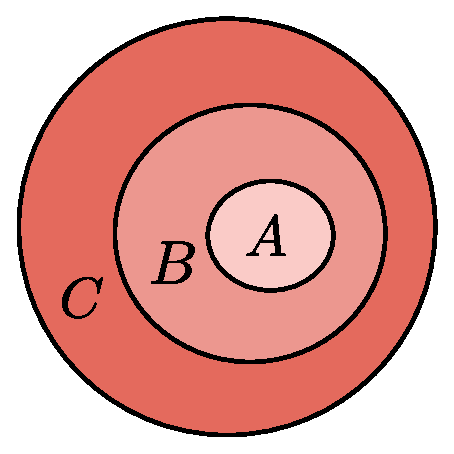
\includegraphics[width=\unitlength]{1.5(a).eps}}%
  \end{picture}%
\endgroup%

	
	%Question 1.5(b)
	\item  \begin{tcolorbox}[
	  colback=Cerulean!5!white,
	  colframe=Cerulean!75!black]
	\textbf{$\bm{A \subset B}$ implies that $\bm{A = A \cap B}$}
	\end{tcolorbox}
	
	\centering
	\begingroup%
  \makeatletter%
  \providecommand\color[2][]{%
    \errmessage{(Inkscape) Color is used for the text in Inkscape, but the package 'color.sty' is not loaded}%
    \renewcommand\color[2][]{}%
  }%
  \providecommand\transparent[1]{%
    \errmessage{(Inkscape) Transparency is used (non-zero) for the text in Inkscape, but the package 'transparent.sty' is not loaded}%
    \renewcommand\transparent[1]{}%
  }%
  \providecommand\rotatebox[2]{#2}%
  \newcommand*\fsize{\dimexpr\f@size pt\relax}%
  \newcommand*\lineheight[1]{\fontsize{\fsize}{#1\fsize}\selectfont}%
  \ifx\svgwidth\undefined%
    \setlength{\unitlength}{170bp}%
    \ifx\svgscale\undefined%
      \relax%
    \else%
      \setlength{\unitlength}{\unitlength * \real{\svgscale}}%
    \fi%
  \else%
    \setlength{\unitlength}{\svgwidth}%
  \fi%
  \global\let\svgwidth\undefined%
  \global\let\svgscale\undefined%
  \makeatother%
  \begin{picture}(1,1)%
    \lineheight{1}%
    \setlength\tabcolsep{0pt}%
    \put(0,0){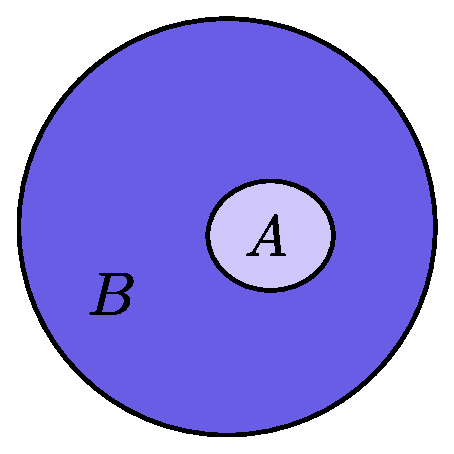
\includegraphics[width=\unitlength]{1.5(b).eps}}%
  \end{picture}%
\endgroup%

	
	%Question 1.5(c)
	\item  \begin{tcolorbox}[
	  colback=Cerulean!5!white,
	  colframe=Cerulean!75!black]
	\textbf{$\bm{A \subset B}$ implies that $\bm{\overline{B} \subset \overline{A}}$}
	\end{tcolorbox}
	
	\centering
	\begingroup%
  \makeatletter%
  \providecommand\color[2][]{%
    \errmessage{(Inkscape) Color is used for the text in Inkscape, but the package 'color.sty' is not loaded}%
    \renewcommand\color[2][]{}%
  }%
  \providecommand\transparent[1]{%
    \errmessage{(Inkscape) Transparency is used (non-zero) for the text in Inkscape, but the package 'transparent.sty' is not loaded}%
    \renewcommand\transparent[1]{}%
  }%
  \providecommand\rotatebox[2]{#2}%
  \newcommand*\fsize{\dimexpr\f@size pt\relax}%
  \newcommand*\lineheight[1]{\fontsize{\fsize}{#1\fsize}\selectfont}%
  \ifx\svgwidth\undefined%
    \setlength{\unitlength}{360bp}%
    \ifx\svgscale\undefined%
      \relax%
    \else%
      \setlength{\unitlength}{\unitlength * \real{\svgscale}}%
    \fi%
  \else%
    \setlength{\unitlength}{\svgwidth}%
  \fi%
  \global\let\svgwidth\undefined%
  \global\let\svgscale\undefined%
  \makeatother%
  \begin{picture}(1,0.6)%
    \lineheight{1}%
    \setlength\tabcolsep{0pt}%
    \put(0,0){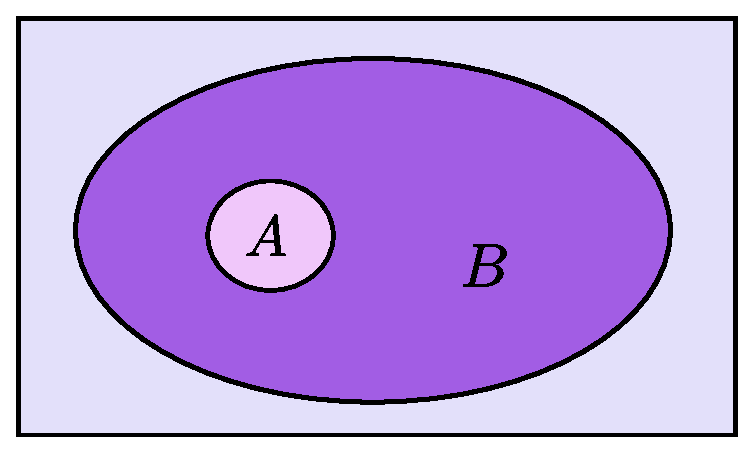
\includegraphics[width=\unitlength]{1.5(c).eps}}%
  \end{picture}%
\endgroup%
	
	%Question 1.5(d)
	\item  \begin{tcolorbox}[
	  colback=Cerulean!5!white,
	  colframe=Cerulean!75!black]
	\textbf{$\bm{A \subset B}$ implies that $\bm{A \cup C \subset B \cup C}$}
	\end{tcolorbox}
	
	\centering
	\begingroup%
  \makeatletter%
  \providecommand\color[2][]{%
    \errmessage{(Inkscape) Color is used for the text in Inkscape, but the package 'color.sty' is not loaded}%
    \renewcommand\color[2][]{}%
  }%
  \providecommand\transparent[1]{%
    \errmessage{(Inkscape) Transparency is used (non-zero) for the text in Inkscape, but the package 'transparent.sty' is not loaded}%
    \renewcommand\transparent[1]{}%
  }%
  \providecommand\rotatebox[2]{#2}%
  \newcommand*\fsize{\dimexpr\f@size pt\relax}%
  \newcommand*\lineheight[1]{\fontsize{\fsize}{#1\fsize}\selectfont}%
  \ifx\svgwidth\undefined%
    \setlength{\unitlength}{360bp}%
    \ifx\svgscale\undefined%
      \relax%
    \else%
      \setlength{\unitlength}{\unitlength * \real{\svgscale}}%
    \fi%
  \else%
    \setlength{\unitlength}{\svgwidth}%
  \fi%
  \global\let\svgwidth\undefined%
  \global\let\svgscale\undefined%
  \makeatother%
  \begin{picture}(1,0.6)%
    \lineheight{1}%
    \setlength\tabcolsep{0pt}%
    \put(0,0){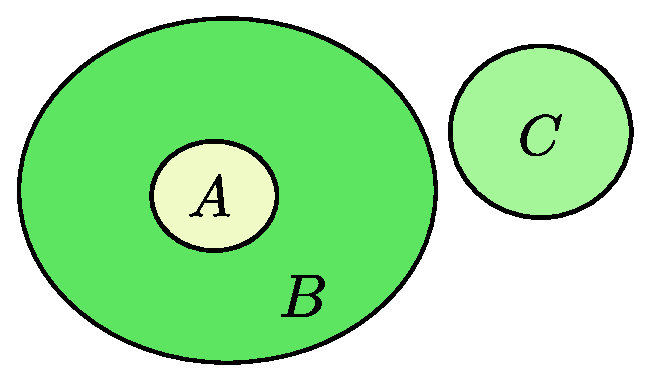
\includegraphics[width=\unitlength]{1.5(d).eps}}%
  \end{picture}%
\endgroup%
	
	%Question 1.5(e)
	\item  \begin{tcolorbox}[
	  colback=Cerulean!5!white,
	  colframe=Cerulean!75!black]
	\textbf{$\bm{A \cap B = \O}$ and $\bm{C \subset A}$ imply that $\bm{B \cap C = \O}$}
	\end{tcolorbox}
	
	\begingroup%
  \makeatletter%
  \providecommand\color[2][]{%
    \errmessage{(Inkscape) Color is used for the text in Inkscape, but the package 'color.sty' is not loaded}%
    \renewcommand\color[2][]{}%
  }%
  \providecommand\transparent[1]{%
    \errmessage{(Inkscape) Transparency is used (non-zero) for the text in Inkscape, but the package 'transparent.sty' is not loaded}%
    \renewcommand\transparent[1]{}%
  }%
  \providecommand\rotatebox[2]{#2}%
  \newcommand*\fsize{\dimexpr\f@size pt\relax}%
  \newcommand*\lineheight[1]{\fontsize{\fsize}{#1\fsize}\selectfont}%
  \ifx\svgwidth\undefined%
    \setlength{\unitlength}{360bp}%
    \ifx\svgscale\undefined%
      \relax%
    \else%
      \setlength{\unitlength}{\unitlength * \real{\svgscale}}%
    \fi%
  \else%
    \setlength{\unitlength}{\svgwidth}%
  \fi%
  \global\let\svgwidth\undefined%
  \global\let\svgscale\undefined%
  \makeatother%
  \begin{picture}(1,0.6)%
    \lineheight{1}%
    \setlength\tabcolsep{0pt}%
    \put(0,0){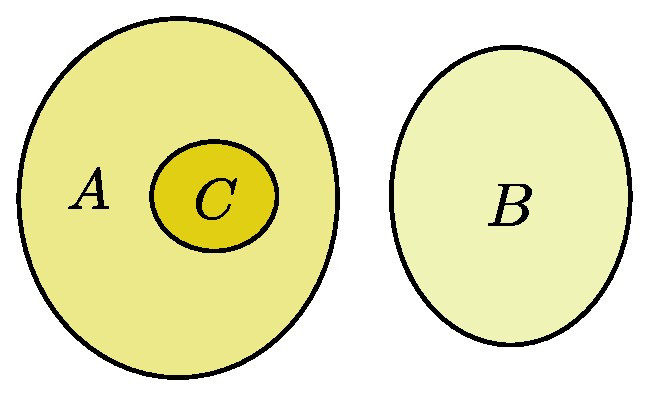
\includegraphics[width=\unitlength]{1.5(e).eps}}%
  \end{picture}%
\endgroup%

	
	\end{enumerate}

%Question 1.6
\item  \begin{tcolorbox}[
  colback=Cerulean!5!white,
  colframe=Cerulean!75!black]
\textbf{Items coming off a production line are marked defective $\bm{(D)}$ or nondefective $\bm{(N)}$. Items are observed and their condition listed. This is continued until two consecutive defectives are produced or four items have been checked, whichever occurs first. Describe a sample space for this experiment.}
\end{tcolorbox}

\boxed{$\{ DD, NDD, NNDD, NNNN, DNNN, NDNN, NNDN, NNND, DNDN, DNND, NDND, DNDD \}$}

%Question 1.7
\item  \begin{tcolorbox}[
  colback=Cerulean!5!white,
  colframe=Cerulean!75!black]
\textbf{[Intentionally blank]}
\end{tcolorbox}

	\begin{enumerate}
	%Question 1.7(a)
	\item  \begin{tcolorbox}[
	  colback=Cerulean!5!white,
	  colframe=Cerulean!75!black]
	\textbf{A box of $\bm{N}$ light bulbs has $\bm{r \ (r < N)}$ bulbs with broken filaments. These bulbs are tested, one by one, until a defective bulb is found. Describe a sample space for this experiment.}
	\end{tcolorbox}
	
	Let $F$ denote the event of testing a non-defective bulb and $T$ for defective. The sample space is
	
	\[ \boxed{ \{ T, FT, FFT, ..., \underbrace{F\cdots F}_{N-r \text{ non-defectives}}T \} } \]
	
	%Question 1.7(b)
	\item  \begin{tcolorbox}[
	  colback=Cerulean!5!white,
	  colframe=Cerulean!75!black]
	\textbf{Suppose that the above bulbs are tested, one by one, until all defectives have been tested. Describe the sample space for this experiment.}
	\end{tcolorbox}
	
	The sample space consists of sequences of every combination of $1, 2, ..., N-r$ non-defectives with the $r$ defectives such that the $r$-th defective is the last of the sequence. For instance, given $i, 1 \leq i \leq N-r$ non-defectives are cycled through to examine all $r$ defectives, there would be $\binom{r-1+i}{i}$ such sequences corresponding to $i$ non-defectives.
	
	\end{enumerate}

%Question 1.8
\item  \begin{tcolorbox}[
  colback=Cerulean!5!white,
  colframe=Cerulean!75!black]
\textbf{Consider four objects, say $\bm{a, b, c,}$ and $\bm{d}$. Suppose that the \textit{order} in which these objects are listed represents the outcome of an experiment. Let the events $\bm{A}$ and $\bm{B}$ be defined as follows: $\bm{A = \{ a \text{ is in the first position}\}}$; $\bm{B = \{b \text{ is in the second position}\}}$.}
\end{tcolorbox}

	\begin{enumerate}
	%Question 1.8(a)
	\item  \begin{tcolorbox}[
	  colback=Cerulean!5!white,
	  colframe=Cerulean!75!black]
	\textbf{List all elements of the sample space.}
	\end{tcolorbox}
	
	\begin{framed}
	\begin{align*}
	B &= \{ abcd, abdc, acbd, acdb, adbc, adcb, bacd, badc, bcad, bcda, bdac, bdca, \\
	&cabd, cadb, cbad, cbda, cdab, cdba, dabc, dacb, dbac, dbca, dcab, dcba \} 
	\end{align*}
	\end{framed}
	
	%Question 1.8(b)
	\item  \begin{tcolorbox}[
	  colback=Cerulean!5!white,
	  colframe=Cerulean!75!black]
	\textbf{List all elements of the events $\bm{A \cap B}$ and $\bm{A \cup B}$.}
	\end{tcolorbox}
	
	\begin{framed}
	\begin{align*}
	A \cap B &= \{ abcd, abdc \} \\
	A \cup B &= \{ abcd, abdc, acbd, acdb, adbc, adcb, cbad, cbda, dbac, dbca \}
	\end{align*}
	\end{framed}
	
	\end{enumerate}

%Question 1.9
\item  \begin{tcolorbox}[
  colback=Cerulean!5!white,
  colframe=Cerulean!75!black]
\textbf{A lot contains items weighing 5, 10, 15, ..., 50 pounds. Assume that at least two items of each weight are found in the lot. Two items are chosen from the lot. Let $\bm{X}$ denote the weight of the first item chosen and $\bm{Y}$ the weight of the second item. Thus the pair of numbers $\bm{(X,Y)}$ represents a single outcome of the experiment. Using the $\bm{XY}$-plane, indicate the sample space and the following events.}
\end{tcolorbox}

The sample space is graphically given by

\begingroup%
  \makeatletter%
  \providecommand\color[2][]{%
    \errmessage{(Inkscape) Color is used for the text in Inkscape, but the package 'color.sty' is not loaded}%
    \renewcommand\color[2][]{}%
  }%
  \providecommand\transparent[1]{%
    \errmessage{(Inkscape) Transparency is used (non-zero) for the text in Inkscape, but the package 'transparent.sty' is not loaded}%
    \renewcommand\transparent[1]{}%
  }%
  \providecommand\rotatebox[2]{#2}%
  \newcommand*\fsize{\dimexpr\f@size pt\relax}%
  \newcommand*\lineheight[1]{\fontsize{\fsize}{#1\fsize}\selectfont}%
  \ifx\svgwidth\undefined%
    \setlength{\unitlength}{216bp}%
    \ifx\svgscale\undefined%
      \relax%
    \else%
      \setlength{\unitlength}{\unitlength * \real{\svgscale}}%
    \fi%
  \else%
    \setlength{\unitlength}{\svgwidth}%
  \fi%
  \global\let\svgwidth\undefined%
  \global\let\svgscale\undefined%
  \makeatother%
  \begin{center}
  \begin{picture}(1,1)%
    \lineheight{1}%
    \setlength\tabcolsep{0pt}%
    \put(0,0){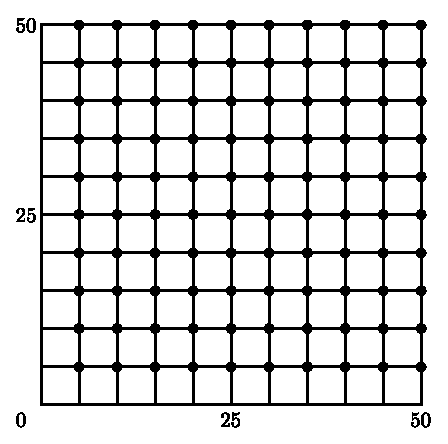
\includegraphics[width=\unitlength]{1.9.eps}}%
  \end{picture}%
  \end{center}
\endgroup%

\par
The described events below are indicated in \textcolor{red}{\textbf{red}}.

	\begin{enumerate}
	%Question 1.9(a)
	\item  \begin{tcolorbox}[
	  colback=Cerulean!5!white,
	  colframe=Cerulean!75!black]
	\textbf{$\bm{\{ X = Y \}}$}
	\end{tcolorbox}
	
	\centering
	\begingroup%
  \makeatletter%
  \providecommand\color[2][]{%
    \errmessage{(Inkscape) Color is used for the text in Inkscape, but the package 'color.sty' is not loaded}%
    \renewcommand\color[2][]{}%
  }%
  \providecommand\transparent[1]{%
    \errmessage{(Inkscape) Transparency is used (non-zero) for the text in Inkscape, but the package 'transparent.sty' is not loaded}%
    \renewcommand\transparent[1]{}%
  }%
  \providecommand\rotatebox[2]{#2}%
  \newcommand*\fsize{\dimexpr\f@size pt\relax}%
  \newcommand*\lineheight[1]{\fontsize{\fsize}{#1\fsize}\selectfont}%
  \ifx\svgwidth\undefined%
    \setlength{\unitlength}{216bp}%
    \ifx\svgscale\undefined%
      \relax%
    \else%
      \setlength{\unitlength}{\unitlength * \real{\svgscale}}%
    \fi%
  \else%
    \setlength{\unitlength}{\svgwidth}%
  \fi%
  \global\let\svgwidth\undefined%
  \global\let\svgscale\undefined%
  \makeatother%
  \begin{picture}(1,1)%
    \lineheight{1}%
    \setlength\tabcolsep{0pt}%
    \put(0,0){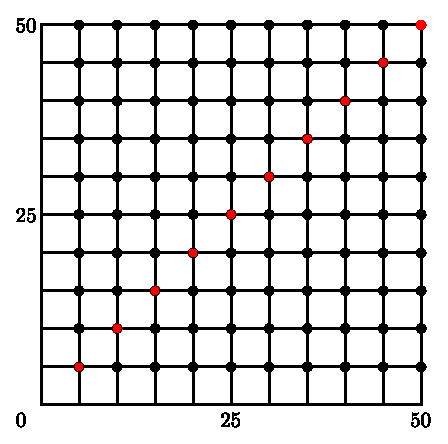
\includegraphics[width=\unitlength]{1.9(a).eps}}%
  \end{picture}%
\endgroup%

	
	%Question 1.9(b)
	\item  \begin{tcolorbox}[
	  colback=Cerulean!5!white,
	  colframe=Cerulean!75!black]
	\textbf{$\bm{\{ Y > X \}}$}
	\end{tcolorbox}
	
	\centering
	\begingroup%
  \makeatletter%
  \providecommand\color[2][]{%
    \errmessage{(Inkscape) Color is used for the text in Inkscape, but the package 'color.sty' is not loaded}%
    \renewcommand\color[2][]{}%
  }%
  \providecommand\transparent[1]{%
    \errmessage{(Inkscape) Transparency is used (non-zero) for the text in Inkscape, but the package 'transparent.sty' is not loaded}%
    \renewcommand\transparent[1]{}%
  }%
  \providecommand\rotatebox[2]{#2}%
  \newcommand*\fsize{\dimexpr\f@size pt\relax}%
  \newcommand*\lineheight[1]{\fontsize{\fsize}{#1\fsize}\selectfont}%
  \ifx\svgwidth\undefined%
    \setlength{\unitlength}{216bp}%
    \ifx\svgscale\undefined%
      \relax%
    \else%
      \setlength{\unitlength}{\unitlength * \real{\svgscale}}%
    \fi%
  \else%
    \setlength{\unitlength}{\svgwidth}%
  \fi%
  \global\let\svgwidth\undefined%
  \global\let\svgscale\undefined%
  \makeatother%
  \begin{picture}(1,1)%
    \lineheight{1}%
    \setlength\tabcolsep{0pt}%
    \put(0,0){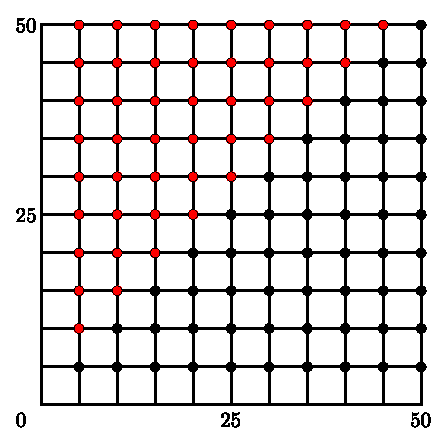
\includegraphics[width=\unitlength]{1.9(b).eps}}%
  \end{picture}%
\endgroup%

	\newpage
	%Question 1.9(c)
	\item  \begin{tcolorbox}[
	  colback=Cerulean!5!white,
	  colframe=Cerulean!75!black]
	\textbf{The second item is twice as heavy as the first item.}
	\end{tcolorbox}
	
	\centering
	\begingroup%
  \makeatletter%
  \providecommand\color[2][]{%
    \errmessage{(Inkscape) Color is used for the text in Inkscape, but the package 'color.sty' is not loaded}%
    \renewcommand\color[2][]{}%
  }%
  \providecommand\transparent[1]{%
    \errmessage{(Inkscape) Transparency is used (non-zero) for the text in Inkscape, but the package 'transparent.sty' is not loaded}%
    \renewcommand\transparent[1]{}%
  }%
  \providecommand\rotatebox[2]{#2}%
  \newcommand*\fsize{\dimexpr\f@size pt\relax}%
  \newcommand*\lineheight[1]{\fontsize{\fsize}{#1\fsize}\selectfont}%
  \ifx\svgwidth\undefined%
    \setlength{\unitlength}{216bp}%
    \ifx\svgscale\undefined%
      \relax%
    \else%
      \setlength{\unitlength}{\unitlength * \real{\svgscale}}%
    \fi%
  \else%
    \setlength{\unitlength}{\svgwidth}%
  \fi%
  \global\let\svgwidth\undefined%
  \global\let\svgscale\undefined%
  \makeatother%
  \begin{picture}(1,1)%
    \lineheight{1}%
    \setlength\tabcolsep{0pt}%
    \put(0,0){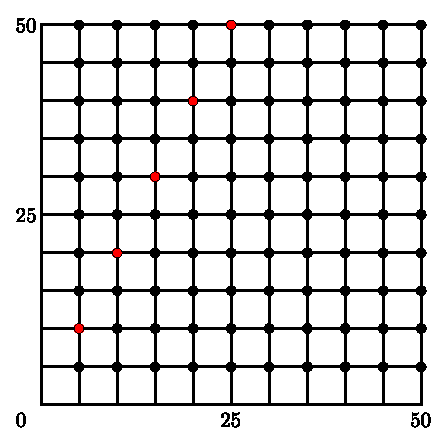
\includegraphics[width=\unitlength]{1.9(c).eps}}%
  \end{picture}%
\endgroup%

	
	%Question 1.9(d)
	\item  \begin{tcolorbox}[
	  colback=Cerulean!5!white,
	  colframe=Cerulean!75!black]
	\textbf{The first item weighs 10 pounds less than the second item.}
	\end{tcolorbox}
	
	\centering
	\begingroup%
  \makeatletter%
  \providecommand\color[2][]{%
    \errmessage{(Inkscape) Color is used for the text in Inkscape, but the package 'color.sty' is not loaded}%
    \renewcommand\color[2][]{}%
  }%
  \providecommand\transparent[1]{%
    \errmessage{(Inkscape) Transparency is used (non-zero) for the text in Inkscape, but the package 'transparent.sty' is not loaded}%
    \renewcommand\transparent[1]{}%
  }%
  \providecommand\rotatebox[2]{#2}%
  \newcommand*\fsize{\dimexpr\f@size pt\relax}%
  \newcommand*\lineheight[1]{\fontsize{\fsize}{#1\fsize}\selectfont}%
  \ifx\svgwidth\undefined%
    \setlength{\unitlength}{216bp}%
    \ifx\svgscale\undefined%
      \relax%
    \else%
      \setlength{\unitlength}{\unitlength * \real{\svgscale}}%
    \fi%
  \else%
    \setlength{\unitlength}{\svgwidth}%
  \fi%
  \global\let\svgwidth\undefined%
  \global\let\svgscale\undefined%
  \makeatother%
  \begin{picture}(1,1)%
    \lineheight{1}%
    \setlength\tabcolsep{0pt}%
    \put(0,0){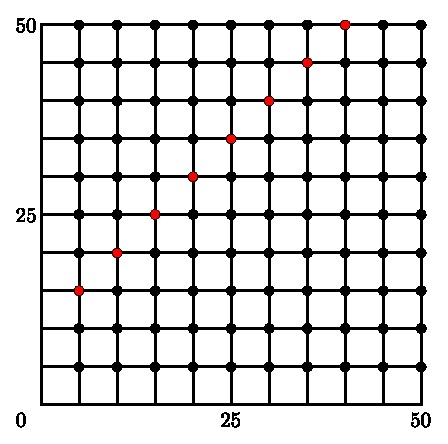
\includegraphics[width=\unitlength]{1.9(d).eps}}%
  \end{picture}%
\endgroup%

	\newpage
	%Question 1.9(e)
	\item  \begin{tcolorbox}[
	  colback=Cerulean!5!white,
	  colframe=Cerulean!75!black]
	\textbf{The average weight of the two items is less than 30 pounds.}
	\end{tcolorbox}
	
	\centering
	\begingroup%
  \makeatletter%
  \providecommand\color[2][]{%
    \errmessage{(Inkscape) Color is used for the text in Inkscape, but the package 'color.sty' is not loaded}%
    \renewcommand\color[2][]{}%
  }%
  \providecommand\transparent[1]{%
    \errmessage{(Inkscape) Transparency is used (non-zero) for the text in Inkscape, but the package 'transparent.sty' is not loaded}%
    \renewcommand\transparent[1]{}%
  }%
  \providecommand\rotatebox[2]{#2}%
  \newcommand*\fsize{\dimexpr\f@size pt\relax}%
  \newcommand*\lineheight[1]{\fontsize{\fsize}{#1\fsize}\selectfont}%
  \ifx\svgwidth\undefined%
    \setlength{\unitlength}{216bp}%
    \ifx\svgscale\undefined%
      \relax%
    \else%
      \setlength{\unitlength}{\unitlength * \real{\svgscale}}%
    \fi%
  \else%
    \setlength{\unitlength}{\svgwidth}%
  \fi%
  \global\let\svgwidth\undefined%
  \global\let\svgscale\undefined%
  \makeatother%
  \begin{picture}(1,1)%
    \lineheight{1}%
    \setlength\tabcolsep{0pt}%
    \put(0,0){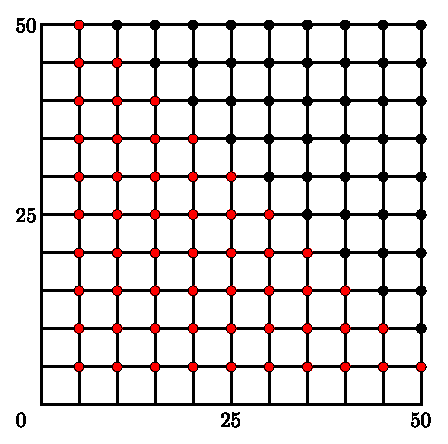
\includegraphics[width=\unitlength]{1.9(e).eps}}%
  \end{picture}%
\endgroup%

	\end{enumerate}

%Question 1.10
\item  \begin{tcolorbox}[
  colback=Cerulean!5!white,
  colframe=Cerulean!75!black]
\textbf{During a 24-hour period, at some time $\bm{X}$, a switch is put into ``ON" position. Subsequently, at some future time $\bm{Y}$ (still during that same 24-hour period) the switch is put into the ``OFF" position. Assume that $\bm{X}$ and $\bm{Y}$ are measured in hours on the time axis with the beginning of the time period as the origin. The outcome of the experiment consists of the pair of numbers $\bm{(X,Y)}$.}
\end{tcolorbox}

The sample space and specific events are described below in the shaded \textcolor{gray}{\textbf{gray}} area.

	\begin{enumerate}
	%Question 1.10(a)
	\item  \begin{tcolorbox}[
	  colback=Cerulean!5!white,
	  colframe=Cerulean!75!black]
	\textbf{Describe the sample space.}
	\end{tcolorbox}
	
	\centering
	\begingroup%
  \makeatletter%
  \providecommand\color[2][]{%
    \errmessage{(Inkscape) Color is used for the text in Inkscape, but the package 'color.sty' is not loaded}%
    \renewcommand\color[2][]{}%
  }%
  \providecommand\transparent[1]{%
    \errmessage{(Inkscape) Transparency is used (non-zero) for the text in Inkscape, but the package 'transparent.sty' is not loaded}%
    \renewcommand\transparent[1]{}%
  }%
  \providecommand\rotatebox[2]{#2}%
  \newcommand*\fsize{\dimexpr\f@size pt\relax}%
  \newcommand*\lineheight[1]{\fontsize{\fsize}{#1\fsize}\selectfont}%
  \ifx\svgwidth\undefined%
    \setlength{\unitlength}{216bp}%
    \ifx\svgscale\undefined%
      \relax%
    \else%
      \setlength{\unitlength}{\unitlength * \real{\svgscale}}%
    \fi%
  \else%
    \setlength{\unitlength}{\svgwidth}%
  \fi%
  \global\let\svgwidth\undefined%
  \global\let\svgscale\undefined%
  \makeatother%
  \begin{picture}(1,1)%
    \lineheight{1}%
    \setlength\tabcolsep{0pt}%
    \put(0,0){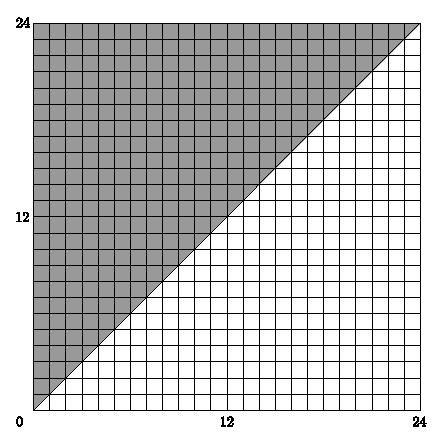
\includegraphics[width=\unitlength]{1.10(a).eps}}%
  \end{picture}%
\endgroup%

	
	%Question 1.10(b)
	\item  \begin{tcolorbox}[
	  colback=Cerulean!5!white,
	  colframe=Cerulean!75!black]
	\textbf{Describe and sketch in the $\bm{XY}$-plane the following events.}
	\end{tcolorbox}
	
		\begin{enumerate}
		%Question 1.10(b)(i)
		\item  \begin{tcolorbox}[
		  colback=Cerulean!5!white,
		  colframe=Cerulean!75!black]
		\textbf{The circuit is on for one hour or less.}
		\end{tcolorbox}
		
		If the circuit is turned on at some time $X$, we must have $X < Y \leq X + 1$.
		
		\begingroup%
  \makeatletter%
  \providecommand\color[2][]{%
    \errmessage{(Inkscape) Color is used for the text in Inkscape, but the package 'color.sty' is not loaded}%
    \renewcommand\color[2][]{}%
  }%
  \providecommand\transparent[1]{%
    \errmessage{(Inkscape) Transparency is used (non-zero) for the text in Inkscape, but the package 'transparent.sty' is not loaded}%
    \renewcommand\transparent[1]{}%
  }%
  \providecommand\rotatebox[2]{#2}%
  \newcommand*\fsize{\dimexpr\f@size pt\relax}%
  \newcommand*\lineheight[1]{\fontsize{\fsize}{#1\fsize}\selectfont}%
  \ifx\svgwidth\undefined%
    \setlength{\unitlength}{216bp}%
    \ifx\svgscale\undefined%
      \relax%
    \else%
      \setlength{\unitlength}{\unitlength * \real{\svgscale}}%
    \fi%
  \else%
    \setlength{\unitlength}{\svgwidth}%
  \fi%
  \global\let\svgwidth\undefined%
  \global\let\svgscale\undefined%
  \makeatother%
  \begin{center}
  \begin{picture}(1,1)%
    \lineheight{1}%
    \setlength\tabcolsep{0pt}%
    \put(0,0){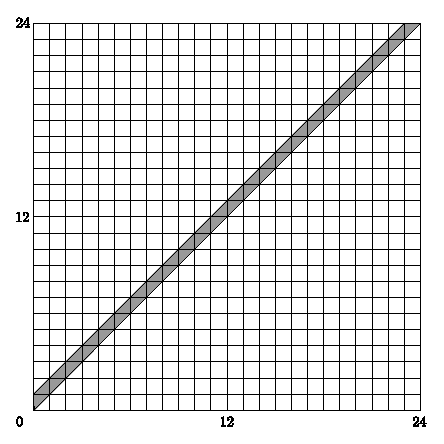
\includegraphics[width=\unitlength]{1.10(b)(i).eps}}%
  \end{picture}%
  \end{center}
\endgroup%

		
		%Question 1.10(b)(ii)
		\item  \begin{tcolorbox}[
		  colback=Cerulean!5!white,
		  colframe=Cerulean!75!black]
		\textbf{The circuit is on at time $\bm{z}$ where $\bm{z}$ is some instant during the given 24-hour period.}
		\end{tcolorbox}
		
		If the circuit is turned on at time $X$, and near-instantaneously turned off at time $Y = X + \Delta X$, we may approximate this as the $45^\circ$ line going through the origin.
		
		\begingroup%
  \makeatletter%
  \providecommand\color[2][]{%
    \errmessage{(Inkscape) Color is used for the text in Inkscape, but the package 'color.sty' is not loaded}%
    \renewcommand\color[2][]{}%
  }%
  \providecommand\transparent[1]{%
    \errmessage{(Inkscape) Transparency is used (non-zero) for the text in Inkscape, but the package 'transparent.sty' is not loaded}%
    \renewcommand\transparent[1]{}%
  }%
  \providecommand\rotatebox[2]{#2}%
  \newcommand*\fsize{\dimexpr\f@size pt\relax}%
  \newcommand*\lineheight[1]{\fontsize{\fsize}{#1\fsize}\selectfont}%
  \ifx\svgwidth\undefined%
    \setlength{\unitlength}{216bp}%
    \ifx\svgscale\undefined%
      \relax%
    \else%
      \setlength{\unitlength}{\unitlength * \real{\svgscale}}%
    \fi%
  \else%
    \setlength{\unitlength}{\svgwidth}%
  \fi%
  \global\let\svgwidth\undefined%
  \global\let\svgscale\undefined%
  \makeatother%
  \begin{center}
  \begin{picture}(1,1)%
    \lineheight{1}%
    \setlength\tabcolsep{0pt}%
    \put(0,0){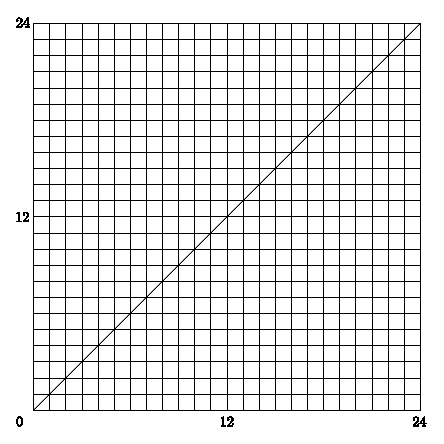
\includegraphics[width=\unitlength]{1.10(b)(ii).eps}}%
  \end{picture}%
  \end{center}
\endgroup%

		\newpage
		%Question 1.10(b)(iii)
		\item  \begin{tcolorbox}[
		  colback=Cerulean!5!white,
		  colframe=Cerulean!75!black]
		\textbf{The circuit is turned on before time $\bm{t_1}$ and turned off after time $\bm{t_2}$ (where again $\bm{t_1 < t_2}$ are two time instants during the specified period).}
		\end{tcolorbox}
		
		Here, we describe the outcomes $0 \leq X < t_1$ and $X \leq Y < t_2$.
		
		\begingroup%
  \makeatletter%
  \providecommand\color[2][]{%
    \errmessage{(Inkscape) Color is used for the text in Inkscape, but the package 'color.sty' is not loaded}%
    \renewcommand\color[2][]{}%
  }%
  \providecommand\transparent[1]{%
    \errmessage{(Inkscape) Transparency is used (non-zero) for the text in Inkscape, but the package 'transparent.sty' is not loaded}%
    \renewcommand\transparent[1]{}%
  }%
  \providecommand\rotatebox[2]{#2}%
  \newcommand*\fsize{\dimexpr\f@size pt\relax}%
  \newcommand*\lineheight[1]{\fontsize{\fsize}{#1\fsize}\selectfont}%
  \ifx\svgwidth\undefined%
    \setlength{\unitlength}{216bp}%
    \ifx\svgscale\undefined%
      \relax%
    \else%
      \setlength{\unitlength}{\unitlength * \real{\svgscale}}%
    \fi%
  \else%
    \setlength{\unitlength}{\svgwidth}%
  \fi%
  \global\let\svgwidth\undefined%
  \global\let\svgscale\undefined%
  \makeatother%
  \begin{center}
  \begin{picture}(1,1)%
    \lineheight{1}%
    \setlength\tabcolsep{0pt}%
    \put(0,0){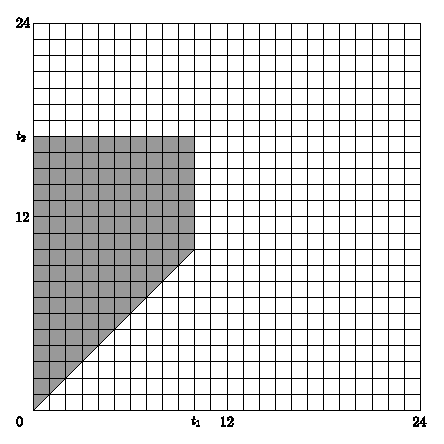
\includegraphics[width=\unitlength]{1.10(b)(iii).eps}}%
  \end{picture}%
  \end{center}
\endgroup%

		
			%Question 1.10(b)(iv)
		\item  \begin{tcolorbox}[
		  colback=Cerulean!5!white,
		  colframe=Cerulean!75!black]
		\textbf{The circuit is on twice as long as it is off.}
		\end{tcolorbox}
		
		The only way to ensure the constraint is met is that the circuit is on for sixteen hours and off for eight. The event is thus described as a straight line between $(0, 16)$ and $(8, 24)$, or all points satisfying the condition $(X, X+16)$.
		
		\begingroup%
  \makeatletter%
  \providecommand\color[2][]{%
    \errmessage{(Inkscape) Color is used for the text in Inkscape, but the package 'color.sty' is not loaded}%
    \renewcommand\color[2][]{}%
  }%
  \providecommand\transparent[1]{%
    \errmessage{(Inkscape) Transparency is used (non-zero) for the text in Inkscape, but the package 'transparent.sty' is not loaded}%
    \renewcommand\transparent[1]{}%
  }%
  \providecommand\rotatebox[2]{#2}%
  \newcommand*\fsize{\dimexpr\f@size pt\relax}%
  \newcommand*\lineheight[1]{\fontsize{\fsize}{#1\fsize}\selectfont}%
  \ifx\svgwidth\undefined%
    \setlength{\unitlength}{216bp}%
    \ifx\svgscale\undefined%
      \relax%
    \else%
      \setlength{\unitlength}{\unitlength * \real{\svgscale}}%
    \fi%
  \else%
    \setlength{\unitlength}{\svgwidth}%
  \fi%
  \global\let\svgwidth\undefined%
  \global\let\svgscale\undefined%
  \makeatother%
  \begin{center}
  \begin{picture}(1,1)%
    \lineheight{1}%
    \setlength\tabcolsep{0pt}%
    \put(0,0){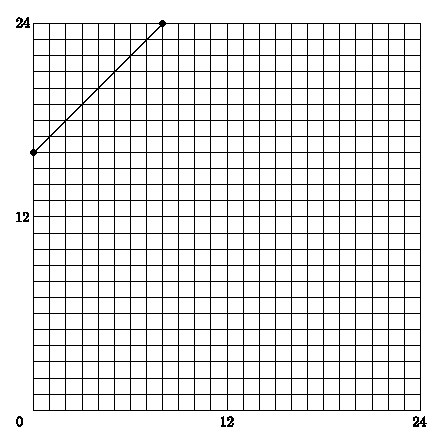
\includegraphics[width=\unitlength]{1.10(b)(iv).eps}}%
  \end{picture}%
  \end{center}
\endgroup%

		
		\end{enumerate}
	\end{enumerate}

%Question 1.11
\item  \begin{tcolorbox}[
  colback=Cerulean!5!white,
  colframe=Cerulean!75!black]
\textbf{Let $\bm{A, B,}$ and $\bm{C}$ be three events associated with an experiment. Express the following verbal statements in set notation.}
\end{tcolorbox}

	\begin{enumerate}
	%Question 1.11(a)
	\item  \begin{tcolorbox}[
	  colback=Cerulean!5!white,
	  colframe=Cerulean!75!black]
	\textbf{At least one of the events occurs.}
	\end{tcolorbox}
	
	\boxed{A \cup B \cup C}
	
	%Question 1.11(b)
	\item  \begin{tcolorbox}[
	  colback=Cerulean!5!white,
	  colframe=Cerulean!75!black]
	\textbf{Exactly one of the events occurs.}
	\end{tcolorbox}
	
	\boxed{[\overline{A} \cap \overline{B} \cap C] \cup [A \cap \overline{B} \cap \overline{C}] \cup [\overline{A} \cap B \cap C]}
	
	%Question 1.11(c)
	\item  \begin{tcolorbox}[
	  colback=Cerulean!5!white,
	  colframe=Cerulean!75!black]
	\textbf{Exactly two of the events occur.}
	\end{tcolorbox}
	
	\boxed{[\overline{A} \cap B \cap C] \cup [A \cap \overline{B} \cap C] \cup [A \cap B \cap \overline{C}]}
	
	%Question 1.11(d)
	\item  \begin{tcolorbox}[
	  colback=Cerulean!5!white,
	  colframe=Cerulean!75!black]
	\textbf{Not more than two of the events occur simultaneously.}
	\end{tcolorbox}
	
	\boxed{\overline{A \cap B \cap C}}
	\end{enumerate}

%Question 1.12
\item  \begin{tcolorbox}[
  colback=Cerulean!5!white,
  colframe=Cerulean!75!black]
\textbf{Prove Theorem 1.4.}
\end{tcolorbox}

\begin{thm}
If $A, B,$ and $C$ are any three events, then

\[ P(A \cup B \cup C) = P(A) + P(B) + P(C) - P(A \cap B) - P(A \cap C) - P(B \cap C) + P(A \cap B \cap C) \]
\end{thm}

\begin{proof}
We know that for any events $X,Y$,

\[ P(X \cup Y) = P(X) + P(Y) - P(X \cap Y) \]

Let $X = A \cup B, Y = C$. Then

\begin{align*}
P(A \cup B \cup C) &= P(A \cup B) + P(c) - P((A \cup B) \cap C) \\
&= P(A) + P(B) + P(C) - P(A \cap B) - P((A \cap C) \cup (B \cap C)) \\
&= P(A) + P(B) + P(C) - P(A \cap B) - P(A \cap C) - P(B \cap C) + P(A \cap B \cap C)
\end{align*}
\end{proof}

%Question 1.13
\item  \begin{tcolorbox}[
  colback=Cerulean!5!white,
  colframe=Cerulean!75!black]
\textbf{[Intentionally blank]}
\end{tcolorbox}

	\begin{enumerate}
	%Question 1.13(a)
	\item  \begin{tcolorbox}[
	  colback=Cerulean!5!white,
	  colframe=Cerulean!75!black]
	\textbf{Show that for any two events, $\bm{A_1}$ and $\bm{A_2}$, we have $\bm{P(A_1 \cup A_2) \leq P(A_1) + P(A_2)}$.}
	\end{tcolorbox}
	
	\begin{proof} We know that $P(A_1 \cup A_2) = P(A_1) + P(A_2) - P(A_1 \cap A_2)$. It immediately follows that $P(A_1 \cup A_2) \leq P(A_1 \cup A_2) + P(A_1 \cap A_2) = P(A_1) + P(A_2)$. 
	\end{proof}
	
	%Question 1.13(b)
	\item  \begin{tcolorbox}[
	  colback=Cerulean!5!white,
	  colframe=Cerulean!75!black]
	\textbf{Show that for any $\bm{n}$ events $\bm{A_1, ..., A_n}$, we have}
	
	\[ \bm{P(A_1 \cup \cdots \cup A_n) \leq P(A_1) + \cdots + P(A_n)} \]
	
	\textbf{[\textit{Hint:} Use mathematical induction. The result stated in (b) is called Boole's inequality.]}
	\end{tcolorbox}
	
	By part (a), $P(A_1 \cup A_2) \leq P(A_1) + P(A_2)$. Now suppose that the result holds for $n$ events. Then by our induction hypothesis,
	
	\[
	P \bigg( \bigg( \bigcup^n_{i=1} A_i \bigg) \cup A_{n+1} \bigg) = P \bigg( \bigcup^n_{i=1} A_i \bigg) + P (A_{n+1}) - P \bigg( \bigg( \bigcup^n_{i=1} A_i \bigg) \cap A_{n+1} \bigg) \leq \sum^{n+1}_{i=1} P(A_i) - P \bigg( \bigg( \bigcup^n_{i=1} A_i \bigg) \cap A_{n+1} \bigg)
	\]
	
	Since $0 \leq P \big( \big( \bigcup^n_{i=1} A_i \big) \cap A_{n+1} \big) \leq 1$, it follows that
	
	\[ P \bigg( \bigg( \bigcup^n_{i=1} A_i \bigg) \cup A_{n+1} \bigg) = \boxed{P \bigg( \bigcup^n_{i=1} A_i \bigg) \leq \sum^{n+1}_{i=1} P(A_i)} \]
	\end{enumerate}

\newpage
%Question 1.14
\item  \begin{tcolorbox}[
  colback=Cerulean!5!white,
  colframe=Cerulean!75!black]
\textbf{Theorem 1.3 deals with the probability that \textit{at least one} of the two events $\bm{A}$ or $\bm{B}$ occurs. The following statement deals with the probability that \textit{exactly one} of the events $\bm{A}$ or $\bm{B}$ occurs. Show that}

\[ \bm{[P(A \cap \overline{B}) \cup (B \cap \overline{A})] = P(A) + P(B) - 2P(A \cap B)} \]
\end{tcolorbox}

\begin{proof}

Meyer Theorem 1.3 states

\begin{thm}
If $A$ and $B$ are \textit{any} two events, then

\[ P(A \cup B) = P(A) + P(B) - P(A \cap B) \]
\end{thm}

The intuition to appeal to here is to observe that $A \cap \overline{B}$ and $B \cap \overline{A}$ are mutually exclusive events. We formally prove this as follows:

\begin{proof}
Let $a \in A \cap \overline{B}$. Then $a \in A, \overline{B}$, so $a \notin B$ and $a \notin B \cap \overline{A}$. Conversely, let $a' \in B \cap \overline{A}$, then $a' \in B, \overline{A}$, so $a' \notin A$, then $a' \notin A \cap \overline{B}$. Thus $(A \cap \overline{B}) \cap (B \cap \overline{A}) = \O$, establishing the mutual exclusivity of these events.
\end{proof}

Using the mutual exclusive property, we know that $P[(A \cap \overline{B}) \cup (B \cap \overline{A})] = P(A \cap \overline{B}) + P(B \cap \overline{A})$. We can also see that

\[ (A \cap \overline{B}) \cup (A \cap B) \quad \text{and} \quad (B \cap \overline{A}) \cup (A \cap B) = B \]

and moreover, that $A \cap \overline{B}, B \cap \overline{A}$, and $A \cap B$ are all disjoint. Thus we have

\begin{align*}
P(A) &= P[(A \cap \overline{B}) \cup (A \cap B)] = P(A \cap \overline{B}) + P(A \cap B) \\
P(B) &= P[(B \cap \overline{A}) \cup (A \cap B)] = P(B \cap \overline{A}) + P(A \cap B)
\end{align*}

Substituting $P(A \cap \overline{B}) = P(A) - P(A \cap B)$ and $P(B \cap \overline{A}) = P(B) - P(A \cap B)$ yields our desired result.

\end{proof}

%Question 1.15
\item  \begin{tcolorbox}[
  colback=Cerulean!5!white,
  colframe=Cerulean!75!black]
\textbf{A certain type of electric motor fails either by seizure of the bearings, or by burning out of the electric windings, or by wearing out of the brushes. Suppose that seizure is twice as likely as burning out, which is four times as likely as brush wearout. What is the probability that failure will be by each of these three mechanisms?}
\end{tcolorbox}

Let $P(\text{brush wearout}) = p$. Then $P(\text{burning out}) = 4p$ and $P(\text{seizure}) = 8p$. Assuming mutual exclusivity of each event, we must have $13p = 1$ or $p = 1/13$. \\
Then $\boxed{P(\text{brush wearout}) = 1/13, P(\text{burning out}) = 4/13, P(\text{seizure}) = 8/13}$.

%Question 1.16
\item  \begin{tcolorbox}[
  colback=Cerulean!5!white,
  colframe=Cerulean!75!black]
\textbf{Suppose that $\bm{A}$ and $\bm{B}$ are events for which $\bm{P(A) = x, P(B) = y,}$ and $\bm{P(A \cap B) = z}$. Express each of the following probabilities in terms of $\bm{x, y,}$ and $\bm{z}$.}
\end{tcolorbox}

	\begin{enumerate}
	%Question 1.16(a)
	\item  \begin{tcolorbox}[
	  colback=Cerulean!5!white,
	  colframe=Cerulean!75!black]
	\textbf{$\bm{P(\overline{A} \cup \overline{B})}$}
	\end{tcolorbox}
	
	\begin{align*}
	P(\overline{A} \cup \overline{B}) &= P(\overline{A}) + P(\overline{B}) - P(\overline{A} \cap \overline{B}) \\
	&= (1 - P(A)) + (1 - P(B)) - (1 - P(A \cup B)) \\
	&= 2 - (P(A) + P(B)) - (1 - (P(A) + P(B) - P(A \cap B))) \\
	&= 2 - (x+y) + x + y - z = \boxed{1 - z}
	\end{align*}
	
	For the following problems, we recall the identities from Problem 1.14:

	\begin{align*}
	P(A) &= P(A \cap \overline{B}) + P(A \cap B) \\
	P(B) &= P(B \cap \overline{A}) + P(A \cap B) 
	\end{align*}
	
	%Question 1.16(b)
	\item  \begin{tcolorbox}[
	  colback=Cerulean!5!white,
	  colframe=Cerulean!75!black]
	\textbf{$\bm{P(\overline{A} \cap B)}$}
	\end{tcolorbox}
	
	\[ P(\overline{A} \cap B) = P(B) - P(A \cap B) = \boxed{y-z} \]
	
	%Question 1.16(c)
	\item  \begin{tcolorbox}[
	  colback=Cerulean!5!white,
	  colframe=Cerulean!75!black]
	\textbf{$\bm{P(\overline{A} \cup B)}$}
	\end{tcolorbox}
	
	\begin{align*}
	P(\overline{A} \cup B) &= P(\overline{A}) + P(B) - P(\overline{A} \cap B) \\
	&= (1 - P(A)) + P(B) - P(\overline{A} \cap B) \\
	&= 1 - x + y - y + z = \boxed{1 - x + z}
	\end{align*}
	
	%Question 1.16(d)
	\item  \begin{tcolorbox}[
	  colback=Cerulean!5!white,
	  colframe=Cerulean!75!black]
	\textbf{$\bm{P(\overline{A} \cap \overline{B})}$}
	\end{tcolorbox}
	
	\[ P(\overline{A} \cap \overline{B}) = 1 - P(A \cup B) = 1 - (P(A) + P(B) - P(A \cap B)) = \boxed{1 - x - y + z} \]
	\end{enumerate}

%Question 1.17
\item  \begin{tcolorbox}[
  colback=Cerulean!5!white,
  colframe=Cerulean!75!black]
\textbf{Suppose that $\bm{A, B,}$ and $\bm{C}$ are events such that $\bm{P(A) = P(B) = P(C) = \frac{1}{4}}$, $\bm{P(A \cap B) = P(C \cap B) = 0}$, and $\bm{P(A \cap C) = \frac{1}{8}}$. Evaluate the probability that at least one of events $\bm{A, B,}$ or $\bm{C}$ occurs.}
\end{tcolorbox}

Since $P(A \cap B) = P(C \cap B) = 0$ implies $A \cap B = C \cap B = \O$, we must also have $A \cap B \cap C = \O$ which implies $P(A \cap B \cap C) = 0$. By Theorem 1.4,

\begin{align*}
P(A \cup B \cup C) &= P(A) + P(B) + P(C) - P(A \cap B) - P(A \cap C) - P(B \cap C) + P(A \cap B \cap C) \\
&= 1/4 + 1/4 + 1/4 - 1/8 \\
&= \boxed{5/8}
\end{align*}

%Question 1.18
\item  \begin{tcolorbox}[
  colback=Cerulean!5!white,
  colframe=Cerulean!75!black]
\textbf{An installation consists of two boilers and one engine. Let the event $\bm{A}$ be ethat the engine is in good condition, while the events $\bm{B_k (k = 1, 2)}$ are the events that the $\bm{k}$th boiler is in good condition. The event $\bm{C}$ is that the installation can operate. If the installation is operative whenever the engine and at least one boiler function, express $\bm{C}$ and $\bm{\overline{C}}$ in terms of $\bm{A}$ and the $\bm{B_i's}$.}
\end{tcolorbox}

$\boxed{C = (A \cap B_1) \cup (A \cap B_2)}$ and $\overline{C} = (\overline{A \cap B_1}) \cap (\overline{A \cap B_2}) = \boxed{(\overline{A} \cup \overline{B_1}) \cap (\overline{A} \cup \overline{B_2})}$

%Question 1.19
\item  \begin{tcolorbox}[
  colback=Cerulean!5!white,
  colframe=Cerulean!75!black]
\textbf{A mechanism has two types of parts, say I and II. Suppose that there are two of type I and three of type II. Define the events $\bm{A_k, k = 1, 2,}$ and $\bm{B_j, j = 1, 2, 3}$ as follows: $\bm{A_k}$: the $\bm{k}$th unit of type I is functioning properly; $\bm{B_j}$: the $\bm{j}$th unit of type II is functioning properly. Finally, let $\bm{C}$ represent the event: the mechanism functions. Given that the mechanism functions if at least one unit of type I and at least two units of type II function, express the event $\bm{C}$ in terms of the $\bm{A_K}$'s and $\bm{B_j}$'s.}
\end{tcolorbox}

$\boxed{C = (A_1 \cup A_2) \cap ((B_1 \cap B_2) \cup (B_1 \cap B_3) \cup (B_2 \cap B_3))}$

\end{enumerate}

\newpage


% ============================================================================
% Chapter 2 - Finite Sample Spaces
% ============================================================================
% Restart the numbered theorem environments so each chapter numbers its own
% corollaries and propositions exactly as it did as a standalone document.
\setcounter{cor}{0}
\setcounter{prop}{0}
\setcounter{cor*}{0}

\phantomsection
\addcontentsline{toc}{section}{Solutions to Chapter 2: Finite Sample Spaces}
\section*{Solutions to Chapter 2: Finite Sample Spaces}

\begin{enumerate}[label=2.\arabic*]
\itemsep0em 
%Question 2.1
\item  \begin{tcolorbox}[
  colback=Cerulean!5!white,
  colframe=Cerulean!75!black]
\textbf{The following group of persons is in a room: 5 men over 21, 4 men under 21, 6 women over 21, and 3 women under 21. One person is chosen at random. The following events are defined: $\bm{A = \{\text{the person is over 21} \}}$; $\bm{B = \{ \text{the person is under 21} \}}$; $\bm{C = \{ \text{the person is male} \}}$; $\bm{D = \text{the person is female}}$. Evaluate the following.}
\end{tcolorbox}

	\begin{enumerate}
	\item \begin{tcolorbox}[
  colback=Cerulean!5!white,
  colframe=Cerulean!75!black]
  $\bm{P(B \cup D)}$
  \end{tcolorbox}
	
	$P(B \cup D) = \boxed{13/18}$
	
	\item \begin{tcolorbox}[
  colback=Cerulean!5!white,
  colframe=Cerulean!75!black]
	$\bm{P(\bar{A} \cap \bar{C})}$
	\end{tcolorbox}
	
	$P(\bar{A} \cap \bar{C}) = \boxed{1/6}$
	
	\end{enumerate}
	
%Question 2.2
\item \begin{tcolorbox}[
  colback=Cerulean!5!white,
  colframe=Cerulean!75!black]
\textbf{Ten persons in a room are wearing badges marked 1 through 10. Three persons are chosen at random, and asked to leave the room simultaneously. Their badge number is noted.}
\end{tcolorbox}

	\begin{enumerate}
	\item  \begin{tcolorbox}[
  colback=Cerulean!5!white,
  colframe=Cerulean!75!black]
	\textbf{What is the probability that the smallest badge number is 5?}
	\end{tcolorbox}
	
	\textbf{Permutation approach.} There are $\Perm{10}{3} = \frac{10!}{7!}$ ways to arrange a trio from a group of ten. Now, there are six badges numbered 5,...,10, inclusive. Thus, there are $\Perm{6}{3} = \frac{6!}{3!}$ ways to arrange a trio involving the six highest numbers. The aim is to now determine how many of those trios actually contain 5. Since 5 is the lowest number in choosing only from this group, if the person with badge 5 is in the trio, then 5 will necessarily be the lowest number. Then the next step is to count the number of trios that do not contain badge 5; namely, the total arrangements of trios from the numbers 6, ..., 10. There are five such numbers, meaning there are $\Perm{5}{3} = \frac{5!}{2!}$ such trios. Less the total arrangements from the trios excluding 5 from the total arrangements of trios from the six highest numbers and divide by the total number of trios from the group of ten to calculate: $(\Perm{6}{3} - \Perm{5}{3}) / \Perm{10}{3} = \boxed{1/12}$.
	
	\textbf{Combination approach.} There are $\binom {10}{3} = \frac{10!}{3!7!}$ ways to choose 3 from a group of 10. Since there are five people with badges greater than 5, if 5 is fixed as the lowest badge number, then there are $\binom 52 = \frac{5!}{2! 3!}$ ways of choosing the remaining two people of those five. Ergo, there is a $\binom{5}{2} / \binom {10}{3} = \boxed{1/12}$ probability that the smallest badge number is 5.
	
	\item \begin{tcolorbox}[
  colback=Cerulean!5!white,
  colframe=Cerulean!75!black]
	\textbf{What is the probability that the largest badge number is 5?}
	\end{tcolorbox}
	
	\textbf{Permutation approach.} As before, there are $\Perm{10}{3} = \frac{10!}{7!}$ ways to arrange a trio from a group of ten. Instead of six badges as previously considered, now there are only five badges in the group numbered 1, ..., 5, inclusive. From this group, there are $\Perm{5}{3} = \frac{5!}{2!}$ arrangements. Now we must less this number of arrangements with the number of arrangements not including badge 5 in the trio, i.e., the trios formed from the group 1,..., 4. This latter arrangement totals simply to $\Perm{4}{3} = \frac{4!}{1!}$. Then the probability is calculated by $(\Perm{5}{3} - \Perm{4}{3}) / \Perm{10}{3} = \boxed{1/20}$. 
	
	\textbf{Combination approach.} Now, there are four people with a badge number less than 5. Thus in fixing 5 as the largest badge number of the trio, there are $\binom 42 = \frac{4!}{2!2!}$ ways of choosing the remaining two people. Proceeding as in part (a), there is a $\binom{4}{2} / \binom {10}{3} = \boxed{1/20}$ probability that the largest badge number is 5.
	
	In both (a) and (b), the combination approach proved simpler. 
	\end{enumerate}
	
%Question 2.3
\item \begin{enumerate}
	\item \begin{tcolorbox}[
  colback=Cerulean!5!white,
  colframe=Cerulean!75!black]
	\textbf{Suppose that the three digits 1, 2, and 3 are written down in random order. What is the probability that at least one digit will occupy its proper place?}
	\end{tcolorbox}
	
	\textbf{Note: The following four problems deal with the inclusion-exclusion principle. Refer to Theorem 1.4 in Meyer.}
	
	There are $3! = 6$ ways to write down the three digits:
	
	\[ \{ (123), (132), (213), (231), (312), (321) \} \]
	
	We can apply Theorem 1.4 of Meyer, where $A$ is one of the digits occupies the correct spot, $B$ for two, and $C$ for all three. Then:
	
	\begin{align*}
	P(A \cup B \cup C) &= P(A) + P(B) + P(C) - P(A \cap B) - P(A \cap C) - P(B \cap C) + P(A \cap B \cap C) \\
	&= 4/6 + 1/6 + 1/6 - 1/6 - 1/6 - 1/6 + 1/6 = \boxed{2/3}
	\end{align*}
	
	We find that the probability of at least one digit occupying its proper place is $\boxed{2/3}$, namely the outcomes $\{ (123), (132), (213), (321)\}$. This approach of defining the events in the aforementioned manner is fine for small $n$, but will become increasingly cumbersome for higher $n$.
	
	A generalized plan of attack on this problem, known as a class of problem called \textbf{derangement}, is to redefine the events as:
	
	\[ A_i = \{ \text{$i$-th digit is in its correct position} \} \]
	
	which is a clearer way to think than attempting to figure out the outcomes corresponding to $k$ digits being located in their correct position, an increasingly difficult task for increasing $n$. Then for $n$ numbers, the 	probability that \textbf{one} of the numbers will be in the correct position will be:
	
	\[ \frac{(n-1)!}{n!} \]
	
	Similarly, the probability that \textbf{two} numbers will occupy their correct position is:
	
	\[ \frac{(n-2)!}{n!} \]
	
	and so on and so forth. For $n = 3$, the application of the inclusion-exclusion principle looks like:
	
	\begin{align*}
	P(A \cup B \cup C) &= P(A) + P(B) + P(C) - P(A \cap B) - P(A \cap C) - P(B \cap C) + P(A \cap B \cap C) \\
	&= \frac{2!}{3!} +  \frac{2!}{3!} +  \frac{2!}{3!} - \frac{1!}{3!} -  \frac{1!}{3!} -  \frac{1!}{3!} +  \frac{1!}{3!} = \boxed{2/3}
	\end{align*}
%Question 2.3(b)
	\item \begin{tcolorbox}[
  colback=Cerulean!5!white,
  colframe=Cerulean!75!black] \textbf{Same as (a) with the digits 1, 2, 3, and 4.}
	\end{tcolorbox}
	
	There are $4! = 24$ total arrangements of the digits 1 through 4. Applying the inclusion-exclusion principle, we want to find:
	
	\[ P\Bigg( \bigcup^4_{k=1} A_k \Bigg) = \sum_{i = 1}^4 P(A_i) - \sum_{i < j = 2}^4 P(A_i \cap A_j) + \sum_{i < j < r = 3}^4 P(A_i \cap A_j \cap A_r) - P \Bigg( \bigcap^4_{k=1} A_k \Bigg) \]
	
	where each $A_k$ corresponds to the event where the $k$-th digit occupies its correct position. It follows that the probabilities for when 1, 2, 3, or 4 of the digits are in their correct position will be $3! / 4!, 2! / 4!, 1! / 4!$, and $0! / 4!$, respectively. The next step is to determine how many terms are in each of the summations. But this is merely the problem of choosing $1 < k < n$ objects out of $n$. Therefore, the solution is given by:
	
	\begin{align*}
	P\Bigg( \bigcup^4_{k=1} A_k \Bigg) &= \sum_{i = 1}^4 P(A_i) - \sum_{i < j = 2}^4 P(A_i \cap A_j) + \sum_{i < j < r = 3}^4 P(A_i \cap A_j \cap A_r) - P \Bigg( \bigcap^4_{k=1} A_k \Bigg)  \\
	&= \binom {4}{1} \frac{3!}{4!} - \binom {4}{2} \frac{2!}{4!} + \binom{4}{3} \frac{1!}{4!} - \binom{4}{4} \frac{0!}{4!} = \boxed{5/8}
	\end{align*}

\newpage
%Question 2.3(c)
	\item  \begin{tcolorbox}[
  colback=Cerulean!5!white,
  colframe=Cerulean!75!black]
  \textbf{Same as (a) with the digits $\bm{1, 2, 3, ..., n}$. }
	\end{tcolorbox}
	
	Proceeding with the analogous logic as in the previous two problems:
	
	\begin{align*}
	P\Bigg( \bigcup^n_{k=1} A_k \Bigg) &= \sum^n_{k=1} (-1)^{k-1} \binom{n}{k} \frac{(n-k)!}{n!} \\
	&= \boxed{ \sum^n_{k=1} (-1)^{k-1} \frac{1}{k!} }
	\end{align*}

%Question 2.3(d)
	\item \begin{tcolorbox}[
  colback=Cerulean!5!white,
  colframe=Cerulean!75!black]
   \textbf{Discuss the answer to (c) if $\bm{n}$ is large.}
	\end{tcolorbox}
	
	Now, recall the fact that
	
	\[ e^{-1} = \sum^\infty_{k = 0} \frac{(-1)^k}{k!} \]
	
	From this we can deduce that the limit of the previous solution as $n \rightarrow \infty$ is $\boxed{1 - e^{-1}}$.
	\end{enumerate}
%Question 2.4
\item \begin{tcolorbox}[
  colback=Cerulean!5!white,
  colframe=Cerulean!75!black]
  \textbf{A shipment of 1500 washers contains 400 defective and 1100 nondefective items. Two-hundred washers are chosen at random (without replacement) and classified.}
  \end{tcolorbox}
  
  	\begin{enumerate}
	%Question 2.4(a)
	\item  \begin{tcolorbox}[
  colback=Cerulean!5!white,
  colframe=Cerulean!75!black]
  	\textbf{What is the probability that exactly 90 defective items are found?}
  	 \end{tcolorbox}
	 
	 \textbf{Note: These two questions deal with hypergeometric probabilities.}
	 
	 $\boxed{\frac{\binom{400}{90} \binom{1100}{110}}{\binom{1500}{200}}}$
	 %Question 2.4(b)
	 \item  \begin{tcolorbox}[
  colback=Cerulean!5!white,
  colframe=Cerulean!75!black]
  	\textbf{What is the probability that at least 2 defective items are found?}
  	 \end{tcolorbox}
	 
	 The probability that less than 2 defective items are found (namely, exactly 1 and 0 defective items are found) is:
	 
	 \[ \frac{ \binom{400}{1} \binom{1100}{199} + \binom{400}{0} \binom{1100}{200}}{\binom{1500}{200}} \]
	 
	 Therefore, the probability that at least 2 defective items are found is:
	 
	  \[ \boxed{ 1 - \Bigg[ \frac{ \binom{400}{1} \binom{1100}{199} + \binom{400}{0} \binom{1100}{200}}{\binom{1500}{200}} \Bigg] } \]

	\end{enumerate}
%Question 2.5
\item \begin{tcolorbox}[
  colback=Cerulean!5!white,
  colframe=Cerulean!75!black]
  \textbf{Ten chips numbered 1 through 10 are mixed in a bowl. Two chips numbered $\bm{(X,Y)}$ are drawn from the bowl, successively and without replacement. What is the probability that $\bm{X + Y = 10}$?}
   \end{tcolorbox}
   
   \textbf{Note: The principle to recall here is that of multiplicative probabilities: when two events $\bm{A, B}$ are independent, the probability of both happening ($\bm{P(A \cap B)}$) is the product of the probabilities of the individual events, namely $\bm{P(A)P(B)}$. Should the events be dependent, say $\bm{B}$ depends on $\bm{A}$, then $\bm{P(A \cap B) = P(A) P(B | A)}$ .}
   
   In the first drawing, there are 10 chips to choose from. In the second, there are only 9. By the multiplication principle, there are 90 possible outcomes. For the first round, drawing any chip suffices so long as that chip is not 5 or 10. We cannot choose 10, because no other chip summed with 10 will yield 10, and we also cannot choose 5, because we do not replace the chips, and there is no other number to which 5 can be summed to give us 10. Therefore, there is a $8/10$ odds that chips 5 or 10 are not drawn. In the second round, only 9 chips remain, for which only one will correspond to the first chip to give 10, or a 1/9 chance of drawing that chip. By the multiplicative property of conditional probabilities of dependent events, $(8/10)(1/9) = \boxed{4/45}$.

%Question 2.6
\item \begin{tcolorbox}[
  colback=Cerulean!5!white,
  colframe=Cerulean!75!black]
  \textbf{A lot consists of 10 good articles, 4 with minor defects, and 2 with major defects. One article is chosen at random. Find the probability that:}
  \end{tcolorbox}
  
  	\begin{enumerate}
	%Question 2.6(a)
	\item \begin{tcolorbox}[
  colback=Cerulean!5!white,
  colframe=Cerulean!75!black]
  \textbf{it has no defects,}
  \end{tcolorbox}
  
  Choose one of ten good items out of sixteen total items, $\frac{\binom{10}{1} }{\binom{16}{1}} = \boxed{5/8}$.
  
  	%Question 2.6(b)
  	\item \begin{tcolorbox}[
  colback=Cerulean!5!white,
  colframe=Cerulean!75!black]
  \textbf{it has no major defects,}
  \end{tcolorbox}
  
  Choose one of ten good items or one of 4 minor defect items out of sixteen total items, $\frac{\binom{10}{1} + \binom{4}{1} }{\binom{16}{1}}  = \boxed{7/8}$.
  
    	%Question 2.6(c)
  	\item \begin{tcolorbox}[
  colback=Cerulean!5!white,
  colframe=Cerulean!75!black]
  \textbf{it is either good or has major defects.}
  \end{tcolorbox}
  
  Choose one of ten good items or one of two major defect items,
  \[ P(\text{good} \cup \text{major defects}) = P(\text{good}) + P(\text{major defects}) - P(\text{good} \cap \text{major defects}) = \frac{\binom{10}{1} + \binom{2}{1} }{\binom{16}{1}} - 0 = \boxed{3/4} \]
  In the alternative, take unity less the probability of the complement event, which is choose only items with minor defects, or $1 - 4/16 = \boxed{3/4}$. 

	\end{enumerate}

%Question 2.7
\item \begin{tcolorbox}[
  colback=Cerulean!5!white,
  colframe=Cerulean!75!black]
  \textbf{If from the lot of articles described in Problem 2.6 two articles are chosen (without replacement), find the probability that:}
  \end{tcolorbox}
  	
  	\begin{enumerate}
	%Question 2.7(a)
	\item \begin{tcolorbox}[
  colback=Cerulean!5!white,
  colframe=Cerulean!75!black]
  \textbf{both are good,}
  \end{tcolorbox}
  
  Choose one of ten good articles out of sixteen total articles in the first round, followed by one of nine good articles out of the remaining fifteen articles in the second, invoke dependence of probabilities, $\frac{10}{16} \cdot \frac{9}{15} = \boxed{3/8}$.
  
  All sub-parts below proceed using similar logic of the product of probabilities.
  	
	%Question 2.7(b)
  	\item \begin{tcolorbox}[
  colback=Cerulean!5!white,
  colframe=Cerulean!75!black]
  \textbf{both have major defects,}
  \end{tcolorbox}
  
  	$\frac{2}{16} \cdot \frac{1}{15} = \boxed{1/120}$
 	%Question 2.7(c)
  	\item \begin{tcolorbox}[
  colback=Cerulean!5!white,
  colframe=Cerulean!75!black]
  \textbf{at least one is good,}
  \end{tcolorbox}
  
  	Equivalently, unity less the probability that both are defective.
	
	\[ 1 - \frac{6}{16} \cdot \frac{5}{15} = 1 - \frac{30}{240} = \boxed{7/8} \]
  	%Question 2.7(d)
  	\item \begin{tcolorbox}[
  colback=Cerulean!5!white,
  colframe=Cerulean!75!black]
  \textbf{at most one is good,}
  \end{tcolorbox}
  
  	Equivalently, unity less the probability that both are good. 
	
	\[ 1 - \frac{10}{16} \cdot \frac{9}{15} = 1 - 3/8 = \boxed{ \frac{5}{8} } \]
  	%Question 2.7(e)
  	\item \begin{tcolorbox}[
  colback=Cerulean!5!white,
  colframe=Cerulean!75!black]
  \textbf{exactly one is good,}
  \end{tcolorbox}
  
  \[ \frac{\binom{10}{1} \binom{6}{1} }{\binom{16}{2}} = \boxed{1/2} \]
  	%Question 2.7(f)
  	\item \begin{tcolorbox}[
  colback=Cerulean!5!white,
  colframe=Cerulean!75!black]
  \textbf{neither has major defects,}
  \end{tcolorbox}
  
  \[ \frac{14}{16} \cdot \frac{13}{15} = \boxed{91/120} \]
  	%Question 2.7(g)
  	\item \begin{tcolorbox}[
  colback=Cerulean!5!white,
  colframe=Cerulean!75!black]
  \textbf{neither is good.}
  \end{tcolorbox}
  
  \[ \frac{6}{16} \cdot \frac{5}{15} = \boxed{1/8} \]
	\end{enumerate}
%Question 2.8
\item \begin{tcolorbox}[
  colback=Cerulean!5!white,
  colframe=Cerulean!75!black]
  \textbf{A product is assembled in three stages. At the first stage there are 5 assembly lines, at the second stage there are 4 assembly lines, and at the third stage there are 6 assembly lines. In how many different ways may the product be routed through the assembly process?}
  \end{tcolorbox}
  
  By the multiplicative principle, $5 \cdot 4 \cdot 6 = \boxed{120}$ ways.
%Question 2.9
\item \begin{tcolorbox}[
  colback=Cerulean!5!white,
  colframe=Cerulean!75!black]
  \textbf{An inspector visits 6 different machines during the day. In order to prevent operators from knowing when he will inspect he varies the order of his visits. In how many ways may this be done?}
  \end{tcolorbox}
  
  $\boxed{6!}$ ways.
%Question 2.10
\item \begin{tcolorbox}[
  colback=Cerulean!5!white,
  colframe=Cerulean!75!black]
  \textbf{A complex mechanism may fail at 15 stages. If it fails at 3 stages, in how many ways may this happen?}
  \end{tcolorbox}
  
  $\binom{15}{3} = \boxed{455}$ ways.

%Question 2.11  
\item \begin{tcolorbox}[
  colback=Cerulean!5!white,
  colframe=Cerulean!75!black]
  \textbf{There are 12 ways in which a manufactured item can be a minor defective and 10 ways in which it can be a major defective. In how many ways can 1 minor and 1 major defective occur? 2 minor and 2 major defectives?}
  \end{tcolorbox}
  
  \textbf{1 minor and 1 major defective:} $12 \cdot 10 = \boxed{120}$ ways.
  
  \textbf{2 minor and 2 major defectives:} $\binom{12}{2} \cdot \binom{10}{2} = 66 \cdot 45 = \boxed{2970}$ ways.

%Question 2.12
\item \begin{tcolorbox}[
  colback=Cerulean!5!white,
  colframe=Cerulean!75!black]
  \textbf{A mechanism may be set at any one of four positions, say $\bm{a,b,c,}$ and $\bm{d}$. There are 8 such mechanisms which are inserted into a system.}
  \end{tcolorbox}
  
  	\begin{enumerate}
	%Question 2.12(a)
	\item \begin{tcolorbox}[
  colback=Cerulean!5!white,
  colframe=Cerulean!75!black]
  \textbf{In how many ways may this system be set?}
  \end{tcolorbox}
  
  	Eight mechanisms which each can have one of four positions, so $\boxed{4^8}$ ways.
  	%Question 2.12(b)
  	\item \begin{tcolorbox}[
  colback=Cerulean!5!white,
  colframe=Cerulean!75!black]
  \textbf{Assume that these mechanisms are installed in some preassigned (linear) order. How many ways of setting the system are available if no two adjacent mechanisms are in the same position?}
  \end{tcolorbox}
  
  	The first of the mechanisms can take on any of the four positions. The adjacent mechanism, under the constraint, can only be placed into one of three positions. And so on and so forth for the remaining mechanisms. Therefore, $\boxed{4 \cdot 3^7}$ ways.
  	%Question 2.12(c)
  	\item \begin{tcolorbox}[
  colback=Cerulean!5!white,
  colframe=Cerulean!75!black]
  \textbf{How many ways are available if only positions $\bm{a}$ and $\bm{b}$ are used, and these are used equally often?}
  \end{tcolorbox}
  
  	A simpler way to think about this problem is to ask: for each of the eight mechanisms, how many ways can we choose four of them to place in position $a$? But this is merely $\binom{8}{4} = \boxed{70}$ ways.
	%Question 2.12(d)
  	\item \begin{tcolorbox}[
  colback=Cerulean!5!white,
  colframe=Cerulean!75!black]
  \textbf{How many ways are available if only two different positions are used and one of these positions appears three times as often as the other?}
  \end{tcolorbox}
  
  	For any one pair, there are $\binom{8}{6} = 28$ ways to arrange the mechanisms under the given constraint. There are $\binom{4}{2} = 6$ different pairings. For each of those pairings, one of the positions will appear three times as often as the other, so the number of ways must be doubled to account for the other of the positions appearing three times as often as the initial. Therefore, there are $28 \cdot 6 \cdot 2 = \boxed{336}$ ways.
	
	\end{enumerate}
%Question 2.13
\item \begin{tcolorbox}[
  colback=Cerulean!5!white,
  colframe=Cerulean!75!black]
  \textbf{Suppose that from $\bm{N}$ objects we choose $\bm{n}$ at random, with replacement. What is the probability that no object is chosen more than once? (Suppose that $\bm{n < N}$.)}
  \end{tcolorbox}
  
  There are $N^n$ total ways to choose $n$ objects from a group of $N$, with replacement. There are $\frac{N!}{(N-n)!}$ ways to choose $n$ objects from a group of $N$ under the aforementioned constraint, ergo probability $\boxed{ \frac{N!}{(N-n)! N^n }} $.
%Question 2.14 
\item \begin{tcolorbox}[
  colback=Cerulean!5!white,
  colframe=Cerulean!75!black]
  \textbf{From the letters a, b, c, d, e, and f how many 4-letter code words may be formed if,}
  \end{tcolorbox}
  
  	\begin{enumerate}
	%Question 2.14(a)
	\item \begin{tcolorbox}[
  colback=Cerulean!5!white,
  colframe=Cerulean!75!black]
  \textbf{no letter may be repeated?}
  \end{tcolorbox}
  
  Order matters, so this is a permutation problem. There are $\Perm{6}{4} = \boxed{360}$ words.
  	%Question 2.14(b)
  	\item \begin{tcolorbox}[
  colback=Cerulean!5!white,
  colframe=Cerulean!75!black]
  \textbf{any letter may be repeated any number of times?}
  \end{tcolorbox}
  
  $\boxed{6^4}$ words.
	\end{enumerate}
%Question 2.15
\item \begin{tcolorbox}[
  colback=Cerulean!5!white,
  colframe=Cerulean!75!black]
  \textbf{Suppose that $\binom{99}{5} = a$ and $ \binom{99}{4} = b$. Express $\binom{100}{95} $ in terms of $\bm{a}$ and $\bm{b}$.}
  \end{tcolorbox}
  
  Observe that $\binom{99}{5} = \binom{99}{94} = a$ and $\binom{99}{4} = \binom{99}{95} = b$. Then $\binom{100}{95} = \binom{99}{94} + \binom{99}{95} = \boxed{a + b}$.
%Question 2.16
\item \begin{tcolorbox}[
  colback=Cerulean!5!white,
  colframe=Cerulean!75!black]
  \textbf{A box contains tags marked $\bm{1, 2, ..., n}$. Two tags are chosen at random. Find the probability that the numbers on the tags will be consecutive integers if}
  \end{tcolorbox}
  
  	\begin{enumerate}
	%Question 2.16(a)
	\item \begin{tcolorbox}[
  colback=Cerulean!5!white,
  colframe=Cerulean!75!black]
  \textbf{the tags are chosen without replacement,}
  \end{tcolorbox}
  
  	Equivalently, we find the probability of choosing two consecutive tags when the choice of the first tag is any one of $2, ..., n-1$ or when it is either $1$ or $n$. Call the first case $C_1$ and the second $C_2$. There is a $\frac{n-2}{n}$ probability of the former case in the first draw, and a $\frac{2}{n-1}$ probability of choosing a consecutive tag in the second draw, from which we can deduce $( \frac{n-2}{n} ) ( \frac{2}{n-1} )$ probability of drawing consecutive tags in the first case. For the latter case, there is a $\frac{2}{n}$ probability of drawing $1$ or $n$, and a $\frac{1}{n-1}$ probability of drawing its adjacent tag in the second round. Therefore the probability of drawing consecutive tags in the second case is $( \frac{2}{n} ) ( \frac{1}{n-1} )$. By mutual exclusivity of the two cases (we cannot draw $2, ..., n-1$ and $1$ or $n$ in the first round),
	
	\begin{align*}
	P(C_1 \cup C_2) &= P(C_1) + P(C_2) \\
	&= \Bigg( \frac{n-2}{n} \Bigg) \Bigg( \frac{2}{n-1} \Bigg) + \Bigg( \frac{2}{n} \Bigg) \Bigg( \frac{1}{n-1} \Bigg) = \boxed{ \frac{2}{n} }
	\end{align*}
  	%Question 2.16(b)
  	\item \begin{tcolorbox}[
  colback=Cerulean!5!white,
  colframe=Cerulean!75!black]
  \textbf{the tags are chosen with replacement.}
  \end{tcolorbox}
  
  	Analogous argument as in the case without replacement, but with $n$ in lieu of $n-1$ in the denominator for the second round.
	
	\begin{align*}
	P(C_1 \cup C_2) &= P(C_1) + P(C_2) \\
	&= \Bigg( \frac{n-2}{n} \Bigg) \Bigg( \frac{2}{n} \Bigg) + \Bigg( \frac{2}{n} \Bigg) \Bigg( \frac{1}{n} \Bigg) = \boxed{ \frac{2(n-1)}{n^2} }
	\end{align*}
	\end{enumerate}
%Question 2.17
\item \begin{tcolorbox}[
  colback=Cerulean!5!white,
  colframe=Cerulean!75!black]
  \textbf{How many subsets can be formed, containing at least one member, from a set of 100 elements?}
  \end{tcolorbox}
  
  Equivalently, find the number of ways to choose $k$ from 100 objects, $1 \leq k \leq 100$, and sum each of those ways for all $k$, or \boxed{ \sum_{k = 1}^{100} \binom{100}{k} }.
%Question 2.18
\item \begin{tcolorbox}[
  colback=Cerulean!5!white,
  colframe=Cerulean!75!black]
  \textbf{One integer is chosen at random from the numbers 1, 2, ..., 50. What is the probability that the chosen number is divisible by 6 or by 8?}
  \end{tcolorbox}
  
  The numbers divisible by 6 are $\{ 6, 12, 18, 24, 30, 36, 42, 48 \}$, and by 8 are $\{ 8, 16, 24, 32, 40, 48 \}$. The only numbers divisible by both are $24$ and $48$. Therefore, $P(\text{divisible by 6 or divisible by 8}) = P(\text{divisible by 6}) + P(\text{divisible by 8}) - P(\text{divisible by 6 and 8}) = 8/50 + 6/50 - 2/50 = \boxed{6/25}$.
%Question 2.19
\item \begin{tcolorbox}[
  colback=Cerulean!5!white,
  colframe=Cerulean!75!black]
  \textbf{From 6 positive and 8 negative numbers, 4 numbers are chosen at random (without replacement) and multiplied. What is the probability that the product is a positive number?}
  \end{tcolorbox}
  
  There are $\binom{14}{4}$ total ways to choose 4 numbers out of 14. There are several ways to get a product that is a positive number: by choosing 4 positives, 4 negatives, or 2 positives and 2 negatives. Applying hypergeometric probability and summing the combinations yields:
  
  \begin{align*}
  \frac{\binom{6}{4} + \binom{8}{4} + \binom{6}{2} \cdot \binom{8}{2} }{\binom{14}{4}} &= \frac{ \frac{6!}{2! 4!} + \frac{8!}{4! 4!} + \frac{6!}{2! 4!} \cdot \frac{8!}{2! 6!} }{\frac{14!}{4! 10!}} \\
  &= \frac{15 + 70 + 15\cdot 28}{1001} = \boxed{505/1001}
  \end{align*}
%Question 2.20
\item \begin{tcolorbox}[
  colback=Cerulean!5!white,
  colframe=Cerulean!75!black]
  \textbf{A certain chemical substance is made by mixing 5 separate liquids. It is proposed to pour one liquid into a tank, and then to add the other liquids in turn. All possible combinations must be tested to see which gives the best yield. How many tests must be performed?}
  \end{tcolorbox}
  
  $5! = \boxed{120}$ ways.
  
%Question 2.21
\item \begin{tcolorbox}[
  colback=Cerulean!5!white,
  colframe=Cerulean!75!black]
  \textbf{A lot contains $\bm{n}$ articles. If it is known that $\bm{r}$ of the articles are defective and the articles are inspected in a random order, what is the probability that the $\bm{k}$-th article $\bm{(k \geq r)}$ inspected will be the last defective one in the lot?}
  \end{tcolorbox}
  
  To motivate this problem, first imagine every possible combination of the $n$ articles arranged in a line. Recognize that there are $\binom{n}{r}$ total positions that the $r$ articles can take in the line of $n$ articles; this is equivalent to choosing $r$ objects from $n$. The trickier insight is to ascertain how many arrangements of the $r$ defective articles there are if the last of the $r$ articles is in the $k$-th position. To do so, fix the $r$-th article in the $k$-th position. Then there are $r-1$ remaining objects to arrange in the $k-1$ remaining positions. Simply, there are $\binom{k-1}{r-1}$ ways to do this. Therefore, the probability that the $k$-th article $(k \geq r)$ inspected will be the last defective one in the lot is $\boxed{\binom{k-1}{r-1} / \binom{n}{r}}$.
\end{enumerate}

\newpage


% ============================================================================
% Chapter 3 - Conditional Probability and Independence
% ============================================================================
% Restart the numbered theorem environments so each chapter numbers its own
% corollaries and propositions exactly as it did as a standalone document.
\setcounter{cor}{0}
\setcounter{prop}{0}
\setcounter{cor*}{0}

\phantomsection
\addcontentsline{toc}{section}{Solutions to Chapter 3: Conditional Probability and Independence}
\section*{Solutions to Chapter 3: Conditional Probability and Independence}

Unfinished problems: 3.32

\begin{enumerate}[label=3.\arabic*]
\itemsep0em 
%Question 3.1
\item  \begin{tcolorbox}[
  colback=Cerulean!5!white,
  colframe=Cerulean!75!black]
\textbf{Urn 1 contains $\bm{x}$ white and $\bm{y}$ red balls. Urn 2 contains $\bm{z}$ white and $\bm{v}$ red balls. A ball is chosen at random from urn 1 and put into urn 2. Then a ball is chosen at random from urn 2. What is the probability that this ball is white?}
\end{tcolorbox}

Define the following probabilities: $P(U_1, W)$ for selecting white from urn 1, $P(U_1, R)$ for selecting red from urn 1, $P(U_2, W, W)$ for selecting white from urn 2 given that a white ball has been added, $P(U_2, W, R)$ for selecting white from urn 2 given that a red ball has been added, and $P(U_2, W)$ for selecting white from urn 2 (the desired probability). By the Law of Total Probability, 

\[ P(U_2, W) = P(U_1, W) P(U_2, W, W) + P(U_1, R) P(U_2, W, R) \]

The respective probabilities are $P(U_1, W) = \frac{x}{x+y},  P(U_2, W, W) = \frac{z+1}{z+v+1}, P(U_1, R) = \frac{y}{x+y}, P(U_2, W, R) = \frac{z}{z+v+1}$. Therefore,

\begin{align*}
P(U_2, W) &= \Bigg(  \frac{x}{x+y} \Bigg)  \Bigg( \frac{z+1}{z+v+1} \Bigg) + \Bigg( \frac{y}{x+y} \Bigg) \Bigg( \frac{z}{z+v+1} \Bigg) \\
&= \boxed{ \frac{x(z+1) + yz}{(x+y) (z+v+1)} }
\end{align*}

%Question 3.2
\item  \begin{tcolorbox}[
  colback=Cerulean!5!white,
  colframe=Cerulean!75!black]
\textbf{Two defective tubes get mixed up with two good ones. The tubes are tested, one by one, until both defectives are found.}
\end{tcolorbox}

Here, we need only apply the result of problem 2.21, namely that for $r$ defects in a queue of $n$ items, the probability of finding the last defective item in the $k$-th position is $\binom{k-1}{r-1} / \binom{n}{r}$.

	\begin{enumerate}
	%Question 3.2(a)
	\item  \begin{tcolorbox}[
	  colback=Cerulean!5!white,
	  colframe=Cerulean!75!black]
	\textbf{What is the probability that the last defective tube is obtained on the second test?}
	\end{tcolorbox}
	
	$\binom{1}{1} / \binom{4}{2} = \boxed{1/6}$
	
	%Question 3.2(b)
	\item  \begin{tcolorbox}[
	  colback=Cerulean!5!white,
	  colframe=Cerulean!75!black]
	\textbf{What is the probability that the last defective tube is obtained on the third test?}
	\end{tcolorbox}
	
	$\binom{2}{1} / \binom{4}{2} = \boxed{1/3}$
	
	%Question 3.2(c)
	\item  \begin{tcolorbox}[
	  colback=Cerulean!5!white,
	  colframe=Cerulean!75!black]
	\textbf{What is the probability that the last defective tube is obtained on the fourth test?}
	\end{tcolorbox}
	
	$\binom{3}{1} / \binom{4}{2} = \boxed{1/2}$
	
	%Question 3.2(c)
	\item  \begin{tcolorbox}[
	  colback=Cerulean!5!white,
	  colframe=Cerulean!75!black]
	\textbf{Add the numbers obtained for (a), (b), and (c) above. Is the result surprising?}
	\end{tcolorbox}
	
	$\boxed{1}$. No, by intuitively appealing to each of the outcomes as one partition collectively spanning the whole sample space.

	\end{enumerate}

%Question 3.3
\item  \begin{tcolorbox}[
  colback=Cerulean!5!white,
  colframe=Cerulean!75!black]
\textbf{A box contains 4 bad and 6 good tubes. Two are drawn out together. One of them is tested and found to be good. What is the probability that the other one is also good?}
\end{tcolorbox}

$P(\text{second tube is good} | \text{first tube is good}) = \boxed{5/9}$

%Question 3.4
\item  \begin{tcolorbox}[
  colback=Cerulean!5!white,
  colframe=Cerulean!75!black]
\textbf{In the above problem the tubes are checked by drawing a tube at random, testing it and repeating the process until all 4 bad tubes are located. What is the probability that the fourth bad tube will be located}
\end{tcolorbox}

Here, we need only apply the result of problem 2.21, namely that for $r$ defects in a queue of $n$ items, the probability of finding the last defective item in the $k$-th position is $\binom{k-1}{r-1} / \binom{n}{r}$.

	\begin{enumerate}
	%Question 3.4(a)
	\item  \begin{tcolorbox}[
	  colback=Cerulean!5!white,
	  colframe=Cerulean!75!black]
	\textbf{on the fifth test?}
	\end{tcolorbox}
	
	$\binom{4}{3} / \binom{10}{4} = \boxed{2/105}$
	
	%Question 3.4(b)
	\item  \begin{tcolorbox}[
	  colback=Cerulean!5!white,
	  colframe=Cerulean!75!black]
	\textbf{on the tenth test?}
	\end{tcolorbox}
	
	$\binom{9}{3} / \binom{10}{4} = \boxed{2/5}$
	
	\end{enumerate}

%Question 3.5
\item  \begin{tcolorbox}[
  colback=Cerulean!5!white,
  colframe=Cerulean!75!black]
\textbf{Suppose that $\bm{A}$ and $\bm{B}$ are independent events associated with an experiment. If the probability that $\bm{A}$ or $\bm{B}$ occurs equals 0.6, while the probability that $\bm{A}$ occurs equals 0.4, determine the probability that $\bm{B}$ occurs.}
\end{tcolorbox}

By assumption, independence implies $P(A \cap B) = P(A)P(B)$. Therefore $P(A \cup B) = P(A) + P(B) - P(A \cap B) = P(A) + P(B) - P(A)P(B) \implies \frac{P(A \cup B) - P(A)}{1 - P(A)} = \frac{0.6 - 0.4}{1 - 0.4} \implies \boxed{P(B) = 1/3}$.

%Question 3.6
\item  \begin{tcolorbox}[
  colback=Cerulean!5!white,
  colframe=Cerulean!75!black]
\textbf{Twenty items, 12 of which are defective and 8 nondefective, are inspected one after the other. If these items are chosen at random, what is the probability that:}
\end{tcolorbox}

	\begin{enumerate}

	%Question 3.6(a)
	\item  \begin{tcolorbox}[
	  colback=Cerulean!5!white,
	  colframe=Cerulean!75!black]
	\textbf{the first two items inspected are defective?}
	\end{tcolorbox}
	
	The number of arrangements with the first two items fixed as defective over the total number of arrangements of defective and nondefective items, or $\binom{18}{10} / \binom{20}{12} = \boxed{33/95}$. In the alternative, if $A_1 = \text{1st item defective}$ and $A_2 = \text{2nd item defective}$, then $P(A_1 \cap A_2) = P(A_2 | A_1) P(A_1)$, or $(11/19) \cdot (12/20) = \boxed{33/95}$.
	
	%Question 3.6(b)
	\item  \begin{tcolorbox}[
	  colback=Cerulean!5!white,
	  colframe=Cerulean!75!black]
	\textbf{the first two items inspected are nondefective?}
	\end{tcolorbox}
	
	$\binom{18}{6} / \binom{20}{12} = \boxed{14/95}$, or $(7/19) \cdot (8/20) = \boxed{14/95}$.
	
	%Question 3.6(c)
	\item  \begin{tcolorbox}[
	  colback=Cerulean!5!white,
	  colframe=Cerulean!75!black]
	\textbf{among the first two items inspected there is one defective and one nondefective?}
	\end{tcolorbox}
	
	\textbf{Method 1.} Fixing one of the first two positions as nondefective, he number of combinations to place the remaining 7 nondefective items in the remaining 18 positions is $\binom{18}{7}$. Analogously, the number of combinations to place the remaining 11 defective items in the remaining 18 positions, fixing one in one of the first two positions, is $\binom{18}{11}$. Notice that the 18 in the top of the binomial coefficient is how we properly tabulate that the first two of the twenty positions are fixed, i.e. only 18 positions remain free to be occupied. Summing the combinations and dividing by $\binom{20}{12}$ yields $( \binom{18}{7} + \binom{18}{11} ) / \binom{20}{12} = \boxed{48/95}$. The intuition behind summing the combinations is because the positions of the defective and nondefective items in the first two positions can be flipped -- we do not specify that one or the other necessarily has to be in the first or second position, only that one of each are \textit{among} the first two positions. 
	
	\textbf{Method 2.} By the law of total probability, $(8/20) (12/19) + (12/20) (8/19) = \boxed{48/95}$.
	
	As expected, because these are partitions of the total sample space, the probabilities sum to $33/95 + 14/95 + 48/95 = 1$.
	
	\end{enumerate}

%Question 3.7
\item  \begin{tcolorbox}[
  colback=Cerulean!5!white,
  colframe=Cerulean!75!black]
\textbf{Suppose that we have two urns, 1 and 2, each with two drawers. Urn 1 has a gold coin in one drawer and a silver coin in the other drawer, while urn 2 has a gold coin in each drawer. One urn is chosen at random; then a drawer is chosen at random from the chosen urn. The coin found in this drawer turns out to be gold. What is the probability that the coin came from urn 2?}
\end{tcolorbox}

Apply Bayes' Theorem with probabilities $P(U_2 | G)$ the odds of drawing from urn 2 given finding a gold coin, $P(G | U_1)$ the odds of finding a gold coin given choice of urn 1, $P(G | U_2)$ the odds of finding a gold coin giving choice of urn 2, $P(U_1), P(U_2)$ the odds of selecting urn 1 and urn 2, respectively.

\[ P(U_2 | G) = \frac{P(G | U_2) P(U_2)}{ P(G | U_1) P(U_1) + P(G | U_2) P(U_2)} = \frac{1 \cdot 1/2}{1/2 \cdot 1/2 + 1 \cdot 1/2} = \boxed{2/3} \]

%Question 3.8
\item  \begin{tcolorbox}[
  colback=Cerulean!5!white,
  colframe=Cerulean!75!black]
\textbf{A bag contains three coins, one of which is coined with two heads while the other two coins are normal and not biased. A coin is chosen at random from the bag and tossed four times in succession. If heads turn up each time, what is the probability that this is the two-headed coin?}
\end{tcolorbox}

The probability in question is $P(HH | \bigcap^4_{i=1} H_i)$, or the odds of the chosen coin being double-heads given flipping heads four times in a row. Define the events $P(\bigcap^4_{i=1} H_i | HH)$ and $P(\bigcap^4_{i=1} H_i | HT)$ as the odds of quadruply flipping heads given the double-heads or fair coin, and $P(HH)$ and $P(HT)$ the odds of choosing the double-heads or fair coin. By Bayes' Theorem:

\begin{align*}
P\Bigg( HH \Bigg| \bigcap^4_{i=1} H_i \Bigg) &= \frac{ P(\bigcap^4_{i=1} H_i | HH) P(HH) }{ P(\bigcap^4_{i=1} H_i | HH) P(HH) + P(\bigcap^4_{i=1} H_i | HT) P(HT) } \\
&= \frac{1 \cdot 1/3}{1 \cdot 1/3 + 1/16 \cdot 2/3} = \boxed{8/9}
\end{align*}

%Question 3.9
\item  \begin{tcolorbox}[
  colback=Cerulean!5!white,
  colframe=Cerulean!75!black]
\textbf{In a bolt factory, machines $\bm{A, B}$, and $\bm{C}$ manufacture 25, 35, and 40 percent of the total output, respectively. Of their outputs, 5, 4, and 2 percent, respectively, are defective bolts. A bolt is chosen at random and found to be defective. What is the probability that the bolt came from machine $\bm{A}$? $\bm{B}$? $\bm{C}$?}
\end{tcolorbox}

By Bayes' Theorem:

\textbf{Machine A.}

\begin{align*}
P(A | \text{def}) &= \frac{ P(\text{def} | A) P(A) }{ P(\text{def} | A) P(A) + P(\text{def} | B) P(B) + P(\text{def} | C) P(C) } \\
&= \frac{0.05 \cdot 0.25}{ 0.05 \cdot 0.25 + 0.04 \cdot 0.35 + 0.02 \cdot 0.4 } = \boxed{0.362}
\end{align*}

\textbf{Machine B.}

\begin{align*}
P(B | \text{def}) &= \frac{ P(\text{def} | B) P(B) }{ P(\text{def} | A) P(A) + P(\text{def} | B) P(B) + P(\text{def} | C) P(C) } \\
&= \frac{0.04 \cdot 0.35}{ 0.05 \cdot 0.25 + 0.04 \cdot 0.35 + 0.02 \cdot 0.4 } = \boxed{0.406}
\end{align*}

\textbf{Machine C.}

\begin{align*}
P(C | \text{def}) &= \frac{ P(\text{def} | C) P(C) }{ P(\text{def} | A) P(A) + P(\text{def} | B) P(B) + P(\text{def} | C) P(C) } \\
&= \frac{0.02 \cdot 0.4}{ 0.05 \cdot 0.25 + 0.04 \cdot 0.35 + 0.02 \cdot 0.4 } = \boxed{0.232}
\end{align*}

%Question 3.10
\item  \begin{tcolorbox}[
  colback=Cerulean!5!white,
  colframe=Cerulean!75!black]
\textbf{Let $\bm{A}$ and $\bm{B}$ be two events associated with an experiment. Suppose that $\bm{P(A) = 0.4}$ while $\bm{P(A \cup B) = 0.7}$. Let $\bm{P(B) = p}$.}
\end{tcolorbox}

	\begin{enumerate}
	%Question 3.10(a)
	\item  \begin{tcolorbox}[
	  colback=Cerulean!5!white,
	  colframe=Cerulean!75!black]
	\textbf{For what choice of $\bm{p}$ are $\bm{A}$ and $\bm{B}$ mutually exclusive?}
	\end{tcolorbox}
	
	If $A$ and $B$ are mutually exclusive, then $P(A \cap B) = 0$. Therefore, $P(B) = P(A \cup B) - P(A) = \boxed{0.3}$.
	
	%Question 3.10(b)
	\item  \begin{tcolorbox}[
	  colback=Cerulean!5!white,
	  colframe=Cerulean!75!black]
	\textbf{For what choice of $\bm{p}$ are $\bm{A}$ and $\bm{B}$ independent?}
	\end{tcolorbox}
	
	If $A$ and $B$ are independent, then $P(A \cap B) = P(A) P(B) \implies P(A \cup B) = P(A) + P(B) - P(A) P(B)$. Then,
	
	\[ 0.7 = 0.4 + p - 0.4p \quad \implies \quad \boxed{p = 0.5} \]
	
	
	\end{enumerate}

%Question 3.11
\item  \begin{tcolorbox}[
  colback=Cerulean!5!white,
  colframe=Cerulean!75!black]
\textbf{Three components of a mechanism, say $\bm{C_1, C_2}$, and $\bm{C_3}$ are placed in series (in a straight line). Suppose that these mechanisms are arranged in a random order. Let $\bm{R}$ be the event $\bm{\{ C_2 \text{ is to the right of } C_1 \}}$, and let $\bm{S}$ be the event $\bm{\{ C_3 \text{ is to the right of } C_1 \}}$. Are the events $\bm{R}$ and $\bm{S}$ independent? Why?}
\end{tcolorbox}

Not necessarily. Suppose $C_1$ occupies the middle of the three positions. Then $R$ and $S$ must be mutually exclusive, which forecloses on independence of the events.

%Question 3.12
\item  \begin{tcolorbox}[
  colback=Cerulean!5!white,
  colframe=Cerulean!75!black]
\textbf{A die is tossed, and independently, a card is chosen at random from a regular deck. What is the probability that:}
\end{tcolorbox}

	\begin{enumerate}
	%Question 3.12(a)
	\item  \begin{tcolorbox}[
	  colback=Cerulean!5!white,
	  colframe=Cerulean!75!black]
	\textbf{the die shows an even number and the card is from a red suit?}
	\end{tcolorbox}
	
	The probability of an even die roll is $1/2$ and drawing a red card, $1/2$. Therefore, by independence, $P(\text{even } \cap \text{ red}) = 1/2 \cdot 1/2 = \boxed{1/4}$.
	
	%Question 3.12(b)
	\item  \begin{tcolorbox}[
	  colback=Cerulean!5!white,
	  colframe=Cerulean!75!black]
	\textbf{the die shows an even number or the card is from a red suit?}
	\end{tcolorbox}
	
	Using the previous result, $P(\text{even } \cup \text{ red}) = P(\text{even}) + P(\text{red}) - P(\text{even } \cap \text{ red}) = 1/2 + 1/2 - 1/4 = \boxed{3/4}$.
	\end{enumerate}

%Question 3.13
\item  \begin{tcolorbox}[
  colback=Cerulean!5!white,
  colframe=Cerulean!75!black]
\textbf{A binary number is one composed only of the digits zero and one. (For example, 1011, 1100, etc.) These numbers play an important role in the use of electronic computers. Suppose that a binary number is made up of $\bm{n}$ digits. Suppose that the probability of an incorrect digit appearing is $\bm{p}$ and that errors in different digits are independent of one another. What is the probability of forming an incorrect number?}
\end{tcolorbox}

Conceptually, observe that only one digit need be incorrect for the entire number to be incorrect. Therefore, the desired probability is $P(\bigcup^n_{i=1} A_i \text{ incorrect})$ where $A_i$ is the $i$-th digit. The inclusion-exclusion approach, however, is cumbersome. One clever insight is to simply exploit the fact that $P(A) = 1 - P(\bar{A})$, where $\bar{A}$ is the complement of event $A$. Then we need only find the probability that each digit is correct, i.e., $(1-p)^n$ by mutual independence of each digit. Then the probability of forming an incorrect number is $\boxed{1 - (1-p)^n}$.

%Question 3.14
\item  \begin{tcolorbox}[
  colback=Cerulean!5!white,
  colframe=Cerulean!75!black]
\textbf{A die is thrown $\bm{n}$ times. What is the probability that ``6'' comes up at least once in the $n$ throws?}
\end{tcolorbox}

Equivalently, we calculate unity less the probability that 6 is \textit{never} rolled in the $n$ throws. By independence, of each die roll, $\boxed{1 - (5/6)^n}$.

%Question 3.15
\item  \begin{tcolorbox}[
  colback=Cerulean!5!white,
  colframe=Cerulean!75!black]
\textbf{Each of two persons tosses three fair coins. What is the probability that they obtain the same number of heads?}
\end{tcolorbox}

The desired probability is $P(H_0 \cup H_1 \cup H_2 \cup H_3)$, where $H_i$ is both roll $i$ number of heads, $0 \leq i \leq 3$. Notably, these are mutually exclusive events, so we can calculate this as

\[ P(H_1 \cup H_2 \cup H_3) = \sum P(H_i) \]

In \textit{one} person flipping three coins, there is a 3/8 chance of exactly one of the three flipping heads. Same for flipping exactly two heads. For flipping three and no heads, the chances are 1/8. Since each person flips their coins independent of the other, we have $P(H_0) = 1/8 \cdot 1/8 = 1/64$, $P(H_1) = 3/8 \cdot 3/8 = 9/64$, $P(H_2) = 3/8 \cdot 3/8 = 9/64$, and $P(H_3) = 1/8 \cdot 1/8 = 1/64$. Summing yields:

\[ P(H_1 \cup H_2 \cup H_3) = \sum P(H_i) = \boxed{5/16} \]

%Question 3.16
\item  \begin{tcolorbox}[
  colback=Cerulean!5!white,
  colframe=Cerulean!75!black]
\textbf{Two dice are rolled. Given that the faces show different numbers, what is the probability that one face is 4?}
\end{tcolorbox}

Assume we want only one face to show four, and not two. Let $D1, D2$ represent the first and second dice. The desired probability is $P(D1, 4 \cup D2, 4)$, or

\[ P(D1, 4 \cup D2, 4) = P(D1, 4) + P(D2, 4) - P(D1,4 \cap D2,4) \]

The odds of rolling 4 on only one of two die are $5/36$. The odds of rolling two 4's is, by construction, $0$. Then $P(D1, 4 \cup D2, 4) = 5/36 + 5/36 - 0 = \boxed{5/18}$.

%Question 3.17
\item  \begin{tcolorbox}[
  colback=Cerulean!5!white,
  colframe=Cerulean!75!black]
\textbf{It is found that in manufacturing a certain article, defects of one type occur with probability 0.1 and defects of a second type with probability 0.05. (Assume independence between types of defects.) What is the probability that:}
\end{tcolorbox}

	\begin{enumerate}
	%Question 3.17(a)
	\item  \begin{tcolorbox}[
	  colback=Cerulean!5!white,
	  colframe=Cerulean!75!black]
	\textbf{an article does not have both kinds of defects?}
	\end{tcolorbox}
	
	The probability that an article has both defects, by independence, is $0.1 \cdot 0.05 = 0.005$. The probability of the complementary event is simply $1 - 0.005 = \boxed{0.995}$.
	
	%Question 3.17(b)
	\item  \begin{tcolorbox}[
	  colback=Cerulean!5!white,
	  colframe=Cerulean!75!black]
	\textbf{an article is defective?}
	\end{tcolorbox}
	
	Either the article has defect 1 or 2 (or both). Then $P(\text{defect 1} \cup \text{defect 2}) = P(\text{defect 1}) + P(\text{defect 2}) - P(\text{defect 1} \cap \text{defect 2}) = 0.1 + 0.05 - 0.1 \cdot 0.05 = \boxed{0.145}$.
	
	%Question 3.17(c)
	\item  \begin{tcolorbox}[
	  colback=Cerulean!5!white,
	  colframe=Cerulean!75!black]
	\textbf{an article has only one type of defect, given that it is defective?}
	\end{tcolorbox}
	
	\textbf{Note: Be especially careful to define ``only one type of defect." Namely, $\bm{P(T1) \neq P(T1 \cap \neg T2)}$.}
	
	\textbf{Method 1.} Equivalently, only one type of defect means it is (without loss of generality) type 1 ($T1$) and NOT type 2 ($T2$). Then it is evident that the desired probability is:
	
	\[ P(T1 \text{ XOR } T2 | \text{def}) = P(T1 \cap \neg T2 | \text{def}) + P(\neg T1 \cap T2 | \text{def}) \]
	
	Equivalently, we must find
	
	\[ \frac{P [ (T1 \cap \neg T2) \cap (T1 \cup T2) ]}{P(T1 \cup T2)} \qquad \text{and} \qquad \frac{P [ (\neg T1 \cap T2) \cap (T1 \cup T2) ]}{P(T1 \cup T2)}  \]
	
	The denominator was calculated in the previous part. For the numerator, we derive
	
	\begin{align*}
	P [ (T1 \cap \neg T2) \cap (T1 \cup T2) ] &= P([ (T1 \cap \neg T2) \cap T1 ] \cup [(T1 \cap \neg T2) \cap T2]) \\
	&= P( (T1 \cap \neg T2) \cup \emptyset) \\
	&= P(T1 \cap \neg T2) \\
	&= P(T1)P(\neg T2) \\
	&= P(T1)(1 - P(T2))
	\end{align*}
	
	Analogously, $P [ (\neg T1 \cap T2) \cap (T1 \cup T2) ] = (1 - P(T1))P(T2)$. It follows that
	
	\begin{align*}
	P(T1 \text{ XOR } T2 | \text{def}) &= \frac{P(T1)(1 - P(T2)) + (1 - P(T1))P(T2)}{P(T1 \cup T2)} \\
	&= \frac{0.1 \cdot 0.95 + 0.9 \cdot 0.05}{0.145} = \boxed{0.966} 
	\end{align*}
	
	\textbf{Method 2.} By Bayes' Theorem,
	
	\[ P(T1 \text{ XOR } T2 | \text{def}) = \frac{P(\text{def} | T1 \cap \neg T2) P(T1 \cap \neg T2) + P(\text{def} | \neg T1 \cap T2) P(\neg T1 \cap T2)}{ P(\text{def} | T1 \cap \neg T2) P(T1 \cap \neg T2) + P(\text{def} | \neg T1 \cap T2) P(\neg T1 \cap T2) + P(\text{def} | T1 \cap T2) P(T1 \cap T2) } \]
	
	Observe that all of the probabilities of ``defective" conditional on something are all unity, for if it has a type 1 or type 2 defect (or both), it is definitionally defective. Then we can proceed as follows,
	
	\begin{align*}
	P(T1 \text{ XOR } T2 | \text{def}) &= \frac{ P(T1 \cap \neg T2) + P(\neg T1 \cap T2)}{ P(T1 \cap \neg T2) + P(\neg T1 \cap T2) + P(T1 \cap T2) } \\
	&= \frac{P(T1) (1 - P(T2)) + (1 - P(T1)) P(T2) }{P(T1) (1 - P(T2)) + (1 - P(T1)) P(T2) + P(T1) P(T2)} \\
	&= \frac{0.1 \cdot 0.95 + 0.05 \cdot 0.9}{0.1 \cdot 0.95 + 0.9 \cdot 0.05 + 0.1 \cdot 0.05} = \boxed{0.966} 
	\end{align*}
	
	\end{enumerate}

%Question 3.18
\item  \begin{tcolorbox}[
  colback=Cerulean!5!white,
  colframe=Cerulean!75!black]
\textbf{Verify that the number of conditions listed in Eq. (3.8) is given by $\bm{2^n - n - 1}$.}
\end{tcolorbox}

\begin{proof} The case for $n=2$ is simply the definition of independence for two events, the condition that $P(A_1 \cap A_2) = P(A_1) P(A_2)$. Suppose the result holds for all number of events up to $n-1$. Then for mutual independence to hold, the probability of the intersection of events in every $k$-tuple, $2 \leq k \leq n$, must equal the product of probabilities of each of the constituent $k$ events. For any $k$ number of events, there are $\binom{n}{k}$ tuples to form. In total, there are $\sum^n_{k=2} \binom{n}{k}$ conditions that must hold. Appealing to the binomial theorem, this is merely $\sum^n_{k=2} \binom{n}{k} = \sum^n_{k = 0} \binom{n}{k} - \binom{n}{0} - \binom{n}{1} = \boxed{2^n - n - 1}$. 
\end{proof}

%Question 3.19
\item  \begin{tcolorbox}[
  colback=Cerulean!5!white,
  colframe=Cerulean!75!black]
\textbf{Prove that if $\bm{A}$ and $\bm{B}$ are independent events, so are $\bm{A}$ and $\bm{\bar{B}}$, $\bm{\bar{A}}$ and $\bm{B}$, and $\bm{\bar{A}}$ and $\bm{\bar{B}}$.}
\end{tcolorbox}

\begin{proof}
By premise, $P(A \cap B) = P(A)P(B)$. Then,

\begin{align*}
P(\overline{A \cap B}) &= P(\bar{A} \cup \bar{B}) \\
1 - P(A) P(B)  &= P(\bar{A}) + P(\bar{B}) - P(\bar{A} \cap \bar{B}) \\
1 - (1 - P(\bar{A}))(1 - P(\bar{B})) &= P(\bar{A}) + P(\bar{B}) - P(\bar{A} \cap \bar{B}) \\
1 - (1 - P(\bar{A}) - P(\bar{B}) + P(\bar{A})P(\bar{B})) &= P(\bar{A}) + P(\bar{B}) - P(\bar{A} \cap \bar{B}) \\
\implies \qquad P(\bar{A} \cap \bar{B}) &= P(\bar{A})P(\bar{B})
\end{align*}

\begin{align*}
P(A \cup \bar{B}) &= P(A) + P(\bar{B}) - P(A \cap \bar{B}) \\
P((A \cap B) \cup \bar{B}) &= P(A) + P(\bar{B}) - P(A \cap \bar{B}) \\
P(A \cap B) + P(\bar{B}) - P(A \cap B \cap \bar{B}) &= P(A) + P(\bar{B}) - P(A \cap \bar{B}) \\
P(A)P(B) &= P(A) - P(A \cap \bar{B}) \\
P(A) (1 - P(\bar{B})) &= P(A) - P(A \cap \bar{B}) \\
\implies P(A \cap \bar{B}) &= P(A) P(\bar{B})
\end{align*}

Analogous argument to prove independence of $\bar{A}, B$.
\end{proof}

%Question 3.20
\item  \begin{tcolorbox}[
  colback=Cerulean!5!white,
  colframe=Cerulean!75!black]
\textbf{In Fig. 3.11(a) and (b), assume that the probability of each relay being closed is $\bm{p}$ and that each relay is open or closed independently of any other relay. In each case find the probability that current flows from $\bm{L}$ to $\bm{R}$.}
\end{tcolorbox}

\begingroup%
  \makeatletter%
  \providecommand\color[2][]{%
    \errmessage{(Inkscape) Color is used for the text in Inkscape, but the package 'color.sty' is not loaded}%
    \renewcommand\color[2][]{}%
  }%
  \providecommand\transparent[1]{%
    \errmessage{(Inkscape) Transparency is used (non-zero) for the text in Inkscape, but the package 'transparent.sty' is not loaded}%
    \renewcommand\transparent[1]{}%
  }%
  \providecommand\rotatebox[2]{#2}%
  \newcommand*\fsize{\dimexpr\f@size pt\relax}%
  \newcommand*\lineheight[1]{\fontsize{\fsize}{#1\fsize}\selectfont}%
  \ifx\svgwidth\undefined%
    \setlength{\unitlength}{216bp}%
    \ifx\svgscale\undefined%
      \relax%
    \else%
      \setlength{\unitlength}{\unitlength * \real{\svgscale}}%
    \fi%
  \else%
    \setlength{\unitlength}{\svgwidth}%
  \fi%
  \global\let\svgwidth\undefined%
  \global\let\svgscale\undefined%
  \makeatother%
  \begin{center}
  \begin{picture}(1,0.66666667)%
    \lineheight{1}%
    \setlength\tabcolsep{0pt}%
    \put(0,0){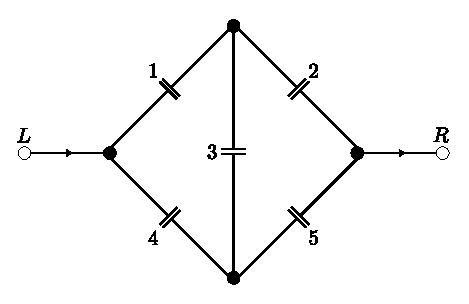
\includegraphics[width=\unitlength]{Fig3.11(a).eps}}%
  \end{picture}%
    \\
  \textbf{(a)}
  \end{center}
\endgroup%

\begingroup%
  \makeatletter%
  \providecommand\color[2][]{%
    \errmessage{(Inkscape) Color is used for the text in Inkscape, but the package 'color.sty' is not loaded}%
    \renewcommand\color[2][]{}%
  }%
  \providecommand\transparent[1]{%
    \errmessage{(Inkscape) Transparency is used (non-zero) for the text in Inkscape, but the package 'transparent.sty' is not loaded}%
    \renewcommand\transparent[1]{}%
  }%
  \providecommand\rotatebox[2]{#2}%
  \newcommand*\fsize{\dimexpr\f@size pt\relax}%
  \newcommand*\lineheight[1]{\fontsize{\fsize}{#1\fsize}\selectfont}%
  \ifx\svgwidth\undefined%
    \setlength{\unitlength}{288bp}%
    \ifx\svgscale\undefined%
      \relax%
    \else%
      \setlength{\unitlength}{\unitlength * \real{\svgscale}}%
    \fi%
  \else%
    \setlength{\unitlength}{\svgwidth}%
  \fi%
  \global\let\svgwidth\undefined%
  \global\let\svgscale\undefined%
  \makeatother%
  \begin{center}
  \begin{picture}(1,0.52499998)%
    \lineheight{1}%
    \setlength\tabcolsep{0pt}%
    \put(0,0){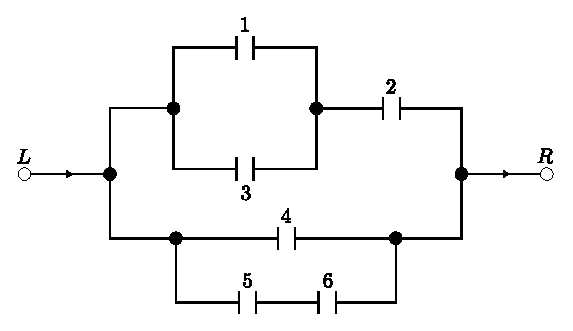
\includegraphics[width=\unitlength]{Fig3.11(b).eps}}%
  \end{picture}%
  \\
  \textbf{(b)}
  \end{center}
\endgroup%


\textbf{Note: Find the paths the current may take in the circuit, treat as finding the probability $P(\bigcup^n_{i=1} A_i)$ for $n$ paths, where $A_i$ is a path, and then apply the inclusion-exclusion principle.}

Let $A_i$ be the event of the current running through the $i$-th relay.

\textbf{(a)} The paths the current may take are $\{ 1, 2 \}, \{ 4, 5 \}, \{ 1, 3, 5 \}, \{ 4, 3, 2 \}$. Then the the objective is to calculate

\[ P(E) = P((A_1 \cap A_2) \cup (A_4 \cap A_5) \cup (A_1 \cap A_3 \cap A_5) \cup (A_4 \cap A_3 \cap A_2)) \]

Let $D1 = A_1 \cap A_2, D2 = A_4 \cap A_5, D3 = A_1 \cap A_3 \cap A_5, D4 = A_4 \cap A_3 \cap A_2$. Apply the inclusion-exclusion principle as follows,

\begin{align*}
P(E) &= \sum^4_{i = 1} P(D_i) - \sum^4_{i < j = 2} P(D_i \cap D_j) + \sum^4_{i < j < k = 3} P(D_i \cap D_j \cap D_k)  - P\Bigg(\bigcap^4_{i=1} D_i \Bigg) \\
&= p^2 + p^2 + p^3 + p^3 - p^4 - p^4 - p^4 - p^4 - p^4 - p^5 + p^5+ p^5+ p^5+ p^5- p^5 \\
&= \boxed{2p^2 + 2p^3 - 5p^4 + 2p^5}
\end{align*}

\textbf{(b)} The paths the current may take are $\{ 1, 2 \}, \{ 3, 2 \}, \{ 4 \}, \{ 5, 6\}$. Define $D1 = A_1 \cap A_2, D2 = A_3 \cap A_2, D3 = A_4, D4 = A_5 \cap A_6$. Then,

\begin{align*}
P(E) = P\Bigg( \bigcup^4_{i=1} D_i \Bigg) &= \sum^4_{i = 1} P(D_i) - \sum^4_{i < j = 2} P(D_i \cap D_j) + \sum^4_{i < j < k = 3} P(D_i \cap D_j \cap D_k)  - P\Bigg(\bigcap^4_{i=1} D_i \Bigg) \\
&= p^2 + p^2 + p + p^2 - p^3 - p^3 - p^3 - p^4 - p^4 - p^3 + p^4 + p^5 + p^5 + p^5 - p^6 \\
&= \boxed{p + 3p^2 - 4p^3 - p^4 + 3p^5 - p^6}
\end{align*}

%Question 3.21
\item  \begin{tcolorbox}[
  colback=Cerulean!5!white,
  colframe=Cerulean!75!black]
\textbf{Two machines, $\bm{A}$, $\bm{B}$, being operated independently, may have a number of breakdowns each day. Table 3.2 gives the probability distribution of breakdowns for each machine. Compute the following probabilities.}
\end{tcolorbox}

\begin{center}
\textbf{Table 3.2} \\
\textbf{ }\\
\renewcommand{\arraystretch}{3.5}
\begin{tabular}{c || c c c c c c c} 
 \hline
 Number of breakdowns & 0 & 1 & 2 & 3 & 4 & 5 & 6 \\
 \hline
$A$ & 0.1 & 0.2 & 0.3 & 0.2 & 0.09 & 0.07 & 0.04 \\
 \hline
$B$ & 0.3 & 0.1 & 0.1 & 0.1 & 0.1 & 0.15 & 0.15 \\
 \hline
\end{tabular}
\end{center}

	\begin{enumerate}
	%Question 3.21(a)
	\item  \begin{tcolorbox}[
	  colback=Cerulean!5!white,
	  colframe=Cerulean!75!black]
	\textbf{$\bm{A}$ and $\bm{B}$ have the same number of breakdowns.}
	\end{tcolorbox}
	
	Define $a_0, a_1, a_2, a_3, a_4, a_5, a_6$ as the events that both machines have $0, 1, 2, 3, 4, 5, 6$ breakdowns, respectively. Note that each of these events are mutually exclusive; namely, the machines cannot have two different numbers of breakdowns on the same day. Thus the probability simply is calculated as
	
	\begin{align*}
	P\Bigg( \bigcup^6_{i = 0} a_i \Bigg) &= \sum^6_{i = 0} P(a_i) \\
	&= (0.1)(0.3) + (0.2)(0.1) + (0.3)(0.1) + (0.2)(0.1) + (0.09)(0.1) + (0.07)(0.15) + (0.04)(0.15) \\
	&= \boxed{0.126}
	\end{align*}
	
	%Question 3.21(b)
	\item  \begin{tcolorbox}[
	  colback=Cerulean!5!white,
	  colframe=Cerulean!75!black]
	\textbf{The total number of breakdowns is less than 4; less than 5.}
	\end{tcolorbox}
	
	Let $P_A(i), P_B(j)$ be the probability that machines $A, B$ have $i, j$ breakdowns, respectively. We calculate
	
	\textbf{\bm{$\boxed{i + j < 4}$}}
	
	\begin{align*}
	P_{A,B}(i + j < 4) &= P_A(0) P_B(0) + P_A(0) P_B(1) + P_A(0) P_B(2) + P_A(0) P_B(3) + P_A(1) P_B(0) + P_A(1) P_B(1) \\
	&\quad + P_A(1) P_B(2) + P_A(2) P_B(0) + P_A(2) P_B(1) + P_A(3) P_B(0) \\
	&= (0.1)(0.3) + (0.1)(0.1) + (0.1)(0.1) + (0.1)(0.1) + (0.2)(0.3) + (0.2)(0.1) + (0.2)(0.1) \\ 
	&\quad+ (0.3)(0.3) + (0.3)(0.1) + (0.2)(0.3) \\
	&= \boxed{0.34}
	\end{align*}
	
	\textbf{\bm{$\boxed{i + j < 5}$}}

	\begin{align*}
	P_{A,B}(i + j < 5) &= P_A(0) P_B(0) + P_A(0) P_B(1) + P_A(0) P_B(2) + P_A(0) P_B(3) + P_A(0) P_B(4) + P_A(1) P_B(0) \\
	&\quad + P_A(1) P_B(1) + P_A(1) P_B(2) + P_A(1) P_B(3) + P_A(2) P_B(0) + P_A(2) P_B(1) + P_A(2) P_B(2)  \\
	&\quad + P_A(3) P_B(0) + P_A(3) P_B(1) + P_A(4) P_B(0) \\
	&= (0.1)(0.3) + (0.1)(0.1) + (0.1)(0.1) + (0.1)(0.1) + (0.1)(0.1) + (0.2)(0.3) + (0.2)(0.1) + (0.2)(0.1) \\ 
	&\quad+ (0.2)(0.1) + (0.3)(0.3) + (0.3)(0.1) + (0.3)(0.1) + (0.2)(0.3) + (0.2)(0.1) + (0.09)(0.3) \\
	&= \boxed{0.447}
	\end{align*}
	
	%Question 3.21(c)
	\item  \begin{tcolorbox}[
	  colback=Cerulean!5!white,
	  colframe=Cerulean!75!black]
	\textbf{$\bm{A}$ has more breakdowns than $\bm{B}$.}
	\end{tcolorbox}
	
	\begin{align*}
	P_{A,B} (i > j) &= P_A(1) P_B(0) + P_A(2) P_B(0) + P_A(2) P_B(1) + P_A(3) P_B(0) + P_A(3) P_B(1) + P_A(3) P_B(2) \\
	&\quad + P_A(4) P_B(0) + P_A(4) P_B(1) + P_A(4) P_B(2) + P_A(4) P_B(3) + P_A(5) P_B(0) + P_A(5) P_B(1) \\
	&\quad + P_A(5) P_B(2) + P_A(5) P_B(3) + P_A(5) P_B(4) + P_A(6) P_B(0) + P_A(6) P_B(1) + P_A(6) P_B(2) \\
	&\quad + P_A(6) P_B(3) + P_A(6) P_B(4) + P_A(6) P_B(5) \\
	&= (0.2)(0.3) + (0.3)(0.3) + (0.3)(0.1) + (0.2)(0.3) + (0.2)(0.1) + (0.2)(0.1) + (0.09)(0.3) + (0.09)(0.1) \\
	&\quad + (0.09)(0.1) + (0.09)(0.1) + (0.07)(0.3) + (0.07)(0.1) + (0.07)(0.1) + (0.07)(0.1) + (0.07)(0.1) \\
	&\quad + (0.04)(0.3) + (0.04)(0.1) + (0.04)(0.1) + (0.04)(0.1) + (0.04)(0.1) + (0.04)(0.15) \\
	&= \boxed{0.417}
	\end{align*}
	
	%Question 3.21(d)
	\item  \begin{tcolorbox}[
	  colback=Cerulean!5!white,
	  colframe=Cerulean!75!black]
	\textbf{$\bm{B}$ has twice as many breakdowns as $\bm{A}$.}
	\end{tcolorbox}
	
	\[ P_{A,B}(i = 2j) = P_A(1) P_B(2) + P_A(2) P_B(4) + P_A(3) P_B(6) = (0.2)(0.1) + (0.3)(0.1) + (0.2)(0.15) = \boxed{0.08} \]
	
	%Question 3.21(e)
	\item  \begin{tcolorbox}[
	  colback=Cerulean!5!white,
	  colframe=Cerulean!75!black]
	\textbf{$\bm{B}$ has 4 breakdowns, when it is known that $\bm{B}$ has at least 2 breakdowns.}
	\end{tcolorbox}
	
	We first observe that
	
	\[ P_{A,B} (j = 4 \ | \ j \geq 2) = \frac{P_{A,B} (j = 4, j \geq 2)}{P_{A,B} (j \geq 2)} = \frac{P_{A,B} (j = 4, j \geq 2)}{1 - P_{A,B}(j < 2)} \]
	
	And now we calculate the constituent terms:
	
	\begin{align*}
	P_{A,B}(j < 2) &= \sum^6_{i = 0} P_{A,B}(i, 0) + \sum^6_{i = 0} P_{A,B}(i, 1) \\
	&= (0.1)(0.3) + (0.2)(0.3) + (0.3)(0.3) + (0.2)(0.3) + (0.09)(0.3) + (0.07)(0.3) + (0.04)(0.3) \\
	&\quad + (0.1)(0.1) + (0.2)(0.1) + (0.3)(0.1) + (0.2)(0.1) + (0.09)(0.1) + (0.07)(0.1) + (0.04)(0.1) \\
	&= 0.4 \\
	\implies 1 - P_{A,B}(j < 2) &= 0.6 \\
	P_{A,B} (j = 4, j \geq 2) &= (0.1)(0.1) + (0.2)(0.1) + (0.3)(0.1) + (0.2)(0.1) + (0.09)(0.1) + (0.07)(0.1) + (0.04)(0.1) \\
	&= 0.1 \\
	\implies \frac{P_{A,B} (j = 4, j \geq 2)}{1 - P_{A,B}(j < 2)} &= 0.1/0.6 = \boxed{0.167}
	\end{align*}
	
	%Question 3.21(f)
	\item  \begin{tcolorbox}[
	  colback=Cerulean!5!white,
	  colframe=Cerulean!75!black]
	\textbf{The minimum number of breakdowns of the two machines is 3; is less than 3.}
	\end{tcolorbox}
	
	\textbf{$\boxed{\bm{\min(i+j) = 3}}$}
	
	\begin{align*}
	P_{A,B} (i + j \geq 3) &= 1 - P_{A,B} (i + j < 3) \\
	&= 1 - [P_A(0)P_B(2) + P_A(1)P_B(1) + P_A(2)P_B(1) + P_A(0)P_B(1) + P_A(1)P_B(0) + P_A(0)P_B(0)] \\
	&= 1 - [(0.1)(0.1) + (0.2)(0.1) + (0.3)(0.3) + (0.1)(0.1) + (0.2)(0.3) + (0.1)(0.3)] \\
	&= \boxed{0.78}
	\end{align*}
	
	\textbf{$\boxed{\bm{\min(i+j) < 3}}$}

	\begin{align*}
	P_{A,B} (i + j \geq 2) &= 1 - P_{A,B} (i + j < 2) \\
	&= 1 - [P_A(0)P_B(0) + P_A(0)P_B(1) + P_A(1)P_B(0)] \\
	&= 1 - [(0.1)(0.3) + (0.1)(0.1) + (0.2)(0.3) ] \\
	&= \boxed{0.9} \\
	P_{A,B} (i + j \geq 1) &= 1 - P_{A,B} (i + j < 1) \\
	&= 1 - P_A(0)P_B(0) \\
	&= 1 - (0.1)(0.3) \\
	&= \boxed{0.97} \\
	P_{A,B} (i + j \geq 0) &= 1 - P_{A,B} (i + j < 0) \\	
	&= \boxed{1}
	\end{align*}
	
	%Question 3.21(g)
	\item  \begin{tcolorbox}[
	  colback=Cerulean!5!white,
	  colframe=Cerulean!75!black]
	\textbf{The maximum number of breakdowns of the machines is 3; is more than 3.}
	\end{tcolorbox}
	
	\textbf{$\boxed{\bm{\max(i+j) = 3}}$}
	
	\begin{align*}
	P_{A,B} (i + j \leq 3) &= P_A(0)P_B(2) + P_A(1)P_B(1) + P_A(2)P_B(1) + P_A(0)P_B(1) + P_A(1)P_B(0) + P_A(0)P_B(0) \\
	&\quad + P_A(0)P_B(3) + P_A(2)P_B(1) + P_A(1)P_B(2) + P_A(3)P_B(0) \\
	&= (0.1)(0.1) + (0.2)(0.1) + (0.3)(0.3) + (0.1)(0.1) + (0.2)(0.3) + (0.1)(0.3) + (0.1)(0.1) \\ 
	&\quad + (0.3)(0.1) + (0.2)(0.1) + (0.2)(0.3) \\
	&= \boxed{0.34}
	\end{align*}
	
	\textbf{$\boxed{\bm{\max(i+j) > 3}}$}
	
	\begin{align*}
	P_{A,B} (i + j \leq 4) &= P_A(0)P_B(3) + P_A(1)P_B(2) + P_A(2)P_B(1) + P_A(3)P_B(0) + P_A(2)P_B(0) \\
	&\quad + P_A(0)P_B(2) + P_A(1)P_B(1) + P_A(1)P_B(0) + P_A(0)P_B(1) + P_A(0)P_B(0) + P_A(0)P_B(4) \\
	&\quad + P_A(1)P_B(3) + P_A(2)P_B(2) + P_A(3)P_B(1) + P_A(4)P_B(0) \\
	&= (0.1)(0.1) + (0.2)(0.1) + (0.3)(0.1) + (0.2)(0.3) + (0.3)(0.3) + (0.1)(0.1) + (0.2)(0.1) \\
	&\quad + (0.2)(0.3) + (0.1)(0.1) + (0.1)(0.3) + (0.1)(0.1) + (0.2)(0.1) + (0.3)(0.1) \\
	&\quad + (0.2)(0.1) + (0.09)(0.3) \\
	&= \boxed{0.447} \\
	P_{A,B} (i + j \leq 5) &= P_{A,B} (i + j \leq 4) + P_A (0) P_B (5) + P_A (1) P_B (4) + P_A (2) P_B (3) + P_A (3) P_B (2) \\
	& + P_A (4) P_B (1) + P_A (5) P_B (0) \\
	&= 0.447 + (0.1)(0.15) + (0.2)(0.1) + (0.3)(0.1) + (0.2)(0.1) + (0.09)(0.1) + (0.07)(0.3) \\
	&= \boxed{0.562} \\
	P_{A,B} (i + j \leq 6) &= P_{A,B} (i + j \leq 5) + P_A (0) P_B (6) + P_A (1) P_B (5) + P_A (2) P_B (4) + P_A (3) P_B (3) \\
	&\quad + P_A (4) P_B (2) + P_A (5) P_B (1) + P_A(6) P_B(0) \\
	&= 0.562 + (0.1)(0.15) + (0.2)(0.15) + (0.3)(0.1) + (0.2)(0.1) \\
	&\quad + (0.09)(0.1) + (0.07)(0.1) + (0.04)(0.3) \\
	&= \boxed{0.685} \\
	P_{A,B} (i + j \leq 7) &= P_{A,B} (i + j \leq 6) + P_A (1) P_B (6) + P_A (2) P_B (5) + P_A (3) P_B (4) + P_A (4) P_B (3) \\
	&\quad + P_A (5) P_B (2) + P_A (6) P_B (1) \\
	&= 0.685 + (0.2)(0.15) + (0.3)(0.15) + (0.2)(0.1) + (0.09)(0.1) + (0.07)(0.1) + (0.04)(0.1) \\
	&= \boxed{0.8} \\
	P_{A,B} (i + j \leq 8) &= P_{A,B} (i + j \leq 7) + P_A (2) P_B (6) + P_A (3) P_B (5) + P_A (4) P_B (4) + P_A (5) P_B (3) + P_A (6) P_B (2) \\
	&= 0.8 + (0.3)(0.15) + (0.2)(0.15) + (0.09)(0.1) + (0.07)(0.1) + (0.04)(0.1) \\
	&= \boxed{0.895} \\
	P_{A,B} (i + j \leq 9) &= P_{A,B} (i + j \leq 8) + P_A (3) P_B (6) + P_A (4) P_B (5) + P_A (5) P_B (4) + P_A (6) P_B (3) \\
	&= 0.895 + (0.2)(0.15) + (0.09)(0.15) + (0.07)(0.1) + (0.04)(0.1) \\
	&= \boxed{0.9495} \\
	P_{A,B} (i + j \leq 10) &= P_{A,B} (i + j \leq 9) + P_A (4) P_B (6) + P_A (5) P_B (5) + P_A (6) P_B (4) \\
	&= 0.9495 + (0.09)(0.15) + (0.07)(0.15) + (0.04)(0.1) \\
	&= \boxed{0.9775} \\
	P_{A,B} (i + j \leq 11) &= P_{A,B} (i + j \leq 10) + P_A (5) P_B (6) + P_A (6) P_B (5) \\
	&= 0.9775 + (0.07)(0.15) + (0.04)(0.15) \\
	&= \boxed{0.994} \\
	P_{A,B} (i + j \leq 12) &= P_{A,B} (i + j \leq 11) + P_A (6) P_B (6) \\
	&= 0.994 + (0.04)(0.15) \\
	&= \boxed{1}
	\end{align*}
	
	\end{enumerate}

\newpage
%Question 3.22
\item  \begin{tcolorbox}[
  colback=Cerulean!5!white,
  colframe=Cerulean!75!black]
\textbf{By verifying Eq. (3.2), show that for fixed $\bm{A}$, $\bm{P(B | A)}$ satisfies the various postulates for probability.}
\end{tcolorbox}

\textbf{(1)} Since $P(B | A) = \frac{P(A \cap B)}{P(A)}$ and $A \cap B \subset A \implies P(A \cap B) \leq P(A)$, it follows that $0 \leq P(B | A) \leq 1$.

\textbf{(2)} $P(S | A) = \frac{P(S \cap A)}{P(A)} = \frac{P(A)}{P(A)} = 1$

\textbf{(3)} If $B_1 \cap B_2 = \emptyset$, then $P(B_1 \cup B_2 | A) = \frac{P( (B_1 \cup B_2 ) \cap A)}{P(A)} = \frac{P((B_1 \cap A) \cup (B_2 \cap A))}{P(A)} = \frac{P(B_1 \cap A)}{P(A)} + \frac{P(B_2 \cap A)}{P(A)} = P(B_1 | A) + P(B_2 | A)$

\textbf{(4)} By assumption, $B_i \cap B_j = \emptyset \ \forall i \neq j$. Then $(B_i \cap A) \cap (B_j \cap A) = \emptyset \ \forall i \neq j$. Then applying (4) from the original definition of probability, $P(\bigcup^\infty_{i = 1} B_i | A) = \sum^\infty_{i = 1} P(B_i | A)$.

%Question 3.23
\item  \begin{tcolorbox}[
  colback=Cerulean!5!white,
  colframe=Cerulean!75!black]
\textbf{If each element of a second order determinant is either zero or one, what is the probability that the value of the determinant is positive? (Assume that the individual entries of the determinant are chosen independently, each value being assumed with probability 1/2.)}
\end{tcolorbox}

A second-order determinant is of the form $   \begin{vmatrix} % or pmatrix or bmatrix or Bmatrix or ...
      a_1 & a_2 \\
      a_3 & a_4 \\
   \end{vmatrix}$. There are $2^4$ arrangements if each element is either a zero or one. The determinant is calculated as $a_1 a_4 - a_2 a_3$. Defining positive as any number strictly greater than zero, the only permissible value of the determinant is one. Therefore, we need only count the combinations such that $a_1 a_4 = 1$ and $a_2 a_3 = 0$. In the first case, we must have $a_1 = a_4 = 1$. In the second, we may have either $a_2 = 1, a_3 = 0$; $a_2 = 0, a_3 = 1$; or $a_2 = a_3 = 0$. Each possible set of values the determinant takes on has a $1/16$ chance of occurring. Since each of these outcomes is mutually exclusive (we cannot have an element be both one and zero), we need only add the probabilities of the three outcomes and get $\boxed{3/16}$.
   
%Question 3.24
\item  \begin{tcolorbox}[
  colback=Cerulean!5!white,
  colframe=Cerulean!75!black]
\textbf{Show that the multiplication theorem $\bm{P(A \cap B) = P(A | B) P(B)}$, established for two events, may be generalized to three events as follows: $\bm{P(A \cap B \cap C) = P(A | B \cap C) P(B | C) P(C)}$.}
\end{tcolorbox}

\begin{proof} Obseve that $P(A \cap (B \cap C)) = P(A | B \cap C) P(B \cap C) = P(A | B \cap C) P(B | C) P(C)$.
\end{proof}

%Question 3.25
\item  \begin{tcolorbox}[
  colback=Cerulean!5!white,
  colframe=Cerulean!75!black]
\textbf{An electronic assembly consists of two subsystems, say $\bm{A}$ and $\bm{B}$. From previous testing procedures, the following probabilities are assumed to be known: $\bm{P(A \text{ fails}) = 0.20, P(B \text{ fails alone}) = 0.15, P(A \text{ and } B \text{ fail}) = 0.15}$. Evaluate the following probabilities.}
\end{tcolorbox}

	\begin{enumerate}
	%Question 3.25(a)
	\item  \begin{tcolorbox}[
	  colback=Cerulean!5!white,
	  colframe=Cerulean!75!black]
	\textbf{$\bm{P(A \text{ fails } | B \text{ has failed})}$,}
	\end{tcolorbox}
	
	Observe that $P(B \text{ fails}) = P(B \text{ fails alone or } A \text{ and } B \text{ fail})$. Then this gives us $P(B \text{ fails alone}) + P(A \text{ and } B \text{ fail}) - P(B \text{ fails alone and } A \text{ and } B \text{ fail}) = 0.15 + 0.15 = 0.30$. Then $P(A \text{ fails } | B \text{ has failed}) = \frac{P(A \text{ fails } \cap B \text{ has failed})}{P(B \text{ fails})} = \frac{0.15}{0.30} = \boxed{0.5}$.
	
	%Question 3.25(b)
	\item  \begin{tcolorbox}[
	  colback=Cerulean!5!white,
	  colframe=Cerulean!75!black]
	\textbf{$\bm{P(A \text{ fails alone})}$.}
	\end{tcolorbox}
	
	Observe that $P(A \text{ fails}) = P(A \text{ fails alone}) + P(A \text{ and } B \text{ fail}) - P(A \text{ fails alone and } A \text{ and } B \text{ fail})$. Then $P(A \text{ fails alone}) = P(A \text{ fails}) - P(A \text{ and } B \text{ fail}) = 0.20 - 0.15 = \boxed{0.05}$.
	\end{enumerate}

\newpage
%Question 3.26
\item  \begin{tcolorbox}[
  colback=Cerulean!5!white,
  colframe=Cerulean!75!black]
\textbf{Finish the analysis of the example given in Section 3.2 by deciding which of the types of candy jar, $\bm{A}$ or $\bm{B}$, is involved, based on the evidence of two pieces of candy which were sampled.}
\end{tcolorbox}

% Set the overall layout of the tree
\tikzstyle{level 1}=[level distance=3.5cm, sibling distance=3.5cm]
\tikzstyle{level 2}=[level distance=3.5cm, sibling distance=2cm]

% Define styles for bags and leafs
\tikzstyle{bag} = [circle, minimum width=3pt,fill, inner sep=0pt]
\tikzstyle{end} = [circle, minimum width=3pt,fill, inner sep=0pt]

% The sloped option gives rotated edge labels. Personally
% I find sloped labels a bit difficult to read. Remove the sloped options
% to get horizontal labels. 
\begin{center}
\begin{tikzpicture}[level 1/.style={sibling distance=25mm},
   level 2/.style={sibling distance=7mm}, grow = right]
\node[bag] {}
    child {
        node[bag] {}        
            child {
                node[end, label=right:
                    {$S_O, S_O$}] {}
                edge from parent
                node[above] {}
                node[below]  {}
            }
            child {
                node[end, label=right:
                    {$S_W, S_O \text{ or } S_O, S_W$}] {}
                edge from parent
                node[above] {}
                node[below]  {}
            }
            child {
                node[end, label=right:
                    {$S_W, S_W$}] {}
                edge from parent
                node[above] {}
                node[below]  {}
            }
            edge from parent 
            node[above] {}
            node[below]  {$B$}
    }
    child {
        node[bag] {}        
        child {
                node[end, label=right:
                    {$S_O, S_O$}] {}
                edge from parent
                node[above] {}
                node[below]  {}
            }
            child {
                node[end, label=right:
                    {$S_W, S_O \text{ or } S_O, S_W$}] {}
                edge from parent
                node[above] {}
                node[below]  {}
            }
            child {
                node[end, label=right:
                    {$S_W, S_W$}] {}
                edge from parent
                node[above] {}
                node[below]  {}
            }
        edge from parent         
            node[above] {$A$}
            node[below]  {}
    };
\end{tikzpicture}
\end{center}

\textbf{Meyer, 2nd ed. page 40:} \say{Suppose that a large number of containers of candy are made up of two types, say $A$ and $B$. Type $A$ contains 70 percent sweet ($S_W$) and 30 percent sour ($S_O$) ones while for type $B$ these percentages are reversed. Furthermore, suppose that 60 percent of all candy jars are of type $A$ while the remainder are of type $B$.}

Define the events $S^2_W$ for choosing two sweets, $S^2_O$ for choosing two sours, $S_W S_O$ for choosing a sweet and a sour, and $S_O S_W$ for choosing a sour and a sweet. Make the additional assumption that the candy containers have so much candy that we can approximate picking one candy after another as independent events (we do this because the author does not actually give a number for how many candies there are per container). Then using the following definition:

\begin{defn} If $A, B$ given $C$ are conditionally independent events, then 

\[ P(A, B | C) = P(A | C) P(B | C) \]
\end{defn}

It follows that $P(S^2_W | A) = P(S_W | A) P(S_W | A)$, and analogously for the other pairs of candies. We calculate:

\begin{align*}
P(A | S^2_W) &= \frac{P(S^2_W | A) P(A) }{P(S^2_W | A) P(A) + P(S^2_W | B) P(B)} \\
&= \frac{0.7^2 \cdot 0.6 }{ 0.7^2 \cdot 0.6 + 0.3^2 \cdot 0.4} \\
&= \boxed{0.891} \\
P(B | S^2_W) &= \frac{P(S^2_W | B) P(B) }{P(S^2_W | A) P(A) + P(S^2_W | B) P(B)} \\
&= \frac{0.3^2 \cdot 0.4 }{ 0.7^2 \cdot 0.6 + 0.3^2 \cdot 0.4} \\
&= \boxed{0.109} \\
P(A | S^2_O) &= \frac{P(S^2_O | A) P(A) }{P(S^2_O | A) P(A) + P(S^2_O | B) P(B)} \\
&= \frac{0.3^2 \cdot 0.6 }{ 0.3^2 \cdot 0.6 + 0.7^2 \cdot 0.4} \\
&= \boxed{0.216} \\
P(B | S^2_O) &= \frac{P(S^2_O | B) P(B) }{P(S^2_O | A) P(A) + P(S^2_O | B) P(B)} \\
&= \frac{0.7^2 \cdot 0.4 }{ 0.3^2 \cdot 0.6 + 0.7^2 \cdot 0.4} \\
&= \boxed{0.784} \\
P(A | S_W S_O \cup S_O S_W) &= \frac{P(S_W S_O \cup S_O S_W | A) P(A)}{P(S_W S_O \cup S_O S_W | A) P(A) + P(S_W S_O \cup S_O S_W | B) P(B)} \\
&= \frac{ [ P(S_W S_O | A) + P(S_O S_W | A) ] P(A)}{ [ P(S_W S_O | A) + P(S_O S_W | A) ] P(A) + [ P(S_W S_O | B) + P(S_O S_W | B) ] P(B)} \\
&= \frac{ (0.7 \cdot 0.3 + 0.3 \cdot 0.7) \cdot 0.6}{ (0.7 \cdot 0.3 + 0.3 \cdot 0.7) \cdot 0.6 + (0.3 \cdot 0.7 + 0.7 \cdot 0.3) \cdot 0.4 } \\
&= \boxed{0.6} \\
P(B | S_W S_O \cup S_O S_W) &= \frac{P(S_W S_O \cup S_O S_W | B) P(B)}{P(S_W S_O \cup S_O S_W | A) P(A) + P(S_W S_O \cup S_O S_W | B) P(B)} \\
&= \frac{ [ P(S_W S_O | B) + P(S_O S_W | B) ] P(B)}{ [ P(S_W S_O | A) + P(S_O S_W | A) ] P(A) + [ P(S_W S_O | B) + P(S_O S_W | B) ] P(B)} \\
&= \frac{ (0.3 \cdot 0.7 + 0.7 \cdot 0.3) \cdot 0.4}{ (0.7 \cdot 0.3 + 0.3 \cdot 0.7) \cdot 0.6 + (0.3 \cdot 0.7 + 0.7 \cdot 0.3) \cdot 0.4 } \\
&= \boxed{0.4}
\end{align*}

%Question 3.27
\item  \begin{tcolorbox}[
  colback=Cerulean!5!white,
  colframe=Cerulean!75!black]
\textbf{Whenever an experiment is performed, the occurrence of a particular event $\bm{A}$ equals 0.2. The experiment is repeated, independently, until $\bm{A}$ occurs. Compute the probability that it will be necessary to carry out a fourth experiment.}
\end{tcolorbox}

Equivalently, we want to find the probability that $A$ has not occurred in the first, second, and third experiments. The probability of $A$ not occurring is 0.8. By premise and by application of problem 3.19, it is 0.8 for each iteration. Appealing once more to event independence, the probability of $A$ failing to occur after three iterations is $0.8^3 = \boxed{0.512}$.

%Question 3.28
\item  \begin{tcolorbox}[
  colback=Cerulean!5!white,
  colframe=Cerulean!75!black]
\textbf{Suppose that a mechanism has $\bm{N}$ tubes, all of which are needed for its functioning. To locate a malfunctioning tube one replaces each tube, successively, with a new one. Compute the probability that it will be necessary to check $\bm{N}$ tubes if the (constant) probability is $\bm{p}$ that a tube is out of order.}
\end{tcolorbox}

Assume that only one of the tubes in the system is malfunctioning, and it happens to be the $N$-th tube. To reach the $N$-th tube, the inspector must begin with the first, and replace tubes $1, 2, ..., N-1$ until reaching the $N$-th. To successively check $N$ tubes one after another, it must be the case that all of the tubes up to the $N$-th are in working order. Then the probability of checking $N$ tubes is $\boxed{(1-p)^{N-1} p}$.

%Question 3.29
\item  \begin{tcolorbox}[
  colback=Cerulean!5!white,
  colframe=Cerulean!75!black]
\textbf{Prove: If $\bm{P(A | B) > P(A)}$ then $\bm{P(B | A) > P(B)}$.}
\end{tcolorbox}

\begin{proof}
By premise, $\frac{P(A \cap B)}{P(B)} > P(A)$. Assuming $P(A), P(B) > 0$, then $\frac{P(A \cap B)}{P(A)}  = \frac{P(B \cap A)}{P(A)} = P(B | A) > P(B)$. 
\end{proof}

%Question 3.30
\item  \begin{tcolorbox}[
  colback=Cerulean!5!white,
  colframe=Cerulean!75!black]
\textbf{A vacuum tube may come from any one of three manufacturers with probabilities $\bm{p_1 = 0.25, p_2 = 0.50}$, and $\bm{p_3 = 0.25}$. The probabilities that the tube will function properly during a specified period of time equal 0.1, 0.2, and 0.4, respectively, for the three manufacturers. Compute the probability that a randomly chosen tube will function for the specified period of time.}
\end{tcolorbox}

Let $A_i$ denote the $i$-th manufacturer the tube came from, and $W$ be the event that the tube works. Then the desired probability is $P(\bigcup^3_{i=1} (A_i \cap W))$. Note that each of these events is mutually exclusive, as we are only choosing one tube, so $P(\bigcup^3_{i=1} (A_i \cap W)) = \sum^3_{i = 1} P(A_i \cap W)$. For each $i$, $P(A_i \cap W) = P(W | A_i) P(A_i)$, so we equivalently write  $P(\bigcup^3_{i=1} (A_i \cap W)) = \sum^3_{i = 1} P(W | A_i) P(A_i)$. Calculating yields $0.25 \cdot 0.1 + 0.5 \cdot 0.2 + 0.25 \cdot 0.4 = \boxed{0.225}$.

%Question 3.31
\item  \begin{tcolorbox}[
  colback=Cerulean!5!white,
  colframe=Cerulean!75!black]
\textbf{An electrical system consists of two switches of type $\bm{A}$, one of type $\bm{B}$, and four of type $\bm{C}$, connected as in Fig. 3.12. Compute the probability that a break in the circuit cannot be eliminated with key $\bm{K}$ if the switches $\bm{A, B}$, and $\bm{C}$ are open (i.e., out of order) with probabilities 0.3, 0.4, and 0.2, respectively, and if they operate independently.}
\end{tcolorbox}

\begingroup%
  \makeatletter%
  \providecommand\color[2][]{%
    \errmessage{(Inkscape) Color is used for the text in Inkscape, but the package 'color.sty' is not loaded}%
    \renewcommand\color[2][]{}%
  }%
  \providecommand\transparent[1]{%
    \errmessage{(Inkscape) Transparency is used (non-zero) for the text in Inkscape, but the package 'transparent.sty' is not loaded}%
    \renewcommand\transparent[1]{}%
  }%
  \providecommand\rotatebox[2]{#2}%
  \newcommand*\fsize{\dimexpr\f@size pt\relax}%
  \newcommand*\lineheight[1]{\fontsize{\fsize}{#1\fsize}\selectfont}%
  \ifx\svgwidth\undefined%
    \setlength{\unitlength}{360bp}%
    \ifx\svgscale\undefined%
      \relax%
    \else%
      \setlength{\unitlength}{\unitlength * \real{\svgscale}}%
    \fi%
  \else%
    \setlength{\unitlength}{\svgwidth}%
  \fi%
  \global\let\svgwidth\undefined%
  \global\let\svgscale\undefined%
  \makeatother%
  \begin{center}
  \begin{picture}(1,0.6)%
    \lineheight{1}%
    \setlength\tabcolsep{0pt}%
    \put(0,0){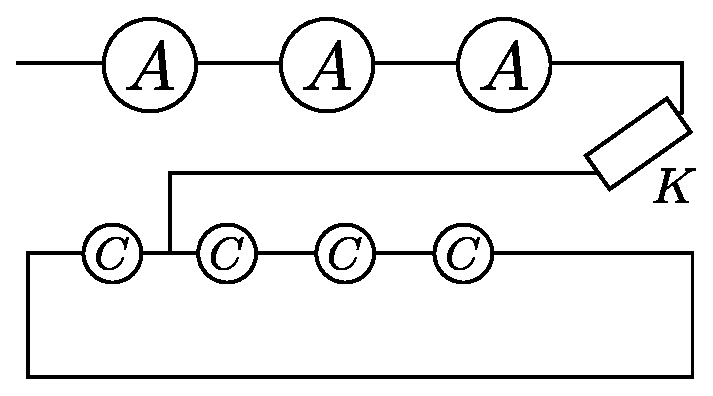
\includegraphics[width=\unitlength]{Fig3.12.eps}}%
  \end{picture}%
  \end{center}
\endgroup%


$(0.3)^2 (0.4) (0.2)^2 = \boxed{5.76 \cdot 10^{-5}}$

%Question 3.32
\item  \begin{tcolorbox}[
  colback=Cerulean!5!white,
  colframe=Cerulean!75!black]
\textbf{The probability that a system becomes overloaded is 0.4 during each run of an experiment. Compute the probability that the system will cease functioning in three independent trials of the experiment if the probabilities of failure in 1, 2, or 3 trials equal 0.2, 0.5, and 0.8, respectively.}
\end{tcolorbox}

Question wording is not comprehensible.

%Question 3.33
\item  \begin{tcolorbox}[
  colback=Cerulean!5!white,
  colframe=Cerulean!75!black]
\textbf{Four radio signals are emitted successfully. If the reception of any one signal is independent of the reception of another and if these probabilities are 0.1, 0.2, 0.3, and 0.4, respectively, compute the probability that $\bm{k}$ signals will be received for $\bm{k = 0, 1, 2, 3, 4}$.}
\end{tcolorbox}

Define $A_i$ as the reception of the $i$-th signal.

$\bm{k = 0}:$ Equivalently, calculate $P(\bigcap^4_{i=1} \neg A_i) = \Pi^4_{i = 1} (1 - P(A_i)) = 0.9 \cdot 0.8 \cdot 0.7 \cdot 0.6 = \boxed{0.3024}$.

$\bm{k = 1}:$ The event $A_j \cap ( \bigcap^4_{i \neq j} \neg A_i )$ is only the $j$-th signal and NOT the others is received. Each such event is mutually exclusive.

\begin{align*}
&P\Bigg( \bigcup^4_{j = 1} [ A_j \cap ( \bigcap^4_{i \neq j} \neg A_i ) ] \Bigg) \\
&= (0.1)(0.8)(0.7)(0.6) + (0.9)(0.2)(0.7)(0.6) + (0.9)(0.8)(0.3)(0.6) + (0.9)(0.8)(0.7)(0.4) = \boxed{0.4404}
\end{align*}

$\bm{k = 2}:$ 
\begin{align*}
&P\Bigg( \bigcup^4_{i < j = 2} [ (A_i \cap A_j) \cap ( \bigcap^4_{k \neq i, j} \neg A_k) ] \Bigg) \\
&= (0.1)(0.2)(0.7)(0.6) + (0.1)(0.8)(0.3)(0.6) + (0.9)(0.2)(0.3)(0.6) + (0.1)(0.8)(0.7)(0.4) \\
&\quad + (0.9)(0.2)(0.7)(0.4) + (0.9)(0.8)(0.3)(0.4) = \boxed{0.2144}
\end{align*}

$\bm{k = 3}:$ For $l \neq i, j, k$:

\begin{align*}
&P\Bigg( \bigcup^4_{i < j < k = 3} (A_i \cap A_j \cap A_k \cap \neg A_l) \Bigg) \\
&= (0.1)(0.2)(0.3)(0.6) + (0.1)(0.2)(0.7)(0.4) + (0.1)(0.8)(0.3)(0.4) + (0.9)(0.2)(0.3)(0.4) = \boxed{0.0404}
\end{align*}

$\bm{k = 4}:$ $P(\bigcap^4_{i=1} A_i) = \Pi^4_{i = 1} P(A_i) = 0.1 \cdot 0.2 \cdot 0.3 \cdot 0.4 = \boxed{0.0024}$.

Observe that the probabilities of each case all sum to 1, as expected as the constituent $k$'s are mutually exclusive partitions of the sample space.

%Question 3.34
\item  \begin{tcolorbox}[
  colback=Cerulean!5!white,
  colframe=Cerulean!75!black]
\textbf{The following (somewhat simple-minded) weather forecasting is used by an amateur forecaster. Each day is classified as ``dry'' or ``wet'' and the probability that any given day is the same as the preceding one is assumed to be a constant $\bm{p \ (0 < p < 1)}$. Based on past records, it is supposed that January 1 has a probability of $\bm{\beta}$ of being ``dry.'' Letting $\bm{\beta_n =}$ probability (the $\bm{n}$th day of the year is ``dry''), obtain an expression for $\bm{\beta_n}$ in terms of $\bm{\beta}$ and $\bm{p}$. Also evaluate $\bm{\lim_{n \rightarrow \infty} \beta_n}$ and interpret your result.}
\end{tcolorbox}

The chief insight here is in the conceptual set up of the problem. By premise, on the first day of the year, there is probability $\beta$ of a dry day. Therefore the probability of a wet day is $1 - \beta$. 

The other pertinent fact is that each day has a $p$ probability of having the same weather as the previous day. Therefore, we can calculate the probability of the following day having dry weather as follows: either the first day can be dry and the second day has the same weather as the first, or the first day is wet, and the second day does not have the same weather as the first. Importantly, these are mutually exclusive events; the first day cannot have dry and wet weather (by our simplistic assumption). Then we can write:

   \begin{align*}
   P &\begin{pmatrix} % or pmatrix or bmatrix or Bmatrix or ...
      \text{Second day same as first day AND first day is dry}  \\
      \text{OR}  \\
      \text{Second day not same as first day AND first day is wet} \\
   \end{pmatrix} \\
   &= P(\text{Second day same as first day AND first day is dry}) \\
   &\quad + P( \text{Second day not same as first day AND first day is wet})
   \end{align*}
   
   Define the event $D_i$ as the probability that the weather on the $i$-th day is dry. Assuming that the weather of one day is independent of all other days, we can write as the probability of dry weather for the second day:
   
   \[ P(D_2) = p \beta_1 + (1-p)(1 - \beta_1) \]
   
   And we proceed so on and so forth such that $P(D_{n}) = p \cdot P(D_{n-1}) + (1-p) \cdot (1 - P(D_{n-1}))$. Then calculating $P(D_3)$ yields:
   
   \begin{align*}
   P(D_{3}) &= p \cdot P(D_{2}) + (1-p) \cdot (1 - P(D_{2})) \\
   &= p(p \beta_1 + (1-p)(1 - \beta_1)) + (1-p) (1 - (p \beta_1 + (1-p)(1 - \beta_1)))
   \end{align*}
   
   With some work of algebra, it can be shown that this reduces to:
   
   \[ P(D_3) = (2p-1)(p \beta_1 + (1-p)(1 - \beta_1)) + (1-p) \]
   
   And similarly, the probability for dry weather on the fourth and fifth days is:
   
   \begin{align*}
   P(D_4) &= (2p-1)^2 (p \beta_1 + (1-p)(1 - \beta_1)) + 2p(1-p) \\
   P(D_5) &= (2p-1)^3 (p \beta_1 + (1-p)(1 - \beta_1)) + (4p^2 - 2p + 1)(1-p)
   \end{align*}
   
   Although there is some regularity in the first term, the second one seems to elude a closed-form expression. Nor is it readily apparent what the limiting tendency is for increasing $n$. Returning to the $P(D_2)$ case, however, we can employ an algebraic trick to rewrite the expression as:
   
   \begin{align*}
   P(D_2) &= p \beta_1 + (1-p)(1 - \beta_1) \\
   &= p \beta_1 + 1 - \beta_1 - p + p \beta_1 \\
   &= 2p \beta_1 - \beta_1 - p + 1/2 + 1/2 \\
   &= (2p - 1)(\beta_1 - 1/2) + 1/2
   \end{align*}
   
   As we calculate successive $P(D_i)$ using this new form, we find a wonderful pattern emerging:
   
   \begin{align*}
   P(D_3) &= (2p - 1)^2 (\beta_1 - 1/2) + 1/2 \\
   P(D_4) &= (2p - 1)^3 (\beta_1 - 1/2) + 1/2 \\
   P(D_5) &= (2p - 1)^4 (\beta_1 - 1/2) + 1/2 \\
   &\vdots \\
   P(D_n) &= (2p - 1)^{n-1} (\beta_1 - 1/2) + 1/2
   \end{align*}
   
   And indeed, $\boxed{ \beta_n = P(D_n) = (2p - 1)^{n-1} (\beta_1 - 1/2) + 1/2}$ is our desired expression. To prove it, induct on $n$. Suppose it is true for $n-1$ days. Then:
   
   \begin{align*}
   P(D_n) &= p( (2p - 1)^{(n-1)-1} (\beta_1 - 1/2) + 1/2 ) + (1-p) \cdot (1 - ( (2p - 1)^{(n-1) -1} (\beta_1 - 1/2) + 1/2 )) \\
   &= p (2p - 1)^{(n-1)-1} (\beta_1 - 1/2) + p/2 + (1-p) - (1-p) (2p - 1)^{(n-1) -1} (\beta_1 - 1/2) - (1-p)/2 \\
   &= (2p - 1)^{n-1} (\beta_1 - 1/2) + p/2 + (1-p ) - (1-p)/2 \\
   &= (2p - 1)^{n-1} (\beta_1 - 1/2) + 1/2
   \end{align*}
   
   To calculate the limit:
   
   \[ \lim_{n \rightarrow \infty} [ (2p - 1)^{n-1} (\beta_1 - 1/2) + 1/2 ]  \]
   
   It must be deduced how $\lim_{n \rightarrow \infty} (2p - 1)^{n-1}$ is evaluated. By premise, $0 < p < 1$. Then $0 < 2p < 2$, implying $-1 < 2p - 1 < 1$, finally implying $|2p - 1| < 1$. Therefore, $\lim_{n \rightarrow \infty} (2p - 1)^{n-1} = 0$, and $\lim_{n \rightarrow \infty} [ (2p - 1)^{n-1} (\beta_1 - 1/2) + 1/2 ] = \boxed{1/2}$.

%Question 3.35
\item  \begin{tcolorbox}[
  colback=Cerulean!5!white,
  colframe=Cerulean!75!black]
\textbf{Three newspapers, $\bm{A, B,}$ and $\bm{C}$, are published in a city and a recent survey of readers indicates the following: 20 percent read $\bm{A}$, 16 percent read $\bm{B}$, 14 percent read $\bm{C}$, 8 percent read $\bm{A}$ and $\bm{B}$, 5 percent read $\bm{A}$ and $\bm{C}$, 2 percent read $\bm{A, B,}$ and $\bm{C}$, and 4 percent read $\bm{B}$ and $\bm{C}$. For one adult chosen at random, compute the probability that (a) he reads none of the papers (b) he reads exactly one of the papers (c) he reads at least $\bm{A}$ and $\bm{B}$ if it is known that he reads at least one of the papers published.}
\end{tcolorbox}

Define $A_i$ as the event of reading the $i$-th newspaper, where $i = 1, 2, 3$ corresponds to reading newspapers $A, B$, and $C$, respectively.

\textbf{(a)} 
\begin{align*}
P\Bigg( \bigcap^3_{i = 1} \neg A_i \Bigg) &= 1 - P \Bigg( \bigcup^3_{i = 1} A_i \Bigg) \\
&= 1 - (0.2 + 0.16 + 0.14 - 0.08 - 0.05 - 0.04 + 0.02) = \boxed{0.65}
\end{align*}

\textbf{(b)} To tackle this, we will posit and prove a new theorem:

\begin{thm}If $A_1, A_2$, and $A_3$ are any events, then

\[ P \Bigg( \bigcup^3_{i=1} \bigg( A_i  \cap \Big( \bigcap^3_{j \neq i} \neg A_j \Big) \bigg) \Bigg) = \sum^3_{i = 1} P(A_i) - 2 \sum^3_{i < j = 2} P(A_i \cap A_j) + 3 P\Bigg( \bigcap^3_{i=1} A_i \Bigg) \]

Equivalently, the probability that \textit{exactly one} of the events $A_i$ occurs and the rest do not.
\end{thm}

\begin{proof}Observe that each of the $A_i  \cap \Big( \bigcap^3_{j \neq i} \neg A_j \Big)$, for all of $i = 1, 2, 3$, is mutually exclusive with one another. Then $P \Bigg( \bigcup^3_{i=1} \bigg( A_i  \cap \Big( \bigcap^3_{j \neq i} \neg A_j \Big) \bigg) \Bigg) = \sum^3_{i = 3} P \Bigg( A_i  \cap \Big( \bigcap^3_{j \neq i} \neg A_j \Big) \Bigg)$. Further observe that

\begin{align*}
P(A_i) &= P\Bigg[ \Bigg( A_i  \cap \Big( \bigcap^3_{j \neq i} \neg A_j \Big) \Bigg) \cup \Bigg( \bigcup^3_{j \neq i} (A_i \cap A_j) \Bigg) \Bigg] \\
&= P\Bigg( A_i  \cap \Big( \bigcap^3_{j \neq i} \neg A_j \Big) \Bigg) + P \Bigg( \bigcup^3_{j \neq i} (A_i \cap A_j) \Bigg) 
\end{align*}

By virtue of the fact that $A_i  \cap \Big( \bigcap^3_{j \neq i} \neg A_j \Big)$ and $\bigcup^3_{j \neq i} (A_i \cap A_j)$ are mutually exclusive. However, the union of events in the second term is \textit{not} mutually exclusive. Therefore, the expression further reduces to:

\[ = P\Bigg( A_i  \cap \Big( \bigcap^3_{j \neq i} \neg A_j \Big) \Bigg) + \sum^3_{j \neq i} (A_i \cap A_j) - P\Bigg( \bigcap^3_{i = 1} A_i \Bigg) \]

Then:

\begin{align*}
P \Bigg( A_i  \cap \Big( \bigcap^3_{j \neq i} \neg A_j \Big) \Bigg) &= P(A_i) - \sum^3_{j \neq i} P(A_i \cap A_j) + P \Bigg( \bigcap^3_{i=1} A_i \Bigg)
\end{align*}

For each of the three values $i$ can take on, observe that $\sum^3_{j \neq i} P(A_i \cap A_j)$ will consist of two terms; for example, if $i = 1$, then $\sum^3_{j \neq 1} P(A_1 \cap A_j) = P(A_1 \cap A_2) + P(A_1 \cap A_3)$. After tabulating the above equation for all $i$, we will then be able to determine the value of $P \Bigg( \bigcup^3_{i=1} \bigg( A_i  \cap \Big( \bigcap^3_{j \neq i} \neg A_j \Big) \bigg) \Bigg) $, namely:

\begin{align*}
P \Bigg( \bigcup^3_{i=1} \bigg( A_i  \cap \Big( \bigcap^3_{j \neq i} \neg A_j \Big) \bigg) \Bigg) = &P(A_1) - P(A_1 \cap A_2) - P(A_1 \cap A_3) + P(A_1 \cap A_2 \cap A_3) \\
+&P(A_2) - P(A_1 \cap A_2) - P(A_2 \cap A_3) + P(A_1 \cap A_2 \cap A_3) \\
+&P(A_3) - P(A_1 \cap A_3) - P(A_2 \cap A_3) + P(A_1 \cap A_2 \cap A_3) \\
= &P(A_1) + P(A_2) + P(A_3) - 2P(A_1 \cap A_2) - 2P(A_1 \cap A_3) \\
&\quad - 2P(A_2 \cap A_3) + 3P(A_1 \cap A_2 \cap A_3) \\
= &\boxed{ \sum^3_{i = 1} P(A_i) - 2 \sum^3_{i < j = 2} P(A_i \cap A_j) + 3 P\Bigg( \bigcap^3_{i=1} A_i \Bigg) }
\end{align*} 

\end{proof}

Applying the theorem to the problem at hand gives us:

\begin{align*}
P(\text{reads exactly one paper}) = &P(A_1) + P(A_2) + P(A_3) - 2P(A_1 \cap A_2) - 2P(A_1 \cap A_3) \\
&\quad - 2P(A_2 \cap A_3) + 3P(A_1 \cap A_2 \cap A_3) \\
= &0.2+0.16+0.14-2\left(0.08+0.05+0.04\right)+3\left(0.02\right) = \boxed{0.22}
\end{align*}

\textbf{(c)} The desired probability is:

\[ P(\text{reads at least $A_1$ and $A_2$} \ | \ \text{reads at least one paper} ) \]

Observe that $P(\text{reads at least one paper}) = P \big( \bigcup^3_{i = 1} A_i \big)$, and $P(\text{reads at least $A$ and $B$}) = P\Big( (A_1 \cap A_2) \cup \Big( \bigcap^3_{i=1} A_i \Big) \Big)$. Then the conditional probability can be rewritten as:

\[ \frac{P\Big( \Big( (A_1 \cap A_2) \cup \Big( \bigcap^3_{i=1} A_i \Big) \Big) \cap \big( \bigcup^3_{i = 1} A_i \big) \Big)}{P \big( \bigcup^3_{i = 1} A_i \big)} \]

Observe that the numerator reduces simply to $P(A_1 \cap A_2)$. Then finally:

\begin{align*}
\frac{P(A_1 \cap A_2)}{P \big( \bigcup^3_{i = 1} A_i \big)} = \boxed{ \frac{0.08}{0.35} = 0.229}
\end{align*}

\newpage
%Question 3.36
\item  \begin{tcolorbox}[
  colback=Cerulean!5!white,
  colframe=Cerulean!75!black]
\textbf{A fair coin is tossed $\bm{2n}$ times.}
\end{tcolorbox}

	\begin{enumerate}
	%Question 3.36(a)
	\item  \begin{tcolorbox}[
	  colback=Cerulean!5!white,
	  colframe=Cerulean!75!black]
	\textbf{Obtain the probability that there will be an equal number of heads and tails.}
	\end{tcolorbox}
	
	There are $2^{2n}$ total outcomes of the coin tosses. To determine the number of combinations of equal heads and tails there are, we can equivalently ask how many ways are there to choose $n$ items from $2n$, or $\binom{2n}{n}$. Then the probability there will be an equal number of heads and tails will be $\boxed{ \binom{2n}{n} / 2^{2n} }$. Equivalently, to permute $2n$ objects where $n$ are of one type and $n$ of another, there are $(2n)! / (n!)^2$ ways to permute, leading us once again to $\boxed{(2n)! / ((n!) 2^{n})^2}$.
	
	%Question 3.36(b)
	\item  \begin{tcolorbox}[
	  colback=Cerulean!5!white,
	  colframe=Cerulean!75!black]
	\textbf{Show that the probability computed in (a) is a decreasing function of $\bm{n}$.}
	\end{tcolorbox}
	
	\begin{proof}
	
	Consider $a_n = \frac{(2n)!}{((n!) 2^{n})^2}$ and $a_{n+1} = \frac{(2(n+1))!}{(((n+1)!) 2^{n+1})^2}$. Then:
	
	\begin{align*}
	\frac{a_{n+1}}{a_n} &= \frac{ (2(n+1))! }{ (((n+1)!) 2^{n+1})^2} \cdot \frac{((n!) 2^{n})^2}{(2n)!} \\
	&= \Bigg( \frac{1}{2(n+1)} \Bigg)^2 \cdot (2n+2)(2n+1) \\
	&= \frac{(2n+2)(2n+1)}{(2n+2)(2n+2)} < 1
	\end{align*}
	
	\end{proof}
	
	\end{enumerate}

%Question 3.37
\item  \begin{tcolorbox}[
  colback=Cerulean!5!white,
  colframe=Cerulean!75!black]
\textbf{Urn 1, Urn 2, ..., Urn $\bm{n}$ each contain $\bm{\alpha}$ white and $\bm{\beta}$ black balls. One ball is taken from Urn 1 into Urn 2 and then one is taken from Urn 2 into Urn 3, etc. Finally, one ball is chosen from Urn $\bm{n}$. If the first ball transferred was white, what is the probability that the last ball chosen is white? What happens as $\bm{n \rightarrow \infty}$?}
\end{tcolorbox}

The trick is to find equations for $p_1, p_2, ..., p_n$ that are functions of $n$, where $p_i$ is the probability we draw white from the $i$-th urn. By premise, $p_1 = 1$. Then we calculate $p_2$ as

\[ p_2 = \frac{\alpha + 1}{\alpha + \beta + 1} \]

And correspondingly, $p_3$:

\begin{align*}
p_3 &= P(W \ | \ W, U_2) P(W , U_2) + P (W \ | \ B, U_2) P(B, U_2) \\
&= \frac{\alpha + 1}{\alpha + \beta + 1} \bigg( \frac{\alpha+1}{\alpha + \beta + 1} \bigg) + \frac{\alpha}{\alpha + \beta + 1} \bigg( \frac{\beta}{\alpha + \beta + 1} \bigg) \\
&= \frac{\alpha^2 + (2 + \beta)\alpha + 1}{(\alpha + \beta + 1)^2}
\end{align*}

Currently, if I were to ask you what $p_4$ is \textit{without} you doing the derivation, it's not readily clear how you would do so. Just for fun, let's try multiplying $p_2, p_3$ by $(\alpha + \beta) / (\alpha + \beta)$. We get

\begin{align*}
p_2 &= \frac{\alpha + 1}{\alpha + \beta + 1} \bigg( \frac{\alpha + \beta}{\alpha + \beta} \bigg) \\
&= \frac{\alpha^2 + \alpha + \alpha \beta + \beta}{(\alpha + \beta)(\alpha + \beta + 1)} \\
&= \boxed{ \frac{\alpha}{\alpha + \beta} + \frac{\beta}{(\alpha + \beta)(\alpha + \beta + 1)} } \\
p_3 &= \frac{\alpha^2 + (2 + \beta)\alpha + 1}{(\alpha + \beta + 1)^2} \bigg( \frac{\alpha + \beta}{\alpha + \beta} \bigg) \\
&= \frac{\alpha^3 + (2+\beta)\alpha^2 + \alpha + \alpha^2 \beta + (2+\beta) \alpha \beta + \beta}{(\alpha + \beta)(\alpha + \beta + 1)^2} \\
&= \alpha \bigg[ \frac{\alpha^2 + (2+\beta)\alpha + \alpha \beta + (2+\beta) \beta + 1}{(\alpha + \beta)(\alpha + \beta + 1)^2} \bigg] + \frac{\beta}{(\alpha + \beta)(\alpha + \beta + 1)^2} \\
&= \boxed{ \frac{\alpha}{\alpha + \beta} + \frac{\beta}{(\alpha + \beta)(\alpha + \beta + 1)^2} }
\end{align*}

Now we can at last make the following conjecture:

\textbf{Conjecture:}

\[ p_n = \frac{\alpha}{\alpha + \beta} + \frac{\beta}{(\alpha + \beta)(\alpha + \beta + 1)^n} \]

\begin{proof}
Assume the induction hypothesis holds. Then we derive

\begin{align*}
p_{n+1} &= P(W \ | \ W, U_n) P(W, U_n) + P(W \ | \ B, U_n) P(B, U_n) \\
&= \frac{\alpha + 1}{\alpha + \beta + 1} \bigg( \frac{\alpha}{\alpha + \beta} + \frac{\beta}{(\alpha + \beta) (\alpha + \beta + 1)^{n-1}} \bigg) + \frac{\alpha}{\alpha + \beta + 1} \bigg( 1 - \frac{\alpha}{\alpha + \beta} - \frac{\beta}{(\alpha + \beta)(\alpha + \beta + 1)^{n-1}} \bigg) \\
&= \frac{\alpha (\alpha + 1) (\alpha + \beta + 1)^{n-1} + (\alpha + 1)\beta + \alpha (\alpha + \beta)(\alpha + \beta + 1)^{n-1} - \alpha^2 (\alpha + \beta + 1)^{n-1} - \alpha \beta}{(\alpha + \beta)(\alpha + \beta + 1)^n} \\
&= \frac{(\alpha + \beta + 1)^{n-1} (\alpha (\alpha + 1) + \alpha (\alpha + \beta) - \alpha^2) + (\alpha + 1)\beta - \alpha \beta}{(\alpha + \beta)(\alpha + \beta + 1)^n} \\
&= \frac{(\alpha^2 + \alpha + \alpha \beta)(\alpha + \beta + 1)^{n-1}}{(\alpha + \beta)(\alpha + \beta + 1)^n} + \frac{\beta}{(\alpha + \beta)(\alpha + \beta + 1)^n} \\
&= \frac{\alpha (\alpha + \beta + 1)(\alpha + \beta + 1)^{n-1}}{(\alpha + \beta)(\alpha + \beta + 1)^n} + \frac{\beta}{(\alpha + \beta)(\alpha + \beta + 1)^n} \\
&= \boxed{ \frac{\alpha}{\alpha + \beta} + \frac{\beta}{(\alpha + \beta)(\alpha + \beta + 1)^n} }
\end{align*}

Establishing the desired result. The limit as $n \rightarrow + \infty$ is

\[ \lim_{n \rightarrow +\infty} p_n = \lim_{n \rightarrow +\infty} \bigg( \frac{\alpha}{\alpha + \beta} + \frac{\beta}{(\alpha + \beta)(\alpha + \beta + 1)^n} \bigg) = \boxed{\frac{\alpha}{\alpha + \beta}} \]

which is ordinarily $p_1$ without the premise that we are guaranteed to draw white on the first round from Urn 1. This means for big $n$ urns, the odds of picking white from the $n$-th urn are just as good as picking from the first urn.

\end{proof}

%Question 3.38
\item  \begin{tcolorbox}[
  colback=Cerulean!5!white,
  colframe=Cerulean!75!black]
\textbf{Urn 1 contains $\bm{\alpha}$ white and $\bm{\beta}$ black balls while Urn 2 contains $\bm{\beta}$ white and $\bm{\alpha}$ black balls. One ball is chosen (from one of the urns) and is then returned to that urn. If the chosen ball is white, choose the next ball from Urn 1; if the chosen ball is black, choose the next one from Urn 2. Continue in this manner. Given that the first ball chosen came from Urn 1, obtain Prob ($\bm{n}$th ball chosen is white) and also the limit of this probability as $\bm{n \rightarrow \infty}$.}
\end{tcolorbox}

By the Law of Total Probability, and by the premise that we chose on the first round from urn 1, we can derive the probabilities we draw either a white or black ball on the second round:

\begin{align*}
p_2 (W) &= P(W, U_1 \ | \ W, U_1) p_1 (W, U_1) + P(W, U_2 \ | \ B, U_1) p_1 (B, U_1) \\
&= \bigg( \frac{\alpha}{\alpha + \beta} \bigg) \bigg( \frac{\alpha}{\alpha + \beta} \bigg) + \bigg( \frac{\beta}{\alpha + \beta} \bigg) \bigg( \frac{\beta}{\alpha + \beta} \bigg) \\
&= \boxed{ \frac{\alpha^2 + \beta^2}{(\alpha + \beta)^2} } \\
p_2 (B) &= \boxed{ \frac{2\alpha \beta}{(\alpha + \beta)^2} }
\end{align*}

Similarly, we do the same for drawing white or black on the third round. Note that all that matters is whether we drew white or black in round 2; \textit{where} we drew it from is immaterial:

\begin{align*}
p_3 (W) &= P(W, U_1 \ | \ W) p_2 (W) + P(W, U_2 \ | \ B) p_2 (B) \\
&= \bigg( \frac{\alpha}{\alpha + \beta} \bigg) \bigg( \frac{\alpha^2 + \beta^2}{(\alpha + \beta)^2} \bigg) + \bigg( \frac{\beta}{\alpha + \beta} \bigg) \bigg( \frac{2\alpha \beta}{(\alpha + \beta)^2} \bigg) \\
&= \frac{\alpha^3 + \alpha \beta^2 + 2\alpha \beta^2}{(\alpha + \beta)^3} \\
&= \boxed{ \frac{\alpha^3 + 3 \alpha \beta^2}{(\alpha + \beta)^3} } \\
p_3 (B) &= \boxed{ \frac{3\alpha^2 \beta + \beta^3}{(\alpha + \beta)^3} }
\end{align*}

Lastly, we analogously derive $p_4 (W)$ and $p_4 (B)$:

\begin{align*}
p_4 (W) &= \boxed{ \frac{\alpha^4 + 6 \alpha^2 \beta^2 + \beta^4}{(\alpha + \beta)^4} } \\
p_4 (B) &= \boxed{ \frac{4\alpha^3 \beta + 4\alpha \beta^3}{(\alpha + \beta)^4} }
\end{align*}

Notice a pattern? The terms corresponding to $p_n(W)$ are the terms in the binomial expansion $\sum_{0 \leq k \leq n} \binom{n}{k} \alpha^{n-k} \beta^k$, where $k$ is even. Similarly, the terms in $p_n (B)$ are the binomial terms for odd $k$. Thus we formally conjecture:

\textbf{Conjecture:}

\[ p_n(W) = \frac{1}{(\alpha + \beta)^n} \sum_{0 \leq k \leq n, k \text{ even}} \binom{n}{k} \alpha^{n - k} \beta^k \]

\begin{proof}
Assume the induction hypothesis. We begin by writing

\begin{align*}
p_{n+1} (W) &= P(W, U_1 \ | \ W) p_n (W) + P(W, U_2 \ | \ B) p_n (B) \\
&= \bigg( \frac{\alpha}{\alpha + \beta} \bigg) \frac{1}{(\alpha + \beta)^n} \sum_{0 \leq k \leq n, k \text{ even}} \binom{n}{k} \alpha^{n - k} \beta^k + \bigg( \frac{\beta}{\alpha + \beta} \bigg) \frac{1}{(\alpha + \beta)^n} \sum_{1 \leq k \leq n, k \text{ odd}} \binom{n}{k} \alpha^{n - k} \beta^k \\
&= \frac{1}{(\alpha + \beta)^{n+1}} \bigg[ \sum_{0 \leq k \leq n, k \text{ even}} \binom{n}{k} \alpha^{n - k + 1} \beta^k + \sum_{1 \leq k \leq n, k \text{ odd}} \binom{n}{k} \alpha^{n - k} \beta^{k+1} \bigg]
\end{align*}

To continue, we proceed by cases with $n$ being either even or odd.

\textbf{If $\bm{n}$ is even, then $\bm{n+1}$ is odd:}

\begin{align*}
&= \frac{1}{(\alpha + \beta)^{n+1}} \bigg[ \bigg( \alpha^{n+1} + \binom{n}{2} \alpha^{n-1} \beta^2 + \cdots + \alpha \beta^n \bigg) + \bigg( \binom{n}{1} \alpha^{n-1} \beta^2 + \cdots + \binom{n}{n-1} \alpha \beta^n \bigg) \bigg] \\
&= \frac{1}{(\alpha + \beta)^{n+1}} \bigg[ \alpha^{n+1} + \bigg( \binom{n}{2} + \binom{n}{1} \bigg) \alpha^{n-1} \beta^2 + \cdots + \bigg( \binom{n}{n} + \binom{n}{n-1} \bigg) \alpha \beta^n \bigg]
\end{align*}

Using the fact that

\[ \binom{n}{k} + \binom{n}{k-1} = \binom{n+1}{k} \]

we can conclude with

\begin{align*}
&= \frac{1}{(\alpha + \beta)^{n+1}} \bigg[ \alpha^{n+1} + \binom{n+1}{2} \alpha^{n+1} \beta^2 + \cdots + \binom{n+1}{n} 
\alpha \beta^n \bigg] \\
&= \boxed{ \frac{1}{(\alpha + \beta)^{n+1}} \sum_{0 \leq k \leq n+1, k \text{ even}} \binom{n+1}{k} \alpha^{n+1-k} \beta^k }
\end{align*}

\textbf{If $\bm{n}$ is odd, then $\bm{n+1}$ is even:}

\begin{align*}
&= \frac{1}{(\alpha + \beta)^{n+1}} \bigg[ \bigg( \alpha^{n+1} + \binom{n}{2} \alpha^{n-1} \beta^2 + \cdots + \binom{n}{n-1} \alpha^2 \beta^{n-1} \bigg) + \bigg( \binom{n}{1} \alpha^{n-1} \beta^2 + \cdots + \binom{n}{n-2} \alpha^2 \beta^{n-1} + \beta^{n+1} \bigg) \bigg] \\
&= \frac{1}{(\alpha + \beta)^{n+1}} \bigg[ \alpha^{n+1} + \bigg( \binom{n}{2} + \binom{n}{1} \bigg) \alpha^{n-1} \beta^2 + \cdots + \bigg( \binom{n}{n-1} + \binom{n}{n-2} \bigg) \alpha^2 \beta^{n-1} + \beta^{n+1} \bigg] \\
&= \boxed{ \frac{1}{(\alpha + \beta)^{n+1}} \sum_{0 \leq k \leq n + 1, k \text{ even}} \binom{n+1}{k} \alpha^{n+1-k} \beta^k }
\end{align*}

As $n \rightarrow + \infty$, we have

\[ \lim_{n \rightarrow + \infty} p_n (W) = \lim_{n \rightarrow +\infty} \frac{1}{(\alpha + \beta)^n} \sum_{0 \leq k \leq n, k \text{ even}} \binom{n}{k} \alpha^{n - k} \beta^k = \boxed{\frac{1}{2}} \]

\end{proof}

%Question 3.39
\item  \begin{tcolorbox}[
  colback=Cerulean!5!white,
  colframe=Cerulean!75!black]
\textbf{A printing machine can print $\bm{n}$ ``letters," say $\bm{\alpha_1, ..., \alpha_n}$. It is operated by electrical impulses, each letter being produced by a different impulse. Assume that there exists a constant probability $\bm{p}$ of printing the correct letter and also assume independence. One of the $\bm{n}$ impulses, chosen at random, was fed into the machine twice and both times the letter $\alpha_1$ was printed. Compute the probability that the impulse chosen was meant to print $\bm{\alpha_1}$.}
\end{tcolorbox}

It is apparent that we must find a probability of causes: given that $\alpha_1 \alpha_1$ was printed, we wish to determine the probability that the impulse \textit{meant} to print $\alpha_1 \alpha_1$. In terms of Bayes' theorem,

\[ P(\alpha_1 \alpha_1 \text{ meant} \ | \ \alpha_1 \alpha_1 \text{ printed}) \] 
\[ = \frac{P(\alpha_1 \alpha_1 \text{ printed} \ | \ \alpha_1 \alpha_1 \text{ meant}) P(\alpha_1 \alpha_1 \text{ meant})}{P(\alpha_1 \alpha_1 \text{ printed} \ | \ \alpha_1 \alpha_1 \text{ meant}) P(\alpha_1 \alpha_1 \text{ meant}) + P(\alpha_1 \alpha_1 \text{ printed} \ | \ \alpha_1 \alpha_1 \text{ not meant}) P(\alpha_1 \alpha_1 \text{ not meant})} \]

Consider first the odds of drawing an impulse that is meant to print $\alpha_1 \alpha_1$. This must be $1/n$, for each letter is produced by a different and thus unique impulse by premise, and the chosen impulse is fed into the machine twice. Then the probability that it is not meant to print $\alpha_1 \alpha_1$ is correspondingly $\frac{n-1}{n}$.

Now, suppose the impulse is meant to print $\alpha_1 \alpha_1$. Given this condition, the probability it actually does so must be $p^2$, by independence of each printing. Additionally, suppose the impulse is meant to print $\alpha_i \neq \alpha_1$. Then the odds of it printing $\alpha_1 \alpha_1$ must be $\big( \frac{1-p}{n-1} \big)^2$. Why? Consider the fact that the probabilities that each of the $n-1$ letters that are not $\alpha_i$ being printed must sum to $1-p$. Assuming each letter may be typed with equal odds, each must have probability $\frac{1}{n-1}$ of being printed. Therefore, the probability of printing any one of the $n-1$ letters, including $\alpha_1$, is $\frac{1-p}{n-1}$, with the square for printing twice independently.

We now have the constituent probabilities to evaluate our Bayes' theorem equation. One may calculate the probabilities for \textit{not} printing $\alpha_1$ if they wish, or refer to the probability tree below that graphically represents the above chain of thought. We may now write

\begin{align*}
P(\alpha_1 \alpha_1 \text{ meant} \ | \ \alpha_1 \alpha_1 \text{ printed}) &= \frac{p^2 \cdot \frac{1}{n}}{p^2 \cdot \frac{1}{n} + \big( \frac{1-p}{n-1} \big)^2 \big( \frac{n-1}{n} \big)} \\
&= \boxed{\frac{(n-1)p^2}{1-2p + np^2}}
\end{align*}

\begingroup%
  \makeatletter%
  \providecommand\color[2][]{%
    \errmessage{(Inkscape) Color is used for the text in Inkscape, but the package 'color.sty' is not loaded}%
    \renewcommand\color[2][]{}%
  }%
  \providecommand\transparent[1]{%
    \errmessage{(Inkscape) Transparency is used (non-zero) for the text in Inkscape, but the package 'transparent.sty' is not loaded}%
    \renewcommand\transparent[1]{}%
  }%
  \providecommand\rotatebox[2]{#2}%
  \newcommand*\fsize{\dimexpr\f@size pt\relax}%
  \newcommand*\lineheight[1]{\fontsize{\fsize}{#1\fsize}\selectfont}%
  \ifx\svgwidth\undefined%
    \setlength{\unitlength}{500bp}%
    \ifx\svgscale\undefined%
      \relax%
    \else%
      \setlength{\unitlength}{\unitlength * \real{\svgscale}}%
    \fi%
  \else%
    \setlength{\unitlength}{\svgwidth}%
  \fi%
  \global\let\svgwidth\undefined%
  \global\let\svgscale\undefined%
  \makeatother%
  \begin{center}
  \begin{picture}(1,0.45999999)%
    \lineheight{1}%
    \setlength\tabcolsep{0pt}%
    \put(0,0){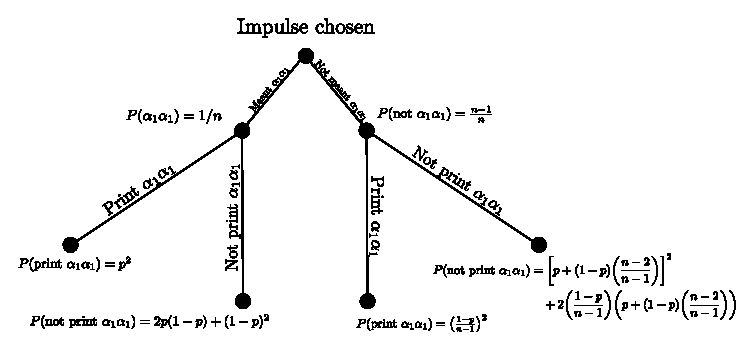
\includegraphics[width=\unitlength]{3.39.eps}}%
  \end{picture}%
  \end{center}
\endgroup%


\end{enumerate}

\newpage


% ============================================================================
% Chapter 4 - One-Dimensional Random Variables
% ============================================================================
% Restart the numbered theorem environments so each chapter numbers its own
% corollaries and propositions exactly as it did as a standalone document.
\setcounter{cor}{0}
\setcounter{prop}{0}
\setcounter{cor*}{0}

\phantomsection
\addcontentsline{toc}{section}{Solutions to Chapter 4: One-Dimensional Random Variables}
\section*{Solutions to Chapter 4: One-Dimensional Random Variables}

Unfinished problems: 4.23(a)(b), 4.26(a), 4.27(b)

\begin{enumerate}[label=4.\arabic*]
\itemsep0em 
%Question 4.1
\item  \begin{tcolorbox}[
  colback=Cerulean!5!white,
  colframe=Cerulean!75!black]
\textbf{A coin is known to come up heads three times as often as tails. This coin is tossed three times. Let $\bm{X}$ be the number of heads that appear. Write out the probability distribution of $\bm{X}$ and also the cdf. Make a sketch of both.}
\end{tcolorbox}

We have $X = \{0, 1, 2, 3 \}$. By premise, $P(H) = 3/4, P(T) = 1/4$. The sample space is 

\[ \{ HHH, HHT, HTH, THH, HTT, THT, TTH, TTT \} \] 

It follows that $P(X = 0) = 1/64, P(X = 1) = 9/64, P(X = 2) = 27/64, P(X = 3) = 27/64$. The corresponding cdf is $P(X \leq 0) = 1/64, P(X \leq 1) = 10/64, P(X \leq 2) = 37/64, P(X \leq 3) = 1$. Alternatively, since this is a binomial distribution, $P(X = 0) = \binom{3}{0}(3/4)^0 (1/4)^3 = 1/64, P(X = 1) = \binom{3}{1}(3/4)^1 (1/4)^2 = 9/64, P(X = 2) = \binom{3}{2}(3/4)^2 (1/4)^1 = 27/64, P(X = 3) = \binom{3}{3}(3/4)^3 (1/4)^0 = 27/64$. Graphically,

\begin{center}
\begin{tikzpicture}[scale=0.75]
	\begin{axis}
	[% 
	scatter/classes={%
		a={mark=square*,blue},%
		b={mark=triangle*,red},%
		c={mark=o,draw=black}},
		xlabel={$X$},
		ylabel={$P(X)$},
		xtick={0, 1, 2, 3},
		ytick={0.25, 0.5, 0.75, 1},
		ymax=1]
	\addplot[scatter,only marks,%
		scatter src=explicit symbolic]%
	table[meta=label] {
x     y      label
0      0.0156   a     
1      0.1406   a     
2      0.4219   a
3      0.4219   a     
	};
	\end{axis}
	\node[align=center,font=\bfseries, xshift=1.5em, yshift=1em] (title) 
    at (current bounding box.north)
    {Probability Distribution};
\end{tikzpicture}
\begin{tikzpicture}[scale=0.75]
	\begin{axis}
	[% 
	scatter/classes={%
		a={mark=square*,blue},%
		b={mark=triangle*,red},%
		c={mark=o,draw=black}},
		xlabel={$X$},
		ylabel={$P(X)$},
		xtick={0, 1, 2, 3},
		ytick={0.25, 0.5, 0.75, 1},
		ymax=1]
	\addplot[scatter,only marks,%
		scatter src=explicit symbolic]%
	table[meta=label] {
x     y      label
0      0.0156   a     
1      0.1562   a     
2      0.5781   a
3      1   a     
	};
	\end{axis}
		\node[align=center,font=\bfseries, xshift=1.5em, yshift=1em] (title) 
    at (current bounding box.north)
    {Cumulative Distribution Function};
\end{tikzpicture}
\end{center}

%Question 4.2
\item  \begin{tcolorbox}[
  colback=Cerulean!5!white,
  colframe=Cerulean!75!black]
\textbf{From a lot containing 25 items, 5 of which are defective, 4 are chosen at random. Let $\bm{X}$ be the number of defectives found. Obtain the probability distribution of $\bm{X}$ if}
\end{tcolorbox}

Let $X$ be the number of defectives found in a set of four. We have $\{ X = 0, 1, 2, 3, 4\}$. Then the sample space is (for $D = $ defective and $N =$ normal)
	
\begin{align*}
\{ NNNN, DNNN, NDNN, NNDN, NNND, DDNN, NDDN, NNDD, DNDN, \\
NDND, DNND, DDDN, NDDD, DDND, DNDD, DDDD \}
\end{align*}

	\begin{enumerate}
	%Question 4.2(a)
	\item  \begin{tcolorbox}[
	  colback=Cerulean!5!white,
	  colframe=Cerulean!75!black]
	\textbf{the items are chosen with replacement,}
	\end{tcolorbox}
	
	\begin{align*}
	P(X = 0) &= (4/5)^4 = 0.4096 \\
	P(X = 1) &=  4 \cdot (4/5)^3 (1/5) = 0.4096 \\
	P(X = 2) &= 6 \cdot (4/5)^2 (1/5)^2 = 0.1536 \\
	P(X = 3) &= 4 \cdot (4/5) (1/5)^3 = 0.0256 \\
	P(X = 4) &= (1/5)^4 = 0.0016
	\end{align*}
	
	Equivalently, since this is a binomial distribution, use $P(X = k) = \binom{4}{k} (1/5)^k (4/5)^{n-k}$ for $k = 0, ..., 4$.
	
	\begin{center}
\begin{tikzpicture}[scale=0.75]
	\begin{axis}
	[% 
	scatter/classes={%
		a={mark=square*,blue},%
		b={mark=triangle*,red},%
		c={mark=o,draw=black}},
		xlabel={$X$},
		ylabel={$P(X)$},
		xtick={0, 1, 2, 3, 4},
		ytick={0.25, 0.5, 0.75, 1},
		ymax=1]
	\addplot[scatter,only marks,%
		scatter src=explicit symbolic]%
	table[meta=label] {
x     y      label
0      0.4096   a     
1      0.4096   a     
2      0.1536   a
3      0.0256   a     
4	0.0016  a
	};
	\end{axis}
	\node[align=center,font=\bfseries, xshift=1.5em, yshift=1em] (title) 
    at (current bounding box.north)
    {Probability Distribution};
\end{tikzpicture}
\begin{tikzpicture}[scale=0.75]
	\begin{axis}
	[% 
	scatter/classes={%
		a={mark=square*,blue},%
		b={mark=triangle*,red},%
		c={mark=o,draw=black}},
		xlabel={$X$},
		ylabel={$P(X)$},
		xtick={0, 1, 2, 3, 4},
		ytick={0.25, 0.5, 0.75, 1},
		ymax=1]
	\addplot[scatter,only marks,%
		scatter src=explicit symbolic]%
	table[meta=label] {
x     y      label
0      0.4096   a     
1	0.8192  a
2      0.9728   a     
3      0.9984   a
4      1   a   	  
	};
	\end{axis}
		\node[align=center,font=\bfseries, xshift=1.5em, yshift=1em] (title) 
    at (current bounding box.north)
    {Cumulative Distribution Function};
\end{tikzpicture}
\end{center}
	
	%Question 4.2(b)
	\item  \begin{tcolorbox}[
	  colback=Cerulean!5!white,
	  colframe=Cerulean!75!black]
	\textbf{the items are chosen without replacement.}
	\end{tcolorbox}
	
	Critically, note that this is not a binomial distribution as each of the four successive drawings are \textbf{not} independent of one another. Then we calculate the probability of each outcome of $X$ as
	
	\begin{align*}
	P(X = 0) &= (20/25)(19/24)(18/23)(17/22) = 0.3830 \\
	P(X = 1) &= 4 \cdot (5/25)(20/24)(19/23)(18/22) = 0.4506 \\
	P(X = 2) &= 6 \cdot (5/25)(4/24)(20/23)(19/22) = 0.1502 \\
	P(X = 3) &= 4 \cdot (5/25)(4/24)(3/23)(20/22) = 0.0158 \\
	P(X = 4) &= (5/25)(4/24)(3/23)(2/22) = 0.0004
	\end{align*}
	
	Alternatively, observe that \textbf{with} replacement, the distribution is binomial, and \textbf{without}, it becomes hypergeometric. Then for any value of $X$, we can use the hypergeometric probability $\binom{5}{x} \binom{20}{4 - x} / \binom{25}{4}$.
	
		\begin{center}
\begin{tikzpicture}[scale=0.75]
	\begin{axis}
	[% 
	scatter/classes={%
		a={mark=square*,blue},%
		b={mark=triangle*,red},%
		c={mark=o,draw=black}},
		xlabel={$X$},
		ylabel={$P(X)$},
		xtick={0, 1, 2, 3, 4},
		ytick={0.25, 0.5, 0.75, 1},
		ymax=1]
	\addplot[scatter,only marks,%
		scatter src=explicit symbolic]%
	table[meta=label] {
x     y      label
0      0.3830   a     
1      0.4506   a     
2      0.1502   a
3      0.0158   a     
4	0.0004  a
	};
	\end{axis}
	\node[align=center,font=\bfseries, xshift=1.5em, yshift=1em] (title) 
    at (current bounding box.north)
    {Probability Distribution};
\end{tikzpicture}
\begin{tikzpicture}[scale=0.75]
	\begin{axis}
	[% 
	scatter/classes={%
		a={mark=square*,blue},%
		b={mark=triangle*,red},%
		c={mark=o,draw=black}},
		xlabel={$X$},
		ylabel={$P(X)$},
		xtick={0, 1, 2, 3, 4},
		ytick={0.25, 0.5, 0.75, 1},
		ymax=1]
	\addplot[scatter,only marks,%
		scatter src=explicit symbolic]%
	table[meta=label] {
x     y      label
0      0.3830   a     
1	0.8336  a
2      0.9838   a     
3      0.9996   a
4      1   a   	  
	};
	\end{axis}
		\node[align=center,font=\bfseries, xshift=1.5em, yshift=1em] (title) 
    at (current bounding box.north)
    {Cumulative Distribution Function};
\end{tikzpicture}
\end{center}
	\end{enumerate}

%Question 4.3
\item  \begin{tcolorbox}[
  colback=Cerulean!5!white,
  colframe=Cerulean!75!black]
\textbf{Suppose that the random variable $\bm{X}$ has possible values 1, 2, 3, ..., and $\bm{P(X = j) = 1/2^j, j = 1, 2, ...}$}
\end{tcolorbox}

	\begin{enumerate}
	%Question 4.3(a)
	\item  \begin{tcolorbox}[
	  colback=Cerulean!5!white,
	  colframe=Cerulean!75!black]
	\textbf{Compute $\bm{P(X \text{ is even})}$.}
	\end{tcolorbox}
	
	Observe that we derive the geometric series $P(X \text{ is even}) = \sum^\infty_{j = 2, 2 | j} 1/2^j = 1/4 + 1/16 + 1/64 + \cdots = \frac{1/4}{1 - 1/4} = \boxed{1/3}$.
	
	%Question 4.3(b)
	\item  \begin{tcolorbox}[
	  colback=Cerulean!5!white,
	  colframe=Cerulean!75!black]
	\textbf{Compute $\bm{P(X \geq 5)}$.}
	\end{tcolorbox}
	
	$\sum^\infty_{j = 1} 1/2^j - \sum^{4}_{j = 1} 1/2^j = \frac{1/2}{1 - 1/2} - (1/2 + 1/4 + 1/8 + 1/16) = \boxed{1/16}$.
	
	%Question 4.3(c)
	\item  \begin{tcolorbox}[
	  colback=Cerulean!5!white,
	  colframe=Cerulean!75!black]
	\textbf{Compute $\bm{P(X \text{ is divisible by }3)}$.}
	\end{tcolorbox}
	
	$\sum^\infty_{j = 3, 3 | j} 1/2^j = 1/8 + 1/64 + \cdots = \frac{1/8}{1 - 1/8} = \boxed{1/7}.$
	\end{enumerate}
	
%Question 4.4
\item  \begin{tcolorbox}[
  colback=Cerulean!5!white,
  colframe=Cerulean!75!black]
\textbf{Consider a random variable $\bm{X}$ with possible outcomes: 0, 1, 2, ... Suppose that $\bm{P(X = j) = (1 - a)a^j, j = 0, 1, 2, ...}$}
\end{tcolorbox}

	\begin{enumerate}
	%Question 4.4(a)
	\item  \begin{tcolorbox}[
	  colback=Cerulean!5!white,
	  colframe=Cerulean!75!black]
	\textbf{For what values of $\bm{a}$ is the above model meaningful?}
	\end{tcolorbox}
	
	By definition, a probability $p$ must be bounded by $0 \leq p \leq 1$, and this condition fails for $a < 0$ and $a > 1$. Therefore, we must have $0 \leq a \leq 1$. Really, we should be stricter and require $0 < a < 1$ as $P(X = j)$ vanishes otherwise.
	
	%Question 4.4(b)
	\item  \begin{tcolorbox}[
	  colback=Cerulean!5!white,
	  colframe=Cerulean!75!black]
	\textbf{Verify that the above does represent a legitimate probability distribution.}
	\end{tcolorbox}
	
	Satisfying Meyer Definition 1.3:
	
	\textbf{(1)} For $0 < a < 1$, $0 < (1 - a)a^j < 1 \ \forall j$. This is true for $j = 0$, as $0 < 1-a < 1$. Suppose it is true for $j = 1, ..., n-1$. Then it follows that $0 < (1 - a)a^n < (1-a)a^{n-1} < 1$. Therefore $0 < P(X = j) < 1$.
	
	\textbf{(2)} The sample space $S$ is choosing zero or any natural number. It follows that $P(S) = \sum^\infty_{j = 0} = (1 - a)a^j = (1-a) \frac{1}{1-a} = 1$.
	
	\textbf{(3)} For any arbitrary $j_i$ or $j_k$, $X = j_i$ and $X = j_k$ are mutually exclusive, for $X$ can only take on one value. Then $P(X = j_i \text{ or } X = j_k) = (1 - a)a^{j_i} + (1 - a)a^{j_k} = (1 - a)(a^{j_i} + a^{j_k})$.
	
	\textbf{(4)} See (2).
	
	%Question 4.4(c)
	\item  \begin{tcolorbox}[
	  colback=Cerulean!5!white,
	  colframe=Cerulean!75!black]
	\textbf{Show that for any two positive integers $\bm{s}$ and $\bm{t}$, $\bm{P(X > s + t | X > s) = P(X \geq t)}$.}
	\end{tcolorbox}
	
	\begin{proof}
	By definition of conditional probability:
	
	\begin{align*}
	P(X > s + t | X > s) &= \frac{P(X > s + t)}{P(X > s)} \\
	&= \frac{\sum^\infty_{j = s + t + 1} (1-a)a^j}{\sum^\infty_{j = s + 1} (1-a)a^j} \\
	&= \frac{\sum^\infty_{j = 0} (1-a)a^j - \sum^{s+t}_{j = 0} (1-a)a^j}{\sum^\infty_{j = 0} (1-a)a^j - \sum^{s}_{j = 0} (1-a)a^j} \\
	&= \frac{1 - (1 - a^{s+t+1} ) }{1 - ( 1 - a^{s+1} ) } \\
	&= \frac{a^{s+t+1} }{a^{s+1} } \\
	&= a^t \\
	&= 1 - \Bigg( \frac{1 - a^t}{1-a} \Bigg) (1-a) \\
	&= \sum^\infty_{j = t} (1-a)a^j = P(X \geq t)
	\end{align*}
	\end{proof}
	\end{enumerate}
	
%Question 4.5
\item  \begin{tcolorbox}[
  colback=Cerulean!5!white,
  colframe=Cerulean!75!black]
\textbf{Suppose that twice as many items are produced (per day) by machine 1 as by machine 2. However, about 4 percent of the items from machine 1 tend to be defective while machine 2 produces only about 2 percent defectives. Suppose that the daily output of the two machines is combined. A random sample of 10 is taken from the combined output. What is the probability that this sample contains 2 defectives?}
\end{tcolorbox}

By premise, $P(M1) = 2/3$ and $P(M2) = 1/3$. Moreover, $P(D | M1) = 0.04$ and $P(D | M2) = 0.02$. By the law of total probability, $P(D) = P(D | M1) P(M1) + P(D | M2) P(M2) = (0.04)(2/3) + (0.02)(1/3) = 1/30$. Suppose that $n$ items are collectively produced by the two machines. Let $k = n/30$ be the number of defective items. Then the probability of finding 2 defectives in a sample of 10 is $\boxed{ \binom{k}{2} \binom{n-k}{8} / \binom{n}{10} }$.

%Question 4.6
\item  \begin{tcolorbox}[
  colback=Cerulean!5!white,
  colframe=Cerulean!75!black]
\textbf{Rockets are launched until the first successful launching has taken place. If this does not occur within 5 attempts, the experiment is halted and the equipment inspected. Suppose that there is a constant probability of 0.8 of having a successful launching and that successive attempts are independent. Assume that the cost of the first launching is $\bm{K}$ dollars while subsequent launchings cost $\bm{K/3}$ dollars. Whenever a successful launching takes place, a certain amount of information is obtained which may be expressed as financial gain of, say $\bm{C}$ dollars. If $\bm{T}$ is the net cost of this experiment, find the probability distribution of $\bm{T}$.}
\end{tcolorbox}

By independence of each successive launch, if $X$ is the $i$-th launch that the rocket successfully launches, we have

\begin{align*}
P(X = 1) &= 0.8 \\
P(X = 2) &= (0.2)(0.8) = 0.16 \\
P(X = 3) &= (0.2)^2 (0.8) = 0.032 \\
P(X = 4) &= (0.2)^3 (0.8) = 0.0064 \\
P(X = 5) &= (0.2)^4 (0.8) = 0.00128
\end{align*}

Each of these correspond to the probability that $T$ takes on a certain value for net cost. Namely, $P(T = C - K) = 0.8, P(T = C - (K + K/3)) = 0.16, P(T = C - (K + 2K/3)) = 0.032, P(T = C - 2K) = 0.0064, P(T = C - (2K + K/3)) = 0.00128$. Graphically,

\begin{center}
\begin{tikzpicture}[scale=0.75]
	\begin{axis}
	[% 
	scatter/classes={%
		a={mark=square*,blue},%
		b={mark=triangle*,red},%
		c={mark=o,draw=black}},
		xlabel={$T$},
		ylabel={$P(T)$},
		xtick={0, 1, 2, 3, 4},
		xticklabels={$C-K$, $C - (K + K/3)$, $C - (K + 2K/3)$, $C - 2K$, $C - (2K + K/3)$},x tick label style={rotate=45,anchor=east}],
		ytick={0.25, 0.5, 0.75, 1},
		ymax=1]
	\addplot[scatter,only marks,%
		scatter src=explicit symbolic]%
	table[meta=label] {
x     y      label
0      0.8   a     
1	0.16  a
2      0.032   a     
3      0.0064   a
4      0.00128   a   	  
	};
	\end{axis}
		\node[align=center,font=\bfseries, xshift=1.5em, yshift=1em] (title) 
    at (current bounding box.north)
    {Probability Distribution of $T$};
\end{tikzpicture}
\end{center}

%Question 4.7
\item  \begin{tcolorbox}[
  colback=Cerulean!5!white,
  colframe=Cerulean!75!black]
\textbf{Evaluate $\bm{P(X = 5)}$, where $\bm{X}$ is the random variable defined in Example 4.10. Suppose that $\bm{n_1 = 10}$, $\bm{n_2 = 15}$, $\bm{p_1 = 0.3}$, and $\bm{p_2 = 0.2}$.}
\end{tcolorbox}

Example 4.10 describes a situation in which there is a machine that, in the first $n_1$ attempts at operating it, there is a constant probability $p_1$ of making no error, and then in the following $n_2$ operation attempts, there is a constant probability of $p_2$ of making no error. The objective is to find the total number of successful operations of the machine across the $n_1 + n_2 = n$ operations.

The set up is as follows: let $X = k$ be the number of correct operations. Let $Y_1 = r$ and $Y_2 = k - r$ be the correct operations accomplished in the $n_1$ and $n_2$ attempts, respectively. Observe that for any $k$ and $r$, and if $S_1, S_2$ are successful operations in the $n_1$ and $n_2$ attempts, the successive attempts will look like

\[ \underbrace{ \underbrace{S_1 S_1 \cdots S_1}_{r} \underbrace{ \bar{S_1} \bar{S_1} \cdots \bar{S_1} }_{n_1 - r} }_{n_1} \underbrace{ \underbrace{S_2 S_2 \cdots S_2}_{k-r} \underbrace{ \bar{S_2} \bar{S_2} \cdots \bar{S_2} }_{n_2 - (k - r)} }_{n_2} \]

For some fixed $r,k$, we can see that there are $\binom{n_1}{r}$ ways of $r$ successes appearing out of $n_1$ attempts, and correspondingly, $\binom{n_2}{k-r}$ ways of $k-r$ success out of $n_2$ attempts. The probability $P(Y_1 = r)$ is then $\binom{n_1}{r} p_1^r (1-p_1)^{n_1 - r}$, and $P(Y_2 = k-r)$ is $\binom{n_2}{k - r} p_2^{k-r} (1 - p_2)^{n_2 - (k - r)}$; note that \textit{within} each of the $n_1, n_2$ attempts the probabilities of success or failure are constant and independent, which allows us to derive these equations. Now, because $Y_1$ and $Y_2$ are \textit{themselves} independent, to find the probability of $r$ successful operations in $n_1$ attempts \textit{and} $k-r$ successful operations in $n_2$ attempts is equivalent to writing

\[ P(X = k, Y_1 = r, Y_2 = k - r)=  \binom{n_1}{r} p_1^r (1-p_1)^{n_1 - r} \binom{n_2}{k - r} p_2^{k-r} (1 - p_2)^{n_2 - (k - r)} \]

However, the desired probability is to find $P(X = k)$. Applying the law of total probability for \textit{all} values of $r$ (since the events $Y_1 = r_1, Y_1 = r_2, ...$ are mutually exclusive) gives us

\[ P(X = k) = \sum^{n_1}_{r = 0} \binom{n_1}{r} p_1^r (1-p_1)^{n_1 - r} \binom{n_2}{k - r} p_2^{k-r} (1 - p_2)^{n_2 - (k - r)}  \] 

For the given values $k = 5, n_1 = 10, n_2 = 15, p_1 = 0.3, p_2 = 0.2$, we calculate

\[ P(X = 5) = \sum^{10}_{r = 0} \binom{10}{r} (0.3)^r (0.7)^{10 - r} \binom{15}{5 - r} (0.2)^{5-r} (0.8)^{(20 + r)} = \boxed{0.0189} \]

%Question 4.8
\item  \begin{tcolorbox}[
  colback=Cerulean!5!white,
  colframe=Cerulean!75!black]
\textbf{(\textit{Properties of the binomial probabilities.}) In the discussion of Example 4.8 a general pattern for the binomial probabilities $\binom{n}{k} \bm{p^k (1-p)^{n-k}}$ was suggested. Let us denote these probabilities by $\bm{p_n (k)}$.}
\end{tcolorbox}

	\begin{enumerate}
	%Question 4.8(a)
	\item  \begin{tcolorbox}[
	  colback=Cerulean!5!white,
	  colframe=Cerulean!75!black]
	\textbf{Show that for $\bm{0 \leq k < n}$ we have $\bm{p_n (k+1) / p_n (k) = [(n-k) / (k+1)] [p / (1 - p)]}$}
	\end{tcolorbox}
	
	\begin{proof}
	We have $p_n (k + 1) = \binom{n}{k+1} p^{k+1} (1-p)^{n-(k+1)} = \frac{n!}{(k+1)! (n- (k+1))!} p^{k+1} (1-p)^{n-(k+1)}$ and $p_n (k) = \binom{n}{k} p^k (1-p)^{n-k} = \frac{n!}{k! (n-k)!}  p^k (1-p)^{n-k}$. It immediately follows that $p_n (k+1) / p_n (k) = [(n-k) / (k+1)] [p / (1 - p)]$.
	\end{proof}
	
	%Question 4.8(b)
	\item  \begin{tcolorbox}[
	  colback=Cerulean!5!white,
	  colframe=Cerulean!75!black]
	\textbf{Using (a) show that}
	\end{tcolorbox}
	
		\begin{enumerate}
		%Question 4.8(b)(i)
		\item  \begin{tcolorbox}[
	  	colback=Cerulean!5!white,
	  	colframe=Cerulean!75!black]
		\textbf{$\bm{p_n (k + 1) > p_n (k)}$ if $\bm{k < np - (1 - p)}$,}
		\end{tcolorbox}
		
		\begin{proof}
		Equivalently, we demonstrate that $p_n (k+1) / p_n (k) > 1$. Suppose $k < np - (1 - p)$. Then $n - k > n - np + (1-p) = (1 - p)(n + 1)$ and $k + 1 < np - (1 - p) + 1 = p(n+1)$. Then $\frac{n-k}{k+1} > \frac{(1-p)(n+1)}{p(n+1)} = \frac{1-p}{p}$, implying $p_n (k+1) / p_n (k) = \frac{n-k}{k+1} \frac{p}{1-p} > \frac{1-p}{p} \frac{p}{1-p} = 1$.
		\end{proof}
		
		%Question 4.8(b)(ii)
		\item  \begin{tcolorbox}[
	  	colback=Cerulean!5!white,
	  	colframe=Cerulean!75!black]
		\textbf{$\bm{p_n (k + 1) = p_n (k)}$ if $\bm{k = np - (1 - p)}$,}
		\end{tcolorbox}
		
		\begin{proof}
		Equivalently, we demonstrate that $p_n (k+1) / p_n (k) = 1$. Suppose $k = np - (1 - p)$. Then $n - k = n - np + (1-p) = (1 - p)(n + 1)$ and $k + 1 = np - (1 - p) + 1 = p(n+1)$. Then $\frac{n-k}{k+1} = \frac{(1-p)(n+1)}{p(n+1)} = \frac{1-p}{p}$, implying $p_n (k+1) / p_n (k) = \frac{n-k}{k+1} \frac{p}{1-p} = \frac{1-p}{p} \frac{p}{1-p} = 1$.
		\end{proof}
		
			%Question 4.8(b)(iii)
		\item  \begin{tcolorbox}[
	  	colback=Cerulean!5!white,
	  	colframe=Cerulean!75!black]
		\textbf{$\bm{p_n (k + 1) < p_n (k)}$ if $\bm{k > np - (1 - p)}$.}
		\end{tcolorbox}
		
		\begin{proof}
		Equivalently, we demonstrate that $p_n (k+1) / p_n (k) < 1$. Suppose $k > np - (1 - p)$. Then $n - k < n - np + (1-p) = (1 - p)(n + 1)$ and $k + 1 > np - (1 - p) + 1 = p(n+1)$. Then $\frac{n-k}{k+1} < \frac{(1-p)(n+1)}{p(n+1)} = \frac{1-p}{p}$, implying $p_n (k+1) / p_n (k) = \frac{n-k}{k+1} \frac{p}{1-p} < \frac{1-p}{p} \frac{p}{1-p} = 1$.
		\end{proof}
		\end{enumerate}
		
	%Question 4.8(c)
	\item  \begin{tcolorbox}[
	  colback=Cerulean!5!white,
	  colframe=Cerulean!75!black]
	\textbf{Show that if $\bm{np - (1 - p)}$ is an integer, $\bm{p_n (k)}$ assumes its maximum value for two values of $\bm{k}$, namely $\bm{k_0 = np - (1 - p)}$ and $\bm{k'_0 = np - (1 - p) + 1}$.}
	\end{tcolorbox}
	
	\begin{proof}
	By (b)(ii), if $k_0 = np - (1-p)$, then $p_n (k_0) = p_n (k_0 + 1) = p_n (k'_0)$, the last equality from the fact that $k_0 + 1 = k'_0 = np - (1-p) + 1$. By (b)(i), $k_0 - 1 < k_0 \implies p_n(k_0) > p_n(k_0 - 1)$; ``induce downwards" to ascertain that decreasing $k_0 - 1, k_0 - 2,...$ implies that $p_n (k_0 - 1) > p_n (k_0 - 2) > \cdots$. Analogously, by (b)(iii), $k'_0 > k_0 \implies p_n(k'_0 + 1) < p_n(k'_0)$; ``induce upwards" to likewise ascertain that increasing $k'_0 + 1, k'_0 + 2, ...$ implies $p_n (k'_0 + 1) > p_n(k'_0 + 2) > \cdots$. Therefore, since values of $k$ moving away from $k_0, k'_0$ on either side cause $p_n$ to monotonically decrease, it follows that $k_0, k'_0$ are the maxima for $p_n$. \\
	
	Intuitively, this tells us that if $k_0 = np - (1-p)$ is an integer, then the binomial distribution will have \textit{two} modes differing by one.
	\end{proof}
	
	%Question 4.8(d)
	\item  \begin{tcolorbox}[
	  colback=Cerulean!5!white,
	  colframe=Cerulean!75!black]
	\textbf{Show that if $\bm{np - (1 - p)}$ is not an integer, $\bm{p_n (k)}$ assumes its maximum value when $\bm{k}$ is equal to the smallest integer greater than $\bm{k_0}$.}
	\end{tcolorbox}
	
	\begin{proof}\textbf{Strategy:} Define the \textbf{ceiling} $\lceil a \rceil$ of a real number $a$ as the smallest integer greater than $a$. If $k_0 = np - (1-p) \notin \mathbb{Z}$, then define $\lceil k_0 \rceil - k_0 = r$, for some $r, 0 < r < 1$; therefore, $\lceil k_0 \rceil = np - (1-p) + r$. The task before us is to evaluate if $p_n (\lceil k_o \rceil) > p_n (\lceil k_o \rceil - 1)$ and $p_n (\lceil k_o \rceil) > p_n (\lceil k_o \rceil + 1)$, or equivalently, if $\frac{p_n (\lceil k_o \rceil)}{p_n (\lceil k_o \rceil - 1)} > 1$ and $\frac{p_n (\lceil k_o \rceil + 1)}{p_n (\lceil k_o \rceil) } < 1$. Should we ascertain these conditions, then we may apply the monotonicity results of part (b) and conclude that $k = \lceil k_o \rceil$ is the (singular) maximum of of $p_n(k)$.
	
	First we consider the left-flank of $\lceil k_o \rceil$:
	
	\begin{align*}
	\frac{p_n (\lceil k_o \rceil)}{p_n (\lceil k_o \rceil - 1)} &= \frac{n - \lceil k_0 \rceil + 1}{\lceil k_0 \rceil} \frac{p}{1-p} \\
	&= \frac{n - ( np - (1-p) + r ) + 1}{np - (1-p) + r} \frac{p}{1-p} \\
	&= \frac{(1-p)(n+1) + (1-r)}{p(n+1) - (1-r)} \frac{p}{1-p} \\
	&> \frac{(1-p)(n+1)}{p(n+1)} \frac{p}{1-p} = 1
	\end{align*}
	
	And now the right-flank:
	
	\begin{align*}
	\frac{p_n (\lceil k_o \rceil + 1)}{p_n (\lceil k_o \rceil)} &= \frac{n - \lceil k_0 \rceil}{\lceil k_0 \rceil - 1} \frac{p}{1-p} \\
	&= \frac{n - (np - (1-p) + r)}{np - (1-p) + r + 1} \frac{p}{1-p} \\
	&= \frac{n (1-p) + (1-p) - r}{p(n+1) + r} \frac{p}{1-p} \\
	&< \frac{(1-p)(n+1)}{p(n+1)} \frac{p}{1-p} = 1
	\end{align*}
	
	In general, it can be shown that for any integer $i$, $0 \leq i \leq \lceil k_0 \rceil$, it is true that $\frac{p_n (\lceil k_o \rceil - i)}{p_n (\lceil k_o \rceil - (i+1))} > 1$, and analogously, $\frac{p_n (\lceil k_o \rceil + (j + 1))}{p_n (\lceil k_o \rceil + j)} < 1$ for any integer $j$, $0 \leq j \leq n - \lceil k_0 \rceil - 1$. Therefore, $p_n (\lceil k_0 \rceil)$ is the singular maximum.
	
	\end{proof}
	
	%Question 4.8(e)
	\item  \begin{tcolorbox}[
	  colback=Cerulean!5!white,
	  colframe=Cerulean!75!black]
	\textbf{Show that if $\bm{np - (1 - p) < 0}$, $\bm{p_n(0) > p_n(1) > \cdots > p_n(n)}$ while if $\bm{np - (1-p) = 0, p_n(0) = p_n(1) > p_n(2) > \cdots > p_n(n)}$.}
	\end{tcolorbox}
	
	\begin{proof}
	In the first case, apply (b)(iii) and since $k \geq 0 > np - (1-p)$, for $k = 0$ we have $p_n(0) > p_n(1)$, for $k=1$, $p_n(1) > p_n(2)$, and so-on-and-so-forth until $k = n-1$, $p_n (n-1) > p_n(n)$, establishing the result. In the second case, apply (b)(ii) for $k = np - (1-p) = 0$, therefore $p_n (0) = p_n(1)$, and for $k > np - (1-p) = 0$, apply (b)(iii) to get the desired result.
	\end{proof}

	\end{enumerate}

%Question 4.9
\item  \begin{tcolorbox}[
  colback=Cerulean!5!white,
  colframe=Cerulean!75!black]
\textbf{The continuous random variable $\bm{X}$ has pdf $\bm{f(x) = x/2, 0 \leq x \leq 2}$. Two independent determinations of $\bm{X}$ are made. What is the probability that both these determinations will be greater than one? If three independent determinations had been made, what is the probability that exactly two of these are larger than one?}
\end{tcolorbox}

In one determination, $P(1 < X) = \int^2_1 \frac{x}{2}dx = \frac{x^2}{4} \Big|^2_1 = 3/4$. By premise, each determination is independent, so we need only calculate $P(1 < X) P(1 < X) = \boxed{9/16}$. For the second case, there are $\binom{3}{2}$ ways in which exactly two of the three determinations are larger than one. The probability of one such scenario is $P(1 < X) P(1 < X) P(X \leq 1) = (3/4)^2 \cdot \int^1_0 \frac{x}{2}dx = (3/4)^2 1/4 = 9/64$. Multiply by $\binom{3}{2} = 3$ to get $\boxed{27/64}$. 

%Question 4.10
\item  \begin{tcolorbox}[
  colback=Cerulean!5!white,
  colframe=Cerulean!75!black]
\textbf{Let $\bm{X}$ be the life length of an electron tube and suppose that $\bm{X}$ may be represented as a continuous random variable with pdf $\bm{f(x) = be^{-bx}}$, $\bm{x \geq 0}$. Let $\bm{p_j} = P(j \leq X < j + 1)$. Show that $\bm{p_j}$ is of the form $\bm{(1-a)a^j}$ and determine $\bm{a}$.}
\end{tcolorbox}

Given the probability distribution function, we derive

\begin{align*}
\int^{j+1}_{j} be^{-bx} dx &= -e^{-bx} \Big|^{j+1}_j \\
&= -e^{-(j+1)x} + e^{-jx} \\
&= e^{-jx} (1 - e^{-x} ) \\
\end{align*}

Let $a = e^{-x}$, then the above becomes $(1-a)a^j$.

%Question 4.11
\item  \begin{tcolorbox}[
  colback=Cerulean!5!white,
  colframe=Cerulean!75!black]
\textbf{The continuous random variable $\bm{X}$ has pdf $\bm{f(x) = 3x^2, -1 \leq x \leq 0}$. If $\bm{b}$ is a number satisfying $\bm{-1 < b < 0}$, compute $\bm{P(X > b | X < b/2)}$.}
\end{tcolorbox}

By definition of conditional probability,

\begin{align*}
P(X > b | X < b/2) &= \frac{P(b < X < b/2)}{P(X < b/2)} \\
&= \frac{\int^{b/2}_b 3x^2 dx}{\int^{b/2}_{-1} 3x^2 dx} \\
&= \frac{x^3 \Big|^{b/2}_b}{x^3 \Big|^{b/2}_{-1}} \\
&= \frac{b^3/8 - b^3}{b^3/8 + 1} \\
&= \boxed{ \frac{-7b^3}{b^3 + 8} }
\end{align*}

%Question 4.12
\item  \begin{tcolorbox}[
  colback=Cerulean!5!white,
  colframe=Cerulean!75!black]
\textbf{Suppose that $\bm{f}$ and $\bm{g}$ are pdf's on the same interval, say $\bm{a \leq x \leq b}$.}
\end{tcolorbox}

	\begin{enumerate}
	%Question 4.12(a)
	\item  \begin{tcolorbox}[
	  colback=Cerulean!5!white,
	  colframe=Cerulean!75!black]
	\textbf{Show that $\bm{f + g}$ is not a pdf on that interval.}
	\end{tcolorbox}
	
	(Note: $\int$ shall mean $\int^{+\infty}_{-\infty}$)
	
	\begin{proof}
	By premise, $\int f(x) dx = 1$ and $\int g(x) dx = 1$. Then $\int f(x) dx + \int g(x) dx = \int (f(x) + g(x))dx = 2$, contradicting the definition of a probability distribution function. 
	\end{proof}
	
	%Question 4.12(b)
	\item  \begin{tcolorbox}[
	  colback=Cerulean!5!white,
	  colframe=Cerulean!75!black]
	\textbf{Show that for every number $\bm{\beta}$, $\bm{0 < \beta < 1, \beta f(x) + (1- \beta)g(x)}$ is a pdf on that interval.}
	\end{tcolorbox}
	
	\begin{proof}
	(1) By premise, $f(x), g(x) \geq 0$. Then $\beta f(x), (1 - \beta)g(x) \geq 0$ since $0 < \beta < 1$. \\
	(2) \begin{align*}
	\int ( \beta f(x) + (1- \beta)g(x) ) dx &= \int \beta f(x) dx + \int (1 - \beta) g(x) dx \\
	&= \beta \int f(x) dx + (1 - \beta) \int g(x) dx \\
	&= \beta + 1 - \beta = 1
	\end{align*}
	(3) By premise, $\int^b_a f(x) dx$ and $\int^b_a g(x) dx$ exist. For any $(a,b), a, b \in (-\infty, + \infty)$, it follows that
	\begin{align*}
	\beta \int^b_a  f(x) dx + (1 - \beta) \int^b_a  g(x) dx &= \int^b_a \beta f(x) dx + \int^b_a (1-\beta) g(x) dx \\
	&= \int^b_a ( \beta f(x) + (1- \beta)g(x) ) dx
	\end{align*}
	\end{proof}
	
	\end{enumerate}

%Question 4.13
\item  \begin{tcolorbox}[
  colback=Cerulean!5!white,
  colframe=Cerulean!75!black]
\textbf{Suppose that the graph in Fig. 4.16 represents the pdf of a random variable $\bm{X}$.}
\end{tcolorbox}

\begin{center}
	\begin{tikzpicture}[scale=0.75]
	\begin{axis}[
    	axis lines = center,
		ymax=7,
		ymin=0,
		xmin=-10,
		xmax=10,
   		 xlabel = \( x \),
   		 ylabel = {\( f(x) \)},
		 xtick={-8,0,6},
    		 xticklabels={$x=-a$,$$,$x=b$},
		 ytick={},
		 yticklabels={},
		]
	\addplot[domain=-8:4, style=very thick, color=red]{0.5*x+4};
	\addplot[domain=4:6, style=very thick, color=red]{-3*x+18};
	\node[draw] at (150,650) {$(a,b)$};
	\end{axis}
	\end{tikzpicture}
	\end{center}

	\begin{enumerate}
	%Question 4.13(a)
	\item  \begin{tcolorbox}[
	  colback=Cerulean!5!white,
	  colframe=Cerulean!75!black]
	\textbf{What is the relationship between $\bm{a}$ and $\bm{b}$?}
	\end{tcolorbox}
	
	The pdf is defined as
	
	\[f(x) = \begin{cases}
  \frac{b}{2a}x + \frac{b}{2},  &  -a \leq x < a \\
  \frac{b}{a-b} x - \frac{b^2}{a - b}, & a \leq x \leq b
\end{cases} \]

	Then it must be shown that the relationship between $a$ and $b$ is such that 
	
	\[ \int^a_{-a} \bigg( \frac{b}{2a} x + \frac{b}{2} \bigg) dx + \int^b_a \bigg( \bigg( \frac{b}{a-b} \bigg) x - \frac{b}{a-b} \bigg) dx = 1 \]
	
	With some algebra, it follows that $\boxed{a = (2/b) - b}$.
	
	%Question 4.13(b)
	\item  \begin{tcolorbox}[
	  colback=Cerulean!5!white,
	  colframe=Cerulean!75!black]
	\textbf{If $\bm{a > 0}$ and $\bm{b > 0}$, what can you say about the largest value which $\bm{b}$ may assume?}
	\end{tcolorbox}
	
	Fixing these constraints, we must have $0 < (2/b) - b \implies b^2 < 2 \implies \boxed{b < \sqrt{2}}$.
	\end{enumerate}
	
%Question 4.14
\item  \begin{tcolorbox}[
  colback=Cerulean!5!white,
  colframe=Cerulean!75!black]
\textbf{The percentage of alcohol $\bm{(100X)}$ in a certain compound may be considered as a random variable, where $\bm{X, 0 < X < 1}$, has the following pdf: $\bm{f(x) = 20 x^3 (1-x), 0 < x < 1}$}
\end{tcolorbox}

	\begin{enumerate}
	%Question 4.14(a)
	\item  \begin{tcolorbox}[
	  colback=Cerulean!5!white,
	  colframe=Cerulean!75!black]
	\textbf{Obtain an expression for the cdf $\bm{F}$ and sketch its graph.}
	\end{tcolorbox}
	
	By definition of cumulative distribution function, $F(x) = \int^x_0 20x^3 (1-x)dx = \boxed{5x^4 - 4x^5}$.
	
	\begin{center}
	\begin{tikzpicture}[scale=0.75]
	\begin{axis}[
    		axis lines = left,
		ymax=1,
		ymin=0,
   		 xlabel = \( X \),
   		 ylabel = {\( F(x) \)},
		 xtick={0,1},
    		 xticklabels={$0$,$1$},
		 ytick={0,1,1.5},
		 yticklabels={$0$,$1$,$$},
		]
	\addplot[domain=0:1, style=very thick, color=red]{5*x^4 - 4*x^5};
	\addplot[domain=1:1.5, style=very thick, color=red]{1};
	\end{axis}
	\end{tikzpicture}
	\end{center}
	
	%Question 4.14(b)
	\item  \begin{tcolorbox}[
	  colback=Cerulean!5!white,
	  colframe=Cerulean!75!black]
	\textbf{Evaluate $\bm{P(X \leq 2/3)}$.}
	\end{tcolorbox}
	
	$P(X \leq 2/3) = \int^{2/3}_0 = 20x^3 (1-x)dx = 5x^4 - 4x^5 \Big|^{2/3}_0 = \boxed{0.461}$
	
	%Question 4.14(c)
	\item  \begin{tcolorbox}[
	  colback=Cerulean!5!white,
	  colframe=Cerulean!75!black]
	\textbf{Suppose that the selling price of the above compound depends on the alcohol content. Specifically, if $\bm{1/3 < X < 2/3}$, the compound sells for $\bm{C_1}$ dollars/gallon; otherwise it sells for $\bm{C_2}$ dollars/gallon. If the cost is $\bm{C_3}$ dollars/gallon, find the probability distribution of the net profit per gallon.}
	\end{tcolorbox}
	
	$P(1/3 < X < 2/3) = \int^{2/3}_{1/3} 20x^3 (1-x)dx = 5x^4 - 4x^4 \Big|^{2/3}_{1/3} = \boxed{0.416}$
	
	Therefore, $P(\text{net profit is } C_1 - C_3) = \boxed{0.416}$ and $P(\text{net profit is } C_2 - C_3) = \boxed{0.584}$.
	\end{enumerate}

%Question 4.15
\item  \begin{tcolorbox}[
  colback=Cerulean!5!white,
  colframe=Cerulean!75!black]
\textbf{Let $\bm{X}$ be a continuous random variable with pdf $\bm{f}$ given by:}
\end{tcolorbox}

\[ f(x) = \begin{cases}
  ax  & 0 \leq x \leq 1 \\
  a & 1 \leq x \leq 2 \\
  -ax + 3a & 2 \leq x \leq 3 \\
  0 & \text{elsewhere}
\end{cases} \]

	\begin{enumerate}
	%Question 4.15(a)
	\item  \begin{tcolorbox}[
	  colback=Cerulean!5!white,
	  colframe=Cerulean!75!black]
	\textbf{Determine the constant $\bm{a}$.}
	\end{tcolorbox}
	
	By the Kolmogorov probability axioms, the definite integral of a pdf across the reals must be unity. Therefore, we must find a value of $a$ that acquiesces to this condition. We calculate:
	
	\begin{align*}
	&\int^1_0 ax dx + \int^2_1 adx + \int^3_2 (-ax + 3a)dx = 1 \\
	&\implies \frac{ax^2}{2} \Big|^1_0 + ax \Big|^2_1 + \Big( -\frac{ax^2}{2} + 3ax \Big) \Big|^3_2 = 1 \\
	&\implies \boxed{a = 1/2}
	\end{align*}
	
	%Question 4.15(b)
	\item  \begin{tcolorbox}[
	  colback=Cerulean!5!white,
	  colframe=Cerulean!75!black]
	\textbf{Determine $\bm{F}$, the cdf, and sketch its graph.}
	\end{tcolorbox}
	
	The cdf is defined as follows:
	
	$0 \leq X \leq 1: \int^x_0 \frac{1}{2}x dx = \frac{x^2}{4}$
	
	$1 \leq X \leq 2: \int^1_0 \frac{1}{2}x dx + \int^x_1 \frac{1}{2} dx = \frac{1}{4} + \frac{1}{2}x - \frac{1}{2}$
	
	$2 \leq X \leq 3: \int^1_0 \frac{1}{2}x dx + \int^2_1 \frac{1}{2} dx + \int^x_2 (-\frac{1}{2} x + \frac{3}{2} ) dx = \frac{1}{4} + 1 - \frac{1}{2} + ( -\frac{x^2}{4} + \frac{3}{2}x ) - 2$
	
	Therefore,
	
	\[ F(x) = \begin{cases}
  \frac{x^2}{4}  & 0 \leq X \leq 1 \\
  \frac{1}{2}x - \frac{1}{4} & 1 \leq X \leq 2 \\
  -\frac{x^2}{4} + \frac{3}{2}x - \frac{5}{4} & 2 \leq X \leq 3 \\
  1 & X \geq 3
\end{cases} \]

	\begin{center}
	\begin{tikzpicture}[scale=0.75]
	\begin{axis}[
    		axis lines = left,
		ymax=1,
		ymin=0,
   		 xlabel = \( X \),
   		 ylabel = {\( F(x) \)},
		 xtick={0,1,2,3},
    		 xticklabels={$0$,$1$,$2$,$3$},
		 ytick={0,1},
		 yticklabels={$0$,$1$},
		]
	\addplot[domain=0:1, color=red, style=very thick]{1/4*x^2};
	\addplot[domain=1:2, color=red, style=very thick]{1/2*x - 1/4};
	\addplot[domain=2:3, color=red, style=very thick]{-1/4*x^2 + 3/2*x - 5/4};
	\addplot[domain=3:3.5, color=red, style=very thick]{1};
	\end{axis}
	\end{tikzpicture}
	\end{center}
	
	%Question 4.15(c)
	\item  \begin{tcolorbox}[
	  colback=Cerulean!5!white,
	  colframe=Cerulean!75!black]
	\textbf{If $\bm{X_1, X_2,}$ and $\bm{X_3}$ are three independent observations from $\bm{X}$, what is the probability that exactly one of these three numbers is larger than 1.5?}
	\end{tcolorbox}
	
	Equivalently, one of the three independent observations is greater than 1.5 and the other two less than or equal to 1.5. There are $\binom{3}{1}$ such configurations. For any $X_i, P(X_i \leq 1.5) = (1/2)(3/2) - 1/4 = 1/2$. By complementary events, $P(X_i > 1.5) = 1/2$. Then we calculate $\binom{3}{1} (1/2)^3 = \boxed{3/8}$.
	\end{enumerate}
	
%Question 4.16
\item  \begin{tcolorbox}[
  colback=Cerulean!5!white,
  colframe=Cerulean!75!black]
\textbf{The diameter on an electric cable, say $\bm{X}$, is assumed to be a continuous random variable with pdf $\bm{f(x) = 6x(1-x), 0 \leq x \leq 1}$.}
\end{tcolorbox}

	\begin{enumerate}
	%Question 4.16(a)
	\item  \begin{tcolorbox}[
	  colback=Cerulean!5!white,
	  colframe=Cerulean!75!black]
	\textbf{Check that the above is a pdf and sketch it.}
	\end{tcolorbox}
	
	(1) For $0 \leq x \leq 1$, $x^2 \leq x$, so it follows that $6x - 6x^2 = 6x(1-x) \geq 0$ \\
	(2) $\int^1_0 6x(1-x) = 3x^2 - 2x^3 \Big|^1_0 = 1$ \\
	(3) $P(a \leq X \leq b) = \int^b_a 6x(1-x)dx$
	
	Therefore, $f(x)$ is a pdf.
	
	\begin{center}
	\begin{tikzpicture}[scale=0.75]
	\begin{axis}[
    		axis lines = left,
		ymax=1.5,
		ymin=0,
   		 xlabel = \( x \),
   		 ylabel = {\( f(x) \)},
		 xtick={0,1},
    		 xticklabels={$0$,$1$},
		 ytick={0,1},
		 yticklabels={$0$,$1$},
		]
	\addplot[domain=0:1, samples = 500, color=red, style=very thick]{6*x*(1-x)};
	\end{axis}
	\end{tikzpicture}
	\end{center}
	
	%Question 4.16(b)
	\item  \begin{tcolorbox}[
	  colback=Cerulean!5!white,
	  colframe=Cerulean!75!black]
	\textbf{Obtain an expression for the cdf of $\bm{X}$ and sketch it.}
	\end{tcolorbox}
	
	$F(x) = \int^x_0 6x(1-x)dx = \boxed{3x^2 - 2x^3}$
	
	\begin{center}
	\begin{tikzpicture}[scale=0.75]
	\begin{axis}[
    		axis lines = left,
		ymax=1,
		ymin=0,
   		 xlabel = \( x \),
   		 ylabel = {\( f(x) \)},
		 xtick={0,1},
    		 xticklabels={$0$,$1$},
		 ytick={0,1},
		 yticklabels={$0$,$1$},
		]
	\addplot[domain=0:1, samples = 500, color=red, style=very thick]{3*x^2 - 2*x^3};
	\end{axis}
	\end{tikzpicture}
	\end{center}
	
	%Question 4.16(c)
	\item  \begin{tcolorbox}[
	  colback=Cerulean!5!white,
	  colframe=Cerulean!75!black]
	\textbf{Determine a number $\bm{b}$ such that $\bm{P(X < b) = 2P(X > b)}$.}
	\end{tcolorbox}
	
	\begin{align*}
	&\int^b_0 6x(1-x)dx = 2 \int^1_b 6x(1-x)dx \\
	&\implies 3b^2 - 2b^3 = 2(1 - 3b^2 + 2b^3) \\
	&\implies -6b^3 + 9b^2 - 2 = 0 \\
	&\implies \boxed{b = 0.613}
	\end{align*}
	
	Note that there are two positive roots, but because our pdf is defined over $0 \leq X \leq 1$, we choose the one root within that domain.
	
	%Question 4.16(d)
	\item  \begin{tcolorbox}[
	  colback=Cerulean!5!white,
	  colframe=Cerulean!75!black]
	\textbf{Compute $\bm{P(X \leq 1/2 | 1/3 < X < 2/3)}$.}
	\end{tcolorbox}
	
	\begin{align*}
	P(X \leq 1/2 | 1/3 < X < 2/3) &= \frac{P(1/3 < X < 1/2)}{P(1/3 < X < 2/3)} \\
	&= \frac{\int^{1/2}_{1/3} 6x(1-x)dx}{\int^{2/3}_{1/3} 6x(1-x)dx} \\
	&= \boxed{0.5}
	\end{align*}
	
	\end{enumerate}

%Question 4.17
\item  \begin{tcolorbox}[
  colback=Cerulean!5!white,
  colframe=Cerulean!75!black]
\textbf{Each of the following functions represents the cdf of a continuous random variable. In each case $\bm{F(x) = 0}$ for $\bm{x < a}$ and $\bm{F(x) = 1}$ for $\bm{x > b}$, where $\bm{[a,b]}$ is the indicated interval. In each case, sketch the function $\bm{F}$, determine the pdf $\bm{f}$ and sketch it. Also verify that $\bm{f}$ is a pdf.}
\end{tcolorbox}

	\begin{enumerate}
	%Question 4.17(a)
	\item  \begin{tcolorbox}[
	  colback=Cerulean!5!white,
	  colframe=Cerulean!75!black]
	\textbf{$\bm{F(x) = x/5, 0 \leq x \leq 5}$}
	\end{tcolorbox}
	
	By Theorem 4.4, $\frac{d}{dx} F(x) = 1/5 = f(x)$. Clearly, $1/5 \geq 0 \ \forall x \in [0,5]$. Additionally, $\int^5_0 1/5 dx = x/5 \Big|^5_0 = 1$, and $\forall a, b$ such that $ [a, b] \subseteq [0, 5]$, we have $P(a \leq X \leq b) = \int^b_a 1/5 dx$. Therefore, $f(x) = 1/5$ is a pdf.
	
	\begin{center}
	\begin{tikzpicture}[scale=0.75]
	\begin{axis}[
    		axis lines = left,
   		 xlabel = \( x \),
   		 ylabel = {\( f(x) \)},
		 xtick={0,5},
    		 xticklabels={$0$,$5$},
		 ytick={0,1},
		 yticklabels={$0$,$1$},
		]
	\addplot[domain=0:5, samples = 500, color=red, style=very thick]{1/5};
	\end{axis}
	\end{tikzpicture}
	\end{center}
	
	%Question 4.17(b)
	\item  \begin{tcolorbox}[
	  colback=Cerulean!5!white,
	  colframe=Cerulean!75!black]
	\textbf{$\bm{F(x) = (2/ \pi) \arcsin (\sqrt{x}), 0 \leq x \leq 1}$}
	\end{tcolorbox}
	
	By Theorem 4.4, $\frac{d}{dx} F(x) = \frac{2}{\pi} \frac{1}{\sqrt{1-x}} \frac{1}{2} x^{-1/2} = \frac{1}{\pi} \frac{1}{\sqrt{x - x^2}} = f(x)$. Since $1/\pi \geq 0$ and $1/\sqrt{x - x^2} \geq 0 \ \forall x \in [0, 1]$, the product of the two terms must too be greater than or equal to 0. Additionally, $\int^1_0 \frac{1}{\pi} \frac{1}{\sqrt{x - x^2}} dx = (2/ \pi) \arcsin (\sqrt{x}) \Big|^1_0 = (2 / \pi) (\pi / 2) = 1$, and $P(a \leq X \leq b) = \int^b_a \frac{1}{\pi} \frac{1}{\sqrt{x - x^2}} dx \ \forall a, b$ such that $ [a, b] \subseteq [0, 1]$. Therefore, $f(x)$ is a pdf.
	
	\begin{center}
	\begin{tikzpicture}[scale=0.75]
	\begin{axis}[
    		axis lines = left,
   		 xlabel = \( x \),
   		 ylabel = {\( f(x) \)},
		 xtick={0,1},
    		 xticklabels={$0$,$1$},
		 ytick={0,1},
		 yticklabels={$0$,$1$},
		 trig format plots=rad,
		]
	\addplot[domain=0:1, samples = 500, color=red, style=very thick] {(2 / pi)*asin(sqrt(x)) };
	\end{axis}
	\end{tikzpicture}
	\end{center}
	
	%Question 4.17(c)
	\item  \begin{tcolorbox}[
	  colback=Cerulean!5!white,
	  colframe=Cerulean!75!black]
	\textbf{$\bm{F(x) = e^{3x}, -\infty < x \leq 0}$}
	\end{tcolorbox}
	
	By Theorem 4.4, $\frac{d}{dx} F(x) = 3e^{3x} = f(x)$. Since $e^{ax}$ for any $a$ is strictly positive, $f(x) \geq 0$ across the reals. Moreover, $\lim_{a \rightarrow -\infty} \int^0_a 3e^{3x} dx = \lim_{a \rightarrow -\infty} e^{3x} \big|^0_a = 1 - \lim_{a \rightarrow -\infty} e^{3a} = 1$, and $P(a \leq X \leq b) = \int^b_a 3e^{3x} dx \ \forall a, b$ such that $[a,b] \subseteq (-\infty, 0]$. Therefore, $f(x)$ is a pdf.
	
	\begin{center}
	\begin{tikzpicture}[scale=0.75]
	\begin{axis}[
    		axis lines = left,
   		 xlabel = \( x \),
   		 ylabel = {\( f(x) \)},
		xtick distance=1,
		]
	\addplot[domain=-5:0, samples = 500, color=red, style=very thick] { 3*exp(3*x) };
	\end{axis}
	\end{tikzpicture}
	\end{center}
	
	%Question 4.17(d)
	\item  \begin{tcolorbox}[
	  colback=Cerulean!5!white,
	  colframe=Cerulean!75!black]
	\textbf{$\bm{F(x) = x^3/2 + 1/2, -1 \leq x \leq 1}$}
	\end{tcolorbox}
	
	By Theorem 4.4, $\frac{d}{dx}F(x) = 3x^2 / 2 = f(x)$. Since $x^2 \geq 0 \ \forall x \in [-1, 1]$, it follows that $3x^2 / 2 + 1/2 \geq 0$ for that domain. Moreover, $P(-1 \leq X \leq 1) = F(1) - F(-1) = (1)^3/2 + 1/2 - ((-1)^3/2 + 1/2) = 1$, and $P(a \leq X \leq b) = F(b) - F(a) \ \forall a, b$ such that $[a,b] \subseteq [-1, 1]$. Therefore, $f(x)$ is a pdf.
	
	\begin{center}
	\begin{tikzpicture}[scale=0.75]
	\begin{axis}[
    		axis lines = left,
   		 xlabel = \( x \),
   		 ylabel = {\( f(x) \)},
		 xtick distance=1,
		 ytick distance=1,
		]
	\addplot[domain=-1:1, samples = 500, color=red, style=very thick] { 3*x^2/2 };
	\end{axis}
	\end{tikzpicture}
	\end{center}
	
	\end{enumerate}
	
%Question 4.18
\item  \begin{tcolorbox}[
  colback=Cerulean!5!white,
  colframe=Cerulean!75!black]
\textbf{Let $\bm{X}$ be the life length of an electronic device (measured in hours). Suppose that $\bm{X}$ is a continuous random variable with pdf $\bm{f(x) = k/x^n, 2000 \leq x \leq 10000}$.}
\end{tcolorbox}

	\begin{enumerate}
	%Question 4.18(a)
	\item  \begin{tcolorbox}[
	  colback=Cerulean!5!white,
	  colframe=Cerulean!75!black]
	\textbf{For $\bm{n = 2}$, determine $\bm{k}$.}
	\end{tcolorbox}
	
	By the Kolmogorov axioms, we must have $k$ such that $\int^{10000}_{2000} kx^{-2}dx = 1$.
	
	\begin{align*}
	\int^{10000}_{2000} kx^{-2}dx &= -kx^{-1} \big|^{10000}_{2000} \\
	&\implies k \Big( \frac{1}{2000} - \frac{1}{10000} \Big) = 1 \\
	&\implies \boxed{k = 2500}
	\end{align*}
	
	%Question 4.18(b)
	\item  \begin{tcolorbox}[
	  colback=Cerulean!5!white,
	  colframe=Cerulean!75!black]
	\textbf{For $\bm{n = 3}$, determine $\bm{k}$.}
	\end{tcolorbox}
	
	By the Kolmogorov axioms, we must have $k$ such that $\int^{10000}_{2000} kx^{-3}dx = 1$.

	\begin{align*}
	\int^{10000}_{2000} kx^{-3}dx &= -\frac{kx^{-2}}{2} \big|^{10000}_{2000} \\
	&\implies \frac{k}{2} \Big( \frac{1}{4 \cdot 10^6} - \frac{1}{10^8} \Big) = 1 \\
	&\implies \boxed{k = \frac{2.5 \cdot 10^7}{3}}
	\end{align*}
	
	%Question 4.18(c)
	\item  \begin{tcolorbox}[
	  colback=Cerulean!5!white,
	  colframe=Cerulean!75!black]
	\textbf{For general $\bm{n}$, determine $\bm{k}$.}
	\end{tcolorbox}
	
	For general $n$, we must have $k$ such that $\int^{10000}_{2000} kx^{-n}dx = 1$.
	
	\begin{align*}
	\int^{10000}_{2000} kx^{-n}dx &= -\frac{kx^{-(n-1)}}{n-1} \Big|^{10^4}_{2 \cdot 10^3} \\
	&\implies \frac{k}{n-1} \Bigg( \frac{1}{2^{n-1} 10^{3(n-1)} - \frac{1}{10^{4(n-1)}}} \Bigg) \\
	&\implies \boxed{ k = \frac{(n-1) 2^{n-1} \cdot 10^{4(n-1)}}{10^{n-1} - 2^{n-1}} }
	\end{align*}
	
	%Question 4.18(d)
	\item  \begin{tcolorbox}[
	  colback=Cerulean!5!white,
	  colframe=Cerulean!75!black]
	\textbf{What is the probability that the device will fail before 5000 hours have elapsed?}
	\end{tcolorbox}
	
	Using the previously calculated $k$ for $n=2$, we can calculate $\int^{5000}_{2000} kx^{-n} dx = -\frac{kx^{-(n-1)}}{n-1} \Big|^{5000}_{2000} = \boxed{0.75}$. Otherwise, calculate
	
	\begin{align*}
	\int^{5000}_{2000} kx^{-n} dx &= -\frac{kx^{-(n-1)}}{n-1} \Big|^{5000}_{2000} \\
	&= \frac{k}{n-1} \Bigg( \frac{1}{2000^{n-1}} - \frac{1}{5000^{n-1}} \Bigg) \\
	&= \boxed{ \frac{10^{n-1} - 4^{n-1} }{10^{n-1} - 2^{n-1}} }
	\end{align*}
	
	%Question 4.18(e)
	\item  \begin{tcolorbox}[
	  colback=Cerulean!5!white,
	  colframe=Cerulean!75!black]
	\textbf{Sketch the cdf $\bm{F(t)}$ for (c) and determine its algebraic form.}
	\end{tcolorbox}
	
	The cdf is derived by
	
	\begin{align*}
	\int^x_{2000} kx^{-n} dx &= -\frac{kx^{-(n-1)}}{n-1} \Big|^x_{2000} \\
	&= -\frac{kx^{-(n-1)}}{n-1} + \frac{k \cdot 2000^{-(n-1)}}{n-1} \\
	&= \frac{k}{n-1} \Bigg( \frac{1}{2000^{n-1} - \frac{1}{x^{n-1}}} \Bigg) \\
	&= \Bigg( \frac{2^{n-1} \cdot 10000^{n-1}}{10^{n-1} - 2^{n-1}} \Bigg) \Bigg( \frac{1}{2000^{n-1}} - \frac{1}{x^{n-1}} \Bigg) \\
	&= \frac{1}{10^{n-1} - 2^{n-1}} \Bigg( 10^{n-1} - \Bigg( \frac{20000}{x} \Bigg)^{n-1} \Bigg)
	\end{align*}
	
	For $n = 2$:
	
	\begin{center}
	\begin{tikzpicture}[scale=0.75]
	\begin{axis}[
    		axis lines = left,
		 ymax=1,
   		 xlabel = \( x \),
   		 ylabel = {\( F(x) \)},
		 xtick={2000,10000},
		 ytick distance=1,
		]
	\addplot[domain=2000:10000, samples = 100, color=red, style=very thick] { 1/8*(10 - 20000/x) };
	\end{axis}
	\end{tikzpicture}
	\end{center}
	\end{enumerate}

%Question 4.19
\item  \begin{tcolorbox}[
  colback=Cerulean!5!white,
  colframe=Cerulean!75!black]
\textbf{Let $\bm{X}$ be a binomially distributed random variable based on 10 repetitions of an experiment. If $\bm{p = 0.3}$, evaluate the following probabilities using the table of the binomial distribution in the Appendix.}
\end{tcolorbox}

Assume independence in successive repetitions.

	\begin{enumerate}
	%Question 4.19(a)
	\item  \begin{tcolorbox}[
	  colback=Cerulean!5!white,
	  colframe=Cerulean!75!black]
	\textbf{$\bm{P(X \leq 8)}$}
	\end{tcolorbox}
	
	Since $X$ may be 1 or 2 or $\cdots$ or 8, we calculate $P( X \leq 8) = \sum^8_{k = 1} \binom{10}{k} 0.3^k 0.7^{10-k} = \boxed{0.972}$.
	
	%Question 4.19(b)
	\item  \begin{tcolorbox}[
	  colback=Cerulean!5!white,
	  colframe=Cerulean!75!black]
	\textbf{$\bm{P(X = 7)}$}
	\end{tcolorbox}
	
	$P(X = 7) = \binom{10}{7} 0.3^7 0.7^3 = \boxed{0.009}$
	
	%Question 4.19(c)
	\item  \begin{tcolorbox}[
	  colback=Cerulean!5!white,
	  colframe=Cerulean!75!black]
	\textbf{$\bm{P(X > 6)}$}
	\end{tcolorbox}
	
	$P(X > 6) = \sum^10_{k = 7} \binom{10}{k} 0.3^k 0.7^{10-k} = \boxed{0.011}$
	\end{enumerate}
	
%Question 4.20
\item  \begin{tcolorbox}[
  colback=Cerulean!5!white,
  colframe=Cerulean!75!black]
\textbf{Suppose that $\bm{X}$ is uniformly distributed over $\bm{[-\alpha, +\alpha]}$, where $\bm{\alpha > 0}$. Whenever possible, determine $\bm{\alpha}$ so that the following are satisfied.}
\end{tcolorbox}

	By definition of uniform distribution, $f(x) = \frac{1}{\alpha - (-\alpha)} = 1/2\alpha$.

	\begin{enumerate}
	%Question 4.20(a)
	\item  \begin{tcolorbox}[
	  colback=Cerulean!5!white,
	  colframe=Cerulean!75!black]
	\textbf{$\bm{P(X > 1) = 1/3}$}
	\end{tcolorbox}
	
	\begin{align*}
	P(X > 1) &= \int^\alpha_1 \frac{1}{2\alpha} dx \\
	&= \frac{x}{2 \alpha} \Big|^\alpha_1 = \frac{\alpha}{2\alpha} - \frac{1}{2\alpha} = 1/3\\
	&\implies \boxed{\alpha = 3}
	\end{align*}
		
	%Question 4.20(b)
	\item  \begin{tcolorbox}[
	  colback=Cerulean!5!white,
	  colframe=Cerulean!75!black]
	\textbf{$\bm{P(X > 1) = 1/2}$}
	\end{tcolorbox}
	
	\begin{align*}
	P(X > 1) &= \int^\alpha_1 \frac{1}{2\alpha} dx \\
	&= \frac{x}{2 \alpha} \Big|^\alpha_1 = \frac{\alpha}{2\alpha} - \frac{1}{2\alpha} = 1/2\\
	&\implies \boxed{\text{No satisfactory value of }\alpha}
	\end{align*}
	
	%Question 4.20(c)
	\item  \begin{tcolorbox}[
	  colback=Cerulean!5!white,
	  colframe=Cerulean!75!black]
	\textbf{$\bm{P(X < 1/2) = 0.7}$}
	\end{tcolorbox}
	
	\begin{align*}
	P(X < 1/2) &= \int^{1/2}_{-\alpha} \frac{1}{2\alpha} dx \\
	&= \frac{x}{2\alpha} \Big|^{1/2}_{-\alpha} = \frac{1}{4\alpha} + \frac{1}{2} = 0.7 \\
	&\implies \boxed{\alpha = 5/4}
	\end{align*}
	
	%Question 4.20(d)
	\item  \begin{tcolorbox}[
	  colback=Cerulean!5!white,
	  colframe=Cerulean!75!black]
	\textbf{$\bm{P(X < 1/2) = 0.3}$}
	\end{tcolorbox}
	
	\begin{align*}
	P(X < 1/2) &= \int^{1/2}_{-\alpha} \frac{1}{2\alpha} dx \\
	&= \frac{x}{2\alpha} \Big|^{1/2}_{-\alpha} = 0.25 \frac{1}{\alpha} + 0.5 = 0.3 \\
	&\implies \boxed{\text{No satisfactory value of }\alpha}
	\end{align*}
	
	%Question 4.20(e)
	\item  \begin{tcolorbox}[
	  colback=Cerulean!5!white,
	  colframe=Cerulean!75!black]
	\textbf{$\bm{P(|X| < 1) = P(|X| > 1)}$}
	\end{tcolorbox}
	
	\begin{align*}
	\int^1_{-1} \frac{1}{2\alpha} dx &= \int^\alpha_1 \frac{1}{2\alpha} dx + \int^{-1}_{-\alpha} \frac{1}{2\alpha} dx \\
	\implies \frac{x}{2\alpha} \Big|^1_{-1} &= \frac{x}{2\alpha} \Big|^\alpha_1 + \frac{x}{2\alpha} \Big|^{-1}_{-\alpha} \\
	\implies \frac{1}{\alpha} &= \Bigg( \frac{1}{2} - \frac{1}{2\alpha} \Bigg) + \Bigg( -\frac{1}{2\alpha} + \frac{1}{2} \Bigg) \\
	\implies \boxed{\alpha = 2}
	\end{align*}
	
	\end{enumerate}
	
%Question 4.21
\item  \begin{tcolorbox}[
  colback=Cerulean!5!white,
  colframe=Cerulean!75!black]
\textbf{Suppose that $\bm{X}$ is uniformly distributed over $\bm{[0, \alpha]}$, $\bm{\alpha > 0}$. Answer the questions of Problem 4.20.}
\end{tcolorbox}

	By definition of uniform distribution, $f(x) = \frac{1}{\alpha}$.

	\begin{enumerate}
	%Question 4.21(a)
	\item  \begin{tcolorbox}[
	  colback=Cerulean!5!white,
	  colframe=Cerulean!75!black]
	\textbf{$\bm{P(X > 1) = 1/3}$}
	\end{tcolorbox}
	
	\begin{align*}
	P(X > 1) &= \int^\alpha_1 \frac{1}{\alpha} dx = \frac{1}{3} \\
	&= \frac{x}{\alpha} \Big|^\alpha_1 = 1 - \frac{1}{\alpha} = \frac{1}{3} \\
	&\implies \boxed{\alpha = 3/2}
	\end{align*}
	
	%Question 4.21(b)
	\item  \begin{tcolorbox}[
	  colback=Cerulean!5!white,
	  colframe=Cerulean!75!black]
	\textbf{$\bm{P(X > 1) = 1/2}$}
	\end{tcolorbox}
	
	\begin{align*}
	P(X > 1) &= \int^\alpha_1 \frac{1}{\alpha} dx = \frac{1}{2} \\
	&= \frac{x}{\alpha} \Big|^\alpha_1 = 1 - \frac{1}{\alpha} = \frac{1}{2} \\
	&\implies \boxed{\alpha = 2}
	\end{align*}
	
	%Question 4.21(c)
	\item  \begin{tcolorbox}[
	  colback=Cerulean!5!white,
	  colframe=Cerulean!75!black]
	\textbf{$\bm{P(X < 1/2) = 0.7}$}
	\end{tcolorbox}
	
	\begin{align*}
	P(X < 1/2) &= \int^{1/2}_{0} \frac{1}{\alpha} dx = 0.7 \\
	&= \frac{x}{\alpha} \Big|^{1/2}_{0} = \frac{1}{2\alpha} = 0.7 \\
	&\implies \boxed{\alpha = 5/7}
	\end{align*}
	
	%Question 4.21(d)
	\item  \begin{tcolorbox}[
	  colback=Cerulean!5!white,
	  colframe=Cerulean!75!black]
	\textbf{$\bm{P(X < 1/2) = 0.3}$}
	\end{tcolorbox}
	
	\begin{align*}
	P(X < 1/2) &= \int^{1/2}_{0} \frac{1}{\alpha} dx = 0.3 \\
	&= \frac{x}{\alpha} \Big|^{1/2}_{0} = \frac{1}{2\alpha} = 0.3 \\
	&\implies \boxed{\alpha = 5/3}
	\end{align*}
	
	%Question 4.21(e)
	\item  \begin{tcolorbox}[
	  colback=Cerulean!5!white,
	  colframe=Cerulean!75!black]
	\textbf{$\bm{P(|X| < 1) = P(|X| > 1)}$}
	\end{tcolorbox}
	
	\begin{align*}
	\int^1_0 \frac{1}{\alpha} dx &= \int^\alpha_1 \frac{1}{\alpha}dx \\
	\implies \frac{x}{\alpha} \Big|^1_0 &= \frac{x}{\alpha} \Big|^\alpha_1 \\
	\implies \frac{1}{\alpha} &= 1 - \frac{1}{\alpha} \\
	\implies \boxed{\alpha = 2}
	\end{align*}
	\end{enumerate}

%Question 4.22
\item  \begin{tcolorbox}[
  colback=Cerulean!5!white,
  colframe=Cerulean!75!black]
\textbf{A point is chosen at random on a line of length $\bm{L}$. What is the probability that the ratio of the shorter to the longer segment is less than 1/4?}
\end{tcolorbox}

Let $L$ be the length of the line. Suppose that the line is partitioned into two sections of length $x$ and $L-x$ such that $x < L-x$. Then the ratio of the short end to the long is $x / (L-x)$. The first objective is to determine a pdf $f(x)$ that satisfies the Kolmogorov axioms. To do so, suppose $f(x) = \alpha \frac{x}{L-x}$. Then we must find a value of $\alpha$ such that $\alpha \int^1_0 \frac{x}{L-x}dx = 1$. Integration by substitution, for $u = L-x$ and $du = -1 \cdot dx$, allows us to derive

\begin{align*}
\alpha \int^1_0 \frac{x}{L-x}dx &= \alpha [L - x - L \ln (L-x)] \Big|^1_0 = 1 \\
&= \alpha \Bigg[ -1 + \ln \Bigg( \Bigg( \frac{L}{L-1} \Bigg)^L \Bigg) \Bigg] = 1 \\
&\implies \boxed{\alpha = \frac{1}{\ln \Big( \Big( \frac{L}{L-1} \Big)^L \Big) - 1}}
\end{align*}

For $L > 1$, $\alpha > 0$. Since $x < L$, it follows that $x / (L-x) \geq 0$, and so $f(x) \geq 0$, thus satisfying the Kolmogorov axioms to be a pdf. Calculating the probability that the ratio of the short to long segment is less than $1/4$ gives us

\begin{align*}
P\Big( \frac{x}{L-x} < 1/4 \Big) &= \alpha \int^{1/4}_0 \frac{x}{L-x} dx \\
&= \alpha [L-x-L \ln (L-x)] \Big|^{1/4}_0 \\
&= \alpha \Big[ \ln \Big( \Big( \frac{L}{L - 1/4} \Big)^L \Big) - \frac{1}{4} \Big] \\
&= \boxed{ \frac{ \ln \Big( \Big( \frac{L}{L - 1/4} \Big)^L \Big) - \frac{1}{4} }{ \ln \Big( \Big( \frac{L}{L-1} \Big)^L \Big) - 1 } }
\end{align*}

%Question 4.23
\item  \begin{tcolorbox}[
  colback=Cerulean!5!white,
  colframe=Cerulean!75!black]
\textbf{A factory produces 10 glass containers daily. It may be assumed that there is a constant probability $\bm{p = 0.1}$ of producing a defective container. Before these containers are stored they are inspected and the defective ones are set aside. Suppose that there is a constant probability $\bm{r = 0.1}$ that a defective container is misclassified. Let $\bm{X}$ equal the number of containers classified as defective at the end of a production day. (Suppose that all containers which are manufactured on a particular day are also inspected on that day.)}
\end{tcolorbox}

	\begin{enumerate}
	%Question 4.23(a)
	\item  \begin{tcolorbox}[
	  colback=Cerulean!5!white,
	  colframe=Cerulean!75!black]
	\textbf{Compute $\bm{P(X = 3)}$ and $\bm{P(X > 3)}$.}
	\end{tcolorbox}
	
	%Question 4.23(b)
	\item  \begin{tcolorbox}[
	  colback=Cerulean!5!white,
	  colframe=Cerulean!75!black]
	\textbf{Obtain an expression for $\bm{P(X = k)}$.}
	\end{tcolorbox}
	\end{enumerate}

%Question 4.24
\item  \begin{tcolorbox}[
  colback=Cerulean!5!white,
  colframe=Cerulean!75!black]
\textbf{Suppose that 5 percent of all items coming off a production line are defective. If 10 such items are chosen and inspected, what is the probability that at most 2 defectives are found?}
\end{tcolorbox}

Equivalently, we find the probability that 0, 1, or 2 items are defective. In choosing 10 items with a 5 percent probability of defectiveness on the production line, we calculate $\sum^2_{i=0} \binom{10}{i} (0.05)^i (1-0.95)^{10-i} = \boxed{0.988}$.

%Question 4.25
\item  \begin{tcolorbox}[
  colback=Cerulean!5!white,
  colframe=Cerulean!75!black]
\textbf{Suppose that the life length (in hours) of a certain radio tube is a continuous random variables $\bm{X}$ with pdf $\bm{f(x) = 100/x^2, x > 100}$, and 0 elsewhere.}
\end{tcolorbox}

	\begin{enumerate}
	%Question 4.25(a)
	\item  \begin{tcolorbox}[
	  colback=Cerulean!5!white,
	  colframe=Cerulean!75!black]
	\textbf{What is the probability that a tube will last less than 200 hours if it is known that the tube is still functioning after 150 hours of service?}
	\end{tcolorbox}
	
	We find the probability that the tube lasts less than 200 hours conditional on the fact that it is still functioning after 150 hours, or $P(X < 200 | X > 150) = \frac{P(150 < X < 200)}{P(X > 150)} = \frac{\int^{200}_{150} \frac{100}{x^2} dx }{\int^{+\infty}_{150} \frac{100}{x^2} dx} = \boxed{1/4}$
	
	%Question 4.25(b)
	\item  \begin{tcolorbox}[
	  colback=Cerulean!5!white,
	  colframe=Cerulean!75!black]
	\textbf{What is the probability that if 3 such tubes are installed in a set, exactly one will have to be replaced after 150 hours of service?}
	\end{tcolorbox}
	
	Conceptually, if $A$ is the event that the a tube between 100 to 150 hours, then $\bar{A} = 1 - P(A)$ is the event it does not. Then $P(A) = \int^{150}_{100} \frac{100}{x^2}dx$ and we can calculate $\binom{3}{1} [\int^{150}_{100} \frac{100}{x^2} dx] [1 - \int^{150}_{100} \frac{100}{x^2} dx]^2 = \boxed{4/9}$.
	
	%Question 4.25(c)
	\item  \begin{tcolorbox}[
	  colback=Cerulean!5!white,
	  colframe=Cerulean!75!black]
	\textbf{What is the maximum number of tubes that may be inserted into a set so that there is a probability of 0.5 that after 150 hours of service all of them are still functioning?}
	\end{tcolorbox}
	
	Since each tube's lifespan is independent of one another, if $A$ is the event that a tube lasts longer than 150 hours, then we need only calculate the floor value of $n$, or $\floor{n}$ such that $P(A)^n = 0.5$. Thus we calculate $P(A) = \int^{+\infty}_{150} \frac{100}{x^2} dx = 2/3$. Then
	
	\begin{align*}
	P(A)^n &= (2/3)^n = 0.5 \\
	\implies n \ln (2/3) &= \ln (0.5) \\
	\implies n &= \frac{\ln (0.5)}{ \ln(2/3)}
	\end{align*}
	
	Therefore, $\boxed{\floor{n} = 1}$.
	
	\end{enumerate}

%Question 4.26
\item  \begin{tcolorbox}[
  colback=Cerulean!5!white,
  colframe=Cerulean!75!black]
\textbf{An experiment consists of $\bm{n}$ independent trials. It may be supposed that because of ``learning," the probability of obtaining a successful outcome increases with the number of trials performed. Specifically, suppose that $\bm{P}$(success on the ith repetition) $\bm{= (i+1)/(i+2), i = 1,2,...,n}$.}
\end{tcolorbox}

	\begin{enumerate}
	%Question 4.26(a)
	\item  \begin{tcolorbox}[
	  colback=Cerulean!5!white,
	  colframe=Cerulean!75!black]
	\textbf{What is the probability of having at least 3 successful outcomes in 8 repetitions?}
	\end{tcolorbox}
	
	Alternatively, consider 1 minus the sum of the probabilities of having 0, 1, and 2 successful outcomes in 8 repetitions. The probability of having zero successful outcomes in 8 repetitions is $\Pi_{i=1}^8 (1 - \frac{i+1}{i+2})$. To calculate for one and two, it is necessary to go through each of the configurations in which any one or any two of the eight repetitions are successful; because the probability of success of the $i$-th repetition differs as $i$ changes, this is tedious to calculate and is left to the reader.
	
	%Question 4.26(b)
	\item  \begin{tcolorbox}[
	  colback=Cerulean!5!white,
	  colframe=Cerulean!75!black]
	\textbf{What is the probability that the first successful outcome occurs on the eighth repetition?}
	\end{tcolorbox}
	
	If the probability of success on the $i$-th repetition is $P(i) = \frac{i+1}{i+2}$, then to not be successful on the $i$-th probability is $1 - \frac{i+1}{i+2}$. Assuming each repetition is independent of one another, then we can calculate $\Pi_{i=1}^7 (1 - \frac{i+1}{i+2}) (9/10) = \boxed{2.6 \cdot 10^{-6}}$.
	
	\end{enumerate}

%Question 4.27
\item  \begin{tcolorbox}[
  colback=Cerulean!5!white,
  colframe=Cerulean!75!black]
\textbf{Referring to Example 4.10,}
\end{tcolorbox}

	\begin{enumerate}
	%Question 4.27(a)
	\item  \begin{tcolorbox}[
	  colback=Cerulean!5!white,
	  colframe=Cerulean!75!black]
	\textbf{evaluate $\bm{P(X = 2)}$ if $\bm{n=4}$,}
	\end{tcolorbox}
	
	Suppose that $n_1, n_2 \neq 0$ (namely, we ensure that we have two non-empty sets of $n_1$ and $n_2$ repetitions). Further assume $p_1 = 0.2$ and $p_2 = 0.1$ as in Example 4.10. Then we can calculate $P(X = 2) = \sum^3_{n_1 = 1} [ \sum^{n_1}_{r=0} \binom{n_1}{r} p_1^r (1 - p_1)^{n_1 - r} \binom{4 - n_1}{2 - r} p_2^{2-r} (1 - p_2)^{4 - n_1 - (2-r)} ] = \boxed{0.2914}$.
	
	%Question 4.27(b)
	\item  \begin{tcolorbox}[
	  colback=Cerulean!5!white,
	  colframe=Cerulean!75!black]
	\textbf{for arbitrary $\bm{n}$, show that $\bm{P(X = n - 1) = P}$ (exactly one unsuccessful attempt) is equal to $\bm{[1 / (n+1)] \sum^n_{i=1} (1/i)}$.}
	\end{tcolorbox}
		
	\end{enumerate}

%Question 4.28
\item  \begin{tcolorbox}[
  colback=Cerulean!5!white,
  colframe=Cerulean!75!black]
\textbf{If the random variable $\bm{K}$ is uniformly distributed over $\bm{(0,5)}$, what is the probability that the roots of the equation $\bm{4x^2 + 4xK + K + 2 = 0}$ are real?}
\end{tcolorbox}

Firstly, by definition of uniform distribution, $f(x) = 1/5, 0 \leq x \leq 5$. By the quadratic equation, the roots of the second-degree polynomial $4x^2 + 4xK + K + 2 = 0$ are $\frac{-K \pm \sqrt{(K - 2) (K + 1)}}{2}$. The quantity under the radical is greater than or equal to $0$ only when $K \geq 2$ or $K \leq -1$. Therefore, we must calculate the probability $P(2 \leq X \leq 5)$, or $\int^5_2 1/5 dx = \boxed{3/5}$. 

%Question 4.29
\item  \begin{tcolorbox}[
  colback=Cerulean!5!white,
  colframe=Cerulean!75!black]
\textbf{Suppose that the random variable $\bm{X}$ has possible values 1, 2, 3, ... and that $\bm{P(X = r) = k(1 - \beta)^{r - 1}, 0 < \beta < 1}$.}
\end{tcolorbox}

	\begin{enumerate}
	%Question 4.29(a)
	\item  \begin{tcolorbox}[
	  colback=Cerulean!5!white,
	  colframe=Cerulean!75!black]
	\textbf{Determine the constant $\bm{k}$.}
	\end{tcolorbox}
	
	By the Kolmogorov axioms of probability, we must have $\sum^\infty_{i=1} P(X = i) = 1$. Equivalently, we must have $k [ 1 + (1 - \beta) + (1 - \beta)^2 + \cdots] = 1$. By premise, we can deduce that $|1 - \beta| < 1$; appealing to the closed-form expression of an infinite geometric series with common ratio strictly less than 1, we can deduce that the bracketed term simplifies to $1 \ \beta$; therefore $\boxed{k = \beta}$.
	
	%Question 4.29(b)
	\item  \begin{tcolorbox}[
	  colback=Cerulean!5!white,
	  colframe=Cerulean!75!black]
	\textbf{Find the mode of this distribution (i.e., that value of $\bm{r}$ which makes $\bm{P(X = r)}$ largest).}
	\end{tcolorbox}
	
	By inspection, $\beta (1 - \beta)^{r-1}$ is maximized when $\boxed{r = 1}$. This is apparent because $\beta > \beta(1 - \beta) > \beta(1 - \beta)^2 > \cdots$. 

	\end{enumerate}
	
%Question 4.30
\item  \begin{tcolorbox}[
  colback=Cerulean!5!white,
  colframe=Cerulean!75!black]
\textbf{A random variable $\bm{X}$ may assume four values with probabilities $\bm{(1 + 3x) / 4, (1-x)/4, (1+2x)/4}$, and $\bm{(1-4x) / 4}$. For what values of $\bm{x}$ is this a probability distribution?}
\end{tcolorbox}

Observe that the sum of the probabilities is 1 irrespective for any value of $x$. However, each of the individual probabilities must be bounded by $[0,1]$. The intersection of the intervals for which this is true will be the range of $x$ that satisfies the Kolmogorov probability axioms.

\begin{align*}
0 \leq \frac{1 + 3x}{4} \leq 1 &\implies -1/3 \leq x \leq 1 \\
0 \leq \frac{1 - x}{4} \leq 1 &\implies -3 \leq x \leq 1 \\
0 \leq \frac{1 + 2x}{4} \leq 1 &\implies -1/2 \leq x \leq 3/2 \\
0 \leq \frac{1 - 4x}{4} \leq 1 &\implies -3/4 \leq x \leq 1/4 \\
\end{align*}

The intersection of these intervals is $\boxed{-1/3 \leq x \leq 1/4}$.

\end{enumerate}

\newpage


% ============================================================================
% Chapter 5 - Functions of Random Variables
% ============================================================================
% Restart the numbered theorem environments so each chapter numbers its own
% corollaries and propositions exactly as it did as a standalone document.
\setcounter{cor}{0}
\setcounter{prop}{0}
\setcounter{cor*}{0}

\phantomsection
\addcontentsline{toc}{section}{Solutions to Chapter 5: Functions of Random Variables}
\section*{Solutions to Chapter 5: Functions of Random Variables}

\begin{enumerate}[label=5.\arabic*]
\itemsep0em 
%Question 5.1
\item  \begin{tcolorbox}[
  colback=Cerulean!5!white,
  colframe=Cerulean!75!black]
\textbf{Suppose that $\bm{X}$ is uniformly distributed over $\bm{(-1,1)}$. Let $\bm{Y = 4 - X^2}$. Find the pdf of $\bm{Y}$, say $\bm{g(y)}$, and sketch it. Also verify that $\bm{g(y)}$ is a pdf.}
\end{tcolorbox}

By uniform distribution, the pdf of $X$ is $f(x) = 1/2, -1 < x < 1$. The task is to now find a corresponding pdf for $Y$. Given $Y = H(X) = 4 - x^2$, we can derive the cdf of $Y$, namely

\begin{align*}
G(y) = P(Y \leq y) &= P(4 - X^2 \leq y) \\
&= P(X \leq -\sqrt{4-y}, \sqrt{4-y} \leq x) \\
&= 1 - P(-\sqrt{4-y} \leq x \leq \sqrt{4-y}) \\
&= 1 - \int^{\sqrt{4-y}}_{-\sqrt{4-y}} \frac{1}{2} dx = \Big( 1 - \frac{x}{2} \Big)^{\sqrt{4-y}}_{-\sqrt{4-y}} \\
&= -\frac{\sqrt{4-y}}{2} - \frac{\sqrt{4-y}}{2} = -\sqrt{4-y}
\end{align*}

We derive the pdf of $Y$ by differentiating the cdf $G(y)$:

\[ G'(y) = g(y) = \frac{1}{2} (4-y)^{-1/2} = \boxed{ \frac{1}{2 \sqrt{4-y}} } \]

Which is distributed over $3 < y < 4$, since $X$ is distributed over $-1 < x < 1$, which maps to $3 < y < 4$ under $H(x)$. To verify $g(y)$ is indeed a pdf, it is clear that $g(y) \geq 0$ for the given domain. All that remains to ascertain is whether $\int^4_3 \frac{1}{2 \sqrt{4-y}} dy = 1$. Integrate by $u$-substitution: let $u = 4 - y$, $du = -1 \cdot dy$. Then

\begin{align*}
-\frac{1}{2} \int^{u = 0 (y = 4)}_{u = 1 (y = 3)} \frac{1}{\sqrt{u}} du = -\sqrt{u} \Big|^0_1 = \boxed{1}
\end{align*}

	\begin{center}
	\begin{tikzpicture}[scale=0.75]
	\begin{axis}[
    		axis lines = left,
		xmax=4,
		xmin=3,
		ymax=4,
		ymin=0,
   		 xlabel = \( y \),
   		 ylabel = {\( g(y) \)},
		 xtick={3,4},
    		 xticklabels={$3$,$4$},
		 ytick={0,4},
		 yticklabels={0,4},
		]
	\addplot[samples=500,domain=3:4, color=red]{1/(2*sqrt(4-x))};
	\end{axis}
	\end{tikzpicture}
	\end{center}

%Question 5.2
\item  \begin{tcolorbox}[
  colback=Cerulean!5!white,
  colframe=Cerulean!75!black]
\textbf{Suppose that $\bm{X}$ is uniformly distributed over $\bm{(1,3)}$. Obtain the pdf of the following random variables:}
\end{tcolorbox}

By uniform distribution, the pdf $f(x) = 1/2, 1 < x < 3$.

	\begin{enumerate}
	%Question 5.2(a)
	\item  \begin{tcolorbox}[
	  colback=Cerulean!5!white,
	  colframe=Cerulean!75!black]
	\textbf{$\bm{Y = 3X + 4}$}
	\end{tcolorbox}
	
	Finding the cdf of $Y$, we get
	
	\begin{align*}
	G(y) = P(Y \leq y) &= P(3X + 4 \leq y) \\
	&= P\Big(X \leq \frac{y-4}{3} \Big) \\
	&= \int^{\frac{y-4}{3}}_1 \frac{1}{2} dx = \frac{x}{2} \Big|^\frac{y-4}{3}_1 \\
	&= \frac{y-4}{6} - \frac{1}{2} = \frac{y-7}{6} \\
	\end{align*}
	
	Differentiating with respect to $y$, we get $G'(y) = g(y) = \boxed{ 1/6 }$. Clearly $g(y)$ is positive. For $Y = 3X + 4$ such that $1 < x < 3$, we can deduce $7 < y < 13$. Then $\int^{13}_7 1/6 \ dy = \boxed{1}$.
	
	\begin{center}
	\begin{tikzpicture}[scale=0.75]
	\begin{axis}[
    		axis lines = left,
		xmax=13,
		xmin=7,
		ymax=1,
		ymin=0,
   		 xlabel = \( y \),
   		 ylabel = {\( g(y) \)},
		 xtick={7,13},
    		 xticklabels={$7$,$13$},
		 ytick={0,1},
		 yticklabels={0,1},
		]
	\addplot[samples=500,domain=7:13, color=red]{1/6};
	\end{axis}
	\end{tikzpicture}
	\end{center}
	
	%Question 5.2(b)
	\item  \begin{tcolorbox}[
	  colback=Cerulean!5!white,
	  colframe=Cerulean!75!black]
	\textbf{$\bm{Z = e^X}$}
	\end{tcolorbox}
	
	Finding the cdf of $Z$, we get
	
	\begin{align*}
	G(z) = P(Z \leq z) &= P(e^X \leq z) \\
	&= P(X \leq \ln z) \\
	&= \int^{\ln z}_1 \frac{1}{2} \ dx = \frac{x}{2} \Big|^{\ln z}_1 \\
	&= \frac{\ln z}{2} - \frac{1}{2}
	\end{align*}
	
	Observe that since the natural logarithm is a strictly increasing function, the inequality direction is preserved. Therefore, $G'(z) = g(z) = \boxed{1/2z}$. For $Z = e^X, 1 < x < 3$, we get the domain $e < z < e^3$ for $Z = H(X)$. Therefore, $g(z) \geq 0$ across this domain. Moreover, $\frac{1}{2} \int^{e^3}_e \frac{1}{z} \ dz = \frac{1}{2} \ln z |^{e^3}_e = \boxed{1}$. 
	
	\begin{center}
	\begin{tikzpicture}[scale=0.65]
	\begin{axis}[
    		axis lines = left,
		xmax=e^3,
		xmin=e,
		ymax=1,
		ymin=0,
   		 xlabel = \( z \),
   		 ylabel = {\( g(z) \)},
		 xtick={e,e^3},
    		 xticklabels={$e$,$e^3$},
		 ytick={0,1},
		 yticklabels={0,1},
		]
	\addplot[samples=500,domain=e:e^3, color=red]{1/(2*x)};
	\end{axis}
	\end{tikzpicture}
	\end{center}
	
	\end{enumerate}

%Question 5.3
\item  \begin{tcolorbox}[
  colback=Cerulean!5!white,
  colframe=Cerulean!75!black]
\textbf{Suppose that the continuous random variable $\bm{X}$ has pdf $\bm{f(x) = e^{-x}, x > 0}$. Find the pdf of the following random variables:}
\end{tcolorbox}

	\begin{enumerate}
	%Question 5.3(a)
	\item  \begin{tcolorbox}[
	  colback=Cerulean!5!white,
	  colframe=Cerulean!75!black]
	\textbf{$\bm{Y = X^3}$}
	\end{tcolorbox}
	
	The cdf of $Y$ is derived as
	
	\begin{align*}
	G(y) = P(Y \leq y) &= P(X^3 \leq y) \\
	&= P(X \leq y^{1/3}) \\
	&= \int^{y^{1/3}}_0 e^{-x} dx = -e^{-x} \Big|^{y^{1/3}}_0 = 1 - e^{-y^{1/3}}
	\end{align*}
	
	The pdf of $Y$ then follows:
	
	\[ G'(y) = g(y) = \boxed{ \frac{1}{3} y^{-2/3} e^{-y^{1/3}} } \]
	
	For $Y = X^3, x > 0$, it follows that $y > 0$. Therefore, $g(y) \geq 0$ for $y > 0$. Numerically evaluating $\frac{1}{3} \int^{+\infty}_0 y^{-2/3} e^{-y^{1/3}} dy$ gives us $\boxed{1}$.
	
	%Question 5.3(b)
	\item  \begin{tcolorbox}[
	  colback=Cerulean!5!white,
	  colframe=Cerulean!75!black]
	\textbf{$\bm{Z = 3 / (X + 1)^2}$}
	\end{tcolorbox}
	
	Here, since $Z = \frac{3}{(X + 1)^2}$ is monotonic over the interval $0 < X < +\infty$, we may apply Theorem 5.1 and find $g(z) = f(x) \big| \frac{dx}{dz} \big|$. The inverse function $X(z)$ has two branches, $X(z) = \sqrt{3/z} - 1$ and $X(z) = - \sqrt{3/z} - 1$. However, because $X$ is distributed over the positive reals, we choose the branch $X(z) = \sqrt{3/z} - 1$, defined on $0 < z < 3$. Then $\frac{dx}{dz} = \frac{1}{2} \big( \frac{3}{z} \big)^{-1/2} \big( -\frac{3}{z^2} \big)$, therefore $\big| \frac{dx}{dz} \big| = \frac{1}{2} \frac{3^{1/2}}{z^{3/2}}$. By Theorem 5.1, $g(z) = \boxed{ \frac{3^{1/2}}{2} e^{-(\sqrt{3/z} - 1)} \frac{1}{z^{3/2}} }$. For $0 < z < 3, g(z) \geq 0$. Moreover, numerical evaluation of $\int^3_0 \frac{3^{1/2}}{2} e^{-(\sqrt{3/z} - 1)} \frac{1}{z^{3/2}} dz$ gives us $\boxed{1}$.
	\end{enumerate}

%Question 5.4
\item  \begin{tcolorbox}[
  colback=Cerulean!5!white,
  colframe=Cerulean!75!black]
\textbf{Suppose that the discrete random variable $\bm{X}$ assumes the values 1, 2, and 3 with equal probability. Find the probability distribution of $Y = 2X + 3$.}
\end{tcolorbox}

Each of the outcomes $X = 1, 2, 3$ has probability $P(X = 1) = P(X = 2) = P(X = 3) = 1/3$.  Therefore, $H(X = 1) = 5, H(X = 2) = 7, H(X = 3) = 9$, and $P(Y = 5) = P(Y = 7) = P(Y = 9) = 1/3$.

%Question 5.5
\item  \begin{tcolorbox}[
  colback=Cerulean!5!white,
  colframe=Cerulean!75!black]
\textbf{Suppose that $\bm{X}$ is uniformly distributed over the interval $\bm{(0,1)}$. Find the pdf of the following random variables:}
\end{tcolorbox}

By uniform distribution, $f(x) = 1$ for $0 < X < 1$.

	\begin{enumerate}
	%Question 5.5(a)
	\item  \begin{tcolorbox}[
	  colback=Cerulean!5!white,
	  colframe=Cerulean!75!black]
	\textbf{$\bm{Y = X^2 + 1}$}
	\end{tcolorbox}
	
	First we find the cdf of $Y$:
	
	\begin{align*}
	G(y) = P(Y \leq y) &= P(X^2 + 1 \leq y) \\
	&= P(X^2 \leq y - 1) \\
	&= P(0 \leq X \leq \sqrt{y-1}) \\
	&= \int^{\sqrt{y-1}}_0 dx = \sqrt{y-1}
	\end{align*}
	
	Differentiating with respect to $y$ gives us the pdf:
	
	\[ G'(y) = g(y) = \boxed{ \frac{1}{2} (y - 1)^{-1/2} } \]
	
	First, note that $Y = X^2 + 1, 0 < X < 1$ implies $1 < Y < 2$. Then $g(y) \leq 0$ for $1 < Y < 2$. Secondly, $\int^2_1 \frac{1}{2} (y-1)^{-1/2} dy = (y-1)^{1/2} \big|^2_1 = \boxed{1}$.
	
	We may alternatively apply Theorem 5.1 as $Y = X^2 + 1$ is monotonic on the interval $0 < X < 1$. Then $X(y) = \sqrt{y - 1}$ and $\frac{dx}{dy} = \big| \frac{dx}{dy} \big| = \frac{1}{2} (y-1)^{-1/2}$. Therefore $g(y) = \frac{1}{2} (y-1)^{-1/2}$, as expected.
	
	%Question 5.5(b)
	\item  \begin{tcolorbox}[
	  colback=Cerulean!5!white,
	  colframe=Cerulean!75!black]
	\textbf{$\bm{Z = 1 / (X + 1)}$}
	\end{tcolorbox}
	
	First we find the cdf of $Z$:
	
	\begin{align*}
	G(z) = P(Z \leq z) &= P \Big( \frac{1}{X + 1} \leq z \Big) \\
	&= P \Big( \frac{1}{z} - 1 \leq X \leq 1 \Big) \\
	&= \int^1_{1/z - 1} dx = 1 - (1/z - 1) = 2 - 1/z
	\end{align*}
	
	Then we derive $g(z)$ as follows:
	
	\[ G'(z) = g(z) = \boxed{1 / z^2} \]
	
	Note that $Z = 1 / (X + 1)$ over $0 < X < 1$ implies $1/2 < Z < 1$. Then $g(z) \geq 0$ over $1/2 < Z < 1$. Moreover, $G(1) - G(1/2) = \boxed{1}$.
	
	Alternatively, we can apply Theorem 5.1 because $Z = 1 / (X + 1)$ is monotonic over $1/2 < Z < 1$. Then $X(z) = 1/z - 1$ and $\frac{dx}{dz} = -1/z^2$, then $\big| \frac{dx}{dz} \big| = 1/z^2$. Therefore $g(z) = 1/z^2$, as expected.
	
	\end{enumerate}

%Question 5.6
\item  \begin{tcolorbox}[
  colback=Cerulean!5!white,
  colframe=Cerulean!75!black]
\textbf{Suppose that $\bm{X}$ is uniformly distributed over the interval $\bm{(-1,1)}$. Find the pdf of the following random variables:}
\end{tcolorbox}

By uniform distribution, $f(x) = \frac{1}{1 - (-1)} = 1/2$ for $-1 < X < 1$.

	\begin{enumerate}
	%Question 5.6(a)
	\item  \begin{tcolorbox}[
	  colback=Cerulean!5!white,
	  colframe=Cerulean!75!black]
	\textbf{$\bm{Y = \sin (\pi X / 2)}$}
	\end{tcolorbox}
	
	We first derive the cdf of $Y$. Here, note that the inverse sine function is increasing over the given interval:
	
	\begin{align*}
	G(y) = P(Y \leq y) &= P(\sin (\pi X / 2) \leq y) \\
	&= P(X \leq (2 / \pi) \sin^{-1} (y)) \\
	&= \int^{(2 / \pi) \sin^{-1} (y)}_{-1} \frac{1}{2} \ dx = \frac{1}{\pi} \sin^{-1} (y) + \frac{1}{2}
	\end{align*}
	
	And now we derive the pdf of $Y$ by differentiating $G(y)$ with respect to $y$. But first we must determine the derivative of the inverse sine function.
	
	\begin{thm}
	\[ \frac{d}{dx} \sin^{-1} (x) = \frac{1}{\sqrt{1 - x^2}} \]
	\end{thm}
	
	\begin{proof}
	First observe that $\sin( \sin^{-1} (x)) = x$. Then $\frac{d}{dx} \sin( \sin^{-1} (x)) = \frac{d}{dx} x$, and it immediately follows that $\cos (\sin^{-1} (x)) \frac{d}{dx} \sin^{-1} (x) = 1 \implies \frac{d}{dx} \sin^{-1} (x) = \frac{1}{\cos( \sin^{-1} (x))}$. Now, using the fact that $\sin^2 y + \cos^2 y = 1$, and from that deriving $\cos y = \sqrt{1 - \sin^2 y}$, we can write $\cos (\sin^{-1} (x)) = \sqrt{1 - \sin^2 (\sin^{-1} (x))} = \sqrt{1 - x^2}$ by virtue of inverses. Therefore, $\frac{d}{dx} \sin^{-1} (x) = \frac{1}{\sqrt{1 - x^2}}$.  
	\end{proof}
	
	Proceeding, we derive:
	
	\[ G'(y) = g(y) = \frac{d}{dy} \Big( \frac{1}{\pi} \sin^{-1} (y) + \frac{1}{2} \Big) = \boxed{\frac{1}{\pi} \frac{1}{\sqrt{1 - y^2}} } \]
	
	For $Y = \sin(\pi X / 2)$ on $-1 < X < 1$, it follows that $-1 < Y < 1$. Then $g(y) \geq 0$ for $-1 < Y < 1$. Additionally, $\int^1_{-1} \frac{1}{\pi} \frac{1}{\sqrt{1 - y^2}} dy = \boxed{1}$, confirming $g(y)$ is a pdf.
	
	Alternatively, because $Y = \sin(\pi X / 2), -1 < X < 1$ is monotonic, we may apply Theorem 5.1. Finding $X = (2 / \pi) \sin^{-1} (y)$ as before, it follows that $\frac{dx}{dy} = |\frac{dx}{dy}| = \frac{2}{\pi \sqrt{1 - y^2}}$, and $g(y) = \frac{1}{2} \cdot \frac{2}{\pi \sqrt{1 - y^2}} = \frac{1}{\pi \sqrt{1-y^2}}$, as expected.
	
	%Question 5.6(b)
	\item  \begin{tcolorbox}[
	  colback=Cerulean!5!white,
	  colframe=Cerulean!75!black]
	\textbf{$\bm{Y = \cos (\pi X / 2)}$}
	\end{tcolorbox}
	
	First we derive the cdf of $Z$. Here, note that the inverse cosine function is strictly decreasing on the given interval:
	
	\begin{align*}
	G(z) = P(Z \leq z) &= P(\cos (\pi X / 2) \leq z) \\
	&= P \Big(X \geq \frac{2}{\pi} \cos^{-1} (z), X \leq -\frac{2}{\pi} \cos^{-1} (z) \Big) \\
	&= \int^{-\frac{2}{\pi} \cos^{-1} (z)}_{-1} \frac{1}{2} \ dx + \int^1_{\frac{2}{\pi} \cos^{-1} (z)} \frac{1}{2} \ dx \\
	&= -\frac{1}{\pi} \cos^{-1} (z) + \frac{1}{2} - \frac{1}{\pi} \cos^{-1} (z) + \frac{1}{2} \\
	&= -\frac{2}{\pi} \cos^{-1} (z) + 1
	\end{align*}
	
	Analogously, we must determine the derivative of the inverse cosine function before proceeding.
	
	\begin{thm}
	\[ \frac{d}{dx} \cos^{-1}(x) = - \frac{1}{\sqrt{1 - x^2}} \]
	\end{thm}
	
	\begin{proof}
	Since $\cos (\cos^{-1} (x)) = x$, it follows that $\frac{d}{dx} \cos (\cos^{-1} (x)) = \frac{d}{dx} x$, implying $-\sin( \cos^{-1} (x)) \frac{d}{dx} \cos^{-1} (x) = 1$. Then $\frac{d}{dx} \cos^{-1}(x) = -\frac{1}{\sin(\cos^{-1} (x))}$. Since $\sin^2 y + \cos^2 y = 1$ implies $\sin y = \sqrt{1 - \cos^2 y}$, we have $\frac{d}{dx} \cos^{-1}(x) = -\frac{1}{\sqrt{1 - \cos^2 (\cos^{-1} (x))}} = -\frac{1}{\sqrt{1-x^2}}$.
	\end{proof}
	
	Differentiating $G(z)$ with respect to $z$ yields the pdf of $Z$:
	
	\[ G'(z) = g(z) = \frac{d}{dz} \Big( -\frac{2}{\pi} \cos^{-1} (z) + 1 \Big) = \boxed{\frac{2}{\pi} \frac{1}{\sqrt{1 - z^2}}} \]
	
	For $Z = \cos(\pi X / 2)$ on $-1 < X < 1$, the distribution of $Z$ is over $0 < Z < 1$. Then $g(z) \geq 0$ on that interval. Moreover, $\int^1_0 \frac{2}{\pi} \frac{1}{\sqrt{1 - z^2}} \ dz = \boxed{1}$, ascertaining $g(z)$ is a pdf.
	
	Because $Z = \cos(\pi X / 2)$ is not monotonic over $-1 < X < 1$, we cannot apply Theorem 5.1 to derive the pdf of $Z$.
	
	%Question 5.6(c)
	\item  \begin{tcolorbox}[
	  colback=Cerulean!5!white,
	  colframe=Cerulean!75!black]
	\textbf{$\bm{W = |X|} $}
	\end{tcolorbox}
	
	In particular, $W$ is defined as:
	
	\[ W = \begin{cases} 
	X, & 0 \leq X < 1 \\
	-X, & -1 < X < 0
	\end{cases}\]
	
	Beginning with the derivation of the cdf of $W$:
	
	\begin{align*}
	G(w) = P(W \leq w) &= P(|X| \leq w) \\
	&= P(X \leq w, -w \leq X) \\
	&= \int^w_0 \frac{1}{2} \ dx + \int^0_{-w} \frac{1}{2} \ dx \\
	&= \frac{w}{2} + \frac{w}{2} = w
	\end{align*}
	
	Differentiating with respect to $w$ yields $G'(w) = g(w) = \boxed{1}$. Since $W = |X|, -1 < X < 1$ implies $0 < W < 1$, clearly $g(w) \geq 0$ on that interval. Moreover, $\int^1_0 w \ dw = \boxed{1}$, confirming $g(w)$ is a pdf.
	
	\end{enumerate}

%Question 5.7
\item  \begin{tcolorbox}[
  colback=Cerulean!5!white,
  colframe=Cerulean!75!black]
\textbf{Suppose that the radius of a sphere is a continuous random variable. (Due to inaccuracies of the manufacturing process, the radii of different spheres may be different.) Suppose that the radius $\bm{R}$ has pdf $\bm{f(r) = 6r(1-r), 0 < r < 1}$. Find the pdf of the volume $\bm{V}$ and the surface area $\bm{S}$ of the sphere.}
\end{tcolorbox}

\textbf{Volume.} The volume of a sphere is $V(r) = \frac{4}{3} \pi r^3$. First finding the cdf of the volume $v$:

\begin{align*}
G(v) = P(V \leq v) &= P \Big( \frac{4}{3} \pi r^3 \leq v \Big) \\
&= P \Big( r \leq \Big( \frac{3}{4 \pi} v \Big)^{1/3} \Big) \\
&= \int^{(\frac{3}{4 \pi} v)^{1/3}}_0 6r(1 - r) \ dr = 3r^2 - 2r^3 \Big|^{(\frac{3}{4 \pi} v)^{1/3}}_0 \\
&= 3 \Big( \frac{3}{4 \pi} v \Big)^{2/3} - \frac{3}{2 \pi} v 
\end{align*}

Differentiating with respect to $v$ gives us the pdf of $V$:

\begin{align*}
G'(v) = g(v) &= 2 \Big( \frac{3}{4 \pi} v \Big)^{-1/3} \Big( \frac{3}{4 \pi} \Big) - \frac{3}{2 \pi} \\
&= \boxed{\frac{3}{2 \pi} \Big( \Big( \frac{3}{4 \pi} v \Big)^{-1/3} - 1 \Big)}
\end{align*}

For $V(r) = \frac{4}{3} \pi r^3$ on $0 < r < 1$, we have $0 < V < \frac{4}{3} \pi$. It follows that $g(v) \geq 0$ on this interval, and $\int^{\frac{4}{3} \pi}_0 \frac{3}{2 \pi} \Big( \Big( \frac{3}{4 \pi} v \Big)^{-1/3} - 1 \Big) \ dv = \boxed{1}$, ascertaining that $g(v)$ is a pdf.

\textbf{Surface Area.} The surface area of a sphere is given by $A(r) = 4 \pi r^2$. First deriving the cdf of $A$:

\begin{align*}
G(a) = P(A \leq a) &= P(4 \pi r^2 \leq a) \\
&= P\Big( r \leq \Big( \frac{1}{4 \pi} a \Big)^{1/2} \Big) \\
&= \int^{(\frac{1}{4 \pi} a)^{1/2}}_0 6r(1 - r) \ dr = 3r^2 - 2r^3 \Big|^{(\frac{1}{4\pi} a)^{1/2}}_0 \\
&= 3 \Big( \frac{1}{4 \pi} a \Big) - 2 \Big( \frac{1}{4 \pi} a \Big)^{3/2}
\end{align*}

And now differentiating with respect to $a$ to find the pdf of $A$:

\begin{align*}
G'(a) = g(a) &= \frac{3}{4 \pi} - 3 \Big( \frac{1}{4 \pi} a \Big)^{1/2} \Big( \frac{1}{4 \pi} \Big) \\
&= \boxed{ \frac{3}{4 \pi} \Big( 1 - \Big( \frac{1}{4 \pi} a \Big)^{1/2} \Big) }
\end{align*}

For $A(r) = 4 \pi r^2$ over $0 < r < 1$, we have $0 < A(r) < 4 \pi$. Then $g(a) \geq 0$ over this interval, and $\int^{4\pi}_0 \frac{3}{4 \pi} \Big( 1 - \Big( \frac{1}{4 \pi} a \Big)^{1/2} \Big) \ da = \boxed{1}$, ascertaining that $g(a)$ is a pdf.

%Question 5.8
\item  \begin{tcolorbox}[
  colback=Cerulean!5!white,
  colframe=Cerulean!75!black]
\textbf{A fluctuating electric current $\bm{I}$ may be considered as a uniformly distributed random variable over the interval $\bm{(9, 11)}$. If this current flows through a 2-ohm resistor, find the pdf of the power $\bm{P = 2 I^2}$.}
\end{tcolorbox}

By uniform distribution, $f(i) = \frac{1}{11 - 9} = \frac{1}{2}, 9 < I < 11$, where $I$ is the random variable for current and $i$ a specific outcome of current. Let $P^*$ be the random variable for power and $p^*$ be a specific outcome of power. Deriving the cdf of $P^*$ gives us:

\begin{align*}
G(p^*) = P(P^* \leq p^*) &= P(2 I^2 \leq p^*) \\
&= P \Big(I \leq \Big( \frac{p^*}{2} \Big)^{1/2} \Big) \\
&= \int^{( \frac{p^*}{2} )^{1/2}}_9 \frac{1}{2} \ di = \frac{i}{2} \Big|^{(\frac{p^*}{2} )^{1/2}}_9 \\
&= \frac{1}{2} \Big( \Big( \frac{p^*}{2} \Big)^{1/2} - 9 \Big)
\end{align*}

Deriving the pdf of $P^*$:

\begin{align*}
G'(p^*) = g(p^*) &= \frac{1}{2} \Big( \frac{1}{2} \Big( \frac{p^*}{2}^{-1/2} \Big( \frac{1}{2} \Big) \Big) \\
&= \frac{1}{8} \Big( \frac{p^*}{2} \Big)^{-1/2} = \boxed{\frac{1}{8} \Big( \frac{2}{p^*} \Big)^{1/2}}
\end{align*}

For $P^* = 2I^2, 9 < I < 11$, we have $162 < P^* < 242$. Then $g(p^*) \geq 0$ and $\int^{242}_{162} \frac{1}{8} \Big( \frac{2}{p^*} \Big)^{1/2} \ dx = \boxed{1}$, ascertaining that $g(p^*)$ is a pdf.

%Question 5.9
\item  \begin{tcolorbox}[
  colback=Cerulean!5!white,
  colframe=Cerulean!75!black]
\textbf{The speed of a molecule in a uniform gas at equilibrium is a random variable $\bm{V}$ whose pdf is given by $\bm{f(v) = av^2 e^{-bv^2}, v > 0}$, where $\bm{b = m / 2kT}$ and $\bm{k, T}$, and $\bm{m}$ denote Boltzmann's constant, the absolute temperature, and the mass of the molecule, respectively.}
\end{tcolorbox}
	
	\begin{enumerate}
	%Question 5.9(a)
	\item  \begin{tcolorbox}[
	  colback=Cerulean!5!white,
	  colframe=Cerulean!75!black]
	\textbf{Evaluate the constant $\bm{a}$ (in terms of $\bm{b}$).}
	\end{tcolorbox}
	
	We proceed by integration by parts. Let $u = v, du = dv, dw = ave^{-bv^2} dv,$ and $w = -\frac{a}{2b} e^{-bv^2}$. Then
	
	\begin{align*}
	\int^{+\infty}_0 av^2 e^{-bv^2} \ dv &= - \frac{a}{2b} ve^{-bv^2} \Big|^{+\infty}_0 + \frac{a}{2b} \int^{+\infty}_0 e^{-bv^2} \ dv \\
	&= \frac{a}{2b} \frac{1}{2} \sqrt{ \frac{\pi}{b} } = 1 \\
	&\implies \boxed{a = \frac{4b^{3/2}}{\sqrt{\pi}}}
	\end{align*}
	
	%Question 5.9(b)
	\item  \begin{tcolorbox}[
	  colback=Cerulean!5!white,
	  colframe=Cerulean!75!black]
	\textbf{Derive the distribution of the random variable $\bm{W = mv^2 / 2}$, which represents the kinetic energy of the molecule.}
	\end{tcolorbox}
	
	Without needing to deal with error functions, because $W = mv^2 / 2$ is monotonic for $v > 0$, we may make use of Theorem 5.1. Then $V = \Big( \frac{2 w}{m} \Big)^{1/2}$, and $\frac{dv}{dw} = \Big| \frac{dv}{dw} \Big| = \frac{1}{2} \Big( \frac{2}{m} \Big) \Big( \frac{2w}{m} \Big)^{-1/2}$. With $f(v) = \frac{4b^{3/2}}{\sqrt{\pi}} v^2 e^{-bv^2}$, we can derive the pdf of the kinetic energy $W$:
	
	\begin{align*}
	g(w) &= \frac{4b^{3/2}}{\sqrt{\pi}} \Big( \frac{2w}{m} \Big) e^{-b \Big( \frac{2w}{m} \Big)} \Big( \frac{1}{m} \Big) \Big( \frac{2w}{m} \Big)^{-1/2} \\
	&= \boxed{ \frac{2}{ (kT)^{3/2} \pi^{1/2}} w^{1/2} e^{-(w / kT)} , W > 0}
	\end{align*}
	
	\end{enumerate}
	
%Question 5.10
\item  \begin{tcolorbox}[
  colback=Cerulean!5!white,
  colframe=Cerulean!75!black]
\textbf{A random voltage $\bm{X}$ is uniformly distributed over the interval $\bm{(-k, k)}$. If $\bm{X}$ is the input of a nonlinear device with the characteristics shown in Fig. 5.12, find the probability distribution of $\bm{Y}$ in the following three cases:}
\end{tcolorbox}

	\begin{center}
	\begin{tikzpicture}[scale=0.75]
	\begin{axis}[
    		axis lines = center,
		xmax=5,
		xmin=-5,
		ymax=4,
		ymin=0,
   		 xlabel = \( X \),
   		 ylabel = {\( Y \)},
		 xtick={-3,-1,1,3},
    		 xticklabels={$-x_0$,$-a$,$a$,$x_0$},
		 ytick={},
		 yticklabels={},
		]
	\addplot[samples=500,domain=3:5, color=black]{2};
	\addplot[samples=500,domain=-5:-3, color=black]{2};
	\addplot[samples=500,domain=-3:-1, color=black]{-x-1};
	\addplot[samples=500,domain=1:3, color=black]{x-1};
	\end{axis}
	\end{tikzpicture}
	\end{center}
	
	By uniform distribution, $f(x) = \frac{1}{2k}, -k < X < k$.

	\begin{enumerate}
	%Question 5.10(a)
	\item  \begin{tcolorbox}[
	  colback=Cerulean!5!white,
	  colframe=Cerulean!75!black]
	\textbf{$\bm{k < a}$}
	\end{tcolorbox}
	
	Since the event that $Y = 0$ is equivalent to the event that $X \in (-k, k)$, we may simply calculate $P(Y = 0) = \int^k_{-k} \frac{1}{2k} \ dx = \boxed{g(0) = 1}$. Therefore, $\boxed{g(y) = 0}, y \neq 0$.
	
	%Question 5.10(b)
	\item  \begin{tcolorbox}[
	  colback=Cerulean!5!white,
	  colframe=Cerulean!75!black]
	\textbf{$\bm{a < k < x_0}$}
	\end{tcolorbox}
	
	Here, we define $Y$ piecemeal as follows:
	
	\[ Y = \begin{dcases}
	-\frac{y_0}{x_0 - a} X - \frac{ay_0}{x_0 - a}, & -k < x < -a \\
	0, &-a \leq x \leq a \\
	\frac{y_0}{x_0 - a} X - \frac{ay_0}{x_0 - a}, &a < x < k
	\end{dcases} \]
	
	Therefore, we must find the probability distribution function of $Y$ such that
	
	\[ P(0 \leq Y \leq y) =  \int^y_0 g(y) \ dy + P(Y = 0) = 1 \]
	
	Or equivalently:
	
	\[ \int^{y (x = -k)}_{0 (x = -a)} g(y) \ dy + \int^{x = a}_{x = -a} f(x) \ dx + \int^{y (x = k)}_{0 (x = a)} g(y) \ dy = 1 \]
	
	First we find $G(y)$ over the $X$ interval $(-k, -a)$:
	
	\begin{align*}
	G(y) = P(Y \leq y) &= P\Big( -\frac{y_0}{x_0 - a} X - \frac{ay_0}{x_0 - a} \leq y \Big) \\
	&= P \Big( X \geq - \Big( \frac{x_0 - a}{y_0} \Big) \Big( y + \frac{ay_0}{x_0 - a} \Big) \Big) \\
	&= \int^{-a}_{-(\frac{x_0 - a}{y_0}) y - a} \frac{1}{2k} \ dx = -\frac{a}{2k} + \frac{(x_0 - a)y}{2ky_0} + \frac{a}{2k} = \frac{(x_0 - a)y}{2ky_0}
	\end{align*}
	
	Then $G'(y) = g(y) = \boxed{\frac{x_0 - a}{2ky_0}, 0 < y < \frac{y_0 (k - a)}{x_0 - a}}$.
	
	Next we find $G(y)$ over the $X$ interval $(-a, a)$. Because $Y = 0$ over this interval, we may interpret the events $Y = 0$ and $X \in (-a,a)$ to be equivalent. Then we may simply write
	
	\[ P(Y = 0) = \int^a_{-a} \frac{1}{2k} \ dx = \frac{a}{2k} + \frac{a}{2k} = \boxed{\frac{a}{k}} \]
	
	Lastly, we drive $G(y)$ over the $X$ interval $(a, k)$:
	
	\begin{align*}
	G(y) = P(Y \leq y) &= P \Big(\frac{y_0}{x_0 - a} X - \frac{ay_0}{x_0 - a} \leq y \Big) \\
	&= P\Big(X \leq \Big( \frac{x_0 - a}{y_0} \Big) y - a \Big) \\
	&=  \int^{(\frac{x_0 - a}{y_0}) y - a}_a \frac{1}{2k} \ dx = \frac{(x_0 - a) y}{2ky_0} - \frac{a}{k}
	\end{align*}
	
	Then $G'(y) = g(y) = \boxed{ \frac{x_0 - a}{2ky_0} , 0 < y < \frac{y_0 (k - a)}{x_0 - a}}$. Since both events $X \in (-k, -a)$ and $X \in (a, k)$ are equivalent to $Y \in (0, y)$, we need only sum the corresponding probability distribution functions of $Y$ over those respective intervals. In particular, we have:
	
	\begin{align*}
	g(y) = \frac{d}{dy}G(y) &= \frac{d}{dy} \Bigg[ \int^{-a}_{-(\frac{x_0 - a}{y_0}) y - a} \frac{1}{2k} \ dx +  \int^{(\frac{x_0 - a}{y_0}) y - a}_a \frac{1}{2k} \ dx \Bigg] \\
	&= \frac{x_0 - a}{ky_0}, 0 < y < \frac{y_0 (k - a)}{x_0 - a}
	\end{align*}
	
	Namely, we can conclude that $\boxed{ g(y) = \frac{x_0 - a}{ky_0}, 0 < y < \frac{y_0 (k - a)}{x_0 - a}}$ and $\boxed{g(y) = \frac{a}{k}, y = 0}$.
	
	%Question 5.10(c)
	\item  \begin{tcolorbox}[
	  colback=Cerulean!5!white,
	  colframe=Cerulean!75!black]
	\textbf{$\bm{k > x_0}$}
	\end{tcolorbox}
	
	By part (b), we know the probability distribution functions over the $X$ range spaces $(-a,a), (-x_0, -a)$, and $(a, x_0)$; for the latter two pdfs, the interval over $Y$ for which they are defined is $0 < y < y_0$. All that remains is to determine the probability distribution function of $Y$ for when $y = y_0$. Simply, because $Y$ is a constant value for which the equivalent events are $X \in (-k, -x_0)$ and $X \in (x_0, k)$, we may write
	
	\begin{align*}
	P(Y = y_0) &= \int^k_{x_0} \frac{1}{2k} \ dx + \int^{-x_0}_{-k} \frac{1}{2k} \ dx \\
	&= \frac{k - x_0}{2k} + \frac{k - x_0}{2k} = \frac{k - x_0}{k} = 1 - x_0 / k
	\end{align*}
	
	Therefore, the probability distribution function here is:
	
	\[ g(y) = \begin{dcases} a/k, & y = 0 \\
	\frac{x_0 - a}{ky_0}, & 0 < y < y_0 \\
	1 - \frac{x_0}{k}, & y = y_0
	\end{dcases}
	\]
	\end{enumerate}

%Question 5.11
\item  \begin{tcolorbox}[
  colback=Cerulean!5!white,
  colframe=Cerulean!75!black]
\textbf{The radiant energy (in Btu/hr/ft$\bm{^2}$) is given as the following function of temperature $\bm{T}$ (in degree Fahrenheit): $\bm{E = 0.173 (T / 100)^4}$. Suppose that the temperature $\bm{T}$ is considered to be a continuous random variable with pdf}

\[ f(t) = \begin{cases}  200t^{-2}, & 40 \leq t \leq 50 \\
0, & \text{elsewhere} 
\end{cases} \]

\textbf{Find the pdf of the radiant energy $\bm{E}$.}
\end{tcolorbox}

Let $E$ be the random variable for radiant energy and $e$ a specific outcome of $E$. First we derive the cdf of $E$:

\begin{align*}
G(e) = P(E \leq e) &= P(0.173 (t / 100)^4 \leq e) \\
&= P \Big( t \leq 100 \Big( \frac{e}{0.173} \Big)^{1/4} \Big) \\
&= 200 \int^{100 (\frac{e}{0.173})^{1/4}}_{40} t^{-2} \ dt = - 2 \Big( \frac{e}{0.173} \Big)^{-3/4} + 5
\end{align*}

Then the pdf of $E$ is:

\begin{align*}
G'(e) = g(e) &= \frac{1}{2} \Big( \frac{e}{0.173} \Big)^{-3/4} \Big( \frac{1}{0.173} \Big) \\
&= 2.89 \Big( \frac{e}{0.173} \Big)^{-5/4} = \boxed{0.322 e^{-5/4}, 0.0044 \leq E \leq 0.0108}
\end{align*}

%Question 5.12
\item  \begin{tcolorbox}[
  colback=Cerulean!5!white,
  colframe=Cerulean!75!black]
\textbf{To measure air velocities, a tube (known as Pitot static tube) is used which enables one to measure differential pressure. This differential pressure is given by $\bm{P = \frac{1}{2} dV^2}$, where $\bm{d}$ is the density of the air and $\bm{V}$ is the wind speed (mph). If $\bm{V}$ is a random variable uniformly distributed over $\bm{(10,20)}$, find the pdf of $\bm{P}$.}
\end{tcolorbox}

By uniform distribution, $f(v) = \frac{1}{10}, 10 < X < 20$. We first determine the cdf of $X$:

\begin{align*}
G(x) = P(X \leq x) &= P \Big( \frac{1}{2} dV^2 \leq x \Big) \\
&= P \Big( V \leq \Big( \frac{2X}{d} \Big)^{1/2} \Big) \\
&= \int^{(\frac{2X}{d})^{1/2}}_{10} \frac{1}{10} \ dv = \frac{1}{10} \Big( \frac{2X}{d} \Big)^{1/2} - 1
\end{align*}

The pdf of $X$ is then:

\begin{align*}
G'(x) = g(x) = \frac{1}{20} \Big( \frac{2}{d} \Big) \Big( \frac{2X}{d} \Big)^{-1/2} = \boxed{ \frac{1}{10d} \Big( \frac{2X}{d} \Big)^{-1/2}, 50d < X < 200d }
\end{align*}

Which is clearly positive for $X \in (50d, 200d)$, and it also follows that $\int^{200d}_{50d} \frac{1}{10d} \Big( \frac{2X}{d} \Big)^{-1/2} \ dx = \boxed{1}$.

%Question 5.13
\item  \begin{tcolorbox}[
  colback=Cerulean!5!white,
  colframe=Cerulean!75!black]
\textbf{Suppose that $\bm{P(X \leq 0.29) = 0.75}$, where $\bm{X}$ is a continuous random variable with some distribution defined over $\bm{(0,1)}$. If $\bm{Y = 1 - X}$, determine $\bm{k}$ so that $\bm{P(Y \leq k) = 0.25}$.}
\end{tcolorbox}

By premise, $P(X \leq 0.29) = \int^{0.29}_0 f(x) \ dx = 0.75$. Since it must be the case that $P(0 \leq X \leq 1) = \int^1_0 f(x) \ dx = 1$, it immediately follows that $\int^1_{0.29} f(x) \ dx = 0.25$. Lastly, in finding the cdf of $Y$, we determine

\begin{align*}
G(y) = P(Y \leq y) &= P(1 - X \leq y) \\
&= P(X \geq 1 - y) \\
&= \int^1_{1-y} f(x) \ dx
\end{align*}

Now, suppose $y = k$, then $\int^1_{1-y} f(x) \ dx = 0.25$. Therefore, $1 - y = 0.29$ and $\boxed{y = 0.71}$. Observe that determining the pdf of $X$, $f(x)$, was completely unnecessary.

\end{enumerate}

\newpage


% ============================================================================
% Chapter 6 - Two- and Higher-Dimensional Random Variables
% ============================================================================
% Restart the numbered theorem environments so each chapter numbers its own
% corollaries and propositions exactly as it did as a standalone document.
\setcounter{cor}{0}
\setcounter{prop}{0}
\setcounter{cor*}{0}

\phantomsection
\addcontentsline{toc}{section}{Solutions to Chapter 6: Two- and Higher-Dimensional Random Variables}
\section*{Solutions to Chapter 6: Two- and Higher-Dimensional Random Variables}


\begin{enumerate}[label=6.\arabic*]
\itemsep0em 
%Question 6.1
\item  \begin{tcolorbox}[
  colback=Cerulean!5!white,
  colframe=Cerulean!75!black]
\textbf{Suppose that the following table represents the joint probability distribution of the discrete random variable $\bm{(X,Y)}$. Evaluate all the marginal and conditional distributions.}
\end{tcolorbox}

\bgroup
\def\arraystretch{3}%  1 is the default, change whatever you need
\begin{center}
\begin{tabular}{| l | c | c | c|} 
 \hline 
  \diagbox{$Y$}{$X$} & $1$ & $2$ & $3$  \\
 \hline\hline
 $1$ & $\frac{1}{12}$ & $\frac{1}{6}$ & $0$ \\ 
 \hline
 $2$ & $0$ & $\frac{1}{9}$ & $\frac{1}{5}$ \\
 \hline
 $3$ & $\frac{1}{18}$ & $\frac{1}{4}$ & $\frac{2}{15}$ \\
 \hline
\end{tabular}
\end{center}
\egroup

\textbf{Marginal Probabilities:}

\[
\begin{aligned}
P(X = 1)  &= 1/12 + 1/18 = \boxed{5/36} \\
P(X = 2) &= 1/6 + 1/9 + 1/4 = \boxed{19/36} \\
P(X = 3) &= 1/5 + 2/15 = \boxed{1/3} \\
\end{aligned}
\qquad
\begin{aligned}
P(Y = 1) &= 1/12 + 1/6 = \boxed{1/4} \\
P(Y = 2) &= 1/9 + 1/5 = \boxed{14/45} \\
P(Y = 3) &= 1/18 + 1/4 + 2/15 = \boxed{79/180}
\end{aligned} \]

\textbf{Conditional Probabilities:}

\begin{align*}
P(X = 1 | Y = 1) &= \frac{P(X = 1, Y = 1)}{P(Y = 1)} = \frac{1/12}{3/12} = \boxed{1/3} \\
P(X = 2 | Y = 1) &= \frac{P(X = 2, Y = 1)}{P(Y = 1)} = \frac{1/6}{3/12} = \boxed{2/3} \\
P(X = 3 | Y = 1) &= \frac{P(X = 3, Y = 1)}{P(Y = 1)} = \boxed{0} \\
P(X = 1 | Y = 2) &= \frac{P(X = 1, Y = 2)}{P(Y = 2)} = \boxed{0} \\
P(X = 2 | Y = 2) &= \frac{P(X = 2, Y = 2)}{P(Y = 2)} = \frac{1/9}{14/45} = \boxed{5/14} \\
P(X = 3 | Y = 2) &= \frac{P(X = 3, Y = 2)}{P(Y = 2)} = \frac{1/5}{14/45} = \boxed{9/14} \\
P(X = 1 | Y = 3) &= \frac{P(X = 1, Y = 3)}{P(Y = 3)} = \frac{1/18}{79/180} = \boxed{10/79} \\
P(X = 2 | Y = 3) &= \frac{P(X = 2, Y = 3)}{P(Y = 3)} = \frac{1/4}{79/180} = \boxed{45/79} \\
P(X = 3 | Y = 3) &= \frac{P(X = 3, Y = 3)}{P(Y = 3)} = \frac{2/15}{79/180} = \boxed{24/79}
\end{align*}

\newpage
%Question 6.2
\item  \begin{tcolorbox}[
  colback=Cerulean!5!white,
  colframe=Cerulean!75!black]
\textbf{Suppose that the two-dimensional random variable $\bm{(X,Y)}$ has joint pdf}

\[ \bm{f(x,y) = } \begin{cases} \bm{kx(x-y)}, & \bm{0 < x < 2, -x < y < x,} \\
\bm{0}, & \textbf{elsewhere}
\end{cases} \]
\end{tcolorbox}

	\begin{enumerate}
	%Question 6.2(a)
	\item  \begin{tcolorbox}[
	  colback=Cerulean!5!white,
	  colframe=Cerulean!75!black]
	\textbf{Evaluate the constant $\bm{k}$.}
	\end{tcolorbox}
	
	By assumption, $f(X, Y)$ is a joint pdf. Then we must find $k$ such that
	
	\[ \int^2_0 \int^x_{-x} kx(x-y) \ dy dx = 1 \]
	
	Proceeding, we calculate
	
	\begin{align*}
	\int^2_0 \int^x_{-x} kx^2 - kxy \ dy dx &= \int^2_0 \int^x_{-x} kx^2 - kxy \ dy dx \\
	&= \int^2_0 kx^2 y - \frac{kxy^2}{2} \Big|^x_{-x} \ dx \\
	&= \int^2_0 2kx^3 \ dx = \frac{kx^4}{2} \Big|^2_0 = 8k = 1
	\end{align*}
	
	Therefore, $\boxed{ k = 1/8 }$.
	
	%Question 6.2(b)
	\item  \begin{tcolorbox}[
	  colback=Cerulean!5!white,
	  colframe=Cerulean!75!black]
	\textbf{Find the marginal pdf of $\bm{X}$.}
	\end{tcolorbox}
	
	Integrating with respect to $y$:
	
	\begin{align*}
	\int^x_{-x} \frac{1}{8} x(x-y) \ dy = \boxed{\frac{1}{4} x^3, \quad 0 < X < 2}
	\end{align*}
	
	%Question 6.2(c)
	\item  \begin{tcolorbox}[
	  colback=Cerulean!5!white,
	  colframe=Cerulean!75!black]
	\textbf{Find the marginal pdf of $\bm{Y}$.}
	\end{tcolorbox}
	
	The bounds of $y$, in lieu of fixed numbers, are a function of $x$ itself. Combining the bounds for $x, y$, we can deduce that $0 < y < x < 2$ and $-2 < -x < y < 0$, the latter which we can rewrite as $2 > x > -y > 0$. We then must integrate $f(x,y)$ with respect to $x$ over both of these bounds.
	
	First, integrating over $(y, 2)$:
	
	\begin{align*}
	\int^2_y \frac{1}{8} x(x-y) \ dx = \boxed{\frac{1}{3} - \frac{1}{4} y + \frac{y^3}{48}, \quad 0 < y < 2}
	\end{align*}
	
	where the bound $0 < y < 2$ is apparent from the first inequality $0 < y < x < 2$; namely as $0 < x < 2$, it must be that $0 < y < 2$. Second, integrating over $(-y, 2)$:
	
	\begin{align*}
	\int^2_{-y} \frac{1}{8} x(x-y) \ dx = \boxed{\frac{1}{3} - \frac{1}{4} y + \frac{5y^3}{48}, \quad -2 < y < 0}
	\end{align*}
	
	where the bound $-2 < y < 0$ is analogously derived as in the first case, using the second inequality.
	\end{enumerate}

%Question 6.3
\item  \begin{tcolorbox}[
  colback=Cerulean!5!white,
  colframe=Cerulean!75!black]
\textbf{Suppose that the joint pdf of the two-dimensional random variable $\bm{(X,Y)}$ is given by}

\[ \bm{f(x,y) = } \begin{cases} \bm{x^2 + \frac{xy}{3},} & \bm{0 < x < 1, 0 < y < 2,} \\
\bm{0}, & \textbf{elsewhere}
\end{cases} \]

\textbf{Compute the following.}
\end{tcolorbox}

	\begin{enumerate}
	%Question 6.3(a)
	\item  \begin{tcolorbox}[
	  colback=Cerulean!5!white,
	  colframe=Cerulean!75!black]
	\textbf{$\bm{ P(X > \frac{1}{2} ) } $ }
	\end{tcolorbox}
	
	First, we must derive the marginal pdf of $X$. We do so by integrating with respect to $y$ over $(0, 2)$:
	
	\[ \int^2_0 x^2 + \frac{xy}{3} \ dy = 2x^2 + \frac{2}{3} x \]
	
	Lastly, we integrate the above result over $(1/2, 1)$:
	
	\[ \int^1_{1/2} 2x^2 + \frac{2}{3} x \ dx = \boxed{5/6} \]
	
	%Question 6.3(b)
	\item  \begin{tcolorbox}[
	  colback=Cerulean!5!white,
	  colframe=Cerulean!75!black]
	\textbf{$\bm{ P(Y < X ) } $ }
	\end{tcolorbox}
	
	There are two approaches. The direct approach is to observe that the bounds of integration for $y$ are simply $(0, x)$. If we define $A = \{ (x, y) | 0 < y < x \text{ and } 0 < x < 1 \}$, then we need only evaluate $\iint_A f(x, y) dy dx$. In the alternative, we observe that $P(Y < X) = 1 - P(Y \geq X)$, and therefore the bounds of integration for $y$ are $(x, 2)$. Defining $B = \{ (x,y) | x < y < 2 \text{ and } 0 < x < 1 \}$, the path forward then becomes $1 - \iint_B f(x,y) dy dx$. We will proceed using the first approach:
	
	\[ \int^1_0 \int^x_0 x^2 + \frac{xy}{3} \ dy dx = \boxed{ \frac{7}{24} } \]
	
	%Question 6.3(c)
	\item  \begin{tcolorbox}[
	  colback=Cerulean!5!white,
	  colframe=Cerulean!75!black]
	\textbf{$\bm{ P(Y < \frac{1}{2} | X < \frac{1}{2} ) } $ }
	\end{tcolorbox}
	
	For problems of the form $P(Y < a | X < b)$, we need only think of $f(x,y)$ as being akin to the probability of the conjunction of events $P(Y < a \cap X < b)$, and the conditional statement $P(X < b)$ represented by $\int g(x) \ dx$.
	
	The marginal density of $X$ is derived by:
	
	\[ \int^2_0 x^2 + \frac{xy}{3} \ dy = \frac{6x^2 + 2x}{3} \] 
	
	Then we calculate:
	
	\[ \frac{\int^{1/2}_0 \int^{1/2}_0 x^2 + \frac{xy}{3} \ dy dx}{\int^{1/2}_0 \frac{6x^2 + 2x}{3}} = \boxed{5/32} \]
	
	\end{enumerate}

%Question 6.4
\item  \begin{tcolorbox}[
  colback=Cerulean!5!white,
  colframe=Cerulean!75!black]
\textbf{Suppose that two cards are drawn at random from a deck of cards. Let $\bm{X}$ be the number of aces obtained and let $\bm{Y}$ be the number of queens obtained.}
\end{tcolorbox}

	\begin{enumerate}
	%Question 6.4(a)
	\item  \begin{tcolorbox}[
	  colback=Cerulean!5!white,
	  colframe=Cerulean!75!black]
	\textbf{Obtain the joint probability distribution of $\bm{(X, Y)}$.}
	\end{tcolorbox}
	
	\bgroup
\def\arraystretch{3}%  1 is the default, change whatever you need
\begin{center}
\begin{tabular}{| l | c | c | c|} 
 \hline 
  \diagbox{$Y$}{$X$} & $0$ & $1$ & $2$  \\
 \hline\hline
 $0$ & $0$ & $0$ & $\frac{4}{52} \cdot \frac{3}{51} = \frac{1}{221}$ \\ 
 \hline
 $1$ & $0$ & $\frac{4}{52} \cdot \frac{4}{51} = \frac{4}{663}$ & $0$ \\
 \hline
 $2$ & $\frac{4}{52} \cdot \frac{3}{51} = \frac{1}{221}$ & $0$ & $0$ \\
 \hline
\end{tabular}
\end{center}
\egroup
	
	%Question 6.4(b)
	\item  \begin{tcolorbox}[
	  colback=Cerulean!5!white,
	  colframe=Cerulean!75!black]
	\textbf{Obtain the marginal distribution of $\bm{X}$ and of $\bm{Y}$.}
	\end{tcolorbox}
	
	\[
	\begin{aligned}
	P(X = 0) &= \boxed{\frac{1}{221}} \\
	P(X = 1) &= \boxed{\frac{4}{663}} \\
	P(X = 2) &= \boxed{\frac{1}{221}} \\
	\end{aligned}
	\qquad
	\begin{aligned}
	P(Y = 0) &= \boxed{\frac{1}{221}} \\
	P(Y = 1) &= \boxed{\frac{4}{663}} \\
	P(Y = 2) &= \boxed{\frac{1}{221}}
	\end{aligned} \]
	
	%Question 6.4(c)
	\item  \begin{tcolorbox}[
	  colback=Cerulean!5!white,
	  colframe=Cerulean!75!black]
	\textbf{Obtain the conditional distribution of $\bm{X}$ (given $\bm{Y}$) and of $\bm{Y}$ (given $\bm{X}$).}
	\end{tcolorbox}
	
	\[
	\begin{aligned}
	P(X = 0 | Y = 2) &= \frac{P(X = 0, Y = 2)}{P(Y = 2)} = \boxed{1} \\
	P(X = 1 | Y = 1) &= \frac{P(X = 1, Y = 1)}{P(Y = 1)} = \boxed{1} \\
	P(X = 2 | Y = 0) &= \frac{P(X = 2, Y = 0)}{P(Y = 2)} = \boxed{1} \\
	\end{aligned}
	\qquad
	\begin{aligned}
	P(Y = 0 | X = 2) &= \frac{P(Y = 0, X = 2)}{P(X = 2)} = \boxed{1} \\
	P(Y = 1 | X = 1) &= \frac{P(Y = 1, X = 1)}{P(X = 1)} = \boxed{1} \\
	P(Y = 2 | X = 0) &= \frac{P(Y = 2, X = 0)}{P(X = 0)} = \boxed{1}
	\end{aligned} \]
	
	\end{enumerate}

%Question 6.5
\item  \begin{tcolorbox}[
  colback=Cerulean!5!white,
  colframe=Cerulean!75!black]
\textbf{For what value of $\bm{k}$ is $\bm{f(x,y) = ke^{-(x+y)}}$ a joint pdf of $\bm{(X,Y)}$ over the region $\bm{0 < x < 1, 0 < y < 1}$?}
\end{tcolorbox}

We must find the value of $k$ such that

\[ \int^1_0 \int^1_0 ke^{-x} e^{-y} \ dy dx = 1 \]

Evaluating the integral and isolating $k$ yields $\boxed{k = \frac{1}{(1 - e^{-1})^2}}$.

%Question 6.6
\item  \begin{tcolorbox}[
  colback=Cerulean!5!white,
  colframe=Cerulean!75!black]
\textbf{Suppose that the continuous two-dimensional random variable $\bm{(X,Y)}$ is uniformly distributed over the square whose vertices are $\bm{(1,0), (0,1), (-1,0),}$ and $\bm{(0,-1)}$. Find the marginal pdf's of $\bm{X}$ and of $\bm{Y}$.}
\end{tcolorbox}


	\begin{center}
	\begin{tikzpicture}[scale=0.75]
	\begin{axis}[
    		axis lines = center,
		xmax=1.5,
		xmin=-1.5,
		ymax=1.5,
		ymin=-1.5,
   		 xlabel = \(  \),
   		 ylabel = {\( \)},
		 xtick={-1,0,1},
    		 xticklabels={$-1$,$0$,$1$},
		 ytick={-1,0,1},
		 yticklabels={$-1$,$0$,$1$},
		]
	\addplot[samples=500,domain=0:1, color=red, style=thick]{-x + 1} node[above = 25 pt] (a) {$y = -x + 1$};
	\addplot[samples=500,domain=0:1, color=red, style=thick]{x - 1} node[below = 25 pt] (b) {$y = x - 1$};
	\addplot[samples=500,domain=-1:0, color=red, style=thick]{x + 1} node[left=110pt of a] {$y = x + 1$};
	\addplot[samples=500,domain=-1:0, color=red, style=thick]{-x - 1} (-1,0) node[left=110pt of b] {$y = -x - 1$};
	\end{axis}
	\end{tikzpicture}
	\quad
	\begin{tikzpicture}[scale=0.75]
	\begin{axis}[
    		axis lines = center,
		xmax=1.5,
		xmin=-1.5,
		ymax=1.5,
		ymin=-1.5,
   		 xlabel = \(  \),
   		 ylabel = {\( \)},
		 xtick={-1,0,1},
    		 xticklabels={$-1$,$0$,$1$},
		 ytick={-1,0,1},
		 yticklabels={$-1$,$0$,$1$},
		]
	\addplot[samples=500,domain=0:1, color=red, style=thick]{-x + 1} node[above = 25 pt] (a) {$x = -y + 1$};
	\addplot[samples=500,domain=0:1, color=red, style=thick]{x - 1} node[below = 25 pt] (b) {$x = y - 1$};
	\addplot[samples=500,domain=-1:0, color=red, style=thick]{x + 1} node[left=110pt of a] {$x = y - 1$};
	\addplot[samples=500,domain=-1:0, color=red, style=thick]{-x - 1} (-1,0) node[left=110pt of b] {$x = -y - 1$};
	\end{axis}
	\end{tikzpicture}
	\end{center}

	Since we are dealing with a uniform joint distribution, we know that $f(x,y) = 1 / \text{area}(R)$, where $R$ is the region over which $(X,Y)$ is distributed. The region defined above is a square with length $\sqrt{2}$, so $\boxed{f(x,y) = 1/2}$.
	
	To find the marginal pdf of $X$, we calculate piecewise over the intervals $(0, 1)$ and $(-1, 0)$:
	
	\begin{align*}
	g(x) &= \begin{dcases}
	 \int^{-x + 1}_{x - 1} \frac{1}{2} \ dy, \quad 0 < x < 1 \\
	 \int^{x+1}_{-x-1} \frac{1}{2} \ dy, \quad -1 < x < 0
	 \end{dcases} \\
	 &= \begin{dcases}
	 1 - x, \quad 0 < x < 1 \\
	 1 + x, \quad -1 < x < 0
	 \end{dcases}
	 \end{align*}

	In the interest of brevity, we may write $\boxed{g(x) = 1 - |x|, -1 < x < 1}$ is the marginal pdf of $X$. By symmetry, $\boxed{h(y) = 1 - |y|, -1 < y < 1}$ is the marginal pdf of $Y$.

%Question 6.7
\item  \begin{tcolorbox}[
  colback=Cerulean!5!white,
  colframe=Cerulean!75!black]
\textbf{Suppose that the dimensions, $\bm{X}$ and $\bm{Y}$, of a rectangular metal plate may be considered to be independent continuous random variables with the following pdfs.}

\[
\bm{X: g(x) =} \begin{dcases}
\bm{x - 1}, \quad \bm{1 < x \leq 2} \\
\bm{-x + 3} \quad \bm{2 < x < 3} \\
\bm{0}, \quad \textbf{elsewhere}
\end{dcases}
\]
\[
\bm{Y: h(y) =} \begin{dcases}
\bm{\frac{1}{2}}, \quad \bm{2 < y < 4} \\
\bm{0}, \quad \textbf{elsewhere}
\end{dcases}
\]

\textbf{Find the pdf of the area of the plate, $\bm{A = XY}$.}
\end{tcolorbox}

Combining the bounds for $X$ and $Y$, we can derive the following bounds for $x$ in terms of the area $a$:

\begin{align*}
&1 < x \leq 2 \quad \text{and} \quad 2 < y < 4 \\
\implies &2 < \frac{a}{x} < 4 \\
\implies &\boxed{1 < x < \frac{a}{2}} \quad \text{and} \quad \boxed{\frac{a}{4} < x \leq 2} \\
&2 < x < 3 \quad \text{and} \quad 2 < y < 4 \\
\implies &2 < \frac{a}{x} < 4 \\
\implies &\boxed{ 2 < x < \frac{a}{2} } \quad \text{and} \quad \boxed{ \frac{a}{4} < x < 3 }
\end{align*}

In general, derivation of the pdf of a product of two random variables $X, Y$ with corresponding pdfs $g(x), h(y)$ is given by

\[ p(w) = \int^{+\infty}_{-\infty} g(u) h \Big( \frac{w}{u} \Big) \Big| \text{det} (\bm{J}) \Big| \ du \]

where $w = xy$ and $x = u$, and $\text{det}(\bm{J})$ is the Jacobian determinant of $x, y$ in terms of $u, w$.\footnote{For some simple, geometric intuition behind the Jacobian term, check out this Cross Validated post. No measure theory or any advanced understanding needed beyond the volume of a 3-dimensional parallelogram. https://math.stackexchange.com/questions/267267/intuitive-proof-of-multivariable-changing-of-variables-formula-jacobian-withou} Here, $a = xy$ and $x = u$, implying $x = u$ and $y = a/x$. we derive the Jacobian as:

\begingroup
\renewcommand*{\arraystretch}{3.5}
\[ J = \begin{vmatrix}
\frac{\partial x}{\partial a} & \frac{\partial x}{\partial u} \\
\frac{\partial y}{\partial a} & \frac{\partial y}{\partial u}
\end{vmatrix} = \begin{vmatrix}
0 & 1 \\
\frac{1}{u} & -\frac{a}{u^2}
\end{vmatrix} = -\frac{1}{u}
 \]
 \endgroup

Therefore, we proceed by deriving the pdfs of the joint distribution at each of the previously derived intervals:

\begin{align*}
p(a) = \int^{a/2}_1 g(u) h \Big( \frac{a}{u} \Big) \frac{1}{u} \ du &= \int^{a/2}_1 (x-1) \Big( \frac{1}{2} \Big) \frac{1}{x} \ dx \\
&= \boxed{ \frac{a-2}{4} - \frac{1}{2} \ln \frac{a}{2}, \quad 2 < a \leq 4 } \\
p(a) = \int^2_{a/4} g(u) h \Big( \frac{a}{u} \Big) \frac{1}{u} \ du &= \int^2_{a/4} (x-1) \Big( \frac{1}{2} \Big) \frac{1}{x} \ dx \\
&= \boxed{ \frac{8-a}{8} + \frac{1}{2} \ln \frac{a}{8}, \quad 4 < a \leq 8 } \\
p(a) = \int^{a/2}_2 g(u) h \Big( \frac{a}{u} \Big) \frac{1}{u} \ du &=  \int^{a/2}_2 (-x + 3) \Big( \frac{1}{2} \Big) \frac{1}{x} \ dx \\
&= \boxed{ \frac{4-a}{4} + \frac{3}{2} \ln \frac{a}{4}, \quad 4 < a < 6 } \\
p(a) = \int^3_{a/4} g(u) h \Big( \frac{a}{u} \Big) \frac{1}{u} \ du &= \int^3_{a/4} (-x + 3) \Big( \frac{1}{2} \Big) \frac{1}{x} \ dx \\
&= \boxed{ \frac{a-12}{8} + \frac{3}{2} \ln \frac{12}{a}, \quad 8 < a < 12 }
\end{align*}

In order to derive the bounds for $a$, we simply determine which values of $a$ satisfy the following:

\begin{align*}
\frac{a}{2} &\in (1, 2] \implies 2 < a \leq 4 \\
\frac{a}{4} &\in (1, 2] \implies 4 < a \leq 8 \\
\frac{a}{2} &\in (2,3) \implies 4 < a < 6 \\
\frac{a}{4} &\in (2,3) \implies 8 < a < 12
\end{align*}

All these statements are saying is the either the lower or upper bound that is a function of $a$ must ultimately lie within the interval of $x$ for which $f(x)$ is nonzero.

Taking a step back, each of the piecewise densities derived above give us the probability of the area $a$ lying within some range $\alpha$ to $\beta$. \textbf{A subtle but critical point is as follows: there are mutually exclusive events leading to the outcome that $\bm{a \in (\alpha,\beta)}$.} For instance, we may have $x \in (1,2]$ or -- namely, mutually exclusive or -- $x \in (2,3)$ with $y \in (2,4)$ and come to the outcome $a \in (4,6)$. The individual densities we derived from each case, as in the case of probabilities of mutually exclusive events, must be summed to get the ``total contribution" of the probabilities of all disjoint events leading to the same outcome. 

This explanation makes the most sense when thinking of it geometrically. In more precise terms, the \textit{area} under the density derived from one of the events is the probability of that event leading to an outcome. The areas of the densities for all other disjoint events leading \textit{to that same outcome} must then be summed to get the \textit{total} contribution of probabilities of events leading to that outcome.

Now, in the first two piecewise densities, we have $1 < x \leq 2$ and $2 < y < 4$, implying $2 < a < 8$. The union intervals of $a$ for which these two piecewise densities are defined indeed spans the entirety of $2 < a < 8$. However, in the latter two piecewise densities, we have $2 < x < 3$ and $2 < y < 4$ which implies $4 < a < 12$. Particularly, $(4, 6) \cup (8, 12)$ implies a gap; namely $[6,8]$ is unaccounted for. Conceptually, we have ``missing events" that need to lead to the outcome $a \in (6,8)$. 

To further investigate this point, consider the following contour plot of the area of the plate $a = xy$ over the bounds of $x$ and $y$ for which their respective pdfs are non-zero: \footnote{Thank you to whuber on Cross Validated for the tip here. See: https://stats.stackexchange.com/questions/609878/2-dimensional-functions-of-random-variables-with-piecewise-densities}

	\begin{center}
	\begin{tikzpicture}[scale=0.75]
	\begin{axis}[
    		axis lines = left,
		xmax=3.5,
		xmin=1.5,
		ymax=4.5,
		ymin=1,
   		 xlabel = \( x \),
   		 ylabel = {\( y \)},
		 xtick={2,3},
    		 xticklabels={$2$,$3$},
		 ytick={2,3,4},
		 yticklabels={$2$,$3$,$4$},
		]
		 \node (some node) at (100,150) (a) {};
		  \node (some node) at (150,200) (c) {};
	\addplot[samples=500,domain=2:2.5, color=red, style=thick]{5/x} node[left = 40 pt of a] (b) {$a = 5$};
	\addplot[name path=A,samples=500,domain=2:3, color=teal, style=thick]{6/x} node[above = 10 pt of b] {$a = 6$};
	\addplot[samples=500,domain=2:3, color=teal, style=thick]{7/x} node[above=30pt of b] {$a=7$};
	\addplot[name path=B,samples=500,domain=2:3, color=teal, style=thick]{8/x} (-1,0) node[above=50pt of b] {$a=8$};
	\addplot[samples=500,domain=2.25:3, color=blue, style=thick]{9/x} (-1,0) node[right=0pt of c] (d) {$a=9$};
	\addplot[samples=500,domain=2.5:3, color=blue, style=thick]{10/x} (-1,0) node[above=1pt of d] {$a=10$};
	\addplot[samples=500,domain=2.75:3, color=blue, style=thick]{11/x} (-1,0) node[above=15pt of d] {$a=11$};
	\addplot[gray!50] fill between[of=A and B];
	\addplot[samples=500,domain=2:3, color=black, style=thick]{2};
	\addplot[samples=500,domain=2:3, color=black, style=thick]{4};
	\addplot[thick, samples=50, smooth,domain=2:3,black] coordinates {(2,2)(2,4)};
	\addplot[thick, samples=50, smooth,domain=2:3,black] coordinates {(3,2)(3,4)};
	\addplot [only marks] table {
};
	\end{axis}
	\end{tikzpicture}
	\end{center}

Observe that all of the contours between 6 and 8 are defined for \textbf{all} $x \in (2,3)$ and for some corresponding subset of $y \in (2,4)$. For contours with $a < 6$, the contours are defined only from $x \in (2, a/2)$; for $a > 8$, they are defined from $x \in (a/4, 3)$. Therefore, the shaded region where $6 < a < 8$ has this unique properties that the contours of $a$ outside of this boundary do not.

Conceptually, this seems to be a striking point in explaining the aforementioned ``gap." Precisely, \textbf{these contours represent the set of events where the $\bm{x}$ dimension is able to range entirely from 2 to 3, with some corresponding value of $\bm{y}$.} Combined, these events map to $a \in (6,8)$. To express the integration bounds in terms of $a$, it suffices to intuitively ask: does there exist a function mapping $a$ to $(2,3)$, namely is there a $h(a)$ such that

\[ h(a) \in (2,3), \quad 6 < a < 8 \]

The natural first choice of test is to investigate whether some linear function of $a$ accomplishes this purpose. Consider

\[ ma + b \in (2,3) \]

Mapping $(6,8)$ to $(2,3)$ linearly, then, gives us $x = \frac{a}{2} - 1$. And at long last the path forward is clear, for $x = \frac{a}{2} - 1$ is precisely the ``partition" dividing up $x \in (2,3)$ that we are looking for in order to express the probability function for this segment in terms of $a$.

Integrating,

\begin{align*}
p(a) = \int^{a/2 - 1}_{2} g(u) h \Big( \frac{a}{u} \Big) \frac{1}{u} \ du &= \int^{a/2 - 1}_{2} (-x + 3) \Big( \frac{1}{2} \Big) \frac{1}{x} \ dx \\
&= \boxed{ \frac{6-a}{4} + \frac{3}{2} \ln \Big( \frac{a-2}{4} \Big), \quad (6 < a < 8) } \\
p(a) = \int^{3}_{a/2 - 1} g(u) h \Big( \frac{a}{u} \Big) \frac{1}{u} \ du &= \int^{3}_{a/2 - 1} (-x + 3) \Big( \frac{1}{2} \Big) \frac{1}{x} \ dx \\
&= \boxed{ \frac{a-8}{4} + \frac{3}{2} \ln \Big( \frac{6}{a-2} \Big), \quad (6 < a < 8) }
\end{align*}

For our grand finale, we can now provide a definition and plot for $p(a)$:

\[ p(a) = \begin{dcases}
 \frac{a-2}{4} - \frac{1}{2} \ln \frac{a}{2}, \quad 2 < a \leq 4 \\
 \frac{16-3a}{8} + \frac{1}{2} \ln \frac{a}{8} + \frac{3}{2} \ln \frac{a}{4}, \quad 4 < a \leq 6 \\
 \frac{4-a}{8} + \frac{1}{2} \ln \frac{a}{8} + \frac{3}{2} \ln \frac{3}{2},  \quad 6 < a < 8 \\
 \frac{a-12}{8} + \frac{3}{2} \ln \frac{12}{a}, \quad 8 < a < 12
\end{dcases}
\]

	\begin{center}
	\begin{tikzpicture}[scale=0.75]
	\begin{axis}[
    		axis lines = left,
		xmax=12,
		xmin=2,
		ymax=0.4,
		ymin=0,
   		 xlabel = \( a \),
   		 ylabel = {\( p(a) \)},
		 xtick={2,4,6,8,10,12},
    		 xticklabels={$2$,$4$,$6$,$8$,$10$,$12$},
		 ytick={0,0.4},
		 yticklabels={$0$,$0.4$},
		]
	\addplot[samples=500,domain=2:4, color=red, style=thick]{(x-2)/4 - 1/2*ln(x/2)};
	\addplot[samples=500,domain=4:6, color=red, style=thick]{(16-3*x)/8 + 1/2*ln(x/8) + 3/2*ln(x/4)};
	\addplot[samples=500,domain=6:8, color=red, style=thick]{(4-x)/8 + 1/2*ln(x/8) + 3/2*ln(3/2)};
	\addplot[samples=500,domain=8:12, color=red, style=thick]{(x-12)/8 + 3/2*ln(12/x)} ;
	\end{axis}
	\end{tikzpicture}
	\end{center}

Clearly $p(a) \geq 0$ and integrating $p(a)$ piecewise across the respective bounds yields unity, satisfying the Kolmogorov axioms and ascertaining that $p(a)$ is a pdf. I leave the details of that calculation to the reader.

%Question 6.8
\item  \begin{tcolorbox}[
  colback=Cerulean!5!white,
  colframe=Cerulean!75!black]
\textbf{Let $\bm{X}$ represent the life length of an electronic device and suppose that $\bm{X}$ is a continuous random variable with pdf.}

\[
\bm{f(x) =} \begin{dcases}
\bm{\frac{1000}{x^2}}, \quad \bm{x > 1000} \\
\bm{0}, \quad \textbf{elsewhere}
\end{dcases}
\]

\textbf{Let $\bm{X_1}$ and $\bm{X_2}$ be two independent determinations of the above random variable $\bm{X}$. (That is, suppose that we are testing the life length of two such devices.) Find the pdf of the random variable $\bm{Z = X_1 / X_2}$.}
\end{tcolorbox}

In general, for some quotient function of independent random variables $z = x/y$, and $v = y$, the density of $z$ may be derived as

\[ q(z) = \int^{+\infty}_{-\infty} g(vz) h(v) |v| \ dv \]

In this instance, however, because we are effectively testing two independent determinations of $X$, we are considering $f(x)$ with the random variables $x_1$ and $x_2$:

\[ f(x_1) = \frac{1000}{x_1^2} \qquad f(x_2) = \frac{1000}{x_2^2} \]

By the above result, let $z = x_1 / x_2$ and $v = x_2$. Then we may write:

\[ p(z) = \int^\infty_{1000} \Big( \frac{1000}{(vz)^2} \Big) \Big( \frac{1000}{v^2} \Big) v \ dv = \boxed{\frac{1}{2z^2}, \quad z \geq 1} \]

The bound $z \geq 1$ is derived from the fact that since we integrate over $x_2 = v$, with a lower bound of integration $x_2 = v = 1000$, the lowest $z$ can be 1 if we allow $x_1 \geq 1000$. Put differently, this is the segment of the density function that accounts for the events when $x_1 \geq x_2$.

For the case where $0 < z < 1$, it must be the case that $x_1 < x_2$. By complementary events:

\[ p(z) = 1 - \int^\infty_1 \frac{1}{2z^2} \ dz = \boxed{\frac{1}{2}, \quad 0 < z < 1} \]

In the alternative, we may frame the problem in the following manner. Consider again $z = x_1 / x_2$ and $v = x_2$. Then $zx_2 = zv = x_1$. Applying the condition that $x_1 > 1000$, then it follows that $zv > 1000 \implies v > \frac{1000}{z}$. This is our lower bound of integration. Then we integrate:

\[ p(z) = \int^\infty_{1000/z} \Big( \frac{1000}{(vz)^2} \Big) \Big( \frac{1000}{v^2} \Big) v \ dv = \boxed{\frac{1}{2}, \quad 0 < z < 1} \]

However, since it must also be that $x_2 = v > 1000$, we cannot have $z \geq 1$, for it would drop the lower bound below 1000. Therefore it must be the case that $0 < z < 1$.

Applying the condition that $x_2 = v > 1000$ as the lower bound of integration for $v$ yields the other segment of the density as before: 

\[ p(z) = \int^\infty_{1000} \Big( \frac{1000}{(vz)^2} \Big) \Big( \frac{1000}{v^2} \Big) v \ dv = \boxed{\frac{1}{2z^2}, \quad z \geq 1} \]

Therefore, the piecewise density is defined as:

\[ p(z) = \begin{dcases}
1/2, \quad 0 < z < 1 \\
1/2z^2, \quad z \geq 1
\end{dcases} \]

%Question 6.9
\item  \begin{tcolorbox}[
  colback=Cerulean!5!white,
  colframe=Cerulean!75!black]
\textbf{Obtain the probability distribution of the random variables $\bm{V}$ and $\bm{W}$ introduced on p. 106-107.}
\end{tcolorbox}

The variables $V = \max(X,Y)$ and $W = X + Y$ are defined as the maximum and sum of the items produced on two factory lines. The joint probabilities are given by:

\bgroup
\def\arraystretch{3}%  1 is the default, change whatever you need
\begin{center}
\begin{tabular}{| l | c | c | c | c | c | c |} 
 \hline 
  \diagbox{$Y$}{$X$} & $0$ & $1$ & $2$ & $3$ & $4$ & $5$ \\
 \hline\hline
 $0$ & $0$ & $0.01$ & $0.03$ & $0.05$ & $0.07$ & $0.09$ \\
 \hline
 $1$ & $0.01$ & $0.02$ & $0.04$ & $0.05$ & $0.06$ & $0.08$ \\ 
 \hline
 $2$ & $0.01$ & $0.03$ & $0.05$ & $0.05$ & $0.05$ & $0.06$ \\
 \hline
 $3$ & $0.01$ & $0.02$ & $0.04$ & $0.06$ & $0.06$ & $0.05$ \\
 \hline
\end{tabular}
\end{center}
\egroup

We calculate the probabilities of each outcome of $V$ as follows:

\begin{align*}
P(V = 5) &= P(X = 5, Y = 0) + P(X = 5, Y = 1) + P(X = 5, Y = 2) + P(X = 5, Y = 3) \\
&= 0.09 + 0.08 + 0.06 + 0.05 = \boxed{0.28} \\
P(V = 4) &= P(X = 4, Y = 0) + P(X = 4, Y = 1) + P(X = 4, Y = 2) + P(X = 4, Y = 3) \\
&= 0.07 + 0.06 + 0.05 + 0.06 = \boxed{0.24} \\
P(V = 3) &= P(X = 3, Y = 0) + P(X = 3, Y = 1) + P(X = 3, Y = 2) + P(X = 3, Y = 3) \\
&\quad + P(X = 0, Y = 3) + P(X = 1, Y = 3) + P(X = 2, Y = 3) \\
&= 0.05 + 0.05 + 0.05 + 0.06 + 0.01 + 0.02 + 0.04 = \boxed{0.28} \\
P(V = 2) &= P(X = 2, Y = 0) + P(X = 2, Y = 1) + P(X = 2, Y = 2) + P(X = 0, Y = 2) + P(X = 1, Y = 2) \\
&= 0.03 + 0.04 + 0.05 + 0.01 + 0.03 = \boxed{0.16} \\
P(V = 1) &= P(X = 1, Y = 0) + P(X = 1, Y = 1) + P(X = 0, Y = 1) \\
&= 0.01 + 0.02 + 0.01 = \boxed{0.04} \\
P(V = 0) &= P(X = 0, Y = 0) = \boxed{0}
\end{align*}

Therefore, $\sum^5_{i=1} P(V = i) = 0.28 + 0.24 + 0.28 + 0.16 + 0.04 + 0 = \boxed{1}$.

Next, we do $W = X + Y$:

\begin{align*}
P(W = 0) &= P(X = 0, Y = 0) = \boxed{0} \\
P(W = 1) &= P(X = 1, Y = 0) + P(X = 0, Y = 1) \\
&= 0.01 + 0.01 = \boxed{0.02} \\
P(W = 2) &= P(X = 1, Y = 1) + P(X = 2, Y = 0) + P(X = 0, Y = 2) \\
&= 0.02 + 0.03 + 0.01 = \boxed{0.06} \\
P(W = 3) &= P(X = 3, Y = 0) + P(X = 0, Y = 3) + P(X = 2, Y = 1) + P(X = 1, Y = 2) \\
&= 0.05 + 0.01 + 0.04 + 0.03 = \boxed{0.13} \\
P(W = 4) &= P(X = 4, Y = 0) + P(X = 3, Y = 1) + P(X = 1, Y = 3) + P(X = 2, Y = 2) \\
&= 0.07 + 0.05 + 0.02 + 0.05 = \boxed{0.19} \\
P(W = 5) &= P(X = 5, Y = 0) + P(X = 4, Y = 1) + P(X = 3, Y = 2) + P(X = 2, Y = 3) \\
&= 0.09 + 0.06 + 0.05 + 0.04 = \boxed{0.24} \\
P(W = 6) &= P(X = 5, Y = 1) + P(X = 4, Y = 2) + P(X = 3, Y = 3) \\
&= 0.08 + 0.05 + 0.06 = \boxed{0.19} \\
P(W = 7) &= P(X = 5, Y = 2) + P(X = 4, Y = 3) \\
&= 0.06 + 0.06 = \boxed{0.12} \\
P(W = 8) &= P(X = 5, Y = 3) = \boxed{0.05}
\end{align*}

As expected, $\sum^8_{i=1} P(W = i) = 0 + 0.02 + 0.06 + 0.13 + 0.19 + 0.24 + 0.19 + 0.12 + 0.05 = \boxed{1}$.

%Question 6.10
\item  \begin{tcolorbox}[
  colback=Cerulean!5!white,
  colframe=Cerulean!75!black]
\textbf{Prove Theorem 6.1.}
\end{tcolorbox}

Theorem 6.1 states:

(a) Let $(X, Y)$ be a two-dimensional discrete random variable. Then $X$ and $Y$ are independent if and only if $p(x_i | y_j) = p(x_i)$ for all $i$ and $j$ (or equivalently, if and only if $q(y_j | x_i) = q(y_j)$ for all $i$ and $j$).

(b) Let $(X,Y)$ be a two-dimensional continuous random variable. Then $X$ and $Y$ are independent if and only if $g(x | y) = g(x)$, or equivalently, if and only if $h(y | x) = h(y),$ for all $(x,y)$.

\begin{proof}
(a) ($\implies$) By premise, $X, Y$ are independent. By definition of independence, $p(x_i, y_j) = p(x_i) q(y_j) \forall i, j$. By definition of conditional probability:

\begin{align*}
p(x_i | y_j) &= \frac{p(x_i, y_j)}{q(y_j)} \\
&= \frac{p(x_i) q(y_j)}{q(y_j)} \\
&= p(x_i), \forall i, j \\
q(y_j | x_i) &= \frac{q(y_j, x_i)}{p(x_i)} \\
&= \frac{q(y_j p(x_i))}{p(x_i)} \\
&= q(y_j), \forall i, j
\end{align*}

($\impliedby$) By premise, $p(x_i | y_j) = p(x_i), \forall i, j$. Then

\begin{align*}
p(x_i | y_j) &= \frac{p(x_i, y_j)}{q(y_j)} = p(x_i) \\
\implies p(x_i, y_j) &= p(x_i) q(y_j)
\end{align*}

which is definitionally the independence of $X, Y$.

(b) ($\implies$) By premise, $X, Y$ are independent. Then $f(x, y) = g(x) h(y)$ implies $g(x) = \frac{f(x,y)}{h(y)}$ and $h(y) = \frac{f(x,y)}{g(x)}$. Definitionally, $g(x) = \frac{f(x,y)}{h(y)} = g(x | y)$ and $h(y) = \frac{f(x,y)}{g(x)} = h(y | x)$.

($\impliedby$) By premise, $g(x | y) = g(x)$ and $h(y | x) = h(y)$. By definition and premise, $g(x | y) = \frac{f(x,y)}{h(y)} = g(x)$ and $h(y | x) = \frac{f(x,y)}{g(x)} = h(y)$, which both imply $f(x,y) = g(x) h(y)$, or the independence of $X,Y$.

\end{proof}

%Question 6.11
\item  \begin{tcolorbox}[
  colback=Cerulean!5!white,
  colframe=Cerulean!75!black]
\textbf{The magnetizing force $\bm{H}$ at a point $\bm{P}$, $\bm{X}$ units from a wire carrying a current $\bm{I}$, is given by $\bm{H = 2I / X}$. Suppose that $\bm{P}$ is a variable point. That is, $\bm{X}$ is a continuous variable uniformly distributed over $\bm{(3,5)}$. Assume that the current $\bm{I}$ is also a continuous random variable, uniformly distributed over $\bm{(10,20)}$. Suppose, in addition, that the random variables $\bm{X}$ and $\bm{I}$ are independent. Find the pdf of the random variable $\bm{H}$.}
\end{tcolorbox}

By uniform distribution, $g(x) = \frac{1}{5 - 3} = \frac{1}{2}, 3 < x < 5$ and $f(i) = \frac{1}{20-10} = \frac{1}{10}, 10 < i < 20$. We next determine the range and partitioning of the interval over which the magnetizing force $H$ is non-zero. By premise, $3 < x < 5$ and $10 < i < 20$. The lower bound of $H$ is when $i$ approaches 10 and $x$ approaches 5, so that lower bound is 4. Analogously, the upper bound is when $i$ approaches 20 and $x$ approaches 3, meaning the upper bound for $H$ is 40/3. Therefore,

\[ 4 < H < 40/3 \]

But we may partition $H$ further. When $i$ approaches 10 but $x$ approaches 3, $H$ approaches 20/3. Therefore, $4 < H < 20/3$ is one such partition. Next, as $i$ approaches 20, and $x$ approaches 5, we have $H$ approaches 8. The last two sub-intervals are $20/3 < H < 8$ and $8 < H < 40/3$. In deriving the bounds of integration to determine the piecewise densities, we are effectively capturing the summed probabilities of each possible configuration of $x, i$ leading to outcomes of $H$ in a specific sub-interval.

Given $h = 2i/x$ we can derive

\begin{align*}
\implies& \frac{hx}{2} = i \\
\implies& 10 < \frac{hx}{2} < 20 \\
\implies& \frac{20}{h} < x < \frac{40}{h}
\end{align*}

Which lastly gives us the bounds of integration $20/h < x < 5$ and $3 < x < 40/h$. Up next is to determine the Jacobian, taking advantage of the independence of $X$ and $I$ and applying the theorem for deriving the density function of a quotient of random variables. If $h = 2i/x$ and $v = x$, then we have $i = hv/2$ and $x = v$. Therefore,

\begingroup
\renewcommand*{\arraystretch}{3.5}
\[ \begin{vmatrix}
\frac{\partial i}{\partial h} & \frac{\partial i}{\partial v} \\
\frac{\partial x}{\partial h} & \frac{\partial x}{\partial v}
\end{vmatrix} = \begin{vmatrix}
\frac{v}{2} & \frac{w}{2} \\
0 & 1
\end{vmatrix}
 = \frac{v}{2} \]
 \endgroup

The density is then derived from integrating the following over our previously obtained bounds of integration,

\[ q(h) = \int^{+\infty}_{-\infty} f \Big( \frac{hv}{2} \Big) g(v) \Big| \frac{v}{2} \Big| dv = \int_{Bounds} \frac{v}{40} \ dv = \int_{Bounds} \frac{x}{40} \ dx \]

and in doing so, we get

\[ q(h) =
\begin{dcases}
\int^{40/h}_3 \frac{x}{40} \ dx = \boxed{ \frac{1600-9h^2}{80h^2}, \quad 8 < h < 40/3 } \\
\int^5_{20/h} \frac{x}{40} \ dx = \boxed{ \frac{5h^2 - 80}{16 h^2}, \quad 4 < h < 20/3 }
\end{dcases}
\]

Where the respective intervals for which each segment is defined are simply the values of $h$ that satisfy the requirement that $40/h, 20/h \in (3,5)$. Now, we see that the segment corresponding to the sub-interval $20/3 < h < 8$ is missing. To find our missing segment, we need to find bounds of integration such that we can go from $(20/3, 8)$ to the domain of whichever variable of integration we choose, which is given to us by premise. One way to do so is to consider expressing $x$ in terms of $i$ and $h$ (we had previously only examined $i$ in terms of $x$ and $h$). Doing so, we derive

\begin{align*}
\implies& x = \frac{2i}{h} \\
\implies& 3 < \frac{2i}{h} < 5 \\
\implies& \frac{3h}{2} < i < \frac{5h}{2}
\end{align*}

We note that when $h$ approaches 20/3, $3h/2$ approaches 10, and when $h$ approaches 8, $5h/2$ approaches 20. Therefore, when $20/3 < h < 8$, we are able to ``restore" $10 < i < 20$. Indeed this will be our bounds of integration, but we will first need to rewrite our integral with $i$ as the variable of integration.

Let $h = 2i/x, v = i$. Then $i = v$ and $x = 2v/h$. Our new Jacobian is

\begingroup
\renewcommand*{\arraystretch}{3.5}
\[ \begin{vmatrix}
\frac{\partial i}{\partial h} & \frac{\partial i}{\partial v} \\
\frac{\partial x}{\partial h} & \frac{\partial x}{\partial v}
\end{vmatrix} = \begin{vmatrix}
0 & 1 \\
-\frac{2v}{h^2} & \frac{2}{h}
\end{vmatrix}
 = \frac{2v}{h^2} \]
 \endgroup

And our derivation of the last segment of the density function amounts to

\[ q(h) = \int^{+\infty}_{-\infty} g \Big( \frac{2v}{h} \Big) f(v) \Big| \frac{2v}{h^2} \Big| \ dv = \int^{5h/2}_{3h/2} \frac{1}{20} \frac{2v}{h^2} \ dv = \boxed{\frac{1}{5}, \quad 20/3 < h < 8} \]

Therefore the pdf of $H$ can be written piecewise as

\[ q(h) = \begin{dcases}
\frac{5h^2 - 80}{16 h^2}, \quad 4 < h < 20/3 \\
\frac{1}{5}, \quad 20/3 < h < 8 \\
\frac{1600-9h^2}{80h^2}, \quad 8 < h < 40/3 \\
\end{dcases}
\]

Integrating over each segment of the piecewise density and summing yields unity, satisfying the Kolmogorov axioms. Verification left to the reader.

%Question 6.12
\item  \begin{tcolorbox}[
  colback=Cerulean!5!white,
  colframe=Cerulean!75!black]
\textbf{The intensity of light at a given point is given by the relationship $\bm{I = C/D^2}$, where $\bm{C}$ is the candlepower of the source and $\bm{D}$ is the distance that the source is from the given point. Suppose that $\bm{C}$ is uniformly distributed over $\bm{(1,2)}$, while $\bm{D}$ is a continuous random variable with pdf $\bm{f(d) = e^{-d}, d > 0}$. Find the pdf of $\bm{I}$, if $\bm{C}$ and $\bm{D}$ are independent.}
\end{tcolorbox}

By uniform distribution, $f(c) = 1, 1 < c < 2$. The first plan of attack is to resolve the issue with the $D^2$ in the denominator. Letting $Y = D^2$, using the cdf method, we can write

\begin{align*}
G(y) = P(Y \leq y) &= P(D^2 \leq y) \\
&= P(-\sqrt{y} \leq D \leq \sqrt{y}) \\
&= F(\sqrt{y}) - F(- \sqrt{y}) 
\end{align*}

Differentiating with respect to $y$, we get

\[ g(y) = \frac{1}{2 \sqrt{y}} [ f(\sqrt{y}) + f(-\sqrt{y}) ] = \frac{1}{2 \sqrt{y}} f(\sqrt{y})  \]

The last equality arises from the fact that because $f(d) = e^{-d}$ only when $d > 0$, it follows that the pdf of $Y$ must only be non-zero when $y > 0$. Then we can finally write

\[ f(c) = 1, \qquad g(y) = \frac{1}{2} y^{-1/2} e^{-y^{1/2}}, \qquad \text{for } I = \frac{C}{Y} \] 

With $i = c/y$ and letting $v = y$, we may write

\[ q(i) = \int^{+\infty}_{-\infty} g(vi) h(v) |v| \ dv = \int_{Bounds} \frac{1}{2} y^{1/2} e^{-y^{1/2}} \ dy\]

Clearly we are still missing our bounds. No bother. If we know that we must have $1 < c < 2$ and $y > 0$, it must be the case that $0 < I < +\infty$, namely $I$ need only be positive. We may rewrite $i = c/y$ as $iy = c$, implying $1 < iy < 2$, further implying $1/i < y < 2/i$. Because $I$ can be any positive number, this is consistent with the fact that $y$ may be any positive number too.

With the bounds, we can finally write down our derivation for the pdf of $I$ as

\[ q(i) = \frac{1}{2} \int^{2/i}_{1/i} y^{1/2} e^{-y^{1/2}} \ dy \]

The integral must be evaluated by way of $u$-substitution, by letting $u = y^{1/2}$ and $du = \frac{1}{2} y^{-1/2} \ dy$. Details left to the reader. The distribution is then

\[ \boxed{ q(i) = e^{-(2/i)^{1/2}} \Big( -\frac{2}{i} - 2 \Big( \frac{2}{i} \Big)^{1/2} - 2 \Big) + e^{-(1/i)^{1/2}} \Big( \frac{1}{i} + 2 \Big( \frac{1}{i} \Big)^{1/2} + 2 \Big), \quad 0 < i } \] 

%Question 6.13
\item  \begin{tcolorbox}[
  colback=Cerulean!5!white,
  colframe=Cerulean!75!black]
\textbf{When a current $\bm{I}$ (amperes) flows through a resistance $\bm{R}$ (ohms), the power generated is given by $\bm{W = I^2 R}$ (watts). Suppose that $\bm{I}$ and $\bm{R}$ are independent random variables with the following pdf's.}

\[ \bm{I:} \bm{f(i) = } \begin{dcases}
\bm{6i(1-i), \quad 0 \leq i \leq 1} \\
\bm{0, \quad \textbf{elsewhere}} 
\end{dcases} 
\]
\[
\bm{R:} \bm{g(r) = } \begin{dcases}
\bm{2r, \quad 0 < r < 1} \\
\bm{0, \quad \textbf{elsewhere}}
\end{dcases}
\]

\textbf{Determine the pdf of the random variable $\bm{W}$ and sketch its graph.}
\end{tcolorbox}

First we deal with the $I^2$ term. Let $Y = I^2$. Note that because by premise $0 \leq i \leq 1$, it follows that $0 \leq y \leq 1$. Proceeding using the cdf method,

\begin{align*}
P(I^2 \leq y) &= P(-\sqrt{y} \leq I \leq \sqrt{y}) \\
\implies g(y) &= \frac{1}{2} y^{-1/2} [f(\sqrt{y}) + f(-\sqrt{y})] \\
&= \frac{1}{2} y^{-1/2} [f(\sqrt{y}) \\
&= 3 - 3 y^{1/2} 
\end{align*}

with the penultimate equality justified by the fact that $f(i)$ is non-zero only when $0 \leq i \leq 1$. With $W = YR$, we can now derive the integral

\[ p(w) = \int^{+\infty}_{-\infty} f\Big( \frac{w}{y} \Big) g(y) \Big| \frac{1}{y} \Big| \ dy \]

Deriving the bounds of integration, we observe that $0 \leq w/y \leq 1$ (since $0 < r < 1 $ by premise), implying $w \leq y \leq 1$. Therefore the pdf of $W$ is specifically given by

\[ p(w) = \int^1_w 2 \Big( \frac{w}{y} \Big) (3 - 3 y^{1/2} ) \frac{1}{y} \ dy = \boxed{6 + 6w - 12w^{1/2}, \quad 0 < w < 1} \]

with the domain $0 < w < 1$ following from $0 \leq i \leq 1$ and $0 < r < 1$.

	\begin{center}
	\begin{tikzpicture}[scale=0.75]
	\begin{axis}[
    		axis lines = left,
		xmax=1,
		xmin=0,
		ymax=6,
		ymin=0,
   		 xlabel = \( w \),
   		 ylabel = {\( p(w) \)},
		 xtick={0,0.5,1},
    		 xticklabels={$0$,$0.5$,$1$},
		 ytick={0,6},
		 yticklabels={$0$,$6$},
		]
	\addplot[samples=500,domain=0:1, color=red, style=thick]{ 6 + 6*x - 12*x^0.5 };
	\end{axis}
	\end{tikzpicture}
	\end{center}

%Question 6.14
\item  \begin{tcolorbox}[
  colback=Cerulean!5!white,
  colframe=Cerulean!75!black]
\textbf{Suppose that the joint pdf of $\bm{(X, Y)}$ is given by}

\[ \bm{f(x,y) =} 
\begin{dcases}
\bm{e^{-y},} \quad \bm{x > 0, y > x} \\
\bm{0,} \quad \textbf{elsewhere}
\end{dcases}
\]
\end{tcolorbox}

\begin{enumerate}
	%Question 6.14(a)
	\item  \begin{tcolorbox}[
	  colback=Cerulean!5!white,
	  colframe=Cerulean!75!black]
	\textbf{Find the marginal pdf of $\bm{X}$.}
	\end{tcolorbox}
	
	The marginal pdf of $X$ is derived by
	
	\begin{align*}
	g(x) &= \int^{+\infty}_{-\infty} f(x,y) \ dy \\
	&= \int^{+\infty}_x e^{-y} \ dy = \boxed{e^{-x}, \quad x > 0}
	\end{align*}
	
	Since $y > x$ by premise, it follows that $x$ is our lower bound.
		
	%Question 6.14(b)
	\item  \begin{tcolorbox}[
	  colback=Cerulean!5!white,
	  colframe=Cerulean!75!black]
	\textbf{Find the marginal pdf of $\bm{Y}$.}
	\end{tcolorbox}
	
	Analogous to the preceding problem, we need only combine the facts that $y > x$ and $x > 0$ to see that $0 < x < y$, which give us our bounds of integration.
	
	\begin{align*}
	h(y) &= \int^{+\infty}_{-\infty} f(x,y) \ dx \\
	&= \int^y_0 e^{-y} \ dx = \boxed{y e^{-y}, \quad y > 0}
	\end{align*}
	
	%Question 6.14(c)
	\item  \begin{tcolorbox}[
	  colback=Cerulean!5!white,
	  colframe=Cerulean!75!black]
	\textbf{Evaluate $\bm{P(X > 2 | Y < 4)}$.}
	\end{tcolorbox}
	
	This is a little trickier to set up, but easy to execute with careful reasoning. The way to conceptualize this problem is to first calculate the joint probability of when $x > 2$ \textbf{and} $y < 4$ are satisfied, and then to divide by the probability that $y < 4$. Combining these facts with the premise $y < x$, we get
	
	\[ 2 < x < y < 4 \]
	
	These are simply our bounds of integration. We can now write
	
	\[ P(X > 2, Y < 4) = \int^4_2 \int^4_x e^{-y} \ dy dx = e^{-2} -3e^{-4}  \]
	
	Secondly, 
	
	\[ P(Y < 4) = \int^4_0 y e^{-y} \ dy = 1 - 5 e^{-4} \]
	
	Combining our results, we can conclude
	
	\[ \boxed{ P(X > 2 | Y < 4) = \frac{e^{-2} - 3e^{-4} }{1 - 5e^{-4}} } \]

\end{enumerate}

\end{enumerate}

\newpage


% ============================================================================
% Chapter 7 - Further Characteristics of Random Variables
% ============================================================================
% Restart the numbered theorem environments so each chapter numbers its own
% corollaries and propositions exactly as it did as a standalone document.
\setcounter{cor}{0}
\setcounter{prop}{0}
\setcounter{cor*}{0}

\phantomsection
\addcontentsline{toc}{section}{Solutions to Chapter 7: Further Characteristics of Random Variables}
\section*{Solutions to Chapter 7: Further Characteristics of Random Variables}

Unfinished Problems: 7.48

\begin{enumerate}[label=7.\arabic*]
\itemsep0em 
%Question 7.1
\item  \begin{tcolorbox}[
  colback=Cerulean!5!white,
  colframe=Cerulean!75!black]
\textbf{Find the expected value of the following random variables.}
\end{tcolorbox}

	\begin{enumerate}
	%Question 7.1(a)
	\item  \begin{tcolorbox}[
	  colback=Cerulean!5!white,
	  colframe=Cerulean!75!black]
	\textbf{The random variable $\bm{X}$ defined in Problem 4.1.}
	\end{tcolorbox}
	
	Problem 4.1 involves a coin such that when tossed, heads comes up three times as often as tails. The coin is tossed three times, and $X$ is the number of heads that appear. From the solutions set to chapter 4, we have $P(X = 0) = 1/64, P(X = 1) = 9/64, P(X = 2) = 27/64, P(X = 3) = 27/64$. Then we calculate:
	
	\[ E[X] = \sum^3_{x=0} xp(x) = 0 \cdot 1/64 + 1 \cdot 9/64 + 2 \cdot 27/64 + 3 \cdot 27/64 = \boxed{9/4} \]
	
	%Question 7.1(b)
	\item  \begin{tcolorbox}[
	  colback=Cerulean!5!white,
	  colframe=Cerulean!75!black]
	\textbf{The random variable $\bm{X}$ defined in Problem 4.2.}
	\end{tcolorbox}
	
	Problem 4.2 features a lot containing 25 items, 5 of which are defective, with 4 chosen at random, both with and without replacement. We let $X$ be the number of defectives found. From the solutions set to chapter 4, we have, in the case with replacement
	
	 \[ P(X=0) = 0.4096, P(X = 1) = 0.4096, P(X = 2) = 0.1536, P(X = 3) = 0.0256, P(X = 4) = 0.0016 \]
	 
	 and in the case without replacement:
	 
	  \[ P(X=0) = 0.3830, P(X = 1) = 0.4506, P(X = 2) = 0.1502, P(X = 3) = 0.0158, P(X = 4) = 0.0004 \]

	Then we need only calculate the expectation of $X$ in both cases.
	
	With replacement:
	
	\[ E[X] = \sum^4_{x=0} x p(x) = 1 \cdot 0.4096 + 2 \cdot 0.1536 + 3 \cdot 0.0256 + 4 \cdot 0.0016 = \boxed{0.8} \]
	
	Without replacement:
	
	\[ E[X] = \sum^4_{x=0} x p(x) = 1 \cdot 0.4506 + 2 \cdot 0.1502 + 3 \cdot 0.0158 + 4 \cdot 0.0004 = \boxed{0.8} \]
	
	%Question 7.1(c)
	\item  \begin{tcolorbox}[
	  colback=Cerulean!5!white,
	  colframe=Cerulean!75!black]
	\textbf{The random variable $\bm{T}$ defined in Problem 4.6.}
	\end{tcolorbox}
	
	Problem 4.6 describes the consecutive launching of rockets in 5 attempts, or until a successful launch is achieved. The probability of a successful launch is 0.8, and each attempt is independent from one another. Each initial launch costs $K$ dollars, with subsequent launches costing $K/3$ dollars, and a successful launch yields $C$ dollars in revenue. We let $T$ be the net cost of the experiment, and determine the expectation of $T$.
	
	As determined in the solution set for chapter 4, we have $P(T = C-K) = 0.8, P(T = C - 4K/3) = 0.16, P(T = C - 5K/3) = 0.032, P(T = C - 2K) = 0.0064, P(T = C - 7K/3) = 0.00128$. Then the expectation is given by:
	
	\begin{align*}
	E[T] &= (C-K) P(T = C-K) + (C - 4K/3) P(T = C - 4K/3) + (C - 5K/3) P(T = C - 5K/3) \\ 
	&\quad + (C - 2K) P(T = C - 2K) + (C - 7K/3) P(T = C - 7K/3) \\
	&= \boxed{0.99968 - 1.08245 K}
	\end{align*}
	
	%Question 7.1(d)
	\item  \begin{tcolorbox}[
	  colback=Cerulean!5!white,
	  colframe=Cerulean!75!black]
	\textbf{The random variable $\bm{X}$ defined in Problem 4.18.}
	\end{tcolorbox}
	
	Problem 4.18 describes the life length of an electronic device, represented by $X$, which has pdf $f(x) = k / x^n$ over $2000 \leq x \leq 10000$. In the general case,
	
	\[ k = \frac{(n-1) 2^{n-1} \cdot 10^{4(n-1)}}{10^{n-1} - 2^{n-1}} \]
	
	as derived in the solutions set for chapter 4. In the case of continuous variables, we calculate the expectation as follows:
	
	\begin{align*}
	E[X] = \int^{10000}_{2000} x f(x) dx &= \int^{10000}_{2000} kx^{-(n-1)} dx \\
	&= \boxed{ \frac{k}{n-2} (2000^{-(n-2)} - 10000^{-(n-2)})  }
	\end{align*}
	
	Upon inspection, it is apparent that this equation does not work in the case of $n = 2$. Here we can simply calculate
	
	\[ E[X] = \int^{10000}_{2000} kx^{-1} \ dx = 2500 \ln 5 \approx \boxed{4023.6} \]
	
	\end{enumerate}
	
%Question 7.2
\item  \begin{tcolorbox}[
  colback=Cerulean!5!white,
  colframe=Cerulean!75!black]
\textbf{Show that $\bm{E[X]}$ does not exist for the random variable $\bm{X}$ defined in Problem 4.25.}
\end{tcolorbox}

Problem 4.25 deals with the life length of a radio tube, denoted by $X$, with pdf $f(x) = 100/x^2, x > 100$. Then the expectation is calculated as

\[ E[X] = \lim_{b \rightarrow +\infty} \int^b_{100} x \Big( \frac{100}{x^2} \Big) dx =  \lim_{b \rightarrow + \infty} 100 (\ln b - \ln 100)\] 

Since the definite integral diverges, the expectation does not exist.

%Question 7.3
\item  \begin{tcolorbox}[
  colback=Cerulean!5!white,
  colframe=Cerulean!75!black]
\textbf{The following represents the probability distribution of $\bm{D}$, the daily demand of a certain product. Evaluate $\bm{E[D]}$.}

\begin{align*}
\bm{d:}& \ \bm{1, 2, 3, 4, 5,} \\
\bm{P(D = d):}& \ \bm{0.1, 0.1, 0.3, 0.3, 0.2}
\end{align*}
\end{tcolorbox}

\[ E[D] = \sum^5_{d=1} d P(D = d) = 1(0.1) + 2(0.1) + 3(0.3) + 4(0.3) + 5(0.2) = \boxed{3.4} \]

%Question 7.4
\item  \begin{tcolorbox}[
  colback=Cerulean!5!white,
  colframe=Cerulean!75!black]
\textbf{In the manufacture of petroleum, the distilling temperature, say $\bm{T}$ (degrees centigrade), is crucial in determining the quality of the final product. Suppose that $\bm{T}$ is considered as a random variable uniformly distributed over (150,300).}

\textbf{Suppose that it costs $\bm{C_1}$ dollars to produce one gallon of petroleum. If the oil distills at a temperature less than $\bm{200^\circ}$C, the product is known as naphtha and sells for $C_2$ dollars per gallon. If it is distilled at a temperature greater than $\bm{200^\circ}$C, it is known as refined oil distillate and sells for $\bm{C_3}$ dollars per gallon. Find the expected net profit (per gallon).}
\end{tcolorbox}

By uniform distribution, $f(T) = \frac{1}{150}$ on $150 \leq T \leq 300$. If naphtha is produced, then the net profit is given by $NP = C_2 - C_1$, and if refined oil distillate is produced, then the net profit is $NP = C_3 - C_1$. The probabilities of producing naphtha, and consequently of each respective net profit, is

\begin{align*}
P(T < 200) &= \int^{200}_{150} \frac{1}{150} \ dT = \frac{1}{3} = P(C_2 - C_1) \\
P(T \geq 200) &= \int^{300}_{200} \frac{1}{150} \ dT = \frac{2}{3} = P(C_3 - C_1) 
\end{align*}

Therefore, the expectation of the net profit per gallon is

\begin{align*}
E[NP] &= (C_2 - C_1) P(C_2 - C_1) + (C_3 - C_1) P(C_3 - C_1) \\
&= \boxed{\frac{C_2 + 2 C_3 - 3 C_1}{3}}
\end{align*}

%Question 7.5
\item  \begin{tcolorbox}[
  colback=Cerulean!5!white,
  colframe=Cerulean!75!black]
\textbf{A certain alloy is formed by combining the melted mixture of two metals. The resulting alloy contains a certain percent of lead, say $\bm{X}$, which may be considered as a random variable. Suppose that $\bm{X}$ has the following pdf:}

\[ \bm{f(x) = \frac{3}{5} 10^{-5} x (100-x), \qquad 0 \leq x \leq 100} \]

\textbf{Suppose that $\bm{P}$, the net profit realized in selling this alloy (per pound), is the following function of the percent content of lead: $\bm{P = C_1 + C_2 X}$. Compute the expected profit (per pound).}
\end{tcolorbox}

The insight to remember is the linear operator property of expectation, namely

\[ E[P] = C_1 + C_2 E[X] \]

where

\[ E[X] = \int^{100}_0 \frac{3}{5} 10^{-5} x^2 (100-x) \ dx = 50 \]

Therefore

\[E[P] = \boxed{C_1 + 50 C_2} \]

%Question 7.6
\item  \begin{tcolorbox}[
  colback=Cerulean!5!white,
  colframe=Cerulean!75!black]
\textbf{Suppose that an electronic device has a life length $\bm{X}$ (in units of 1000 hours) which is considered as a continuous random variable with the following pdf:}

\[ \bm{f(x) = e^{-x}, \qquad x > 0} \]

\textbf{Suppose that the cost of manufacturing one such item is \$2.00. The manufacturer sells the item for \$5.00, but guarantees a total refund if $\bm{X \leq 0.9}$. What is the manufacturer's expected profit per item?}
\end{tcolorbox}

Using the distribution, we have

\[ P(X \leq 0.9) = \int^{0.9}_0 e^{-x} \ dx = 1 - e^{-0.9} \]

Therefore, the probability that the item warrants a refund is $1 - e^{-0.9}$, and that it does not is $e^{-0.9}$. The expectation of the profit is thus

\[ E[\text{Profit}] = (5-2) e^{-0.9} + (-2) (1 - e^{-0.9}) = \boxed{\$ 0.03} \]

%Question 7.7
\item  \begin{tcolorbox}[
  colback=Cerulean!5!white,
  colframe=Cerulean!75!black]
\textbf{The first 5 repetitions of an experiment cost \$10 each. All subsequent repetitions cost \$5 each. Suppose that the experiment is repeated until the first successful outcome occurs. If the probability of a successful outcome always equals 0.9, and if the repetitions are independent, what is the expected cost of the entire operation?}
\end{tcolorbox}

Let $C_1$ be the cost from the first five attempts. Its expected value is

\[ E[C_1] = \sum^5_{n=1} 10n (0.1)^{n-1} (0.9) \]

Let $C_2$ be the cost for all future attempts. Its expected value is

\[ E[C_2] = \sum_{n=1}^\infty (50 + 5n) (0.1)^{5 + (n-1)} (0.9) \]

The expected cost of the total operation, then, is given by $E[C_1 + C_2]$. Evaluating analytically, one can use the fact that $\sum^m_{n=1} r^n = \frac{r - r^{m+1}}{1-r}$, and differentiate to find that $\sum^m_{n=1} nr^{n-1} = \frac{mr^{m+1} - (m+1) r^m + 1}{(1-r)^2}$. But it is simpler to evaluate numerically, for which we obtain $E[C_1 + C_2] = E[C_1] + E[C_2] = \boxed{\$ 11.11}$.

%Question 7.8
\item  \begin{tcolorbox}[
  colback=Cerulean!5!white,
  colframe=Cerulean!75!black]
\textbf{A lot is known to contain 2 defective and 8 nondefective items. If these items are inspected at random, one after another, what is the expected number of items that must be chosen \textit{for inspection} in order to remove all the defective ones?}
\end{tcolorbox}

Let $X$ be the number of items picked to clear the lot of defects. Consider the following possible outcomes:

$X = 2$
\begin{align*}
P(D, D) &= \Big( \frac{2}{10} \Big) \Big( \frac{1}{9} \Big) = 2/90 
\end{align*}

$X = 3$
\begin{align*}
P(N,D,D) &= \Big( \frac{8}{10} \Big) \Big( \frac{2}{9} \Big) \Big( \frac{1}{8} \Big) = 2/90 \\
P(D, N, D) &= \Big( \frac{2}{10} \Big) \Big( \frac{8}{9} \Big) \Big( \frac{1}{8} \Big) = 2/90 
\end{align*}

$X = 4$
\begin{align*}
P(N, N, D,D) &= \Big( \frac{8}{10} \Big) \Big( \frac{7}{9} \Big) \Big( \frac{2}{8} \Big) \Big( \frac{1}{7} \Big) = 2/90 \\
P(N, D, N,D) &= \Big( \frac{8}{10} \Big) \Big( \frac{2}{9} \Big) \Big( \frac{7}{8} \Big) \Big( \frac{1}{7} \Big) = 2/90 \\
P(D, N, N,D) &= \Big( \frac{2}{10} \Big) \Big( \frac{8}{9} \Big) \Big( \frac{7}{8} \Big) \Big( \frac{1}{7} \Big) = 2/90 \\
\end{align*}

Notice a pattern? Any particular outcome for any value of $X$ is $2/90$. We may generalize the probability that $X$ items must be chosen for inspection as

\[ P(X = n) = (n-1) \frac{2}{90} \]

The $n-1$ term represents that for whatever $X=n$, the last item must be defective by definition, for we say we inspected $X = n$ items when the $n$-th and final item we inspect turns out to be the second of the defective items. This then leaves $n-1$ unique ``outcomes" for the other defective item (namely, it can occupy the 1st, 2nd, ..., $n-1$-th position in the sequence of inspected items). Then the expected number of items that must be chosen for inspection for clearing the defective items is

\[ E[X] = \sum^{10}_{n=2} n(n-1) \frac{2}{90} = \boxed{ 7 \frac{1}{3} } \]

\textbf{Note:} Meyer lists $7 \frac{2}{15}$ as his answer. I disagree, unless an astute reader can identify if I have made an error. 

%Question 7.9
\item  \begin{tcolorbox}[
  colback=Cerulean!5!white,
  colframe=Cerulean!75!black]
\textbf{A lot of 10 electric motors must either be totally rejected or is sold, depending on the outcome of the following procedure: Two motors are chosen at random and inspected. If one or more are defective, the lot is rejected. Otherwise it is accepted. Suppose that each motor costs \$75 and is sold for \$100. If the lot contains 1 defective motor, what is the manufacturer's expected profit?}
\end{tcolorbox}

It follows from the premise that we may either choose one defective and one nondefective, or two nondefective motors. Since there is 1 defective and 9 nondefective motors, we may apply the hypergeometric probability and find

\begin{align*}
P(\text{Defective}) &= \frac{\binom{1}{1} \binom{9}{1}}{\binom{10}{2}} = 0.2 \\
P(\text{Non-defective}) &= \frac{\binom{1}{0} \binom{9}{2}}{\binom{10}{2}} = 0.8
\end{align*}

Since we have ten motors that each cost \$75, let $C = \$750$ be the total cost for the set of motors. If sold, the set will earn \$1,000, leading to a net profit of \$250. If the set cannot be sold, the net profit (loss) will be -\$750. Therefore the expectation of the net profit is given by

\[ E[\text{net profit}] = 250(0.8) + (-750)(0.2) = \boxed{\$50} \]

%Question 7.10
\item  \begin{tcolorbox}[
  colback=Cerulean!5!white,
  colframe=Cerulean!75!black]
\textbf{Suppose that $\bm{D}$, the daily demand for an item, is a random variable with the following probability distribution:}

\[ \bm{P(D=d) = C 2^d / d!,  \quad d = 1, 2, 3, 4} \]
\end{tcolorbox}

	\begin{enumerate}
	%Question 7.10(a)
	\item  \begin{tcolorbox}[
	  colback=Cerulean!5!white,
	  colframe=Cerulean!75!black]
	\textbf{Evaluate the constant $\bm{C}$.}
	\end{tcolorbox}
	
	By the Kolmogorov axioms for probability, we must have $C \Big[ \sum^4_{d=1} \frac{2^d}{d!} \Big] = 1$, which implies $\boxed{C = 1/6}$.
	
	%Question 7.10(b)
	\item  \begin{tcolorbox}[
	  colback=Cerulean!5!white,
	  colframe=Cerulean!75!black]
	\textbf{Compute the expected demand.}
	\end{tcolorbox}
	
	Calculating the corresponding probabilities for each of the values the daily demand can take on, the expectation is tabulated as
	
	\[ E[X] = \Big( 1 \cdot 2 + 2 \cdot 2 + 3 \cdot \frac{4}{3} + 4 \cdot \frac{2}{3} \Big) \frac{1}{6} = \boxed{\frac{19}{9}} \]
	
	%Question 7.10(c)
	\item  \begin{tcolorbox}[
	  colback=Cerulean!5!white,
	  colframe=Cerulean!75!black]
	\textbf{Suppose that an item is sold for \$5.00. A manufacturer produces $\bm{K}$ items daily. Any item which is not sold at the end of the day must be discarded at a loss of \$3.00. }
	\end{tcolorbox}
	
		\begin{enumerate}
		%Question 7.10(c)(i)
		\item  \begin{tcolorbox}[
	 	 colback=Cerulean!5!white,
	 	 colframe=Cerulean!75!black]
		\textbf{Find the probability distribution of the daily profit, as a function of $\bm{K}$.}
		\end{tcolorbox}
		
		Our profit equation is $5d - 3(K-d) (= 8d - 3K)$. The first term represents the proceeds from $d$ sales at \$5.00 per item, and the second is the total loss of $K-d$ unsold units at \$3.00 per item. To 		be pedantic, we can further mandate that $K \geq d$; namely, that the most demand can be met is by however many items $K$ the manufacturer produces.
		
		Therefore, the probability distributions for each value of $K$ are:
		
		\begin{center}
		\begin{tikzpicture}[scale=0.75]
	\begin{axis}
	[% 
	scatter/classes={%
		a={mark=square*,blue},%
		b={mark=triangle*,red},%
		c={mark=o,draw=black}},
		xlabel={$\text{Profit}$},
		ylabel={$P(\text{Profit})$},
		xtick={0},
		xticklabels={$5 (d= \text{1,2,3,4})$},x tick label style={rotate=45,anchor=east},
		ytick={0, 0.33, 0.67, 1},
		yticklabels={$0$,$1/3$, $2/3$, $1$},
		ymin=-0.1,ymax=1.1]
	\addplot[scatter,only marks,%
		scatter src=explicit symbolic]%
	table[meta=label] {
x     y      label
0      1   a       
	};
	\end{axis}
	\node[align=center,font=\bfseries, xshift=1.5em, yshift=1em] (title) 
    at (current bounding box.north)
    {$\bm{K=1}$};
\end{tikzpicture}
		\begin{tikzpicture}[scale=0.75]
	\begin{axis}
	[% 
	scatter/classes={%
		a={mark=square*,blue},%
		b={mark=triangle*,red},%
		c={mark=o,draw=black}},
		xlabel={$\text{Profit}$},
		ylabel={$P(\text{Profit})$},
		xtick={0, 1},
		xticklabels={$2 (d=1)$, $10 (d=\text{2,3,4})$},x tick label style={rotate=45,anchor=east},
		ytick={0, 0.33, 0.67, 1},
		yticklabels={$0$,$1/3$, $2/3$, $1$},
		ymin=-0.1,ymax=1.1]
	\addplot[scatter,only marks,%
		scatter src=explicit symbolic]%
	table[meta=label] {
x     y      label
0      0.33   a     
1      0.67   a        
	};
	\end{axis}
	\node[align=center,font=\bfseries, xshift=1.5em, yshift=1em] (title) 
    at (current bounding box.north)
    {$\bm{K=2}$};
\end{tikzpicture}
\end{center}

\begin{center}
	\begin{tikzpicture}[scale=0.75]
	\begin{axis}
	[% 
	scatter/classes={%
		a={mark=square*,blue},%
		b={mark=triangle*,red},%
		c={mark=o,draw=black}},
		xlabel={$\text{Profit}$},
		ylabel={$P(\text{Profit})$},
		xtick={0, 1, 2},
		xticklabels={$-1 (d=1)$, $7 (d=2)$, $15 (d = \text{3,4})$},x tick label style={rotate=45,anchor=east},
		ytick={0, 0.33, 0.67, 1},
		yticklabels={$0$,$1/3$, $2/3$, $1$},
		ymin=-0.1,ymax=1.1]
	\addplot[scatter,only marks,%
		scatter src=explicit symbolic]%
	table[meta=label] {
x     y      label
0      0.33   a     
1      0.33   a     
2      0.33   a  
	};
	\end{axis}
	\node[align=center,font=\bfseries, xshift=1.5em, yshift=1em] (title) 
    at (current bounding box.north)
    {$\bm{K=3}$};
\end{tikzpicture}
\begin{tikzpicture}[scale=0.75]
	\begin{axis}
	[% 
	scatter/classes={%
		a={mark=square*,blue},%
		b={mark=triangle*,red},%
		c={mark=o,draw=black}},
		xlabel={$\text{Profit}$},
		ylabel={$P(\text{Profit})$},
		xtick={0, 1, 2, 3},
		xticklabels={$-8 (d=1)$, $4 (d=2)$, $12 (d = 3)$, $20 (d = 4)$},x tick label style={rotate=45,anchor=east},
		ytick={0, 0.33, 0.67, 1},
		yticklabels={$0$,$1/3$, $2/3$, $1$},
		ymin=-0.1,ymax=1.1]
	\addplot[scatter,only marks,%
		scatter src=explicit symbolic]%
	table[meta=label] {
x     y      label
0      0.33   a     
1      0.33   a     
2      0.22   a
3      0.11   a     
	};
	\end{axis}
	\node[align=center,font=\bfseries, xshift=1.5em, yshift=1em] (title) 
    at (current bounding box.north)
    {$\bm{K=4}$};
\end{tikzpicture}
\end{center}
		
		%Question 7.10(c)(ii)
		\item  \begin{tcolorbox}[
	 	 colback=Cerulean!5!white,
	 	 colframe=Cerulean!75!black]
		\textbf{How many items should be manufactured to maximize the expected daily profit?}
		\end{tcolorbox}
		
		The conditional expectations for each value of $K$ are
		
		\begin{align*}
		E[\text{Profit} | K = 1] &= 5 \cdot 1 = 5 \\
		E[\text{Profit} | K = 2] &= 2 \cdot \frac{1}{3} + 10 \cdot \frac{2}{3} = \frac{22}{3} \\
		E[\text{Profit} | K = 3] &= \Big( -1 \cdot \frac{1}{3} \Big) + \Big( 7 \cdot \frac{1}{3} \Big) + \Big( 15 \cdot \frac{1}{3} \Big) = 7 \\
		E[\text{Profit} | K = 4] &= \Big( -8 \cdot \frac{1}{3} \Big) + \Big( 4 \cdot \frac{1}{3} \Big) + \Big( 12 \cdot \frac{2}{9} \Big) + \Big( 20 \cdot \frac{1}{9} \Big) = \frac{32}{9}
		\end{align*}
		
		Therefore, the maximum expected daily profit is attained for $\boxed{K = 2}$.
		
		\end{enumerate}
	
	\end{enumerate}

%Question 7.11
\item  \begin{tcolorbox}[
  colback=Cerulean!5!white,
  colframe=Cerulean!75!black]
  \textbf{[Intentionally blank]}
\end{tcolorbox}

	\begin{enumerate}
	%Question 7.11(a)
	\item  \begin{tcolorbox}[
	  colback=Cerulean!5!white,
	  colframe=Cerulean!75!black]
	\textbf{With $\bm{N = 50, p = 0.3}$, perform some computations to find that value of $\bm{k}$ which minimizes $\bm{E[X]}$ in Example 7.12.}
	\end{tcolorbox}
	
	Meyer Example 7.12 describes an algorithm for testing, in the most efficient manner, $N$ individuals for a characteristic taking on a positive or negative result. Either the $N$ persons may be tested individually using $N$ tests, or groups of $k$ specimens be tested such that $kn = N$ (i.e., there are $n$ such groups of $k$ individuals), meaning the number of tests needed will range from $n = N/k$ to $(k + 1)n = N + n$. In the former case, each of the $n$ groups could all test negative, implying each of their constituent individuals is negative; in the former, all of the $n$ groups test positive, and thus each of the $k$ constituents per group must be individually tested.
	
	The expected number of tests derived as a function of $N$ and $k$ is
	
	\[ E[X] = N [1 - (1-p)^k + k^{-1}] \]
	
	And for givens $N = 50, p = 0.3$, we graph the expectation as
	
		\begin{center}
	\begin{tikzpicture}[scale=0.75]
	\begin{axis}[
		scatter/classes={%
		a={mark=*,black},%
		b={mark=triangle*,red},%
		c={mark=o,draw=black}},
    		axis lines = left,
		ymax=75,
		ymin=45,
   		 xlabel = \( k \),
   		 ylabel = {\( E[X] \)},
		 xtick={0,1,2,3,4,10},
    		 xticklabels={$0$,$1$,$2$,$3$,$4$,$10$},
		 ytick={45,49.517,65,75},
		 yticklabels={$45$,$49.517$,$65$,$75$},
		]
	\addplot[domain=0:11, samples = 500, color=red, style=very thick]{50*(1 - (1 - 0.3)^x + 1/x)};
	\addplot[domain=0:30, samples = 500, color=blue, style=very thick] coordinates {(1, 65) (1, 0)};
	\addplot[domain=0:30, samples = 500, color=black, style=dotted] coordinates {(0, 65) (1, 65)};
	\addplot[domain=0:30, samples = 500, color=blue, style=very thick] coordinates {(2, 50.5) (2, 0)};
	\addplot[domain=0:30, samples = 500, color=black, style=dotted] coordinates {(0, 50.5) (2, 50.5)};
	\addplot[domain=0:30, samples = 500, color=blue, style=very thick] coordinates {(3, 49.517) (3, 0)};
	\addplot[domain=0:30, samples = 500, color=black, style=dotted] coordinates {(0, 49.517) (3, 49.517)};
	\addplot[domain=0:30, samples = 500, color=blue, style=very thick] coordinates {(4, 50.495) (4, 0)};
	\addplot[domain=0:30, samples = 500, color=black, style=dotted] coordinates {(0, 50.495) (4, 50.495)};
	
	\addplot[scatter,only marks,%
		scatter src=explicit symbolic]%
	table[meta=label] {
x     y      label     
1      65   a     
2      50.5   a
3      49.517   a     
4	50.495   a
	};
	\end{axis}
	\end{tikzpicture}
	\end{center}
	
	It is clear to see that $\lim_{k \rightarrow \infty} 50 [1 - (0.7)^k + k^{-1}] = 50$. Since $k$ can only take on integer values, it follows that the expectation is minimized at $\boxed{k=3}$ specimens per group, for an expected value of around $\boxed{50}$ tests.
	
	%Question 7.11(b)
	\item  \begin{tcolorbox}[
	  colback=Cerulean!5!white,
	  colframe=Cerulean!75!black]
	\textbf{Using the above values of $\bm{N}$ and $\bm{p}$ and using $\bm{k = 5, 10, 25}$, determine for each of these values of $\bm{k}$ whether ``group testing" is preferable.}
	\end{tcolorbox}
	
	The reader may verify that the aforementioned values of $k$ lead to expectations of 51.6, 53.6, and 52, respectively. Therefore, all are inferior to individual testing (requiring 50 tests).
	\end{enumerate}

%Question 7.12
\item  \begin{tcolorbox}[
  colback=Cerulean!5!white,
  colframe=Cerulean!75!black]
  \textbf{Suppose that $\bm{X}$ and $\bm{Y}$ are independent random variables with the following pdf's:}
  
  \[ \bm{f(x) = 8/x^3, x > 2; \quad g(y) = 2y, 0 < y < 1} \]
\end{tcolorbox}

	\begin{enumerate}
	%Question 7.12(a)
	\item  \begin{tcolorbox}[
	  colback=Cerulean!5!white,
	  colframe=Cerulean!75!black]
	\textbf{Find the pdf of $\bm{Z = XY}$.}
	\end{tcolorbox}
	
	We observe that $0 < z < +\infty$. Using the Mellin transform for the product of random variables, we let $u = x$ and $z = xy$. Then $y = z/u$, and $0 < y < 1  \implies 0 < z/u < 1 \implies z < u < + \infty$. Then we write
	
	\[ P(Z) = \int^{+\infty}_{z} f(u) g \Big( \frac{z}{u} \Big) \Big| \frac{1}{u} \Big| \ du = \int^{+\infty}_{z} \frac{8}{u^3} \Big( \frac{2z}{u} \Big) \frac{1}{u} \ du = \boxed{ \frac{4}{z^3}, \quad 2 < z < +\infty} \]
	
	Next, we suppose that $u = y$ and $z = xu$. Then $x = z/u$, and $2 < x \implies 2 < z/u \implies 2u < z \implies 0 < u < z/2 \implies 0 < z < 2$. Thus we write
	
	\[ P(Z) = \int^{z/u}_0 2u \Big( \frac{8u^3}{z^3} \Big) \frac{1}{u} \ du = \boxed{\frac{z}{4}, \quad 0 < z < 2} \]
	
	The reader may verify that the Kolmogorov axioms are satisfied.
	
	%Question 7.12(b)
	\item  \begin{tcolorbox}[
	  colback=Cerulean!5!white,
	  colframe=Cerulean!75!black]
	\textbf{Obtain $\bm{E[Z]}$ in two ways:}
	\end{tcolorbox}
	
		\begin{enumerate}
		%Question 7.12(b)(i)
		\item  \begin{tcolorbox}[
		  colback=Cerulean!5!white,
		  colframe=Cerulean!75!black]
		\textbf{using the pdf of $\bm{Z}$ as obtained in (a).}
		\end{tcolorbox}
		
		By premise, independence of $X,Y$ implies $f(x,y) = g(x) h(y)$. Then by LOTUS,
		
		\[ E[Z] = \int^{+\infty}_2 \int^1_0 (xy) \Big( \frac{8}{x^3} \Big) (2y) \ dy dx = \boxed{\frac{8}{3}} \]
		
		%Question 7.12(b)(ii)
		\item  \begin{tcolorbox}[
		  colback=Cerulean!5!white,
		  colframe=Cerulean!75!black]
		\textbf{Directly, without using the pdf of $\bm{Z}$.}
		\end{tcolorbox}
		
		Using $P(Z)$, we calculate
		
		\[ E[Z] = \int^2_0 z \Big( \frac{z}{4} \Big) \ dz + \int^{+\infty}_2 z \Big( \frac{4}{z^3} \Big) \ dz = \boxed{\frac{8}{3}} \]
		
		\end{enumerate}
	\end{enumerate}

%Question 7.13
\item  \begin{tcolorbox}[
  colback=Cerulean!5!white,
  colframe=Cerulean!75!black]
  \textbf{Suppose that $\bm{X}$ has pdf}
  
  \[ \bm{ f(x) = 8/x^3, \quad x > 2} \]
  
  \textbf{Let $\bm{W = \frac{1}{3}X}$.}
\end{tcolorbox}

	\begin{enumerate}
	%Question 7.13(a)
	\item  \begin{tcolorbox}[
	  colback=Cerulean!5!white,
	  colframe=Cerulean!75!black]
	\textbf{Evaluate $\bm{E[W]}$ using the pdf of $\bm{W}$.}
	\end{tcolorbox}

	For functions of one random variable, $g(w) = f(x) | \frac{dx}{dw} |$. Then $g(w) = \frac{8}{(3w)^3} \cdot 3 = \frac{8}{9w^3}, \quad \frac{2}{3} < w < +\infty$. Then $E[W] = \int^{+\infty}_{2/3} \big( \frac{8}{9w^3} \big) w \ dw = \boxed{4/3}$.
	
	%Question 7.13(b)
	\item  \begin{tcolorbox}[
	  colback=Cerulean!5!white,
	  colframe=Cerulean!75!black]
	\textbf{Evaluate $\bm{E[W]}$ without using the pdf of $\bm{W}$.}
	\end{tcolorbox}
	
	By LOTUS, $E[W] = \int^{+\infty}_2 \big( \frac{1}{3}x \big) \big( \frac{8}{x^3} \big) \ dx = \boxed{4/3}$.
	\end{enumerate}

%Question 7.14
\item  \begin{tcolorbox}[
  colback=Cerulean!5!white,
  colframe=Cerulean!75!black]
  \textbf{A fair die is tossed 72 times. Given that $\bm{X}$ is the number of times six appears, evaluate $\bm{E[X^2]}$.}
  \end{tcolorbox}
  
In the discrete form of LOTUS, $E[Y] = E[H(X)] = \sum^\infty_{j=1} H(x_j) P(x_j)$. The probability that six appears exactly $n$ times in 72 rolls is $P(X = n) = \binom{72}{n} \big( \frac{1}{6} \big)^n \big( \frac{5}{6} \big)^{72-n} $. By LOTUS, $E[X^2] = \sum^{72}_{n=1} n^2 \binom{72}{n} \big( \frac{1}{6} \big)^n \big( \frac{5}{6} \big)^{72-n}  = \boxed{154}$.

%Question 7.15
\item  \begin{tcolorbox}[
  colback=Cerulean!5!white,
  colframe=Cerulean!75!black]
  \textbf{Find the expected value and variance of the random variables $\bm{Y}$ and $\bm{Z}$ of Problem 5.2.}
  \end{tcolorbox}
  
  Here, $X$ has pdf $f(x) = 1/2, 1 \leq X \leq 3$. Then $E[X] = \int^3_1 \frac{x}{2} \ dx = 2, E[X^2] = \int^3_1 \frac{x^2}{2} \ dx = 13/3 $, and $V[X] = E[X^2] -  E[X]^2 = 1/3$.
  
	\begin{enumerate}
	%Question 7.15(a)
	\item  \begin{tcolorbox}[
	  colback=Cerulean!5!white,
	  colframe=Cerulean!75!black]
	\textbf{$\bm{Y = 3X + 4}$}
	\end{tcolorbox}
	
	Applying the properties of expectation and variance, $E[Y] = 3 E[X] + 4 = \boxed{10}$ and $V[Y] = V[3X + 4] = 9 V[X] = \boxed{3}$.
	
	%Question 7.15(b)
	\item  \begin{tcolorbox}[
	  colback=Cerulean!5!white,
	  colframe=Cerulean!75!black]
	\textbf{$\bm{Z = e^X}$}
	\end{tcolorbox}
	
	By LOTUS, $E[Z] = \int^3_1 \frac{e^x}{2} \ dx = \boxed{\frac{e^3 - e}{2}}$ and $E[Z^2] = \int^3_1 \frac{e^{2x}}{2} \ dx = \frac{e^6 - e^2}{4}$. Then $V[Z] = E[Z^2] - E[Z]^2 = \boxed{\frac{e^4 - e^2}{2}}$.
	\end{enumerate}

%Question 7.16
\item  \begin{tcolorbox}[
  colback=Cerulean!5!white,
  colframe=Cerulean!75!black]
  \textbf{Find the expected value and variance of the random variable $\bm{Y}$ of Problem 5.3.}
  \end{tcolorbox}
  
  Here, $X$ has pdf $f(x) = e^{-x}, x > 0$, and $Y = X^3$. By LOTUS, $E[Y] = \int^{+\infty}_0 x^3 e^{-x} \ dx = \boxed{6}$. Moreover, $E[Y^2] = \int^{+\infty}_0 x^6 e^{-x} \ dx = 720$. Then $V[Y] = E[Y^2] - E[Y]^2 = \boxed{684}$.
  
%Question 7.17
\item  \begin{tcolorbox}[
  colback=Cerulean!5!white,
  colframe=Cerulean!75!black]
  \textbf{Find the expected value and variance of the random variables $\bm{Y}$ and $\bm{Z}$ of Problem 5.5.}
  \end{tcolorbox}
  
  Here, $X$ is uniformly distributed over $(0,1)$. Thus $f(x) = 1, 0 \leq X \leq 1$, and $E[X] = \int^1_0 x \ dx = 1/2$ and $E[X^2] = \int^1_0 x^2 \ dx = 1/3$.
  
  	\begin{enumerate}
	%Question 7.17(a)
	\item  \begin{tcolorbox}[
	  colback=Cerulean!5!white,
	  colframe=Cerulean!75!black]
	\textbf{$\bm{Y = X^2 + 1}$}
	\end{tcolorbox}
	
	We have $E[Y] = E[X^2 + 1] = E[X^2] + 1 = \boxed{4/3}$. Then $Y^2 = (X^2 + 1)^2 = X^4 + 2X^2 + 1$, meaning $E[Y^2] = E[X^4] + 2 E[X^2] + 1 = 28/15$. Lastly, $V[Y] = E[Y^2] = E[Y]^2 = \boxed{4/45}$.
	
	%Question 7.17(b)
	\item  \begin{tcolorbox}[
	  colback=Cerulean!5!white,
	  colframe=Cerulean!75!black]
	\textbf{$\bm{Z = 1/(X + 1)}$}
	\end{tcolorbox}	
	
	We have $E[Z] = \int^1_0 \frac{1}{x + 1} \ dx = \boxed{\ln 2}$ and $E[Z^2] = \int^1_0 \frac{1}{(x + 1)^2} \ dx = 1/2$. Then $V[Z] = E[Z^2] - E[Z]^2 = \boxed{1/2 - [\ln(2)]^2}$
	\end{enumerate}
	
%Question 7.18
\item  \begin{tcolorbox}[
  colback=Cerulean!5!white,
  colframe=Cerulean!75!black]
  \textbf{Find the expected value and variance of the random variables $\bm{Y, Z,}$ and $\bm{W}$ of Problem 5.6.}
  \end{tcolorbox}
  
  Here, $X$ is uniformly distributed over $(-1,1)$, so $f(x) = 1/2, -1 \leq X \leq 1$.
  
  	\begin{enumerate}
	%Question 7.18(a)
	\item  \begin{tcolorbox}[
	  colback=Cerulean!5!white,
	  colframe=Cerulean!75!black]
	\textbf{$\bm{Y = \sin (\pi / 2) X}$}
	\end{tcolorbox}
	
	By LOTUS, $E[Y] = \int^1_{-1} \sin (\pi/2) x \ dx = \boxed{0}$. Furthermore, $E[Y^2] = \int^1_{-1} \frac{1}{2} \sin^2 (\pi / 2) x \ dx$, which, using the identity $\sin^2 x = \frac{1 - \cos 2x}{2}$, can be evaluated as $1/2$. Then $V[Y] = E[Y^2] - E[Y]^2 = \boxed{1/2}$.
	
	%Question 7.18(b)
	\item  \begin{tcolorbox}[
	  colback=Cerulean!5!white,
	  colframe=Cerulean!75!black]
	\textbf{$\bm{Z = \cos (\pi / 2) X}$}
	\end{tcolorbox}
	
	By LOTUS, $E[Z] = \int^1_{-1} \frac{1}{2} \cos (\pi/2) x \ dx = \boxed{2 / \pi}$. Moreover, $E[Z^2] = \int^1_{-1} \frac{1}{2} \cos^2 (\pi/2) x \ dx$, which, using the identity $\cos^2 x = \frac{1 + \cos 2x}{2}$, can be evaluated as $1/2$. Then $V[Z] = E[Z^2] - E[Z]^2 = \boxed{\frac{1}{2\pi^2} (\pi^2 - 8)}$.
	
	%Question 7.18(c)
	\item  \begin{tcolorbox}[
	  colback=Cerulean!5!white,
	  colframe=Cerulean!75!black]
	\textbf{$\bm{W = |X|}$}
	\end{tcolorbox}
	
	Here,
	
	\begin{align*}
	W &= \begin{dcases}
	 x, \quad 0 \leq x \leq 1 \\
	 -x, \quad -1 \leq x \leq 0
	 \end{dcases}
	 \end{align*}
	 
	 By LOTUS, $E[W] = \int^1_0 \frac{x}{2} \ dx - \int^0_{-1} \frac{x}{2} \ dx = \boxed{1/2}$, and $E[W^2] = \int^1_{-1} \frac{x^2}{2} \ dx = 1/3$. Then $V[W] = E[W^2] - E[W]^2 = \boxed{1/12}$.
	
	\end{enumerate}
	
%Question 7.19
\item  \begin{tcolorbox}[
  colback=Cerulean!5!white,
  colframe=Cerulean!75!black]
  \textbf{Find the expected value and variance of the random variables $\bm{V}$ and $\bm{S}$ of Problem 5.7.}
  \end{tcolorbox}
  
Here, we have the radius of a sphere represented as a continuous random variable $R$ with pdf $f(r) = 6r(1-r), 0 < r < 1$, and are asked to find the expectation and variance of the volume $V$ and surface area $S$ of the sphere.

\textbf{Volume}

The volume of a sphere is $V = \frac{4}{3} \pi r^3$. By LOTUS, evaluating $E[V] = \int^1_0 \frac{4}{3} \pi r^3 (6r(1-r)) \ dr$ and $E[V^2] = \int^1_0 \frac{16}{9} \pi^2 r^6 (6r(1-r)) \ dr$ yields $\boxed{4\pi / 15}$ and $\boxed{4 \pi^2 / 27}$, respectively. It then follows that $V[V] = E[V^2] - E[V]^2 = \boxed{52 \pi^2 / 675}$.

\textbf{Surface Area}

The surface area of a sphere is $S = 4 \pi r^2$. By LOTUS, $E[S] = \int^1_0 4 \pi r^2 (6r(1-r)) \ dr = \boxed{6 \pi / 5}$ and $E[S^2] = \int^1_0 16 \pi^2 r^4 (6r(1-r)) \ dr = 16 \pi^2 / 7$. It follows that $V[S] = E[S^2] - E[S]^2 = \boxed{148 \pi^2 / 175}$.

%Question 7.20
\item  \begin{tcolorbox}[
  colback=Cerulean!5!white,
  colframe=Cerulean!75!black]
  \textbf{Find the expected value and variance of the random variable $\bm{Y}$ of Problem 5.10 for each of the three cases.}
  \end{tcolorbox}
  
  	\begin{center}
	\begin{tikzpicture}[scale=0.75]
	\begin{axis}[
    		axis lines = center,
		xmax=5,
		xmin=-5,
		ymax=4,
		ymin=0,
   		 xlabel = \( X \),
   		 ylabel = {\( Y \)},
		 xtick={-3,-1,1,3},
    		 xticklabels={$-x_0$,$-a$,$a$,$x_0$},
		 ytick={},
		 yticklabels={},
		]
	\addplot[samples=500,domain=3:5, color=black]{2};
	\addplot[samples=500,domain=-5:-3, color=black]{2};
	\addplot[samples=500,domain=-3:-1, color=black]{-x-1};
	\addplot[samples=500,domain=1:3, color=black]{x-1};
	\end{axis}
	\end{tikzpicture}
	\end{center}
	
	\begin{enumerate}
	%Question 7.20(a)
	\item  \begin{tcolorbox}[
	  colback=Cerulean!5!white,
	  colframe=Cerulean!75!black]
	\textbf{$\bm{k < a}$}
	\end{tcolorbox}
	
	Since $Y = 0$ for all $X \in (-a, a)$, $\boxed{E[Y] = 0, V[Y] = 0}$.
	
	%Question 7.20(b)
	\item  \begin{tcolorbox}[
	  colback=Cerulean!5!white,
	  colframe=Cerulean!75!black]
	\textbf{$\bm{a < k < x_0}$}
	\end{tcolorbox}
	
	The piecewise definition of $Y$ is
	
	\[ Y = \begin{dcases}
	-\frac{y_0}{x_0 - a} X - \frac{ay_0}{x_0 - a}, & -k < x < -a \\
	0, &-a \leq x \leq a \\
	\frac{y_0}{x_0 - a} X - \frac{ay_0}{x_0 - a}, &a < x < k
	\end{dcases} \]
	
	Using LOTUS, we will calculate the expectation for each segment of $Y$, and then sum together.
	
	$\bm{ -k < x < -a }$
	
	\begin{align*}
	E[Y] &= \int^{-a}_{-k} \Big[ -\frac{y_0}{x_0-a} x - \frac{ay_0}{x_0-a} \Big] \frac{1}{2k} \ dx \\
	&= \frac{1}{2k} \Big[ -\frac{y_0}{x_0 - a} \frac{a^2-k^2}{2} - \frac{ay_0}{x_0 - a} (k-a) \Big]
	\end{align*}
	
	$\bm{-a \leq x \leq a}$
	
	\begin{align*}
	E[Y] = 0
	\end{align*}
	
	$\bm{a < x < k}$
	
	\begin{align*}
	E[Y] &= \int^k_a \Big[ \frac{y_0}{x_0 - a} x - \frac{ay_0}{x_0 - a} \Big] \frac{1}{2k} \ dx \\
	&= \frac{1}{2k} \Big[ \frac{y_0}{x_0 - a} \frac{k^2 - a^2}{2} - \frac{ay_0}{x_0 - a} (k - a) \Big]
	\end{align*}
	
	Summing the constituent expectations yields $\boxed{E[Y] = \frac{y_0 (k-a)^2}{2k (x_0 - a)}}$.
	
	In the alternative, using the pdf of $Y$ previously derived in 5.10
	
	\[ g(y) = \begin{dcases}
	\frac{a}{k}, & y = 0 \\
	\frac{x_0 - a}{k y_0}, & 0 < y < \frac{y_0 (k-a)}{x_0 - a}
	\end{dcases} \]
	
	We may calculate the expectation of $Y$ from its definition as follows (since $y=0$ in the first segment, we may ignore it to calculate $E[Y]$)
	
	\begin{align*}
	E[Y] &= \int^{\frac{y_0 (k-a)}{x_0 - a}}_0 \Big( \frac{x_0 - a}{k y_0} \Big) y \ dy \\
	&= \boxed{\frac{y_0 (k-a)^2}{2k (x_0 - a)}}
	\end{align*}
	
	Next, we derive the variance of $Y$ by way of the definition $V[Y] = E[Y^2] - E[Y]^2$. We have $Y^2$ defined as
	
	\[ Y^2 = \begin{dcases}
	\frac{y^2_0}{(x_0 - a)^2} X^2 + \frac{2a y^2_0}{(x_0 - a)^2} X + \frac{a^2 y^2_0}{(x_0 - a)^2}, & -k < x < -a \\
	0, &-a \leq x \leq a \\
	\frac{y^2_0}{(x_0 - a)^2} X^2 - \frac{2ay^2_0}{(x_0 - a)^2} X + \frac{a^2 y^2_0}{(x_0 - a)^2}, &a < x < k
	\end{dcases} \]
	
	Deriving the $E[Y^2]$ for each of the branches yields
	
	$\bm{ -k < x < -a }$
	
	\begin{align*}
	E[Y^2] &= \frac{1}{2k} \int^{-a}_{-k} \Big[ \frac{y^2_0}{(x_0 - a)^2} X^2 + \frac{2a y^2_0}{(x_0 - a)^2} X + \frac{a^2 y^2_0}{(x_0 - a)^2} \Big] \ dx \\
	&= \frac{y^2_0}{6k} \frac{(k-a)^3}{(x_0 - a)^2}
	\end{align*}
	
	$\bm{-a \leq x \leq a}$
	
	\begin{align*}
	E[Y^2] = 0
	\end{align*}
	
	$\bm{a < x < k}$
	
	\begin{align*}
	E[Y^2] &= \frac{1}{2k} \int^k_a \Big[ \frac{y^2_0}{(x_0 - a)^2} X^2 - \frac{2ay^2_0}{(x_0 - a)^2} X + \frac{a^2 y^2_0}{(x_0 - a)^2} \Big] \ dx \\
	&= \boxed{ \frac{y^2_0}{6k} \frac{(k-a)^3}{(x_0 - a)^2} }
	\end{align*}
	
	Combining the constituent expectations, we get $\boxed{E[Y^2] = \frac{y^2_0}{3k} \frac{(k -a)^3}{(x_0 - a)^2} }$. \\
	Therefore, $\boxed{V[Y] = \frac{y^2_0}{3k} \frac{(k-a)^3}{(x_0 - a)^2} - \Big[ \frac{y_0 (k-a)^2}{2k (x_0 - a)} \Big]^2 }$.
	
	Equivalently, we may use $g(y)$ to find
	
	\begin{align*}
	E[Y^2] &= \int^{\frac{y_0 (k-a)}{x_0 - a}}_0 \Big( \frac{x_0 - a}{k y_0} \Big) y^2 \ dy \\
	&= \boxed{\frac{y^2_0 (k-a)^3}{3k (x_0 - a)^2}}
	\end{align*}

	Which then leads us to the aforementioned result for $V[Y]$.
	
	%Question 7.20(c)
	\item  \begin{tcolorbox}[
	  colback=Cerulean!5!white,
	  colframe=Cerulean!75!black]
	\textbf{$\bm{k > x_0}$}
	\end{tcolorbox}
	
	In this case, we previously derived $g(y)$ as
	
	\[ g(y) = \begin{dcases}
	a/k, & y=0 \\
	\frac{x_0 - a}{k y_0}, &0 < y < y_0 \\
	1 - \frac{x_0}{k}, & y = y_0
	\end{dcases} \]
	
	Applying the definition of expectation, we get
	
	\begin{align*}
	E[Y] &= \int^{y_0}_0 \frac{x_0 - a}{ky_0} y \ dy + y_0 \Big( 1 - \frac{x_0}{k} \Big) \\
	&= \boxed{y_0 \Big[ 1 - \Big( \frac{x_0 + a}{2k} \Big) \Big]} \\
	E[Y^2] &= \int^{y_0}_0 \Big( \frac{x_0 - a}{k y_0} \Big) y^2 \ dy + y^2_0 \Big( 1 - \frac{x_0}{k} \Big) \\
	&= y^2_0 \Big[ 1 - \Big( \frac{2x_0 + a}{3k} \Big) \Big] \\
	V[Y] &= E[Y^2] - E[Y]^2 \\
	&= y^2_0 \Big[ 1 - \Big( \frac{2x_0 + a}{3k} \Big) \Big] - y^2_0 \Big[ 1 - \Big( \frac{x_0 + a}{2k} \Big) \Big]^2 \\
	&= \boxed{y^2_0 \Big[ \Big( \frac{x_0 + 2a}{3k} \Big) - \Big( \frac{x_0 + a}{2k} \Big)^2 \Big]}
	\end{align*}
	
	\end{enumerate}
	
	\textbf{Note:} My solution completely differs from Meyer's. Moreover, there are certain values for the parameters that give us negative variances for Meyer's solution, so I am confident mine are correct and the author's are not.
	
%Question 7.21
\item  \begin{tcolorbox}[
  colback=Cerulean!5!white,
  colframe=Cerulean!75!black]
  \textbf{Find the expected value and variance of the random variable $\bm{A}$ of Problem 6.7.}
  \end{tcolorbox}
  
  Since $X, Y$ are independent, $E(A) = E(XY) = E(X)E(Y)$. Then
  
  \[ E[A] = E[XY] = \int^2_1 x(x-1) \ dx \int^4_2 \frac{y}{2} \ dy + \int^3_2 x(-x + 3) \ dx \int^4_2 \frac{y}{2} \ dy = \boxed{6} \]
  
  We can verify this by calculating $\int_A a p(a) \ da$ for each of the constituent sections of the piecewise-defined $p(a)$, as derived in Problem 6.7. I leave this as an exercise to the reader.
  
  To calculate the variance, we will prove the following proposition.
  
  \begin{prop*}
  If $(X,Y)$ is a two-dimensional random variable with joint pdf $f(x,y)$ and $X, Y$ are independent random variables with pdf's $g(x), h(y)$, then $E[(XY)^2] = E[X^2 Y^2] = E[X^2] E[Y^2]$.
  \end{prop*}
  
  \begin{proof}
  
  By LOTUS for two-dimensional random variables,
  
  \begin{align*}
  E[(XY)^2] = E[X^2 Y^2] &= \int^{+\infty}_{-\infty} \int^{+\infty}_{-\infty} x^2 y^2 f(x,y) \ dx \ dy \\
  &= \int^{+\infty}_{-\infty} \int^{+\infty}_{-\infty} x^2 y^2 g(x) h(y) \ dx \ dy \\
  &= \int^{+\infty}_{-\infty} x^2 g(x) \ dx \int^{+\infty}_{-\infty} y^2 h(y) \ dy = E[X^2] E[Y^2]
  \end{align*}
  
  Now we can proceed with
  
  \begin{align*}
  E[A^2] &= E[X^2 Y^2] = \Bigg[ \int^2_1 x^2 (x-1) \ dx + \int^3_2 x^2 (-x + 3) \ dx \Bigg] \int^4_2 \frac{y^2}{2} \ dy = \frac{350}{9} \\
  V[A] &= E[A^2] - E[A]^2 = \boxed{\frac{26}{9}} 
  \end{align*}
  
  In the alternative, knowing that we may also define variance as $V[X] = E[(X - E[X])^2] = \int^{+\infty}_{-\infty} (x - E[X])^2 f(x) \ dx$, we can calculate $\int_A (a-6)^2 p(a) \ da$ across the constituent segments of $p(a)$ to find $\boxed{26/9}$.
  
  \end{proof}
  
%Question 7.22
\item  \begin{tcolorbox}[
  colback=Cerulean!5!white,
  colframe=Cerulean!75!black]
  \textbf{Find the expected value and variance of the random variable $\bm{H}$ of Problem 6.11.}
  \end{tcolorbox}
  
  By independence of $I, X$, we can write
  
  \begin{align*}
  E \Big[ \frac{2I}{X} \Big] &= 2 \int^5_3 \frac{1}{x} f(x) \ dx \int^{20}_{10} i g(i) \ di \\
  &= 2 \int^5_3 \frac{1}{2x} \ dx \int^{20}_{10} \frac{i}{10} \ di = \boxed{15 \ln \Big( \frac{5}{3} \Big)}
  \end{align*}
  
  In the alternative, using the pdf for $H$ derived in 6.11
  
  \[ q(h) =
\begin{dcases}
 \frac{1600-9h^2}{80h^2}, \quad 8 < h < 40/3  \\
 \frac{5h^2 - 80}{16 h^2}, \quad 4 < h < 20/3 
\end{dcases}
\]

We may also find $E[H] = \int_H h q(h) \ dh = \boxed{15 \ln \Big( \frac{5}{3} \Big)}$. To calculate $E[H^2]$, we write

\begin{align*}
E[4I^2 / X^2] &= 4 \int^5_3 \frac{1}{x^2} f(x) \ dx \int^{20}_{10} i^2 g(i) \ di \\
&= 4 \int^5_3 \frac{1}{2x^2} \ dx \int^{20}_{10} \frac{i^2}{10} \ di = 560/9
\end{align*}

Allowing us to conclude $V[H] = E[H^2] - E[H]^2 \approx \boxed{3.51}$. Similarly, $V[H] = \int_H (h - E[H])^2 q(h) \ dh \approx \boxed{3.51}$.
  
%Question 7.23
\item  \begin{tcolorbox}[
  colback=Cerulean!5!white,
  colframe=Cerulean!75!black]
  \textbf{Find the expected value and variance of the random variable $\bm{W}$ of Problem 6.13.}
  \end{tcolorbox}
  
  Calculating $E[W]$ and $E[W^2]$,
  
  \begin{align*}
  E[W] = E[I^2 R] &= \int^1_0 i^2 f(i) \ di \int^1_0 r g(r) \ dr \\
  &= \int^1_0 i^2 (6i(1-i)) \ di \int^1_0 2r^2 \ dr = \boxed{1/5} \\
  E[W^2] = E[I^4 R^2] &= \int^1_0 i^4 f(i) \ di \int^1_0 r^2 g(r) \ dr \\
  &= \int^1_0 i^2 (6i(1-i)) \ di \int^1_0 2r^3 \ dr = 1/14
  \end{align*}
  
  Therefore, $V[W] = E[W^2] - E[W]^2 = \boxed{11/350}$. In the alternative, $E[W] = \int^1_0 w p(w) \ dw = \boxed{1/5}$ and $V[W] = \int^1_0 (w - E[W])^2 p(w) \ dw = \boxed{11/350}$.

%Question 7.24
\item  \begin{tcolorbox}[
  colback=Cerulean!5!white,
  colframe=Cerulean!75!black]
  \textbf{Suppose that $\bm{X}$ is a random variable for which $\bm{E[X] = 10}$ and $\bm{V[X] = 25}$. For what positive values of $\bm{a}$ and $\bm{b}$ does $\bm{Y = aX - b}$ have expectation 0 and variance 1?}
  \end{tcolorbox}
  
  We wish to find $a, b$ such that $E[Y] = aE[X] - b = 0$ and $V[Y] = a^2 V[X] = 1$. From this we can derive $10a = b$ and $25a^2 = 1$, implying $\boxed{a = 1/5, b = 2}$.
  
  %Question 7.25
\item  \begin{tcolorbox}[
  colback=Cerulean!5!white,
  colframe=Cerulean!75!black]
  \textbf{Suppose that $\bm{S}$, a random voltage, varies between 0 and 1 volt and is uniformly distributed over that interval. Suppose that the signal $\bm{S}$ is perturbed by an additive, independent random noise $\bm{N}$ which is uniformly distributed between 0 and 2 volts.}
  \end{tcolorbox}
  
  	\begin{enumerate}
	  %Question 7.25(a)
	\item  \begin{tcolorbox}[
	  colback=Cerulean!5!white,
	  colframe=Cerulean!75!black]
	  \textbf{Find the expected voltage of the signal, taking noise into account.}
	  \end{tcolorbox}
	  
	  Since the voltages of the signal and noise are additive, the expectation of the total voltage $S+N$ is given by
	  
	  \[ E[S+N] = E[S] + E[N] = \int^1_0 s \ ds + \int^2_0 \frac{n}{2} \ dn = \boxed{3/2} \]
	  
	  %Question 7.25(b)
	\item  \begin{tcolorbox}[
	  colback=Cerulean!5!white,
	  colframe=Cerulean!75!black]
	  \textbf{Find the expected power when the perturbed signal is applied to a resistor of 2 ohms.}
	  \end{tcolorbox}
	  
	  Power is given by $P = V^2 / R$. For $V = S+N, R = 2$, we need only calculate
	  
	  \begin{align*}
	  E[P] &= \frac{1}{2} E[V^2] = \frac{1}{2} E[(S+N)^2] \\
	  &= \frac{1}{2} ( E[S^2] + 2E[SN] + E[N^2] ) \\
	  &= \frac{1}{2} \Big( \int^1_0 s^2 \ ds + 2 \int^1_0 s \ ds \int^2_0 \frac{n}{2} \ dn + \int^2_0 \frac{n^2}{2} \ dn \Big) = \boxed{4/3}
	  \end{align*}
	\end{enumerate}

%Question 7.26
\item  \begin{tcolorbox}[
  colback=Cerulean!5!white,
  colframe=Cerulean!75!black]
  \textbf{Suppose that $\bm{X}$ is uniformly distributed over $\bm{[-a, 3a]}$. Find the variance of $\bm{X}$.}
  \end{tcolorbox}
  
  By premise, $X$ has pdf $f(x) = \frac{1}{4a}$ over $-a \leq x \leq 3a$. We can calculate
  
  \begin{align*}
  E[X] &= \int^{3a}_{-a} \frac{x}{4a} \ dx = a \\
  E[X^2] &= \int^{3a}_{-a} \frac{x^2}{4a}\ dx = \frac{7}{3} a^2
  \end{align*}
  
  Therefore, $V[X] = E[X^2] - E[X]^2 = \boxed{4a^2 / 3}$.
  
%Question 7.27
\item  \begin{tcolorbox}[
  colback=Cerulean!5!white,
  colframe=Cerulean!75!black]
  \textbf{A target is made of three concentric circles of radii $\bm{1/ \sqrt{3}}, \bm{1},$ and $\bm{\sqrt{3}}$ feet. Shots within the inner circle count 4 points, within the next ring 3 points, and within the third ring 2 points. Shots outside the target count zero. Let $\bm{R}$ be the random variable representing the distance of the hit from the center. Suppose that the pdf of $\bm{R}$ is $\bm{f(r) = 2 / \pi (1+r^2), r > 0}$. Compute the expected value of the score after 5 shots.}
  \end{tcolorbox}
  
  The respective probabilities for each of the points are given by
  
  \begin{align*}
  P(\text{4 pts}) = P\Bigg( 0 \leq r \leq \frac{1}{\sqrt{3}} \Bigg) &= \int^{1/\sqrt{3}}_0 \frac{2}{\pi} \frac{1}{(1+r^2)} \ dr = \boxed{1/3} \\
  P(\text{3 pts}) = P\Bigg( \frac{1}{\sqrt{3}} < r \leq 1 \Bigg) &= \int^{1}_{1/\sqrt{3}} \frac{2}{\pi} \frac{1}{(1+r^2)} \ dr = \boxed{1/6} \\
  P(\text{2 pts}) = P( 1 < r \leq \sqrt{3} ) &= \int^{\sqrt{3}}_{1} \frac{2}{\pi} \frac{1}{(1+r^2)} \ dr = \boxed{1/6} \\
  P(\text{0 pts}) = P( \sqrt{3} < r ) &= \int^{+\infty}_{\sqrt{3}} \frac{2}{\pi} \frac{1}{(1+r^2)} \ dr = \boxed{1/3} 
  \end{align*}
  
  Making use of the fact that $\int \frac{1}{(1+x)^2} \ dx = \tan^{-1} x + C$. Now, we must invoke the notion that the expectation's additive property, namely that the expectation of a sum of random variables is the sum of the expectations of the constituent variables. Let $X_i$ be the number of points won on the $i$-th shot. Then let $Y$ be the total number of points won after 5 shots, or $Y = \sum^5_{i=1} X_i$. Since the distribution of outcomes for each $X_i$ are identical to one another, we have $E[X_i] = E[X_j]$ for each $i, j = 1,...,5$. For any $i$, $E[X_i] = 4(1/3)+3(1/6)+2(1/6) = 13/6$. Then $E[Y] = 5 \cdot 13/6 = \boxed{65/6}$.
  
%Question 7.28
\item  \begin{tcolorbox}[
  colback=Cerulean!5!white,
  colframe=Cerulean!75!black]
  \textbf{Suppose that the continuous random variable $\bm{X}$ has pdf}
  
  \[ \bm{f(x) = 2xe^{-x^2}, \quad x \geq 0} \]
  
  \textbf{Let $\bm{Y = X^2}$. Evaluate $\bm{E[Y]}$:}
  \end{tcolorbox}
  
	\begin{enumerate}
	%Question 7.28(a)
	\item  \begin{tcolorbox}[
	  colback=Cerulean!5!white,
	  colframe=Cerulean!75!black]
	  \textbf{directly without first obtaining the pdf of $\bm{Y}$,}
	  \end{tcolorbox}
	  
	  By LOTUS, we have
	  
	  \[ E[Y] = E[X^2] = \int^{+\infty}_0 2x^3 e^{-x^2} \ dx = \boxed{1} \] 
	  
	  Which can be evaluated using $u$-substitution twice or by a Gaussian integral table. 
	  
	  %Question 7.28(b)
	\item  \begin{tcolorbox}[
	  colback=Cerulean!5!white,
	  colframe=Cerulean!75!black]
	  \textbf{by first obtaining the pdf of $\bm{Y}$.}
	  \end{tcolorbox}
	  
	  By Meyer Theorem 5.2, the pdf of a random variable of the form $Y = X^2$ may be expressed as $g(y) = \frac{1}{2 \sqrt{y}} [f(\sqrt{y}) + f(-\sqrt{y})]$. Here, we have $g(y) = \frac{1}{2 \sqrt{y}} f(\sqrt{y}) = e^{-y}, y \geq 0$. Then we calculate
	  
	  \[ E[Y] = \int^{+\infty}_0 ye^{-y} \ dy = \boxed{1} \]
	\end{enumerate}

%Question 7.29
\item  \begin{tcolorbox}[
  colback=Cerulean!5!white,
  colframe=Cerulean!75!black]
  \textbf{Suppose that the two-dimensional random variable $\bm{(X,Y)}$ is uniformly distributed over the triangle in Fig. 7.15. Evaluate $\bm{V[X]}$ and $\bm{V[Y]}$.}
  \end{tcolorbox}
  
  	\begin{center}
	\begin{tikzpicture}[scale=0.75]
	\begin{axis}[
    		axis lines = center,
		y=1cm, % scaling y-axis
		x=5cm, % scaling x-axis
		xmax=1.5,
		xmin=-1.5,
		ymax=4,
		ymin=0,
   		 xlabel = \( x \),
   		 ylabel = {\( y \)},
		 xtick={-1,0,1},
    		 xticklabels={$-1$,$0$,$1$},
		 ytick={0},
		 yticklabels={$0$},
		]
		 \node (some node) at (50,300) (a) {}; % establishing reference nodes for placing labels below
		  \node (some node) at (250,300) (c) {};
	\addplot[samples=500,domain=0:1, color=black, style=thick]{3*x} node[above=1pt of c] {$(1,3)$}; % see syntax for placing labels relative to reference node
	\addplot[samples=500,domain=-1:0, color=black, style=thick]{-3*x} node[above=1pt of a] {$(-1,3)$};
	\addplot[thick, samples=50, smooth,domain=-1:1,black] coordinates {(-1,3)(1,3)};
	\addplot [only marks] table {
};
	\end{axis}
	\end{tikzpicture}
	\end{center}

Since $(X,Y)$ is uniformly distributed over the given triangle, its joint pdf is $f(x,y) = 1 / \text{area} = 1/3$. To derive the marginal pdf's of $X$ and $Y$, we calculate

\begin{align*}
g(x) &= \int^3_{-3x} \frac{1}{3} \ dy = 1 + x, \quad -1 \leq x \leq 0 \\
g(x) &= \int^3_{3x} \frac{1}{3} \ dy = 1 - x, \quad 0 < x \leq 1 \\
h(y) &= \int^{y/3}_{-y/3} \frac{1}{3} \ dx = \frac{2y}{9}, \quad 0 \leq y \leq 3
\end{align*}

Therefore, our pdf's are

\begin{align*}
g(x) &=
\begin{dcases}
1 + x, & -1 \leq x \leq 0 \\
1 - x, & 0 < x \leq 1 \\
\end{dcases} \\
h(y) &= \frac{2y}{9}, \quad 0 \leq y \leq 3
\end{align*}

Using the fact that $V[X] = \int (x-E[X])^2 f(x) \ dx$, we can calculate

\begin{align*}
E[X] &= \int^0_{-1} x(1+x) \ dx + \int^1_0 x(1-x) \ dx = 0 \\
V[X] &= \int^0_{-1} x^2 (1+x) \ dx + \int^1_0 x^2 (1-x) \ dx = \boxed{1/6} \\
E[Y] &= \int^3_0 \frac{2y^2}{9} \ dy = 2 \\
V[Y] &= \int^3_0 (y-2)^2 \frac{2y}{9} \ dy = \boxed{1/2}
\end{align*}

%Question 7.30
\item  \begin{tcolorbox}[
  colback=Cerulean!5!white,
  colframe=Cerulean!75!black]
  \textbf{Suppose that $\bm{(X,Y)}$ is uniformly distributed over the triangle in Fig. 7.16.}
  \end{tcolorbox}
  
    	\begin{center}
	\begin{tikzpicture}[scale=0.75]
	\begin{axis}[
    		axis lines = left,
		xmax=2.5,
		xmin=0,
		ymax=4.5,
		ymin=0,
   		 xlabel = \( x \),
   		 ylabel = {\( y \)},
		 xtick={0},
    		 xticklabels={$0$},
		 ytick={0},
		 yticklabels={$0$},
		]
		 \node (some node) at (195,25) (a) {}; % establishing reference nodes for placing labels below
		  \node (some node) at (200,385) (c) {};
	\addplot[samples=500,domain=0:2, color=black, style=thick]{2*x} node[above=1pt of c] {$(2,4)$}; % see syntax for placing labels relative to reference node
	\addplot[thick, samples=50, smooth,domain=-1:1,black] coordinates {(2,0)(2,4)} node[right=1pt of a] {$(2,0)$};
	\addplot [only marks] table {
};
	\end{axis}
	\end{tikzpicture}
	\end{center}
  
	\begin{enumerate}
	%Question 7.30(a)
	\item  \begin{tcolorbox}[
	  colback=Cerulean!5!white,
	  colframe=Cerulean!75!black]
	  \textbf{Obtain the marginal pdf of $\bm{X}$ and of $\bm{Y}$.}
	  \end{tcolorbox}
	  
	  As in the previous problem, given $(X,Y)$ uniformly distributed over the triangle, its joint pdf is $f(x,y) = 1 / \text{area} = 1/4$. The marginal pdf's are
	  
	  \begin{align*}
	  g(x) &= \int^{2x}_0 \frac{1}{4} \ dy = \boxed{x/2, \quad 0 \leq x \leq 2} \\
	  h(y) &= \int^2_{y/2} \frac{1}{4} \ dx = \boxed{ \frac{4 - y}{8}, \quad 0 \leq y \leq 4 }
	  \end{align*}
	  
	  \newpage
	  %Question 7.30(b)
	\item  \begin{tcolorbox}[
	  colback=Cerulean!5!white,
	  colframe=Cerulean!75!black]
	  \textbf{Evaluate $\bm{V[X]}$ and $\bm{V[Y]}$.}
	  \end{tcolorbox}
	  
	  We calculate
	  
	  \begin{align*}
	  E[X] &= \int^2_0 \frac{x^2}{2} \ dx = 4/3 \\
	  V[X] &= \int^2_0 (x - 4/3)^2 \frac{x}{2} \ dx = \boxed{2/9} \\
	  E[Y] &= \int^4_0 y \Big( \frac{4-y}{8} \Big) \ dy = 4/3 \\
	  V[Y] &= \int^4_0 (y - 4/3)^2 \Big( \frac{4-y}{8} \Big) \ dy = \boxed{4/9}
	  \end{align*}
	\end{enumerate}

%Question 7.31
\item  \begin{tcolorbox}[
  colback=Cerulean!5!white,
  colframe=Cerulean!75!black]
  \textbf{Suppose that $\bm{X}$ and $\bm{Y}$ are random variables for which $\bm{E[X] = \mu_x}$, $\bm{E[Y] = \mu_y}$, $\bm{V[X] = \sigma^2_x}$, and $\bm{V[Y] = \sigma^2_y}$. Using Theorem 7.7, obtain an approximation for $\bm{E[Z]}$ and $\bm{V[Z]}$, where $\bm{Z = X/Y}$.}
  \end{tcolorbox}
  
  By Meyer Theorem 7.7, if $Z = H(X,Y)$, and assuming independence of $X,Y$, then
  
  \begin{align*}
  E[Z] &\approx H(\mu_x, \mu_y) + \frac{1}{2} \Big[ \frac{\partial^2 H}{\partial x^2} \sigma^2_x + \frac{\partial^2 H}{\partial y^2} \sigma^2_y \Big] \\
  V[Z] &\approx \Big[ \frac{\partial H}{\partial x} \Big]^2 \sigma^2_x + \Big[ \frac{\partial H}{\partial y} \Big]^2 \sigma^2_y
  \end{align*}
  
  with partial derivatives evaluated at $(\mu_x, \mu_y)$. For $Z = H(X,Y) = X/Y$, we calculate $\partial H / \partial x = 1/y, \partial^2 H / \partial x^2 = 0, \partial H / \partial y = -x / y^2, \partial^2 H / \partial y^2 = 2x / y^3$. Then $E[Z] \approx \frac{\mu_x}{\mu_y} + \frac{1}{2} \Big[ \frac{2x}{y^3} \sigma^2_y \Big]$, and evaluated at $(\mu_x, \mu_y)$ we get
  
  \[ \boxed{ E[Z] \approx \frac{\mu_x}{\mu_y} + \frac{\mu_x}{\mu^3_y} \sigma^2_y } \]
  
  Moreover, $V[Z] \approx \Big( \frac{1}{y} \Big)^2 \sigma^2_x + \Big( -\frac{x}{y^2} \Big)^2 \sigma^2_y$, or at $(\mu_x, \mu_y)$
  
  \[ \boxed{V[Z] = \frac{1}{\mu^2_y} \sigma^2_x + \frac{\mu^2_x}{\mu^4_y} \sigma^2_y } \]

%Question 7.32
\item  \begin{tcolorbox}[
  colback=Cerulean!5!white,
  colframe=Cerulean!75!black]
  \textbf{Suppose that $\bm{X}$ and $\bm{Y}$ are independent random variables, each uniformly distributed over $\bm{(1,2)}$. Let $\bm{Z = X/Y}$.}
  \end{tcolorbox}
  
  	\begin{enumerate}
	%Question 7.32(a)
	\item  \begin{tcolorbox}[
	  colback=Cerulean!5!white,
	  colframe=Cerulean!75!black]
	  \textbf{Using Theorem 7.7, obtain approximate expressions for $\bm{E[Z]}$ and $\bm{V[Z]}$.}
	  \end{tcolorbox}
	  
	  We calculate $E[X] = E[Y] = \int^2_1 x \ dx = 3/2$ and $V[X] = V[Y] = \int^2_1 (x - 3/2)^2 \ dx = 1/12$. Inputting to the expressions derived in the aforementioned problem, we get approximations $\boxed{E[Z] \approx 28/27}$ and $\boxed{V[Z] \approx 2/27}$.
	  
	  %Question 7.32(b)
	\item  \begin{tcolorbox}[
	  colback=Cerulean!5!white,
	  colframe=Cerulean!75!black]
	  \textbf{Using Theorem 6.5, obtain the pdf of $\bm{Z}$ and then find the exact value of $\bm{E[Z]}$ and $\bm{V[Z]}$. Compare with (a).}
	  \end{tcolorbox}
	  
	  Using the Mellin transform for a quotient of random variables, let $z = x/y$ and $v = y$. Then $zy = x$, and by premise, it follows that $1 \leq zy \leq 2$. From this, we derive bounds $1/z \leq y \leq 2$ and $1 \leq y \leq 2/z$. Thus we piecewise integrate to find $g(z)$:
	  
	  \[ g(z) =
	  \begin{dcases}
	  \int^2_{1/z} v \ dv = 2 - \frac{1}{2z^2}, \quad \frac{1}{2} \leq z \leq 1 \\
	  \int^{2/z}_1 v \ dv = \frac{2}{z^2} - \frac{1}{2}, \quad 1 \leq z \leq 2
	  \end{dcases}
	  \]
	  
	  Therefore, the exact value of $E[Z]$ is given by
	  
	  \[ E[Z] = \int^1_{1/2} z \Big( 2 - \frac{1}{2z^2} \Big) \ dz + \int^2_1 z \Big( \frac{2}{z^2} - \frac{1}{2} \Big) \ dz \approx \boxed{1.0397} \]
	  
	  And $V[Z]$ by
	  
	  \[ V[Z] = \int^1_{1/2} (z - E[Z])^2 \Big( 2 - \frac{1}{2z^2} \Big) \ dz + \int^2_1 (z - E[Z])^2 \Big( \frac{2}{z^2} - \frac{1}{2} \Big) \ dz \approx \boxed{0.0856} \]
	  
	\end{enumerate}

%Question 7.33
\item  \begin{tcolorbox}[
  colback=Cerulean!5!white,
  colframe=Cerulean!75!black]
  \textbf{Show that if $\bm{X}$ is a continuous random variable with pdf $\bm{f}$ having the property that the graph of $\bm{f}$ is symmetric about $\bm{x = a}$, then $\bm{E[X] = a}$, provided that $\bm{E[X]}$ exists.}
  \end{tcolorbox}
  
  \begin{proof}
  By premise, the distribution of outcomes of $X$ is symmetric about $b$. Intuitively, we can see that if we subtract $b$ from $X$, we are ``recentering" the distribution about zero; simply put, the distribution of $X-b$ is now symmetric about the origin. Exploiting this fact, we can see that a reflection of the distribution $X-b$ about the vertical axis -- represented as the random variable $b - X$ -- is exactly the same distribution as initially. And two distributions that are identical must necessarily have the same characteristics, including its expectation. Therefore we can write $E[X - b] = E[b - X]$, implying $\boxed{E[X] = b}$.
  \end{proof}
  
%Question 7.34
\item  \begin{tcolorbox}[
  colback=Cerulean!5!white,
  colframe=Cerulean!75!black]
  \textbf{[Intentionally blank]}
  \end{tcolorbox}
  
  	\begin{enumerate}
	%Question 7.34(a)
	\item  \begin{tcolorbox}[
	  colback=Cerulean!5!white,
	  colframe=Cerulean!75!black]
	  \textbf{Suppose that the random variable $\bm{X}$ assumes the values -1 and 1 each with probability $\bm{\frac{1}{2}}$. Consider $\bm{P[|X - E[X]| \geq k \sqrt{V[X]}]}$ as a function of $\bm{k}$, $\bm{k > 0}$. Plot this function of $\bm{k}$ and, on the same coordinate system, plot the upper bound of the above probability as given by Chebyshev's inequality.} 
	  \end{tcolorbox}
	  
	  We have $E[X] = -1 (1/2) + 1 (1/2) = 0$, $E[X^2] = (-1)^2 (1/2) + (1)^2 (1/2) = 1$, and $V[X] = E[X^2] - E[X]^2 = 1$. Then our Chebyshev bound is given by $\boxed{P[|X| \geq k] \leq 1/k^2}$. In words, all this is saying is that the probability of $|X|$ being greater than $k$ standard deviations from the mean is less than or equal to $1 / k^2$ (put differently, $1/k^2$ is an upper bound).
	  
	  \begin{center}
	  \begin{tikzpicture}[scale=0.75]
	\begin{axis}
	[% 
	scatter/classes={%
		a={mark=square*,blue},%
		b={mark=triangle*,red},%
		c={mark=o,draw=black}},
		xlabel={$k$},
		ylabel={$P$},
		xtick={0, 1, 2, 3},
		xticklabels={$0$, $1$, $2$, $3$},
		ytick={0, 0.11, 0.25, 0.5, 1},
		yticklabels={$0$,$1/9$, $1/4$, $1/2$, $1$},
		ymin=0,ymax=1.1]
	\addplot[scatter,only marks,%
		scatter src=explicit symbolic]%
	table[meta=label] {
x     y      label
1      1   a     
1      1   b     
2      0.25   a
2      0   b     
3	0.11   a
3	0	b
	};
	\legend{$\text{Chebyshev bound}$,$P[|X| \geq k]$}
	\end{axis}
\end{tikzpicture}
\end{center}
	  
	  %Question 7.34(b)
	\item  \begin{tcolorbox}[
	  colback=Cerulean!5!white,
	  colframe=Cerulean!75!black]
	  \textbf{Same as (a) except that $\bm{P(X = -1) = \frac{1}{3}, P(X = 1) = \frac{2}{3}}$.} 
	  \end{tcolorbox}
	  
	  Here, $E[X] = -1 (1/3) + 1 (2/3) = 1/3, E[X^2] = (-1)^2 (1/3) + (1)^2 (2/3) = 1$, and $V[X] = E[X^2] - E[X]^2 = 8/9$. Then $\sigma = \sqrt{8}/3$, meaning our Chebyshev bound is $\boxed{P[|X - 1/3| \geq k \sqrt{8}/3] \leq 1/k^2}$. Graphically,
	  
	  	  \begin{center}
	  \begin{tikzpicture}[scale=0.75]
	\begin{axis}
	[% 
	scatter/classes={%
		a={mark=square*,blue},%
		b={mark=triangle*,red},%
		c={mark=o,draw=black}},
		xlabel={$k$},
		ylabel={$P$},
		xtick={0, 1, 2, 3},
		xticklabels={$0$, $1$, $2$, $3$},
		ytick={0, 0.11, 0.25, 0.5, 1},
		yticklabels={$0$,$1/9$, $1/4$, $1/2$, $1$},
		ymin=0,ymax=1.1]
	\addplot[scatter,only marks,%
		scatter src=explicit symbolic]%
	table[meta=label] {
x     y      label
1      1   a     
1      0.33   b     
2      0.25   a
2      0   b     
3	0.11   a
3	0	b
	};
	\legend{$\text{Chebyshev bound}$,$P[|X| \geq k]$}
	\end{axis}
\end{tikzpicture}
\end{center}
	\end{enumerate}

%Question 7.35
\item  \begin{tcolorbox}[
  colback=Cerulean!5!white,
  colframe=Cerulean!75!black]
  \textbf{Compare the upper bound on the probability $\bm{P[|X - E[X]| \geq 2 \sqrt{V[X]}]}$ obtained from Chebyshev's inequality with the exact probability if $\bm{X}$ is uniformly distributed over $\bm{(-1,3)}$.}
  \end{tcolorbox}
  
  By uniform distribution, $X$ has pdf $f(x) = 1/4$ over $(-1,3)$. Then $E[X] = \int^3_{-1} x/4 \ dx = 1$ and $V[X] = \int^3_{-1} (x-1)^2 / 4 \ dx = 4/3$, so $\sigma = 2 / \sqrt{3}$. The probability that $X$ lies two standard deviations from the mean $E[X] = 1$ is bounded above by $1/4$, or $P[|X - 1| \geq 4 / \sqrt{3}] \leq 1/4$. However, going distance $4/\sqrt{3}$ in either direction takes us out of the domain of the distribution, so $\boxed{P[|X - 1| \geq 4 / \sqrt{3}] = 0}$.
  
%Question 7.36
\item  \begin{tcolorbox}[
  colback=Cerulean!5!white,
  colframe=Cerulean!75!black]
  \textbf{Verify Eq. (7.17).}
  \end{tcolorbox}
  
  \begin{prop*}
  Let $X$ be a random variable with finite variance. Then for any real number $\alpha$,
  
  \[ V[X] = E[[X - \alpha]^2] - [E[X] - \alpha]^2 \]
  \end{prop*}
  
  \begin{proof}
  Intuitively, all this property tells us is that a horizontal shifting of the distribution by $\alpha$ is a \textit{variance-preserving} operation. We need only do some simple algebra to find
  
  \begin{align*}
  V[X] &= E[[X - \alpha]^2] - [E[X] - \alpha]^2 \\
  &= E[X^2 - 2\alpha X + \alpha^2] - (E[X]^2 - 2\alpha E[X] + \alpha^2) \\
  &= E[X^2] - 2\alpha E[X] + \alpha^2 - E[X]^2 + 2\alpha E[X] - \alpha^2 \\
  &= \boxed{E[X^2] - E[X]^2}
  \end{align*}
  \end{proof}
  
%Question 7.37
\item  \begin{tcolorbox}[
  colback=Cerulean!5!white,
  colframe=Cerulean!75!black]
  \textbf{Suppose that the two-dimensional random variable $\bm{(X,Y)}$ is uniformly distributed over $\bm{R}$, where $\bm{R}$ is defined by $\bm{ \{ (x,y) | x^2 + y^2 \leq 1, y \geq 0 \} }$. Evaluate $\bm{\rho_{xy}}$, the correlation coefficient.}
  \end{tcolorbox}
  
  	\begin{center}
	\begin{tikzpicture}[scale=0.75]
	\begin{axis}[
    		axis lines = center,
		y=3cm, % scaling y-axis
		x=5cm, % scaling x-axis
		xmax=1.5,
		xmin=-1.5,
		ymax=1.5,
		ymin=0,
   		 xlabel = \( x \),
   		 ylabel = {\( y \)},
		 xtick={-1,0,1},
    		 xticklabels={$-1$,$0$,$1$},
		 ytick={0},
		 yticklabels={$0$},
		]
		 \node (some node) at (200,100) (a) {};
		  \node (some node) at (150,200) (c) {};
	\addplot[name path=A,samples=500,domain=-1:1, color=black, style=thick]{sqrt(1-x^2)} node[above = 1 pt of a] {$y=\sqrt{1-x^2}$};
	\addplot[name path=B,thin, samples=50, smooth,domain=-1:1,black] coordinates {(-1,0)(1,0)};
	\addplot[thin, samples=50, smooth,domain=-1:1,black] coordinates {(0,0)(0,1)};
	\addplot[gray!50] fill between[of=A and B];
	\addplot [only marks] table {
};
	\end{axis}
	\end{tikzpicture}
	\end{center}
  
  By uniform distribution, $f(x,y) = 1 / \text{area}$. The area of a semi-circle with radius 1 is $\pi / 2$, so $f(x,y) = 2 / \pi$. Since
  
  \[ \rho_{xy} = \frac{E[XY] - E[X] E[Y]}{\sqrt{V[X] V[Y]}} \]
  
  First we calculate $E[XY]$:
  
  \[ E[XY] = \int^1_{-1} \int^{\sqrt{1-x^2}}_0 xy \frac{2}{\pi} \ dy \ dx = 0 \]
  
  Next, the marginal probability distributions:
  
  \begin{align*}
  g(x) &= \int^{\sqrt{1-x^2}}_0 \frac{2}{\pi} \ dy = \frac{2 \sqrt{1-x^2}}{\pi}, \quad -1 \leq x \leq 1 \\
  h(y) &= \int^{\sqrt{1-y^2}}_0 \frac{2}{\pi} \ dx + \int^0_{-\sqrt{1-y^2}} \frac{2}{\pi} \ dx = \frac{4 \sqrt{1-y^2}}{\pi}, \quad 0 \leq y \leq 1
  \end{align*}
  
  Lastly, we calculate $E[X]$ and $E[Y]$:
  
  \begin{align*}
  E[X] &= \int^1_{-1} \frac{2}{\pi} x \sqrt{1-x^2} \ dx = 0 \\
  E[Y] &= \int^1_0 \frac{4}{\pi} y \sqrt{1-y^2} \ dy \approx 0.424
  \end{align*}
  
  Therefore, $\boxed{ \rho_{xy} = 0 }$, implying $X,Y$ are uncorrelated. This does \textbf{not} mean that $X$ and $Y$ are independent, as uncorrelation does not (generally) imply independence. Note that the converse is true: independence \textbf{does} imply uncorrelation.

%Question 7.38
\item  \begin{tcolorbox}[
  colback=Cerulean!5!white,
  colframe=Cerulean!75!black]
  \textbf{Suppose that the two-dimensional random variable $\bm{(X,Y)}$ has pdf given by}
  
  \[\bm{f(x,y) =}
  \begin{dcases}
  \bm{ke^{-y},} & \bm{0 < x < y < 1} \\
  \bm{0,} & \textbf{elsewhere}
  \end{dcases} \]
  
  \textbf{Find the correlation coefficient $\bm{\rho_{xy}}$.}
  \end{tcolorbox}
  
    	\begin{center}
	\begin{tikzpicture}[scale=0.75]
	\begin{axis}[
    		axis lines = left,
		xmax=1.2,
		xmin=0,
		ymax=1.2,
		ymin=0,
   		 xlabel = \( x \),
   		 ylabel = {\( y \)},
		 xtick={0,1},
    		 xticklabels={$0$,$1$},
		 ytick={0},
		 yticklabels={$0$,$1$},
		]
		 \node (some node) at (200,200) (a) {};
		  \node (some node) at (150,200) (c) {};
	\addplot[name path=A,samples=500,domain=-1:1, color=black, style=thin]{x} node[above = 1 pt of a] {$(1,1)$};
	\addplot[name path=B,thin, samples=50, smooth,domain=-1:1,black] coordinates {(0,1)(1,1)};
	\addplot[thin, samples=50, smooth,domain=0:1,black] coordinates {(1,0)(1,1)};
	\addplot[gray!50] fill between[of=A and B];
	\addplot [only marks] table {
};
	\end{axis}
	\end{tikzpicture}
	\end{center}

Knowing that 

\[ \rho_{xy} = \frac{E[XY] - E[X] E[Y]}{\sqrt{V[X] V[Y]}} \]

We proceed by calculating each of the constituent quantities. First, to derive $k$ in the joint pdf, we know that we must have $\int^1_0 \int^1_x ke^{-y} \ dy \ dx = 1$. Solving for $k$ yields $k = \frac{e}{e-2}$. The marginal probability distributions can now be calculated as

\begin{align*}
g(x) &= \int^1_x ke^{-y} \ dy = \frac{1}{e-2} (e^{1-x} - 1), \quad 0 \leq x \leq 1 \\
h(y) &= \int^y_0 ke^{-y} \ dx = \frac{ye^{1-y}}{e-2}, \quad 0 \leq y \leq 1
\end{align*}

Now we can calculate

\begin{align*}
E[X] &= \int^1_0 \frac{x}{e-2} (e^{1-x} - 1) \ dx \approx 0.3039 \\
E[Y] &= \int^1_0 \frac{y^2 e^{1-y}}{e-2} \ dy \approx 0.6078 \\
E[XY] &= k \int^1_0 \int^y_0 xye^{-y} \ dx \ dy \approx 0.2156 \\
V[X] &= \int^1_0 \frac{(x - E[X])^2}{e-2} (e^{1-x} - 1) \ dx \approx 0.0514 \\
V[Y] &= \int^1_0 (y - E[Y])^2 \frac{ye^{1-y}}{e - 2} \ dy \approx 0.0617
\end{align*}

Inputting the aforementioned calculations yields $\boxed{ \rho_{xy} = 0.5485 }$.

%Question 7.39
\item  \begin{tcolorbox}[
  colback=Cerulean!5!white,
  colframe=Cerulean!75!black]
  \textbf{The following example illustrates that $\bm{\rho = 0}$ does not imply independence. Suppose that $\bm{(X,Y)}$ has a joint probability distribution given by Table 7.1.}
  \end{tcolorbox}
  
  \begin{center}
\begin{tabular}{|c | c | c | c|} 
 \hline
  \diagbox{$X$\\}{\\$Y$} & $-1$ & $0$ & $1$ \\ 
 \hline\hline 
 $-1$ & $\mathcircled{\frac{1}{8}}$ & $\boxed{\frac{1}{8}}$ & $\mathcircled{\frac{1}{8}}$ \\ [1 ex] 
 \hline
 $0$ & $\boxed{\frac{1}{8}}$ & 0 & $\boxed{\frac{1}{8}}$ \\
 \hline
 $1$ & $\mathcircled{\frac{1}{8}}$ & $\boxed{\frac{1}{8}}$ & $\mathcircled{\frac{1}{8}}$ \\ 
 \hline
\end{tabular}
\end{center}

  
  	\begin{enumerate}
	%Question 7.39(a)
	\item  \begin{tcolorbox}[
	  colback=Cerulean!5!white,
	  colframe=Cerulean!75!black]
	  \textbf{Show that $\bm{E[XY] = E[X] E[Y]}$ and hence $\bm{\rho = 0}$.}
	  \end{tcolorbox}
	  
	  Calculating $E[XY], E[X], E[Y]$ gives us
	  
	  \begin{align*}
	  E[XY] &= (X = -1)(Y = -1) P(X = -1, Y = -1) + (X = -1)(Y = 1) P(X = -1, Y = 1) \\
	  &\quad + (X = 1)(Y = -1) P(X = 1, Y = -1) + (X = 1)(Y = 1) P(X = 1, Y = 1) = 0  \\
	  E[X] &= (X = -1) P(X = -1) + (X = 1) P(X = 1) = 0 \\
	  E[Y] &= (Y = -1) P(Y = -1) + (Y = 1) P(Y = 1) = 0
	  \end{align*}
	  
	  Therefore, $\boxed{E[XY] = E[X] E[Y] = 0 \implies \rho = 0}$.
	  
	  %Question 7.39(b)
	\item  \begin{tcolorbox}[
	  colback=Cerulean!5!white,
	  colframe=Cerulean!75!black]
	  \textbf{Indicate why $\bm{X}$ and $\bm{Y}$ are not independent.}
	  \end{tcolorbox}
	  
	  By definition of independence, we must have $P(X) P(Y) = P(X,Y)$. But consider $P(X = 1) P(Y = 1) = (3/8) (3/8) = 9/64$ and $P(X = 1, Y = 1) = 1/8$. Equality does not hold, and thus $X,Y$ cannot be independent.
	  
	  %Question 7.39(c)
	\item  \begin{tcolorbox}[
	  colback=Cerulean!5!white,
	  colframe=Cerulean!75!black]
	  \textbf{Show that this example may be generalized as follows. The choice of the number 1/8 is not crucial. What is important is that all the circled values are the same, all the boxed values are the same, and the center value equals zero.}
	  \end{tcolorbox}
	  
	  Let the circled values be any $a \in \mathbb{R}$ and the boxed values be any $b \in \mathbb{R}$. We can see that
	  
	  \begin{align*}
	  E[XY] &= (-1)(1) a + (-1)(1) a + (1)(-1) a + (1)(1) a = 0 \\
	  E[X] &= (X = -1) P(X = -1) + (X = 1) P(X = 1) \\
	  &= -1 (2a + b) + 1 (2a + b) = 0 \\
	  E[Y] &= (Y = -1) P(Y = -1) + (Y = 1) P(Y = 1) \\
	  &= -1 (2a + b) + 1 (2a + b) = 0
	  \end{align*}
	  
	  It follows that $E[XY] = E[X]E[Y]$ for any choice of $a, b$, and so we have $\rho = 0$. We can also see that $P(X = 1) P(Y = 1) = (2a + b)^2 = 4a^2 + 4ab + b^2$, which is not in general equal to $P(X = 1, Y = 1) = a$, and so $X,Y$ are uncorrelated but not independent.
	\end{enumerate}

%Question 7.40
\item  \begin{tcolorbox}[
  colback=Cerulean!5!white,
  colframe=Cerulean!75!black]
  \textbf{Suppose that $\bm{A}$ and $\bm{B}$ are two events associated with an experiment $\bm{\varepsilon}$. Suppose that $\bm{P(A) > 0}$ and $\bm{P(B) > 0}$. Let the random variable $\bm{X}$ and $\bm{Y}$ be defined as follows.}
  
  \begin{align*}
  \bm{X} &\bm{= 1} \textbf{ if } \bm{A} \textbf{ occurs and } \bm{0} \textbf{ otherwise} \\
  \bm{Y} &\bm{= 1} \textbf{ if } \bm{B} \textbf{ occurs and } \bm{0} \textbf{ otherwise} 
  \end{align*}
  
  \textbf{Show that $\bm{\rho_{xy} = 0}$ implies that $\bm{X}$ and $\bm{Y}$ are independent.}
  \end{tcolorbox}
  
  \begin{proof}
  By premise, we must have $E[XY] = E[X] E[Y]$. We also have $E[X] = 1 \cdot P(X = 1) = P(A)$, $E[Y] = 1 \cdot P(Y = 1) = P(B)$, and $E[XY] = (1)(1) P(X = 1, Y = 1) = P(A,B)$. Then from the premise, we have $P(A) P(B) = P(A,B)$, or $P(X = 1, Y = 1) = P(X = 1) P(Y = 1)$. From the probability table below, we can also conclude that $P(X = 1, Y = 0) = P(X = 1) P(Y = 0)$, $P(X = 0, Y = 1) = P(X = 0) P(Y = 1)$, and $P(X = 0, Y = 0) = P(X = 0) P(Y = 0)$. Therefore, $X, Y$ are independent. We have proved that \textbf{Bernoulli variables are independent if and only if they are uncorrelated} (in other words, uncorrelation \textit{also} implies independence for Bernoulli variables). 
  
\begin{center}
\begin{tabular}{|c | c | c | c |} 
 \hline
  \diagbox{$X$\\}{\\$Y$} & $0$ & $1$ & \\ 
 \hline\hline 
 $0$ & $1 - P(A) - P(B) + P(A)P(B)$ & $P(B) - P(A)P(B)$ & $= 1 - P(A)$ \\ 
 \hline
 $1$ & $P(A) - P(A)P(B)$ & $P(A)P(B)$ & = P(A) \\ 
 \hline
  & $= 1 - P(B)$ & $= P(B)$ & \\
  \hline
\end{tabular}
\end{center}
  
  \end{proof}
  
%Question 7.41
\item  \begin{tcolorbox}[
  colback=Cerulean!5!white,
  colframe=Cerulean!75!black]
  \textbf{Prove Theorem 7.14.}
  \end{tcolorbox}
  
  \begin{thm*}
  If $\rho_{xy}$ is the correlation coefficient between $X$ and $Y$, and if $V = AX + B$ and $W = CY + D$, where $A, B, C,$ and $D$ are constants, then $\rho_{vw} = (AC / |AC|) \rho_{xy}$. (We suppose that $A \neq 0$, $C \neq 0$)
  \end{thm*}
  
  \begin{proof}
  Knowing that 
  
  \[ \rho_{vw} = \frac{E[VW] - E[V] E[W]}{\sqrt{V[V] V[W]}} \]
  
  We can algebraically derive the desired result by substituting the expressions for $V$ and $W$.
  
  \begin{align*}
  \rho_{vw} &= \frac{E[ACXY + ADX + BCY + BD] - E[AX + B] E[CY + D]}{\sqrt{V[AX+B] V[CY + D]}} \\
  &= \frac{ACE[XY] + ADE[X] BCE[Y] + BD - (AE[X] + B)(CE[Y] + D)}{\sqrt{A^2 V[X] C^2 V[Y]}} \\
  &= \frac{ACE[XY] - ACE[X] E[Y]}{|AC| \sqrt{V[X] V[Y]}} \\
  &= \boxed{\frac{AC}{|AC|} \rho_{xy}}
  \end{align*}
  \end{proof}
  
%Question 7.42
\item  \begin{tcolorbox}[
  colback=Cerulean!5!white,
  colframe=Cerulean!75!black]
  \textbf{For the random variable $\bm{(X,Y)}$ defined in Problem 6.14, evaluate $\bm{E[X | y]}$, $\bm{E[Y | x]}$, and check that $\bm{E[X] = E[E[X | Y]]}$ and $\bm{E[Y] = E[E[Y | X]]}$.}
  \end{tcolorbox}
  
  Here, we verify the Law of Total Expectation. In Problem 6.14, we derived marginal pdf's $g(x) = e^{-x}, x > 0$, and $h(y) = ye^{-y}, y > 0$. Then $g(x | y) = \frac{f(x,y)}{h(y)} = \frac{1}{y}$ and $h(y | x) = \frac{f(x,y)}{g(x)} = e^{x-y}$. The expectations of $X, Y$ are 
  
  \begin{align*}
  E[X] &= \int^{+\infty}_0 x e^{-x} \ dx = \boxed{1} \\
  E[Y] &= \int^{+\infty}_0 y^2 e^{-y} \ dy = \boxed{2}
  \end{align*}
  
  Then we calculate
  
  \begin{align*}
  E[X | y] &= \int^{+\infty}_{-\infty} x g(x | y) \ dx = \int^y_0 \frac{x}{y} \ dx = \boxed{y/2} \\
  E[Y | x] &= \int^{+\infty}_{-\infty} y h(y | x) \ dy = \int^{+\infty}_x ye^{x-y} \ dy = \boxed{x + 1}
  \end{align*}
  
  Lastly, verifying that the Law of Total Expectation holds:
  
  \begin{align*}
  E[E[X | Y]] &= \int^{+\infty}_0 \frac{y}{2} (ye^{-y}) \ dy = \boxed{1} \\
  E[E[Y | X]] &= \int^{+\infty}_0 (x+1) e^{-x} \ dx = \boxed{2}
  \end{align*}
  
  Therefore, $E[X] = E[E[X | Y]]$ and $E[Y] = E[E[Y | X]]$.

%Question 7.43
\item  \begin{tcolorbox}[
  colback=Cerulean!5!white,
  colframe=Cerulean!75!black]
  \textbf{Prove Theorem 7.16.}
  \end{tcolorbox}
  
  \begin{thm*}
  Suppose that $X$ and $Y$ are independent random variables. Then
  
  \[ E[X | Y] = E[X] \quad \text{and} \quad E[Y | X] = E[Y] \]
  \end{thm*}
  
  \begin{proof}
  By independence, $f(x,y) = g(x) h(y)$. Then we can derive
  
  \begin{align*}
  E[X | Y] &= \int^{+\infty}_{-\infty} x g(x | y) \ dx = \int^{+\infty}_{-\infty} x \frac{f(x,y)}{h(y)} \ dx = \int^{+\infty}_{-\infty} x g(x) \ dx = E[X] \\
  E[Y | X] &= \int^{+\infty}_{-\infty} y h(y | x) \ dy = \int^{+\infty}_{-\infty} y \frac{f(x,y)}{g(x)} \ dy = \int^{+\infty}_{-\infty} y h(y) \ dy = E[Y]
  \end{align*}
  \end{proof}
  
%Question 7.44
\item  \begin{tcolorbox}[
  colback=Cerulean!5!white,
  colframe=Cerulean!75!black]
  \textbf{Prove Theorem 7.17. [\textit{Hint:} For the continuous case, multiply the equation $\bm{E[Y | x] = Ax + B}$ by $\bm{g(x)}$, the pdf of $\bm{X}$, and integrate from $\bm{-\infty}$ to $\bm{\infty}$. Do the same thing, using $\bm{xg(x)}$ and then solve the resulting two equations for $\bm{A}$ and for $\bm{B}$.]}
  \end{tcolorbox}
  
  \begin{thm*}
  Let $(X,Y)$ be a two-dimensional random variable and suppose that
  
  \[ E[X] = \mu_x \quad E[Y] = \mu_y \quad V[X] = \sigma^2_x \quad V[Y] = \sigma^2_y \]
  
  Let $\rho$ be the correlation coefficient between $X$ and $Y$. If the regression of $Y$ on $X$ is linear, we have
  
  \[ E[Y | x] = \mu_y + \rho \frac{\sigma_y}{\sigma_x} (x - \mu_x) \]
  
  If the regression of $X$ on $Y$ is linear, we have
  
  \[ E[X | y] = \mu_x + \rho \frac{\sigma_x}{\sigma_y} (y - \mu_y) \]
    
  \end{thm*}
  
  \begin{proof}
  \textbf{Continuous case.} Let $E[Y | x] = Ax + B$. We must attempt to show that $A = \rho \frac{\sigma_y}{\sigma_x}$ and $B = \mu_y -\mu_x \rho \frac{\sigma_y}{\sigma_x}$. Observe that
  
  \begin{align*}
  E[Y] = \mu_y &= \int^{+\infty}_{-\infty} E[Y | x] g(x) \ dx \\
  &= \int^{+\infty}_{-\infty} (Ax + B) g(x) \ dx \\
  &= \int^{+\infty}_{-\infty} Ax g(x) \ dx + \int^{+\infty}_{-\infty} B g(x) \ dx \\
  &= A \mu_x + B
  \end{align*}
  
  Now, consider the integral
  
  \begin{align*}
  \int^{+\infty}_{-\infty} E[Y | x] x g(x) \ dx &= \int^{+\infty}_{-\infty} (Ax + B) x g(x) \ dx \\
  &= \int^{+\infty}_{-\infty} Ax^2 g(x) \ dx + \int^{+\infty}_{-\infty} B x g(x) \ dx \\
  &= A E[X^2] + B \mu_x
  \end{align*}
  
  which is also equal to
  
  \begin{align*}
  \int^{+\infty}_{-\infty} E[Y | x] x g(x) \ dx &= \int^{+\infty}_{-\infty} \Bigg( \int^{+\infty}_{-\infty} y h(y | x) \ dy \Bigg) x g(x) \ dx \\
  &= \int^{+\infty}_{-\infty} \Bigg( \int^{+\infty}_{-\infty} y \frac{f(x,y)}{g(x)} \ dy \Bigg) x g(x) \ dx \\
  &= \int^{+\infty}_{-\infty} \int^{+\infty}_{-\infty} xy f(x,y) \ dy \ dx \\
  &= E[XY]
  \end{align*}
  
  Thus we are left with the system of equations
  
  \begin{align*}
  A \mu_x + B &= \mu_y \\
  A E[X^2] + B \mu_x &= E[XY]
  \end{align*}
  
  Solving for $A$ and $B$ yields
  
  \[ A = \frac{Cov(X,Y)}{V[X]} = \boxed{\rho \frac{\sigma_y}{\sigma_x}} \quad B = \mu_y - \frac{Cov(X,Y)}{V[X]} \mu_x = \boxed{\mu_y - \mu_x \rho \frac{\sigma_y}{\sigma_x}} \]
  
  \textbf{Discrete case.} The strategy is simply to replicate what we did in the continuous case, but using summations. First consider
  
  \begin{align*}
  E[Y | x_j] &= \sum_i y_i P(y_i | x_j) \\
  &= \sum_i y_i \frac{P(y_i, x_j)}{P(x_j)}
  \end{align*}
  
  Now suppose that $E[Y | x_j] = Ax_j + B$. Taking the expectation of each side (i.e. summing through each of the discrete values of the $x_j's$) gives us
  
  \begin{align*}
  \sum_j \sum_i y_i P(y_i, x_j) &= \sum_j (A x_j P(x_j) + B P(x_j)) \\
  \implies \mu_y &= A \mu_x + B
  \end{align*}
  
  Analogous to the continuous case, we also see that
  
  \begin{align*}
  \sum_j \sum_i y_i P(y_i, x_j) x_j &= \sum_j (A x^2_j P(x_j) + B x_j P(x_j)) \\
  \implies E[XY] &= A E[X^2] + B \mu_x
  \end{align*}
  
  Leaving us with the same system equations as in the continuous case:
  
  \begin{align*}
  A \mu_x + B &= \mu_y \\
  A E[X^2] + B \mu_x &= E[XY]
  \end{align*}
  
  Solve for $A$ and $B$ as before and this finishes the proof for the discrete case.
  
  \end{proof}
  
%Question 7.45
\item  \begin{tcolorbox}[
  colback=Cerulean!5!white,
  colframe=Cerulean!75!black]
  \textbf{Prove Theorem 7.18.}
  \end{tcolorbox}
  
  \begin{thm*}
  If $y = ax + b$ is the least-squares approximation to $E[Y | x]$ and if $E[Y | x]$ is in fact a linear function of $x$, that is
  
  \[ E[Y | x] = a'x + b' \]
  
  then $a = a'$ and $b = b'$. An analogous statement holds for the regression of $X$ on $Y$.
  \end{thm*}
  
  By premise, $a,b$ are such that $E[(E[Y | X] - (aX + b))^2] = E[((a'X + b') - (aX + b))^2]$ is minimized. Expanding, the expression, we find
  
  \begin{align*}
  E[((a'X + b') - (aX + b))^2] &= E[((a' - a)X + (b' - b))^2] \\
  &= E[(a'-a)^2 X^2 + 2(a' - a)(b' - b) X = (b' - b)^2] \\
  &= (a' - a)^2 E[X^2] + 2(a' - a) (b' - b) E[X] + (b' - b)^2
  \end{align*}
  
  Observe that $(a' - a)^2 \geq 0$, as does $E[X^2] \geq 0$ (an average of exclusively zero or positive values is necessarily zero or positive) and $(b' - b)^2 \geq 0$. Since we wish to minimize the above expression, it follows that the only way to do so is for $a' - a = b' - b = 0$. Then $E[(E[Y | X] - (aX + b))^2] = 0$, which is indeed the lowest value it can take given that the argument of the expectation is a square term, and $a' = a, b' = b$.

%Question 7.46
\item  \begin{tcolorbox}[
  colback=Cerulean!5!white,
  colframe=Cerulean!75!black]
  \textbf{If $\bm{X}$, $\bm{Y}$, and $\bm{Z}$ are uncorrelated random variables with standard deviations 5, 12, and 9, respectively and if $\bm{U = X + Y}$ and $\bm{V = Y + Z}$, evaluate the correlation coefficient between $\bm{U}$ and $\bm{V}$.}
  \end{tcolorbox}
  
  We must calculate the constituent quantities that comprise
  
  \[ \rho_{uv} = \frac{E[UV] - E[U] E[V]}{\sqrt{V[V] V[U]}} \]
  
  By premise, $\sigma_x = 5, \sigma_y = 12, \sigma_z = 9$, and $\rho_{xy} = \rho_{yz} = \rho_{xz} = 0$. This also means
  
  \begin{align*}
  \sigma^2_x &= V[X] = E[X^2] - E[X]^2 = 25 \\
  \sigma^2_y &= V[Y] = E[Y^2] - E[Y]^2 = 144 \\
  \sigma^2_z &= V[Z] = E[Z^2] - E[Z]^2 = 81 \\
  E[XY] &= E[X] E[Y] \\
  E[YZ] &= E[Y] E[Z] \\
  E[XZ] &= E[X] E[Z]
  \end{align*}
  
  Now, the expectations for the $U, V$ quantities are given by
  
  \begin{align*}
  E[U] &= E[X] + E[Y] \\
  E[V] &= E[Y] + E[Z] \\
  E[U] E[V] &= E[X] E[Y] + E[X] E[Z] + E[Y]^2 + E[Y] E[Z] \\
  E[UV] &= E[XY] + E[XZ] + E[Y^2] + E[YZ] \\
  E[U^2] &= E[X^2] + 2E[XY] + E[Y^2] \\
  E[V^2] &= E[Y^2] + 2E[YZ] + E[Z^2]
  \end{align*}
  
  Lastly, we can calculate $\rho_{uv}$. First the numerator:
  
  \begin{align*}
  E[UV] - E[U] E[V] &= (E[XY] - E[X]E[Y]) + (E[XZ] - E[X] E[Z]) + (E[YZ] - E[Y] E[Z]) + (E[Y^2] - E[Y]^2) \\
  &= E[Y^2] - E[Y]^2 = 144
  \end{align*}
  
  And now $V[V]$ and $V[U]$:
  
  \begin{align*}
  V[U] &= E[U^2] - E[U]^2 \\
  &= E[X^2] + 2E[XY] + E[Y^2] - (E[X]^2 + 2E[X] E[Y] + E[Y]^2) \\
  &= (E[X^2] - E[X]^2) + 2(E[XY] - E[X] E[Y]) + (E[Y^2] - E[Y]^2)  \\
  &= 25 + 144 = 169 \\
  V[V] &= E[V^2] - E[V]^2 \\
  &= E[Y^2] + 2E[YZ] + E[Z^2] - (E[Y]^2 + 2E[Y] E[Z] + E[Z]^2) \\
  &= (E[Y^2] - E[Y]^2) + 2(E[YZ] - E[Y] E[Z]) + (E[Z^2] - E[Z]^2) \\
  &= 144 + 81 = 225
  \end{align*}
  
  Inputting the aforementioned values gets us
  
  \[ \rho_{uv} = \frac{E[UV] - E[U] E[V]}{\sqrt{V[V] V[U]}} = \frac{144}{\sqrt{169 \cdot 225}} = \boxed{ \frac{48}{65} } \]

%Question 7.47
\item  \begin{tcolorbox}[
  colback=Cerulean!5!white,
  colframe=Cerulean!75!black]
  \textbf{Suppose that both of the regression curves of the mean are in fact linear. Specifically, assume that $\bm{E[Y | x] = -\frac{3}{2} x - 2}$ and $\bm{E[X | y] = -\frac{3}{5} y - 3}$.}
  \end{tcolorbox}
  
	\begin{enumerate}
	%Question 7.47(a)
	\item  \begin{tcolorbox}[
	  colback=Cerulean!5!white,
	  colframe=Cerulean!75!black]
	  \textbf{Determine the correlation coefficient $\bm{\rho}$.}
	  \end{tcolorbox}
	  
	  By Meyer Theorem 7.17, if the regressions of $Y$ on $X$ and vice-versa are linear, then we can write
	  
	  \begin{align*}
	  E[Y | x] &= \mu_y + \rho \frac{\sigma_y}{\sigma_x} (x - \mu_x) \\
	  &= \mu_y - \rho \frac{\sigma_y}{\sigma_x} \mu_x + \rho \frac{\sigma_y}{\sigma_x} x \\
	  E[X | y] &= \mu_x + \rho \frac{\sigma_x}{\sigma_y} (y - \mu_y) \\
	  &= \mu_x - \rho \frac{\sigma_x}{\sigma_y} \mu_y + \rho \frac{\sigma_x}{\sigma_y} y
	  \end{align*}
	  
	  It then follows that $\rho \frac{\sigma_y}{\sigma_x} = -3/2$ and $\rho \frac{\sigma_x}{\sigma_y} = -3/5$. Multiplying the expressions yields $\rho^2 = 9/10$, allowing us to conclude that $\boxed{ \rho = -3 / \sqrt{10} }$. The correlation must be negative, for $\sigma_x, \sigma_y$ are necessarily positive.
	  
	  %Question 7.47(b)
	\item  \begin{tcolorbox}[
	  colback=Cerulean!5!white,
	  colframe=Cerulean!75!black]
	  \textbf{Determine $\bm{E[X]}$ and $\bm{E[Y]}$.}
	  \end{tcolorbox}
	  
	  By the Law of Total Expectation, $E[E[X | Y]] = E[X]$ and $E[E[Y | X]] = E[Y]$. We solve the system of equations
	  
	  \begin{align*}
	  E[E[Y | X]] &= -\frac{3}{2} E[X] - 2 = E[Y] \\
	  E[E[X | Y]] &= -\frac{3}{5} E[Y] - 3 = E[X] \\
	  \end{align*}
	  \begin{align*}
	  \implies &-\frac{3}{2} \Big( -\frac{3}{5} E[Y] - 3 \Big) - 2 = E[Y] \\
	  \implies &\boxed{E[Y] = 25, E[X] = -18}
	  \end{align*}
	  
	  
	  
	\end{enumerate}

\newpage
%Question 7.48
\item  \begin{tcolorbox}[
  colback=Cerulean!5!white,
  colframe=Cerulean!75!black]
\textbf{Consider weather forecasting with two alternatives: ``rain" or ``no rain" in the next 24 hours. Suppose that $\bm{p = }$ Prob(rain in the next 24 hours) $\bm{> 1/2}$. The forecaster scores 1 point if he is correct and 0 points if not. In making $\bm{n}$ forecasts, a forecaster with no ability whatsoever chooses at random $\bm{r}$ days $\bm{(0 \leq r \leq n)}$ to say ``rain" and the remaining $\bm{n-r}$ days to say ``no rain." His total point score is $\bm{S_n}$. Compute $\bm{E[S_n]}$ and $\bm{Var[S_n]}$ and find that value of $\bm{r}$ for which $\bm{E[S_n]}$ is largest. [Hint: $\bm{X_1 = 1}$ or 0 depending on whether the $\bm{i}$-th forecast is correct or not. Then $\bm{S_n = \sum^n_{i=1} X_i}$. Note that the $\bm{X_i}$'s are \textit{not} independent.] }
\end{tcolorbox}

This is a classic Markov chain problem, but Meyer is asking us to use only the elementary notions we have learned thus far without the advanced tools of transition matrices and state spaces. Challenge accepted.

Our first point of order is to recognize that we are attempting to model a \textbf{path-dependent process}. We have determined a priori that we will predict that it will rain $r$ times. In our prediction for the first day, we randomly prognosticate whether it rains or not, in a manner as if we had a hat full of $r$ slips of paper that said ``rain," and $n-r$ slips that said ``no rain." Whichever we draw is our prediction for that day. 

Should we say it rains on the first day, however, then in our prediction for the second day, we will only have $r-1$ slips that say ``rain" to pick from, and still $n-r$ slips of ``no rain." 

In a counterfactual scenario, we drew ``no rain" in predicting the first day's weather, and now we are left with $r$ ``rains" and $n-r-1$ ``no rains." And this process continues until we have exhausted all of the $n$ slips of paper. 

Clearly, where we end up on each day of predictions is contingent on \textit{how we predicted on all previous days.} Hence the path-dependency.

\end{enumerate}

\newpage


% ============================================================================
% Chapter 8 - The Poisson and Other Discrete Random Variables
% ============================================================================
% Restart the numbered theorem environments so each chapter numbers its own
% corollaries and propositions exactly as it did as a standalone document.
\setcounter{cor}{0}
\setcounter{prop}{0}
\setcounter{cor*}{0}

\phantomsection
\addcontentsline{toc}{section}{Solutions to Chapter 8: The Poisson and Other Discrete Random Variables}
\section*{Solutions to Chapter 8: The Poisson and Other Discrete Random Variables}

Unfinished Problems: 8.19

\begin{enumerate}[label=8.\arabic*]
\itemsep0em 
%Question 8.1
\item  \begin{tcolorbox}[
  colback=Cerulean!5!white,
  colframe=Cerulean!75!black]
\textbf{If $\bm{X}$ has a Poisson distribution with parameter $\bm{\beta}$, and if $\bm{P(X = 0) = 0.2}$, evaluate $\bm{P(X > 2)}$.}
\end{tcolorbox}

Since the Poisson distribution is given by $P(X = k) = \frac{e^{-\beta} \beta^k}{k!}$, we can solve for $\beta$ by observing $P(X = 0) = 0.2 = e^{-\beta} \implies -\ln(0.2) = \beta$. By the Kolmogorov axioms, we can derive $P(X > 2) = 1 - (P(X = 2) + P(X = 1) + P(X = 0)) = 1 - \Big( \frac{e^{-\beta} \beta^2}{2!} + \frac{e^{-\beta} \beta}{1!} + 0.2 \Big) \approx \boxed{0.2191}$.

%Question 8.2
\item  \begin{tcolorbox}[
  colback=Cerulean!5!white,
  colframe=Cerulean!75!black]
\textbf{Let $\bm{X}$ have a Poisson distribution with parameter $\bm{\lambda}$. Find that value of $\bm{k}$ for which $\bm{P(X = k)}$ is largest. [\textit{Hint:} Compare $\bm{P(X = k)}$ with $\bm{P(X = k - 1)}$.]}
\end{tcolorbox}

To maximize $P(X = k)$, we can consider the following comparison

\[ \frac{P(X = k)}{P(X = k - 1)} = \frac{e^{-\lambda} \lambda^k / k!}{ e^{-\lambda} \lambda^{k-1} / (k-1)!} = \frac{\lambda}{k}\]

Now, observe the following facts:

\begin{itemize}
\item If $\lambda < k, P(X = k) < P(X = k - 1)$
\item If $\lambda = k, P(X = k) = P(X = k - 1)$
\item If $\lambda > k, P(X = k) > P(X = k - 1)$
\end{itemize}

In words, what the aforementioned ratio tells us is that as long as $k$ is less than $\lambda$, the successive probability will continue to be greater than the last, i.e. $P(X = k -1) < P(X = k)$. Now, if $\lambda$ is an integer, there will come a point where $\lambda = k$. At this point, $P(X = k -1) = P(X = k)$. Afterwards, when $k$ now ascends to be greater than $\lambda$, each successive probability is now \textit{less} than the preceding one, or $P(X = k) < P(X = k - 1)$. It is apparent that our point of interest at the point where $\boxed{X = \lambda = k}$, where we hit our peak -- or peaks, rather -- at $P(X = k)$ and $P(X = k - 1)$. In the case where $\lambda$ is not an integer, then the Poisson distribution is maximized at $X = \floor{\lambda}$.

This is consistent with the result of the maxima of the binomial distribution, which is expected since the Poisson distribution is the limiting case of the binomial for high $n$ and low $p$.

%Question 8.3
\item  \begin{tcolorbox}[
  colback=Cerulean!5!white,
  colframe=Cerulean!75!black]
\textbf{(This problem is taken from \textit{Probability and Statistical Inference for Engineers} by Derman and Klein, Oxford University Press, London, 1959.) The number of oil tankers, say $\bm{N}$, arriving at a certain refinery each day has a Poisson distribution with parameter $\bm{\lambda = 2}$. Present port facilities can service three tankers a day. If more than three tankers arrive in a day, the tankers in excess of three must be sent to another port.}
\end{tcolorbox}

For each problem below,

\[ P(X = N) = \frac{e^{-2} \cdot 2^N}{N!} \]

	\begin{enumerate}
	%Question 8.3(a)
	\item  \begin{tcolorbox}[
	  colback=Cerulean!5!white,
	  colframe=Cerulean!75!black]
	\textbf{On a given day, what is the probability of having to send tankers away?}
	\end{tcolorbox}
	
	We calculate
	
	\begin{align*}
	P(X > 3) &= 1 - (P(X = 3) + P(X = 2) + P(X = 1) + P(X = 0)) \\
	&= 1 - \Big( \frac{8e^{-2}}{6} + \frac{4 e^{-2}}{2} + 2e^{-2} + e^{-2} \Big) \\
	&\approx \boxed{0.1429}
	\end{align*}
	
	%Question 8.3(b)
	\item  \begin{tcolorbox}[
	  colback=Cerulean!5!white,
	  colframe=Cerulean!75!black]
	\textbf{How much must present facilities be increased to permit handling all tankers on approximately 90 percent of the days?}
	\end{tcolorbox}
	
	We want to find the smallest $k$ such that $P(X > k) \geq 0.9$. It turns out this $\boxed{k = 4}$, as $P(X > 4) = 1 - \sum^4_{k = 0} \frac{e^{-2} \cdot 2^k }{k!} \approx 0.0527$.
	
	%Question 8.3(c)
	\item  \begin{tcolorbox}[
	  colback=Cerulean!5!white,
	  colframe=Cerulean!75!black]
	\textbf{What is the expected number of tankers arriving per day?}
	\end{tcolorbox}
	
	By Meyer Theorem 8.1, the expectation of a Poisson distribution is its parameter, so the expectation for the number of tankers $N$ is $\boxed{E[N] = 2}$.
	
	%Question 8.3(d)
	\item  \begin{tcolorbox}[
	  colback=Cerulean!5!white,
	  colframe=Cerulean!75!black]
	\textbf{What is the most probable number of tankers arriving daily?}
	\end{tcolorbox}
	
	From Problem 8.2, for a natural number parameter, the maxima probabilities are at $X = \lambda$ and $X = \lambda - 1$. Therefore the most probable numbers of tankers arriving daily are $\boxed{N = 1, 2}$.
	
	%Question 8.3(e)
	\item  \begin{tcolorbox}[
	  colback=Cerulean!5!white,
	  colframe=Cerulean!75!black]
	\textbf{What is the expected number of tankers serviced daily?}
	\end{tcolorbox}
	
	Each of the outcomes that 0, 1, or 2 tankers are serviced has a unique Poisson probability associated with it, namely the probability of that number of tankers arriving that day. However, the event that 3 tankers are serviced is not only associated with the probability that 3 tankers arrive, but also that 4, 5, ... and so-forth arrive. Let $X_1$ be the number of tankers serviced. Then
	
	\[ E[X_1] = \sum^2_{k = 0} k \cdot \frac{e^{-2} \cdot 2^k}{k!} + 3 \sum^{\infty}_{k = 3} \frac{e^{-2} \cdot 2^k}{k!} \approx \boxed{1.782} \]
	
	%Question 8.3(f)
	\item  \begin{tcolorbox}[
	  colback=Cerulean!5!white,
	  colframe=Cerulean!75!black]
	\textbf{What is the expected number of tankers turned away daily?}
	\end{tcolorbox}
	
	Here, the intuition is that the probability of 0 tankers being turned away is equal to the sum of the probabilities that 0, 1, 2, or 3 tankers arrive. Proceeding, the probability of 1 tanker turned away is that of 4 tankers arriving, 2 turned away that of 5 arriving, and so on. Let $X_2$ be the number of tankers turned away. Thus we can express the expectation of the number of turned away tankers as
	
	\[ E[X_2] = \sum^{\infty}_{k = 1} k \cdot \frac{e^{-2} \cdot 2^{k+3}}{(k+3)!} \approx \boxed{0.218} \]
	
	Observe that if $Y$ is the total number of tankers arriving, then it is easy to see that $Y = X_1 + X_2$, and consequently $E[Y] = E[X_1] + E[X_2]$.
	\end{enumerate}

%Question 8.4
\item  \begin{tcolorbox}[
  colback=Cerulean!5!white,
  colframe=Cerulean!75!black]
\textbf{Suppose that the probability that an item produced by a particular machine is defective equals 0.2. If 10 items produced from this machine are selected at random, what is the probability that not more than one defective is found? Use the binomial and Poisson distributions and compare the answers.}
\end{tcolorbox}

Observe that if $X$ is the number of defects found, then $P(X \leq 1) = P(X = 0) + P(X = 1)$.

\textbf{Poisson}

Here, $\alpha = np = (10)(0.2) = 2$. Then

\begin{align*}
P(X \leq 1) &= P(X = 0) + P(X = 1) \\
&= \frac{e^{-2} \cdot 2^0}{0!} + \frac{e^{-2} \cdot 2^1}{1!} \\
&\approx \boxed{0.406}
\end{align*}

\textbf{Binomial}

\begin{align*}
P(X \leq 1) &= P(X = 0) + P(X = 1) \\
&= \binom{10}{0} 0.2^0 (1-0.2)^{10} + \binom{10}{1} 0.2^1 (1 -0.2)^9 \\
&\approx \boxed{0.3758}
\end{align*}

%Question 8.5
\item  \begin{tcolorbox}[
  colback=Cerulean!5!white,
  colframe=Cerulean!75!black]
\textbf{An insurance company has discovered that only about 0.1 percent of the population is involved in a certain type of accident each year. If its 10,000 policy holders were randomly selected from the population, what is the probability that not more than 5 of its clients are involved in such an accident next year?}
\end{tcolorbox}

If $X$ is the number of clients in an accident, we wish to determine $P(X \leq 5)$. Here, $\alpha = np = (10000)(0.001) = 10$. Then we have

\[ P(X \leq 5) = \sum^5_{k = 0} \frac{e^{-10} \cdot 10^k}{k!} = \boxed{0.0671} \]

%Question 8.6
\item  \begin{tcolorbox}[
  colback=Cerulean!5!white,
  colframe=Cerulean!75!black]
\textbf{Suppose that $\bm{X}$ has a Poisson distribution. If}

\[ \bm{P(X = 2) = \frac{2}{3} P(X = 1),} \]

\textbf{evaluate $\bm{P(X = 0)}$ and $\bm{P(X = 3)}$.}
\end{tcolorbox}

We have $P(X = 2) = \frac{e^{-\alpha \cdot \alpha^2}}{2}$ and $P(X = 1) = e^{-\alpha}$. By premise, $\frac{e^{-\alpha} \cdot \alpha^2}{2} = \frac{2}{3} e^{-\alpha} \cdot \alpha$. Solving for $\alpha$ gives us $4/3$, allowing us to conclude $P(X = 0) = e^{-4/3} \approx \boxed{0.264}$ and $P(X = 3) = \frac{e^{-4/3} (4/3)^3}{3!} \approx \boxed{0.104}$.

%Question 8.7
\item  \begin{tcolorbox}[
  colback=Cerulean!5!white,
  colframe=Cerulean!75!black]
\textbf{A film supplier produces 10 rolls of a specially sensitized film each year. If the film is not sold within the year, it must be discarded. Past experience indicates that $\bm{D}$, the (small) demand for the film, is a Poisson-distributed random variable with parameter 8. If a profit of \$7 is made on every roll which is sold, while a loss of \$3 is incurred on every roll which must be discarded, compute the expected profit which the supplier may realize on the 10 rolls which he produces.}
\end{tcolorbox}

The profit equation is $7D - 3(10 - D) = 10D - 30$, so $E[\text{Profit}] = 10 E[D] - 30$. It appears that the path forward is to determine what $E[D]$ is. However, a problem presents itself in that we are not actually averaging across \textit{every} possible value $D$ can take on; only from $0 \leq D \leq 10$. In this light, we must consider the following:

\begin{align*}
E[aX+b] &= \sum^{10}_i (aX + b) P(x_i) \\
&= a \sum^{10}_i x_i P(x_i) + b \sum^{10}_i P(x_i)
\end{align*}

In cases where we do not consider all possible outcomes $x_i$, the constant term $b$ needs a "scaling" factor as above. Thus we can conclude that

\begin{align*}
E[\text{Profit}] &= 10 \sum^{10}_{D = 0} D \cdot \frac{e^{-8} \cdot 8^D}{D!} - 30 \sum^{10}_{D = 0} \frac{e^{-8} \cdot 8^D}{D!} \\
&\approx \boxed{\$32.85}
\end{align*}

\newpage
%Question 8.8
\item  \begin{tcolorbox}[
  colback=Cerulean!5!white,
  colframe=Cerulean!75!black]
\textbf{Particles are emitted from a radioactive source. Suppose that the number of such particles emitted during a one-hour period has a Poisson distribution with parameter $\bm{\lambda}$. A counting device is used to record the number of such particles emitted. If more than 30 particles arrive during any one-hour period, the recording device is incapable of keeping track of the excess and simply records 30. If $\bm{Y}$ is the random variable defined as the number of particles \textit{recorded} by the counting device, obtain the probability distribution of $\bm{Y}$.}
\end{tcolorbox}

This is a Poisson process. Let $x$ be the number of particles emitted and $Y$ defined as above. For $t = 1$ hr, we have $P_x (t = 1) = \frac{e^{-\lambda} \cdot \lambda^x}{x!}, x = 0, 1, ...$. It follows that the distribution for $Y$ is given by

\begin{align*}
P(Y = x) &= P_x (t=1), \quad x = 0, 1, ..., 29 \\
P(Y = 30) &= \sum^{\infty}_{x = 30} \frac{e^{-\lambda} \cdot \lambda^x}{x!}, \quad x \geq 30
\end{align*}

%Question 8.9
\item  \begin{tcolorbox}[
  colback=Cerulean!5!white,
  colframe=Cerulean!75!black]
\textbf{Suppose that particles are emitted from a radioactive source and that the number of particles emitted during a one-hour period has a Poisson distribution with parameter $\bm{\lambda}$. Assume that the counting device recording these emissions occasionally fails to record an emitted particle. Specifically, suppose that any emitted particle has a probability $\bm{p}$ of being recorded.}
\end{tcolorbox}

	\begin{enumerate}
	%Question 8.9(a)
	\item  \begin{tcolorbox}[
	  colback=Cerulean!5!white,
	  colframe=Cerulean!75!black]
	\textbf{If $\bm{Y}$ is defined as the number of particles recorded, what is an expression for the probability distribution of $\bm{Y}$?}
	\end{tcolorbox}
	
	Let $X = x$ be the number of particles emitted per hour, which has a Poisson distribution by premise. Let $Y = k$ be the number of particles recorded, which must follow a binomial distribution as either the particle is recorded or not. Intuitively, we can see that however many particles the device records will be conditional on how many are emitted to begin with. Therefore, we can model the probability of the device recording the particle as
	
	\[ P(Y = k | X = x) = \binom{x}{k} p^k (1-p)^{x-k} \]
	
	By the Law of Total Probability, we can derive the distribution for $Y$:
	
	\begin{align*}
	P(Y = k) &= \sum^{\infty}_{x=k} \binom{x}{k} p^k (1-p)^{x-k} \frac{e^{-\lambda} \cdot \lambda^x}{x!} \\
	&= \Big( \frac{p}{1-p} \Big)^k \frac{e^{-\lambda}}{k!} \sum^{\infty}_{x=k} \frac{x!}{(x-k)!} (1-p)^x \frac{\lambda^x}{x!} \\
	&= \Big( \frac{p}{1-p} \Big)^k \frac{e^{-\lambda}}{k!} \sum^{\infty}_{x=k} \frac{1}{(x-k)!} (\lambda (1-p))^x
	\end{align*}
	
	Let $i = x - k$. Then
	
	\begin{align*}
	&= \Big( \frac{p}{1-p} \Big)^k \frac{e^{-\lambda}}{k!} \sum^{\infty}_{i=0} \frac{(\lambda (1-p))^{i + k}}{i!} \\
	&= \Big( \frac{p}{1-p} \Big)^k \frac{e^{-\lambda}}{k!} (\lambda (1-p))^k e^{\lambda (1-p)} \\
	P(Y = k) &= \boxed{ \frac{(\lambda p)^k}{k!} e^{-\lambda p} }
	\end{align*}
	
	%Question 8.9(b)
	\item  \begin{tcolorbox}[
	  colback=Cerulean!5!white,
	  colframe=Cerulean!75!black]
	\textbf{Evaluate $\bm{P(Y = 0)}$ if $\bm{\lambda = 4}$ and $\bm{p = 0.9}$.}
	\end{tcolorbox}
	
	Inputting into the derived expression above gives us $\boxed{P(Y = 0) \approx 0.0273}$.
	\end{enumerate}

\newpage
%Question 8.10
\item  \begin{tcolorbox}[
  colback=Cerulean!5!white,
  colframe=Cerulean!75!black]
\textbf{Suppose that a container contains 10,000 particles. The probability that such a particle escapes from the container equals 0.0004. What is the probability that more than 5 such escapes occur? (You may assume that the various escapes are independent of one another.)}
\end{tcolorbox}

Let $X$ be the number of escapes. Since $n$ is high and $p$ is low, we can approximate the probability distribution of the number of escaping particles as Poisson:

\[ P(X = k) = \frac{e^{-(10000)(0.0004)} ((10000)(0.0004))^k}{k!} \]

Then we can calculate $P(X > 5) = 1 - \sum^5_{k=0} \frac{e^{-(10000)(0.0004)} ((10000)(0.0004))^k}{k!} \approx \boxed{0.215} $

%Question 8.11
\item  \begin{tcolorbox}[
  colback=Cerulean!5!white,
  colframe=Cerulean!75!black]
\textbf{Suppose that a book of 585 pages contains 43 typographical errors. If these errors are randomly distributed throughout the book, what is the probability that 10 pages, selected at random, will be free of errors? [\textit{Hint:} Suppose that $\bm{X =}$ number of errors per page has a Poisson distribution.]}
\end{tcolorbox}

Let $X$ be the number of errors per page, $X = 0, 1, ..., 43$. To motivate the distribution of $X$, first consider the binomial distribution with parameters $n = 43, p = 43/585$. Then we have

\[ P(X = k) = \binom{43}{k} \Bigg( \frac{43}{585} \Bigg)^k \Bigg( 1 - \frac{43}{585} \Bigg)^{43-k} \]

The intuition here is to start with any given page, number each typo from 1 to 43. Either that page has typo $i$, $1 \leq i \leq 43$, or it does not. The page can also have multiple typos, numbering $k, k = 1, ..., 43$. The trick is to think of the situation as if we run 43 trials -- one for each of the $i$ typos -- in which ``success" corresponds to there being the $i$-th typo on the given page, and ``failure" to the absence of the $i$-th typo. Therefore, for our given page, $X$ having $k$ typos follows a binomial distribution, and the odds of a typo appearing on a page is $p = 43/585$. We may approximate $X$ as Poisson and write

\[ P(X = k) = \frac{e^{-43p} (43p)^k}{k!} = \frac{e^{-43^2/585} (43^2/585)^k}{k!} \]

Next, we can create another Bernoulli variable $Y$ to express how many pages have no typos, or at least one typo:

\[ P(Y = n) = \binom{585}{585-n} q^{585-n} (1-q)^n \]

Where $n$ is the number of pages with at least one typo, $n = 1, ..., 43$, $q = P(X = 0) = P(\text{no typos}) = e^{-43^2/585}$, and $1 - q = P(X \geq 1) = P(\text{typos}) = 1 - e^{-43^2/585}$. Intuitively, it is as if we run 585 trials, one for each page, and a ``success" is no typo on the page, and ``failure" at least one typo on the page. We may also approximate this as Poisson:

\[ P(Y = n) = \frac{e^{-585q} (585q)^n}{n!} \]

Lastly, create $Z$ with a conditional hypergeometric probability distribution, motivated by the intuition that the point of making $Y$ a Bernoulli variable was to say: we have some pages with typos, and the rest do not. We choose 10 of the 585 pages, and given $n$ the number of pages with typos, what are the odds of choosing 10 pages without typos? Thus this conditional hypergeometric probability is

\[ P(Z = 10 | Y = n) = \frac{ \binom{n}{0} \binom{585-n}{10} }{ \binom{585}{10} } \]

Lastly, an application of the Law of Total Probability gives us:

\begin{align*}
P(Z = 10) &= \sum^{43}_{n=1} P(Z = 10 | Y = n) P(Y = n) \\
&= \sum^{43}_{n=1} = \frac{ \binom{n}{0} \binom{585-n}{10} }{ \binom{585}{10} } \frac{e^{-585p} (585p)^n}{n!} \\
&\approx \boxed{0.648}
\end{align*}

Summarizing the probabilities we use:

\bgroup
\def\arraystretch{2.5}
\begin{tabular}{ |c|c|c| } 
 \hline
 $P(X = k)$ & Probability of $k$ typos on a given page & Poisson  \\ 
 \hline
 $P(Y = n)$ & Probability of $n$ pages having typos & Poisson  \\ 
 \hline
 $P(Z = 10 | Y = n)$ & Probability of choosing 10 typo-free pages given $n$ pages have typos & Hypergeometric  \\ 
 \hline
\end{tabular}
\egroup

In short, the strategy to approaching this problem is to consider all of the mutually exclusive events of a) the typos being relatively concentrated (the most being all 43 typos on one page) to relatively spread out (one typo across 43 pages) and each combination of distribution of typos, b) the number of pages on which the typos are on (ranging from 1 to 43) and each combination of the distribution of such typo-ridden pages, and taking each of these events, summing the mutually exclusive probabilities of choosing 10 typo-free pages.

%Question 8.12
\item  \begin{tcolorbox}[
  colback=Cerulean!5!white,
  colframe=Cerulean!75!black]
\textbf{A radioactive source is observed during 7 time intervals each of ten seconds in duration. The number of particles emitted during each period is counted. Suppose that the number of particles emitted, say $\bm{X}$, during each observed period has a Poisson distribution with parameter 5.0. (That is, particles are emitted at the rate of 0.5 particles per second.)}
\end{tcolorbox}

	\begin{enumerate}
	%Question 8.12(a)
	\item  \begin{tcolorbox}[
	  colback=Cerulean!5!white,
	  colframe=Cerulean!75!black]
	\textbf{What is the probability that in each of the 7 time intervals, 4 or more particles are emitted?}
	\end{tcolorbox}
	
	We have the Poisson process with distribution $P_n (t) = \frac{e^{-\lambda t} (\lambda t)^n}{n!}$ for $t = 10, \lambda = 0.5$. The probability that four or more particles are emitted in any one of the periods is $P(X \geq 4) = 1 - \sum^3_{n = 0} P_n (10) \approx 0.735$. The probability that this happens for \textit{each} of the 7 time intervals is $0.735 \approx \boxed{0.116}$.
	
	%Question 8.12(b)
	\item  \begin{tcolorbox}[
	  colback=Cerulean!5!white,
	  colframe=Cerulean!75!black]
	\textbf{What is the probability that in at least 1 of the 7 time intervals, 4 or more particles are emitted?}
	\end{tcolorbox}
	
	The complement of this event is that four or more particles are emitted for \textit{none} of the time intervals; equivalently, three or fewer particles are emitted for \textit{each} of the seven time intervals. Therefore the desired probability must be $1 - \Big( \sum^3_{n=0} P_n (10) \Big)^7 \approx \boxed{0.999}$.
	\end{enumerate}

%Question 8.13
\item  \begin{tcolorbox}[
  colback=Cerulean!5!white,
  colframe=Cerulean!75!black]
\textbf{It has been found that the number of transistor failures on an electronic computer in any one-hour period may be considered as a random variable having a Poisson distribution with parameter 0.1. (That is, on the average there is one transistor failure every 10 hours.) A certain computation requiring 20 hours of computing time is initiated.}
\end{tcolorbox}
	
	\begin{enumerate}
	%Question 8.13(a)
	\item  \begin{tcolorbox}[
	  colback=Cerulean!5!white,
	  colframe=Cerulean!75!black]
	\textbf{Find the probability that the above computation can be successfully completed without a breakdown. (Assume that the machine becomes inoperative only if 3 or more transistors fail.)}
	\end{tcolorbox}
	
	Let $X$ be the number of failures. By premise, the machine is inoperable if 3 or more transistors fail. Then the probability that the machine continues to operate over one hour is equivalent to the probability of zero, one, or two transistors failing over one hour, given by (with $\lambda = 0.1$ by premise)
	
	\[ P(X \leq 2) = \sum^2_{k = 0} \frac{e^{-0.1} (0.1)^k}{k!} \]
	
	Now, assuming the independence of the events of the machine operating properly in each hour, the probability that the machine does not fail for 20 hours straight is given by
	
	\[ P(\text{machine does not fail for 20 hours}) = \Bigg( \sum^2_{k=0} \frac{e^{-0.1} (0.1)^k}{k!} \Bigg)^2 \approx \boxed{0.997} \]
	
	%Question 8.13(b)
	\item  \begin{tcolorbox}[
	  colback=Cerulean!5!white,
	  colframe=Cerulean!75!black]
	\textbf{Same as (a), except that the machine becomes inoperative if 2 or more transistors fail.}
	\end{tcolorbox}
	
	With $X$ defined as before, the probability of the machine operating properly is
	
	\[ P(X \leq 1) = \sum^1_{k = 0} \frac{e^{-0.1} (0.1)^k}{k!} \]
	
	Allowing us to conclude
	
	\[ P(\text{machine does not fail for 20 hours}) = \Bigg( \sum^1_{k=0} \frac{e^{-0.1} (0.1)^k}{k!} \Bigg)^2 \approx \boxed{0.910} \]
	
	\end{enumerate}

%Question 8.14
\item  \begin{tcolorbox}[
  colback=Cerulean!5!white,
  colframe=Cerulean!75!black]
\textbf{In forming binary numbers with $\bm{n}$ digits, the probability that an incorrect digit will appear is, say 0.002. If the errors are independent, what is the probability of finding zero, one, or more than one incorrect digits in a 25-digit binary number? If the computer forms $\bm{10^6}$ such 25-digit numbers per second, what is the probability that an incorrect number is formed during any one-second period?}
\end{tcolorbox}

Let $p = 0.002$ be the probability of an incorrect digit appearing. Assuming independence of errors, the probability of each quantity of incorrect digits is given by

\begin{align*}
P(\text{zero wrong}) &= (1-p)^{25} \approx \boxed{0.951} \\
P(\text{one wrong}) &= \binom{25}{1} (1-p)^{24} p \approx \boxed{0.048} \\
P(\text{more than one wrong}) &= \sum^{25}_{k=2} \binom{25}{k} (1-p)^{25-k} p^k \approx \boxed{0.001}
\end{align*}

The probability of forming $10^6$ perfect numbers is given by $(0.951)^{10^6}$. Thus the probability of forming at least one incorrect number is given by $\boxed{1 - (0.951)^{10^6} \approx 1}$, which is effectively a near-certainty that an incorrect number will be formed.

%Question 8.15
\item  \begin{tcolorbox}[
  colback=Cerulean!5!white,
  colframe=Cerulean!75!black]
\textbf{Two independently operating launching procedures are used every week for launching rockets. Assume that each procedure is continued until \textit{it} produces a successful launching. Suppose that using procedure I, $\bm{P(S)}$, the probability of a successful launching, equals $\bm{p_1}$, while for procedure II, $\bm{P(S) = p_2}$. Assume furthermore, that one attempt is made every week with each of the two methods. Let $\bm{X_1}$ and $\bm{X_2}$ represent the number of weeks required to achieve a successful launching by means of I and II, respectively. (Hence $\bm{X_1}$ and $\bm{X_2}$ are independent random variables, each having a geometric distribution.) Let $\bm{W}$ be the minimum $\bm{(X_1, X_2)}$ and $\bm{Z}$ be the maximum $\bm{(X_1, X_2)}$. Thus $\bm{W}$ represents the number of weeks required to obtain $\bm{a}$ successful launching while $\bm{Z}$ represents the number of weeks needed to achieve successful launchings with both procedures. (Thus if procedure I results in $\bm{\bar{S} \bar{S} \bar{S} S}$, while procedure II results in $\bm{\bar{S} \bar{S} S}$, we have $\bm{W = 3, Z = 4}$.)}
\end{tcolorbox}

	\begin{enumerate}
	%Question 8.15(a)
	\item  \begin{tcolorbox}[
	  colback=Cerulean!5!white,
	  colframe=Cerulean!75!black]
	\textbf{Obtain an expression for the probability distribution of $\bm{W}$. [\textit{Hint:} Express, in terms of $\bm{X_1}$ and $\bm{X_2}$, the event $\bm{ \{ W = k \} }$.]}
	\end{tcolorbox}
	
	By premise, $P(X_1 = k) = (1 - p_1)^{k-1} p_1$ and $P(X_2 = k) = (1 - p_2)^{k-1} p_2$. Given $W = k$, it must be the case that $X_1 = k$ AND $X_2 \geq k$ XOR (mutually exclusive or) $X_2 = k$ AND $X_1 > k$, where without loss of generality the strict inequality holds in the second case so as to not double-count the probability ``contribution" of $P(X_1 = k) P(X_2 = k)$. Then by independence of launches for both procedures, we can write
	
	\begin{align*}
	P(W = k) &= P(X_1 = k) P(X_2 \geq k) + P(X_2 = k) P(X_1 > k) \\
	&= \boxed{ (1-p_1)^{k-1} p_1 \Bigg( \sum^{\infty}_{i=k} (1-p_2)^{i-1} p_2 \Bigg) + (1-p_2)^{k-1} p_2 \Bigg( \sum^{\infty}_{i = k+1} (1-p_1)^{i-1} p_1 \Bigg) }
	\end{align*}
	
	%Question 8.15(b)
	\item  \begin{tcolorbox}[
	  colback=Cerulean!5!white,
	  colframe=Cerulean!75!black]
	\textbf{Obtain an expression for the probability distribution of $\bm{Z}$.}
	\end{tcolorbox}
	
	Reasoning analogously as in part (a), either we have $X_1 = k$ AND $X_2 \leq k$ XOR $X_2 = k$ AND $X_1 < k$. Then we have
	
	\begin{align*}
	P(Z = k) &= P(X_1 = k) P(X_2 \leq k) + P(X_2 = k) P(X_1 < k) \\
	&= \boxed{ (1-p_1)^{k-1} p_1 \Bigg( \sum^k_{i = 1} (1-p_2)^{i-1} p_2 \Bigg) + (1-p_2)^{k-1} p_2 \Bigg( \sum^{k-1}_{i=1} (1-p_1)^{i-1} p_1 \Bigg)}
	\end{align*}
	
	%Question 8.15(c)
	\item  \begin{tcolorbox}[
	  colback=Cerulean!5!white,
	  colframe=Cerulean!75!black]
	\textbf{Rewrite the above expressions if $\bm{p_1 = p_2}$.}
	\end{tcolorbox}
	
	Let $p_1 = p_2 = p$. Then we can derive
	
	\begin{align*}
	P(W = k) &= (1-p_1)^{k-1} p_1 \Bigg( \sum^{\infty}_{i=k} (1-p_2)^{i-1} p_2 \Bigg) + (1-p_2)^{k-1} p_2 \Bigg( \sum^{\infty}_{i = k+1} (1-p_1)^{i-1} p_1 \Bigg) \\
	&= 2(1-p)^{k-1} p \Bigg( \sum^{\infty}_{i=k} (1-p)^{i-1} p \Bigg) - (1-p)^{2(k-1)} p^2 \\
	&= 2(1-p)^{k-1} p \Bigg( 1 - \sum^{k-1}_{i=1} (1-p)^{i-1} p \Bigg) - (1-p) ^{2(k-1)} p^2 \\
	&= 2(1-p)^{k-1} p \Bigg( 1 - p \frac{1 - (1-p)^{k-1}}{1 - (1-p)} \Bigg) - (1-p)^{2(k-1)} p^2 \\
	&= 2(1-p)^{k-1} p (1-p)^{k-1} - (1-p)^{2(k-1)} p^2 \\
	&= \boxed{(1-p)^{2(k-1)} (2p-p^2)} \\
	P(Z = k) &= (1-p_1)^{k-1} p_1 \Bigg( \sum^k_{i = 1} (1-p_2)^{i-1} p_2 \Bigg) + (1-p_2)^{k-1} p_2 \Bigg( \sum^{k-1}_{i=1} (1-p_1)^{i-1} p_1 \Bigg) \\
	&= 2(1-p)^{k-1} p \Bigg( p \frac{1 - (1-p)^k}{1 - (1-p)} \Bigg) - (1-p)^{2(k-1)} p^2 \\
	&= 2(1-p)^{k-1} p (1 - (1-p)^k) - (1-p)^{2(k-1)} p^2 \\
	&= 2(1-p)^{k-1} p - 2(1-p)^{2k-1} p - (1-p)^{2(k-1)} p^2 \\
	&= \boxed{ (1-p)^{k-1} p [2 - 2(1-p)^k - (1-p)^{k-1} p] }
	\end{align*}
	
	\end{enumerate}

%Question 8.16
\item  \begin{tcolorbox}[
  colback=Cerulean!5!white,
  colframe=Cerulean!75!black]
\textbf{Four components are assembled into a single apparatus. The components originate from independent sources and $\bm{p_i = P(i\text{th component is defective}), i = 1, 2, 3, 4}$.}
\end{tcolorbox}

	\begin{enumerate}
	%Question 8.16(a)
	\item  \begin{tcolorbox}[
	  colback=Cerulean!5!white,
	  colframe=Cerulean!75!black]
	\textbf{Obtain an expression for the probability that the entire apparatus is functioning.}
	\end{tcolorbox}
	
	Since the origination of source is independent, we have $\boxed{ P(\text{apparatus functioning}) = \Pi^4_{i=1} (1-p_i) }$.
	
	%Question 8.16(b)
	\item  \begin{tcolorbox}[
	  colback=Cerulean!5!white,
	  colframe=Cerulean!75!black]
	\textbf{Obtain an expression for the probability that at least 3 components are functioning.}
	\end{tcolorbox}
	
	Equivalently, we calculate the probability that three or four components are functioning. Namely, we take the probability that the apparatus is functioning, and the individual probabilities of each of the components being broken while the other three are functioning. Since all constitute mutually exclusive events, we have
	
	\begin{align*}
	P(\text{at least 3 functioning}) &= \Pi^4_{i=1} (1-p_i) + p_1 (1-p_2)(1-p_3)(1-p_4) + (1-p_1) p_2 (1-p_3) (1-p_4)  \\
	&\quad \quad + (1-p_1)(1-p_2) p_3 (1-p_4) + (1-p_1) (1- p_2) (1-p_3) p_4
	\end{align*}
	
	%Question 8.16(c)
	\item  \begin{tcolorbox}[
	  colback=Cerulean!5!white,
	  colframe=Cerulean!75!black]
	\textbf{If $\bm{p_1 = p_2 = 0.1}$ and $\bm{p_3 = p_4 = 0.2}$, evaluate the probability that exactly 2 components are functioning.}
	\end{tcolorbox}
	
	We can immediately see that there are $\binom{4}{2} = 6$ unique ways we can choose exactly two components of the four to be functioning. Therefore the probability we are trying to calculate will have six terms, namely
	
	\begin{align*}
	P(\text{exactly 2 components are functioning}) &= (1-p_1)(1-p_2) p_3 p_4 + (1-p_1) p_2 (1-p_3) p_4 + (1-p_1) p_2 p_3 (1-p_4) \\
	&\quad \quad + p_1 (1-p_2) (1-p_3) p_4 + p_1 (1-p_2) p_3 (1-p_4) + p_1 p_2 (1-p_3) (1 - p_4) \\
	&\approx \boxed{0.0964}
	\end{align*}
	
	
	\end{enumerate}

%Question 8.17
\item  \begin{tcolorbox}[
  colback=Cerulean!5!white,
  colframe=Cerulean!75!black]
\textbf{A machinist keeps a large number of washers in a drawer. About 50 percent of these washers are $\bm{\frac{1}{4}}$ inch in diameter, about 30 percent are $\bm{\frac{1}{8}}$ inch in diameter, and the remaining 20 percent are $\bm{\frac{3}{8}}$ inch in diameter. Suppose that 10 washers are chosen at random.}
\end{tcolorbox}

	\begin{enumerate}
	%Question 8.17(a)
	\item  \begin{tcolorbox}[
	  colback=Cerulean!5!white,
	  colframe=Cerulean!75!black]
	\textbf{What is the probability that there are exactly five $\bm{\frac{1}{4}}$-inch washers, four $\bm{\frac{1}{8}}$-inch washers, and one $\bm{\frac{3}{8}}$-inch washer?}
	\end{tcolorbox}
	
	Let $X_1 = $ the number of size $1/4$, $X_2 =$ the number of size $1/8$, and $X_3 =$ the number of size $3/8$, where $P(X_1) = 0.5, P(X_2) = 0.3, P(X_3) = 0.2$, respectively. By the multinomial distribution,
	
	\[ P(X_1 = 5, X_2 = 4, X_3 = 1) = \frac{10!}{5! 4! 1!} P(X_1)^5 P(X_2)^4 P(X_3) \approx \boxed{0.0638} \]
	
	%Question 8.17(b)
	\item  \begin{tcolorbox}[
	  colback=Cerulean!5!white,
	  colframe=Cerulean!75!black]
	\textbf{What is the probability that only two kinds of washers are among the chosen ones?}
	\end{tcolorbox}
	
	Here, we must consider all of the instances where we have only the $1/4$ and $1/8$, $1/4$ and $3/8$, and $1/8$ and $3/8$ washers. Moreover, for each pair, we consider each of the $(10, 10-i)$ amount of each in the pair for $i = 0,..., 10$. Since each of these are mutually exclusive events, the probability of only two kinds of washers appearing among the ten is given by
	
	\begin{align*}
	P(\text{only two kinds of washers}) &= \sum^9_{i=1} \frac{10!}{(10-i)! i!} P(X_1)^{10-i} P(X_2)^i + \sum^9_{i=1} \frac{10!}{(10-i)! i!} P(X_1)^{10-i} P(X_3)^i \\
	&\quad +  \sum^9_{i=1} \frac{10!}{(10-i)! i!} P(X_2)^{10-i} P(X_3)^i \approx \boxed{0.135}
	\end{align*}
	
	%Question 8.17(c)
	\item  \begin{tcolorbox}[
	  colback=Cerulean!5!white,
	  colframe=Cerulean!75!black]
	\textbf{What is the probability that all three kinds of washers are among the chosen ones?}
	\end{tcolorbox}
	
	An equivalent question we can ask ourselves is, in what way can we express a sum of a triplet of numbers such that they all add to 10? Simply, how many ways can we write $1+1+8, 1+2+7, 2+2+6$, and so-on-and-so-forth, not accounting for the order of numbers in the sum?
	
	One general expression for this sum can be
	
	\[ i + j + (10 - i - j) \] 
	
	And one insight we can gather here is, once $i$ and $j$ have been determined, so has $10 - i - j$. Now, we have an additional constraint that we must have three terms that are non-zero, so we also cannot have any of $i, j$, and $10 - i - j$ equaling 9. Effectively, this means that we can only $i$ or $j$ run from $1, ..., 8$. Say $j = 1,...,8$ without loss of generality. How do we now relate $i$ and $j$? Since $i$ must also run from $1, ..., 8$, we may equivalently express this as $i$ can only run from $1,..., 9-j$. We can now systematically see that when $j = 1$, $9-j = 8$, and thus we may have $i = 1,..., 8$, and $10-i-j = 8, ..., 1$, and so-on-and-so-forth when we run through $j = 2, ...$ and when we reach $j = 8$, we must have $i = 1$, and $10 - i - j = 1$. Expressing these insights in double summation form and in the desired probability, we can finally write
	
	\[ P(\text{all 3 kinds among chosen}) = \sum^8_{j=1} \sum^{9-j}_{i=1} \frac{10!}{(10-i-j)! i! j!} P(X_1)^j P(X_2)^i P(X_3)^{10-i-j} \approx \boxed{ 0.864} \] 
	
	To further solidify the thoughts undergirding the above expression, I encourage the reader to write out each term of the double summation to see that, indeed, every possible triple sum of integers $1,...,8$ adding to 10 is covered.
	
	%Question 8.17(d)
	\item  \begin{tcolorbox}[
	  colback=Cerulean!5!white,
	  colframe=Cerulean!75!black]
	\textbf{What is the probability that there are three of one kind, three of another kind, and four of the third kind in a sample of 10?}
	\end{tcolorbox}
	
	We can have either 4 of the first, second, or third kind of washer and 3 for the remaining two. Thus we have
	
	\begin{align*}
	P(\text{3 one kind, 3 second kind, 4 third kind}) &= \frac{10!}{4! 3! 3!} (P(X_1)^4 P(X_2)^3 P(X_3)^3 + P(X_1)^3 P(X_2)^4 P(X_3)^3 \\
	&\quad + P(X_1)^3 P(X_2)^3 P(X_3)^4 ) \\
	&\approx \boxed{0.1134}
	\end{align*}
	\end{enumerate}

%Question 8.18
\item  \begin{tcolorbox}[
  colback=Cerulean!5!white,
  colframe=Cerulean!75!black]
\textbf{Prove Theorem 8.4.}
\end{tcolorbox}

\begin{thm*}
Suppose that $X$ has a geometric distribution given by

\[ P(X = k) = q^{k-1} p, \quad k = 1, 2, ... \]

Then for any two positive integers $s$ and $t$,

\[ P(X > s + t | X > s) = P(X > t) \]
\end{thm*}

\textbf{Note.} This result is called the memoryless property. Meyer mistakenly writes the left side of the equality as $P(X \geq s+t | X > s)$. The proof makes clear that the equality cannot hold, so I have corrected it to reflect the strict inequality.

\begin{proof}
For $s, t \in \mathbb{N}$, we evaluate the right side:

\begin{align*}
P(X > t) &= \sum^{\infty}_{i = t+1} P(X = i) \\
&= \sum^{\infty}_{i = t+1} (1-p)^{i-1} p \\
&= 1 - \sum^t_{i=1} (1-p)^{i-1} p \\
&= 1 - p \Bigg( \frac{1 - (1-p)^t}{1 - (1-p)} \Bigg) \\
&= (1-p)^t
\end{align*}

And similarly for the left:

\begin{align*}
P(X > s + t | X > s) &= \frac{P(X > s + t, X > s)}{P(X > s)} \\
&= \frac{P(X > s + t)}{P(X > s)} \\
&= \frac{\sum^{\infty}_{i = s + t + 1} (1-p)^{i-1} p }{\sum^{\infty}_{i = s + 1} (1-p)^{i-1} p} \\
&= \frac{ 1 - \sum^{s+t}_{i = 1} (1-p)^{i-1} p}{ 1- \sum^s_{i = 1} (1-p)^{i-1} p } \\
&= \frac{1 - p \Big( \frac{1 - (1-p)^{s+t}}{1 - (1-p)} \Big) }{ 1 - p \Big( \frac{1-(1-p)^s}{1-(1-p)} \Big)} \\
&= \frac{(1-p)^{s+t}}{(1-p)^s} = (1-p)^t
\end{align*}

And so we can conclude that $\boxed{ P(X > s + t | X > s) = P(X > t) }$.
\end{proof}

%Question 8.19
\item  \begin{tcolorbox}[
  colback=Cerulean!5!white,
  colframe=Cerulean!75!black]
\textbf{Prove Theorem 8.6.}
\end{tcolorbox}

\begin{thm*}
Let $X$ have a hypergeometric distribution as given by

\[ P(X = k) = \frac{\binom{r}{k} \binom{N-r}{n-k} }{\binom{N}{n} }, \quad k = 0, 1, 2, .... \]

Let $p = r/N, q = 1 - p$. Then we have

\begin{enumerate}
\item $E[X] = np$
\item $V[X] = npq \frac{N-n}{N-1}$
\item $P(X = k) \approx \binom{n}{k} p^k (1-p)^{n-k}$
\end{enumerate}
\end{thm*}

\begin{proof}
\end{proof}

%Question 8.20
\item  \begin{tcolorbox}[
  colback=Cerulean!5!white,
  colframe=Cerulean!75!black]
\textbf{The number of particles emitted from a radioactive source during a specified period is a random variable with a Poisson distribution. If the probability of no emissions equals $\bm{\frac{1}{3}}$, what is the probability that 2 or more emissions occur?}
\end{tcolorbox}

Let $X$ be the number of particles emitted. Since it follows a Poisson distribution by premise, we have $P(X = 0) = 1/3 = e^{-\lambda}$, implying $\lambda = - \ln 1/3$. To find the probability that two or more emissions occur, we write

\[ P(X \geq 2) = 1 - [P(X = 1) + P(X = 0)] = 1 - [-1/3 \ln 1/3 + 1/3] = \boxed{\frac{2 - \ln 3}{3} } \]

%Question 8.21
\item  \begin{tcolorbox}[
  colback=Cerulean!5!white,
  colframe=Cerulean!75!black]
\textbf{Suppose that $\bm{X_t}$, the number of particles emitted in $\bm{t}$ hours from a radioactive source, has a Poisson distribution with parameter $\bm{20t}$. What is the probability that exactly 5 particles are emitted during a 15-minute period?}
\end{tcolorbox}

Since we consider the number of particles emitted over a 15-minute period, we must have $t = 0.25$, and so our parameter is $20(0.25) = 5$. Then we calculate

\[ P_5 (0.25) = \frac{e^{-5} (5)^5 }{5!} \approx \boxed{0.175} \]

%Question 8.22
\item  \begin{tcolorbox}[
  colback=Cerulean!5!white,
  colframe=Cerulean!75!black]
\textbf{The probability of a successful rocket launching equals 0.8. Suppose that launching attempts are made until 3 successful launchings have occurred. What is the probability that exactly 6 attempts will be necessary? What is the probability that fewer than 6 attempts will be required?}
\end{tcolorbox}

Since we concern ourselves with the question of the probability of having exactly three successful launchings, our intuition should tell us the negative binomial distribution describes this situation. Let $Y$ be the number of launch attempts. Then we have

\[ P(Y = 6) = \binom{5}{2} (0.8)^3 (0.2)^3 = \boxed{0.041} \]

For determining the probability that fewer than 6 attempts are necessary -- namely, that we can have $Y = k = 3, 4$, or $5$ attempts to get 3 successful launches, we calculate

\[ P(3 \leq Y \leq 5) = \sum^5_{k=3} \binom{k-1}{2} (0.8)^3 (0.2)^{k-3} \approx \boxed{0.942} \]

%Question 8.23
\item  \begin{tcolorbox}[
  colback=Cerulean!5!white,
  colframe=Cerulean!75!black]
\textbf{In the situation described in Problem 8.22, suppose that launching attempts are made until three \textit{consecutive} successful launchings occur. Answer the questions raised in the previous problem in this case.}
\end{tcolorbox}

Adding the constraint that the three successful launchings must be consecutive, we can write the qualifying outcomes: $SSSFFF, FSSSFF, FFSSSF, FFFSSS$. Thus we have only 4 versus 10 combinations in the previous problem. Then for exactly six attempts, we have

\[ P(Y = 6) = 4(0.8)^3 (0.2)^3 \approx \boxed{0.0164} \]

For fewer than six attempts, we can list the following outcomes:

\textbf{$\bm{k = 3:}$} $SSS$ \\
\textbf{$\bm{k = 4:}$} $SSSF, FSSS$  \\
\textbf{$\bm{k = 5:}$} $SSSFF, FSSSF, FFSSS$ \\

Therefore, we have exactly one, two, and three outcomes for the cases of $k = 3, 4,$ and $5$, respectively. It is clear to see that the probability of three successful launches in fewer than six attempts must be

\[ P(3 \leq Y \leq 5) = \sum^5_{k=3} (k-2) (0.8)^3 (0.2)^{k-3} \approx \boxed{0.778} \]

%Question 8.24
\item  \begin{tcolorbox}[
  colback=Cerulean!5!white,
  colframe=Cerulean!75!black]
\textbf{Consider again the situation described in Problem 8.22. Suppose that each launching attempt costs \$5000. In addition, a launching failure results in an additional cost of \$500. Evaluate the expected cost for the situation described.}
\end{tcolorbox}

For $Y = k$ attempts, our cost function can be written as

\[ \text{Cost} = 5000Y + 500(Y - 3) = 5500Y - 1500 \]

Then by the linearity of the expectation function, we have

\[ E[\text{Cost}] = 5500 E[Y] - 1500 \]

Where $E[Y]$ is equal to

\[ E[Y] = \sum^{\infty}_{k=3} k \binom{k-1}{2} (0.8)^3 (0.2)^{k-3} = 3.75 \]

Therefore, $\boxed{E[\text{Cost}] = \$ 19,125}$.

%Question 8.25
\item  \begin{tcolorbox}[
  colback=Cerulean!5!white,
  colframe=Cerulean!75!black]
\textbf{With $\bm{X}$ and $\bm{Y}$ defined as in Section 8.6, prove or disprove the following:}

\[ \bm{P(Y < n) = P(X > r)} \]
\end{tcolorbox}

\begin{proof}
Let $X$ have a binomial distribution with parameters $n$ and $p$ and let $Y$ have a Pascal distribution with parameters $r$ and $p$. Observe that we may express each side of the equality as:

\begin{align*}
P(Y < n) &= P(Y \leq n) - P(Y = n) \\
P(X > r) &= P(X \geq r) - P(X = r)
\end{align*}

Now, Meyer already established that $P(Y \leq n) = P(X \geq r)$. If the aforementioned conjecture is true, then it must imply that $P(Y = n) = P(X = r)$. However, we can see that

\begin{align*}
P(Y = n) &= \binom{n-1}{r-1} p^r (1-p)^{n-r} \\
P(X = r) &= \binom{n}{r} p^r (1-p)^{n-r}
\end{align*}

And for equality to hold, we must have $\binom{n-1}{r-1} = \binom{n}{r}$. But this fails to be true generally. Therefore we $\boxed{\text{disprove}}$ the conjecture.

Also consider the following numerical counterexample to equality: $r = 5, p = 0.4, n = 10$.
\end{proof}

\end{enumerate}

\newpage


% ============================================================================
% Chapter 9 - Some Important Continuous Random Variables
% ============================================================================
% Restart the numbered theorem environments so each chapter numbers its own
% corollaries and propositions exactly as it did as a standalone document.
\setcounter{cor}{0}
\setcounter{prop}{0}
\setcounter{cor*}{0}

\phantomsection
\addcontentsline{toc}{section}{Solutions to Chapter 9: Some Important Continuous Random Variables}
\section*{Solutions to Chapter 9: Some Important Continuous Random Variables}

Unfinished problems: 9.13(b)

\phantomsection
\addcontentsline{toc}{subsection}{Preamble}
\subsection*{Preamble}

In all problems, $\Phi(s)$ shall mean:

$\Phi(s) = \frac{1}{\sqrt{2 \pi}} \int^s_{-\infty} e^{-x^2/2} \ dx$

\begin{enumerate}[label=9.\arabic*]
\itemsep0em 
%Question 9.1
\item  \begin{tcolorbox}[
  colback=Cerulean!5!white,
  colframe=Cerulean!75!black]
\textbf{Suppose that $\bm{X}$ has distribution $\bm{N(2, 0.16)}$. Using the table of the normal distribution, evaluate the following probabilities.}
\end{tcolorbox}

	\begin{enumerate}
	%Question 9.1(a)
	\item  \begin{tcolorbox}[
	  colback=Cerulean!5!white,
	  colframe=Cerulean!75!black]
	\textbf{$\bm{P(X \geq 2.3)}$}
	\end{tcolorbox}
	
	We must first standardize the normal distribution. Let $Y = \frac{X - 2}{0.4}$. We can think of this process as demeaning $X$ and scaling the geometric distance by the standard deviation of $X$. Then we tabulate $P\Big( \frac{2.3-2}{0.4} \leq \frac{X-2}{0.4} \Big) = 1 - \Phi(0.3/0.4) \approx \boxed{0.2266}$.  
	
	%Question 9.1(b)
	\item  \begin{tcolorbox}[
	  colback=Cerulean!5!white,
	  colframe=Cerulean!75!black]
	\textbf{$\bm{P(1.8 \leq X \leq 2.1)}$}
	\end{tcolorbox}
	
	Equivalently, we tabulate $P \Big( \frac{1.8-2}{0.4} \leq Y \leq \frac{2.1-2}{0.4} \Big) = \Phi(1/4) - \Phi(-1/2) \approx \boxed{0.2902}$
	
	\end{enumerate}

%Question 9.2
\item  \begin{tcolorbox}[
  colback=Cerulean!5!white,
  colframe=Cerulean!75!black]
\textbf{The diameter of an electric cable is normally distributed with mean 0.8 and variance 0.0004. What is the probability that the diameter will exceed 0.81 inch?}
\end{tcolorbox}

We want to find $P(D > 0.81)$. Let $Y = \frac{D - 0.8}{0.02}$. Then we tabulate $P\Big( \frac{0.81 - 0.8}{0.02} < \frac{D - 0.8}{0.02} \Big) = 1 - \Phi(1/2) \approx \boxed{0.3085}$.

%Question 9.3
\item  \begin{tcolorbox}[
  colback=Cerulean!5!white,
  colframe=Cerulean!75!black]
\textbf{Suppose that the cable in Problem 9.2 is considered defective if the diameter differs from is mean by more than 0.025. What is the probability of obtaining a defective cable?}
\end{tcolorbox}

We calculate $P(D > 0.825, D < 0.775) = P(\frac{0.825 - 0.8}{0.02} < \frac{D - 0.8}{0.02}) + P(\frac{D - 0.8}{0.02} < \frac{0.775 - 0.8}{0.02}) = (1 - \Phi(1.25)) + \Phi(-1.25) \approx \boxed{0.211}$.

%Question 9.4
\item  \begin{tcolorbox}[
  colback=Cerulean!5!white,
  colframe=Cerulean!75!black]
\textbf{The errors in a certain length-measuring device are known to be normally distributed with expected value zero and standard deviation 1 inch. What is the probability that the error in measurement will be greater than 1 inch? 2 inches? 3 inches?}
\end{tcolorbox}

Let $X$ be the errors in length-measurement, distributed by $N(0,1)$. Then this is a standardized normal distribution. We need only calculate:

\textbf{Error $\bm{>}$ 1 inch}

\[ P(X > 1, X < -1) = P(X > 1) + P(X < -1) = (1 - \Phi(1)) + \Phi(-1) = \boxed{0.3173} \]

\textbf{Error $\bm{>}$ 2 inches}

\[ P(X > 2, X < -2) = P(X > 2) + P(X < -2) = (1 - \Phi(2)) + \Phi(-2) \approx \boxed{0.0455} \]

\textbf{Error $\bm{>}$ 3 inches}

\[ P(X > 3, X < -3) = P(X > 3) + P(X < -3) = (1 + \Phi(3)) + \Phi(-3) \approx \boxed{0.0027} \]

%Question 9.5
\item  \begin{tcolorbox}[
  colback=Cerulean!5!white,
  colframe=Cerulean!75!black]
\textbf{Suppose that the life lengths of two electronic devices, say $\bm{D_1}$ and $\bm{D_2}$, have distributions $\bm{N(40,36)}$ and $\bm{N(45,9)}$, respectively. If the electronic device is to be used for a 45-hour period, which device is to be preferred? If it is to be used for a 48-hour period, which device is to be preferred?}
\end{tcolorbox}

Since $D_1 \sim N(40,36)$ and $D_2 \sim N(45,9)$, we have $\sigma_{D_1} = 6$ and $\sigma_{D_2} = 3$. We calculate:

\textbf{45 hour period:}

\begin{align*}
P(D_1 > 45) &= P \bigg( \frac{D_1-40}{6} > \frac{45-40}{6} \bigg) = 1 - \Phi(5/6) \approx \boxed{0.202 \quad \text{(device 1)}} \\
P(D_2 > 45) &= P \bigg( \frac{D_2 - 45}{3} > \frac{45-45}{3} \bigg) = 1 - \Phi(0) \approx \boxed{0.5 \quad \text{(device 2)}}
\end{align*}

For the 45 hour period, $\boxed{\text{device 2}}$ is preferred.

\textbf{48 hour period:}

\begin{align*}
P(D_1 > 48) &= P \bigg( \frac{D_1-60}{6} > \frac{48-40}{6} \bigg) = 1 - \Phi(4/3) \approx \boxed{0.0912 \quad \text{(device 1)}} \\
P(D_2 > 48) &= P \bigg( \frac{D_2 - 45}{3} > \frac{48-45}{3} \bigg) = 1 - \Phi(1) \approx \boxed{0.1587 \quad \text{(device 2)}}
\end{align*}

For the 48 hour period, $\boxed{\text{device 2}}$ is preferred.

%Question 9.6
\item  \begin{tcolorbox}[
  colback=Cerulean!5!white,
  colframe=Cerulean!75!black]
\textbf{We may be interested only in the magnitude of $\bm{X}$, say $\bm{Y = |X|}$. If $\bm{X}$ has distribution $\bm{N(0,1)}$, determine the pdf of $\bm{Y}$, and evaluate $\bm{E[Y]}$ and $\bm{V[Y]}$.}
\end{tcolorbox}

By definition,

\[ 
Y = \begin{dcases}
X, & x \geq 0 \\
-X, & x < 0
\end{dcases}
\]

Using the cdf method, we derive

\begin{align*}
G(y) = P(Y \leq y) &= P(|X| \leq y) \\
&= P(X \leq y, -y \leq X) \\
&= P(X \leq y) + P(X \geq -y) \\
&= \frac{1}{\sqrt{2 \pi}} \bigg[ \int^y_0 \exp \bigg( -\frac{x^2}{2} \bigg) \ dx + \int^0_{-y} \exp \bigg( -\frac{x^2}{2} \bigg) \ dx \bigg] 
\end{align*}

To calculate $G'(y) = g(y)$, we apply the Leibniz integral rule as follows:

\begin{align*}
G'(y) = g(y) &= \frac{d}{dy} \bigg( \frac{1}{\sqrt{2 \pi}} \bigg[ \int^y_0 \exp \bigg( -\frac{x^2}{2} \bigg) \ dx + \int^0_{-y} \exp \bigg( -\frac{x^2}{2} \bigg) \ dx \bigg] \bigg) \\
&= \frac{1}{\sqrt{2 \pi}} \bigg[ \exp \bigg( -\frac{y^2}{2} \bigg) \bigg( \frac{d}{dy} y \bigg) - \exp \bigg( -\frac{y^2}{2} \bigg) \bigg( \frac{d}{dy} (-y) \bigg) \bigg] \\
&= \boxed{\frac{2}{\sqrt{2 \pi}} \exp \bigg( -\frac{y^2}{2} \bigg), y \geq 0}
\end{align*}

Lastly we calculate

\begin{align*}
E[Y] &= \frac{2}{\sqrt{2 \pi}} \int^{+\infty}_0 y \exp \bigg( -\frac{y^2}{2} \bigg) \ dy = \boxed{\sqrt{\frac{2}{\pi}}} \\
E[Y^2] &= \frac{2}{\sqrt{2 \pi}} \int^{+\infty}_0 y^2 \exp \bigg( -\frac{y^2}{2} \bigg) \ dy = \frac{2}{\sqrt{2 \pi}} \frac{1}{2} \sqrt{2 \pi} = 1 \\
V[Y] &= E[Y^2] - E[Y]^2 = 1 - \frac{2}{\pi} = \boxed{\frac{\pi - 2}{\pi}}
\end{align*}

%Question 9.7
\item  \begin{tcolorbox}[
  colback=Cerulean!5!white,
  colframe=Cerulean!75!black]
\textbf{Suppose that we are measuring the position of an object in the plane. Let $\bm{X}$ and $\bm{Y}$ be the errors of measurement of the $\bm{x-}$ and $\bm{y-}$coordinates, respectively. Assume that $\bm{X}$ and $\bm{Y}$ are independently and identically distributed, each with distribution $\bm{N(0, \sigma^2)}$. Find the pdf of $\bm{R = \sqrt{X^2 + Y^2}}$. (The distribution of $\bm{R}$ is known as the \textit{Rayleigh distribution}.) [\textit{Hint:} Let $\bm{X = R\cos (\psi)}$ and $\bm{Y = R \sin (\psi)}$. Obtain the joint pdf of $\bm{(R, \psi)}$ and then obtain the marginal pdf of $\bm{R}$.]}
\end{tcolorbox}

Let $X = R \cos (\psi)$ and $Y = R \sin (\psi)$. By premise of independence, we have

\[ f(x,y) = g(x) h(y) = \frac{1}{2 \pi \sigma^2} \exp \bigg( -\frac{1}{2} \bigg[ \frac{x^2}{\sigma^2} + \frac{y^2}{\sigma^2} \bigg] \bigg) \]

By definition of $X, Y$ we also have

\[ f(R \cos (\psi), R \sin (\psi)) = \frac{1}{2 \pi \sigma^2} \exp \bigg( -\frac{1}{2} \frac{R^2}{\sigma^2} \bigg) \]

We should intuit by our transformation of $X, Y$ that we will be working in polar coordinates. To find the cdf in terms of polar coordinates, we know that the integrand transforms from $dx  dy$ to $R dR d \psi$. Then we write (using dummy variables $R', \psi'$)

\[ F(R, \psi) = \int^\psi_0 \int^R_0 \frac{R'}{2 \pi \sigma^2} \exp \bigg( -\frac{1}{2} \frac{R'^2}{\sigma^2} \bigg) \ dR' \ d \psi'  \]

Finding the marginal cdf $G(R)$, we integrate over $[0, 2 \pi]$ with respect to $\psi'$ to get

\[ G(R) =  \int^{2 \pi}_0 \int^R_0 \frac{R'}{2 \pi \sigma^2} \exp \bigg( -\frac{1}{2} \frac{R'^2}{\sigma^2} \bigg) \ dR' \ d \psi' = \int^R_0 \frac{R'}{\sigma^2} \exp \bigg( -\frac{1}{2} \frac{R'^2}{\sigma^2} \bigg) \ dR'  \]

By the Fundamental Theorem of Calculus, we differentiate with respect to $R$ to get

\[ \frac{d G(R)}{dR} = \boxed{ g(R) = \frac{R}{\sigma^2} \exp \bigg( -\frac{1}{2} \frac{R^2}{\sigma^2} \bigg), \quad R > 0 } \]

Intuitively, we may interpret the Rayleigh distribution to be the probability distribution of a 2-dimensional distance vector with normally distributed constituents.

%Question 9.8
\item  \begin{tcolorbox}[
  colback=Cerulean!5!white,
  colframe=Cerulean!75!black]
\textbf{Find the pdf of the random variable $\bm{Q = X / Y}$, where $\bm{X}$ and $\bm{Y}$ are distributed as in Problem 9.7. (The distribution of $\bm{Q}$ is known as the \textit{Cauchy} distribution.) Can you compute $\bm{E[Q]}$?}
\end{tcolorbox}

By premise, $X, Y \sim N(0, \sigma^2)$ and are independently and identically distributed. Then $g(x) = \frac{1}{\sqrt{2 \pi} \sigma } \exp (-\frac{1}{2} \frac{x^2}{\sigma^2})$ and $h(y) = \frac{1}{\sqrt{2 \pi} \sigma } \exp (-\frac{1}{2} \frac{y^2}{\sigma^2})$. Then we let $z = x/y, v=y$. Then $x = vz, y = v$, and using the Mellin transform we write

\begin{align*}
f(q) &= \int^{+\infty}_{-\infty} \frac{|v|}{2 \pi \sigma^2} \exp \bigg( -\frac{1}{2} \frac{z^2 v^2 + v^2}{\sigma^2} \bigg) \ dv \\
&= \int^{+\infty}_0 \frac{v}{\pi \sigma^2} \exp \bigg( -\frac{1}{2} \frac{v^2 (z^2 + 1)}{\sigma^2} \bigg) \ dv \\
&= - \frac{1}{\pi (z^2 + 1)} \exp \bigg( -\frac{1}{2} \frac{v^2 (z^2 + 1)}{\sigma^2} \bigg) \bigg|^{+\infty}_0 \\
&= \boxed{ \frac{1}{\pi (z^2 + 1)}, \quad -\infty < z < +\infty }
\end{align*}

Can $E[Q]$ be computed? By definition of expectation

\[ E[Q] = \int^{+\infty}_{-\infty} \frac{z}{\pi (z^2 + 1)} \ dz \]

Let $u = z^2 + 1$. Then $du = 2z dz$ and we have

\begin{align*}
= \int^{+\infty}_{-\infty} \frac{1}{2 \pi u} \ du &= \frac{1}{2 \pi} \ln u \bigg|^{+\infty}_{-\infty} \\
&= \frac{1}{2 \pi} \ln |z^2 + 1| \bigg|^{+\infty}_{-\infty}
\end{align*}

Which is $\boxed{ \text{undefined}}$, and therefore the Cauchy distribution has no expectation.

%Question 9.9
\item  \begin{tcolorbox}[
  colback=Cerulean!5!white,
  colframe=Cerulean!75!black]
\textbf{A distribution closely related to the normal distribution is the \textit{lognormal distribution}. Suppose that $\bm{X}$ is normally distributed with mean $\bm{\mu}$ and variance $\bm{\sigma^2}$. Let $\bm{Y = e^X}$. Then $\bm{Y}$ has the lognormal distribution. (That is, $\bm{Y}$ is lognormal if and only if $\bm{\ln Y}$ is normal.) Find the pdf of $\bm{Y}$. \textit{Note:} The following random variables may be represented by the above distribution: the diameter of small particles after a crushing process, the size of an organism subject to a number of small impulses, and the life length of certain items.}
\end{tcolorbox}

By premise, $X \sim N(\mu, \sigma^2)$. Then $f(x) = \frac{1}{\sqrt{2 \pi} \sigma} \exp [-\frac{1}{2} (\frac{x - \mu}{\sigma})^2]$. Let $z = \frac{x - \mu}{\sigma}$, then $dx = \sigma dz, x = \sigma z + \mu$, then we have

\begin{align*}
G(y) = P(Y \leq y) &= P(e^{\sigma z + \mu} \leq y) \\
&= P(\sigma z + \mu \leq \ln y) \\
&= P\bigg( z \leq \frac{\ln y - \mu}{\sigma} \bigg) \\
&= \int^{\frac{\ln y - \mu}{\sigma}}_{-\infty} \frac{1}{\sqrt{2\pi}} \exp \bigg( -\frac{1}{2} z^2 \bigg) \ dz \\
&= \int^{0}_{-\infty} \frac{1}{\sqrt{2\pi}} \exp \bigg( -\frac{1}{2} z^2 \bigg) \ dz + \int^{\frac{\ln y - \mu}{\sigma}}_{0} \frac{1}{\sqrt{2\pi}} \exp \bigg( -\frac{1}{2} z^2 \bigg) \ dz \\
&= \frac{1}{2} + \int^{\frac{\ln y - \mu}{\sigma}}_{0} \frac{1}{\sqrt{2\pi}} \exp \bigg( -\frac{1}{2} z^2 \bigg) \ dz
\end{align*}

An application of the Leibniz rule gives us

\begin{align*}
\frac{d G(y)}{dy} = g(y) &= \frac{d}{dy} \bigg[ \frac{1}{2} + \int^{\frac{\ln y - \mu}{\sigma}}_{0} \frac{1}{\sqrt{2\pi}} \exp \bigg( -\frac{1}{2} z^2 \bigg) \ dz \bigg] \\
&= \boxed{ \frac{1}{\sqrt{2 \pi} \sigma y} \exp \bigg[-\frac{1}{2} \bigg( \frac{\ln y - \mu}{\sigma} \bigg)^2 \bigg], \quad 0 < y < +\infty }
\end{align*}

%Question 9.10
\item  \begin{tcolorbox}[
  colback=Cerulean!5!white,
  colframe=Cerulean!75!black]
\textbf{Suppose that $\bm{X}$ has distribution $\bm{N(\mu, \sigma^2)}$. Determine $\bm{c}$ (as a function of $\bm{\mu}$ and $\bm{\sigma}$) such that $\bm{P(X \leq c) = 2 P(X > c)}$.}
\end{tcolorbox}

We write $\Phi (\frac{c - \mu}{\sigma}) = P(X \leq c)$ and $1 - \Phi (\frac{c - \mu}{\sigma}) = P(X > c)$. We want $c$ such that $\Phi (\frac{c - \mu}{\sigma}) = 2 - 2 \Phi(\frac{c - \mu}{\sigma})$. Equivalently, $\Phi (\frac{c - \mu}{\sigma} = 2/3)$, implying that $\frac{c - \mu}{\sigma} = 0.433$, or $\boxed{c = 0.433 \sigma + \mu}$.

%Question 9.11
\item  \begin{tcolorbox}[
  colback=Cerulean!5!white,
  colframe=Cerulean!75!black]
\textbf{Suppose that temperature (measured in degrees centigrade) is normally distributed with expectation $\bm{50^\circ}$ and variance 4. What is the probability that the temperature $\bm{T}$ will be between $\bm{48^\circ}$ and $\bm{53^\circ}$ centigrade?}
\end{tcolorbox}

We calculate $P(\frac{48-50}{2} \leq X \leq \frac{53-50}{2}) = \int^{3/2}_{-1} \frac{1}{\sqrt{2\pi}} e^{-x^2/2} \ dx \approx \boxed{0.7745}$.

\newpage
%Question 9.12
\item  \begin{tcolorbox}[
  colback=Cerulean!5!white,
  colframe=Cerulean!75!black]
\textbf{The outside diameter of a shaft, say $\bm{D}$, is specified to be 4 inches. Consider $\bm{D}$ to be a normally distributed random variable with mean 4 inches and variance 0.01 inch$\bm{^2}$. If the actual diameter differs from the specified value by more than 0.05 inch but less than 0.08 inch, the loss to the manufacturer is $\bm{\$ 0.50}$. If the actual diameter differs from the specified diameter by more than 0.08 inch, the loss is $\bm{\$ 1.00}$. The loss, $\bm{L}$, may be considered as a random variable. Find the probability distribution of $\bm{L}$ and evaluate $\bm{E[L]}$.}
\end{tcolorbox}

We define $L$ as follows:

\[ L = \begin{dcases}
0, & 3.95 \leq D \leq 4.05 \\
0.5, & 3.92 < D < 3.95, 4.05 < D < 4.08 \\
1.0, & D \leq 3.92, D \geq 4.08
\end{dcases}
\]

Thus we calculate

\begin{align*}
E[L] &= 0.5 \bigg[ \bigg( \Phi \bigg( \frac{3.95 - 4}{0.1} \bigg) - \Phi \bigg( \frac{3.92 - 4}{0.1} \bigg) \bigg) + \bigg( \Phi \bigg( \frac{4.08 - 4}{0.1} \bigg) - \Phi \bigg( \frac{4.05 - 4}{0.1} \bigg) \bigg) \bigg] \\
&\quad \quad + \bigg[ \Phi \bigg( \frac{3.92 - 4}{0.1} \bigg) + \bigg( 1 - \Phi \bigg( \frac{4.08 - 4}{0.1} \bigg) \bigg) \bigg] \\
&\approx \boxed{\$ 0.52}
\end{align*}

Note that $P(D \leq 0)$ is effectively 0, which is sensible given that $D$ is a physical metric that must be positive.

%Question 9.13
\item  \begin{tcolorbox}[
  colback=Cerulean!5!white,
  colframe=Cerulean!75!black]
\textbf{Compare the $\textit{upper bound}$ on the probability $\bm{P[|X - E[X]| \geq 2 \sqrt{V[X]}]}$ obtained from Chebyshev's inequality with the exact probability in each of the following cases.}
\end{tcolorbox}

	\begin{enumerate}
	%Question 9.13(a)
	\item  \begin{tcolorbox}[
	  colback=Cerulean!5!white,
	  colframe=Cerulean!75!black]
	\textbf{$\bm{X}$ has distribution $\bm{N(\mu, \sigma^2)}$.}
	\end{tcolorbox}
	
	If $E[X] = \mu$ and $V[X] = \sigma^2$, we have $P[|X - \mu| \geq 2 \sigma] = P(X \geq 2\sigma + \mu) + P(X \leq -2\sigma + \mu)$. Thus we calculate 
	
	\[ 1 - \Phi \bigg(\frac{2\sigma + \mu - \mu}{\sigma} \bigg) + \Phi \bigg( \frac{-2\sigma + \mu - \mu}{\sigma} \bigg) = 1 - \Phi(2) + \Phi(-2) \approx \boxed{0.0455} \leq \frac{1}{2^2} = 0.25 \]
	
	%Question 9.13(b)
	\item  \begin{tcolorbox}[
	  colback=Cerulean!5!white,
	  colframe=Cerulean!75!black]
	\textbf{$\bm{X}$ has Poisson distribution with parameter $\bm{\lambda}$.}
	\end{tcolorbox}
	
	%Question 9.13(c)
	\item  \begin{tcolorbox}[
	  colback=Cerulean!5!white,
	  colframe=Cerulean!75!black]
	\textbf{$\bm{X}$ has exponential distribution with parameter $\bm{\alpha}$.}
	\end{tcolorbox}
	
	We know $E[X] = 1/ \alpha$ and $V[X] = 1 / \alpha^2$. It is immediately apparent that $P(X \leq \mu - 2\sigma) = P(X \leq -1/\alpha) = 0$, since the exponential distribution exists only for $X \geq 0$. Therefore we need only calculate $P(X \geq \mu + 2\sigma)$:
	
	\[ 1 - \int^{3/\alpha}_0 \alpha e^{-\alpha x} \ dx = \boxed{e^{-3}} \approx 0.0498 \leq \frac{1}{2^2} = 0.25 \]
	
	\end{enumerate}

%Question 9.14
\item  \begin{tcolorbox}[
  colback=Cerulean!5!white,
  colframe=Cerulean!75!black]
\textbf{Suppose that $\bm{X}$ is a random variable for which $\bm{E[X] = \mu}$ and $\bm{V[X] = \sigma^2}$. Suppose that $\bm{Y}$ is uniformly distributed over the interval $\bm{(a,b)}$. Determine $\bm{a}$ and $\bm{b}$ so that $\bm{E[X] = E[Y]}$ and $\bm{V[X] = V[Y]}$.}
\end{tcolorbox}

We know that $E[Y] = \frac{a+b}{2}$ and $V[Y] = \frac{(b-a)^2}{12}$. We wish to have $\mu = \frac{a+b}{2}$ and $\sigma^2 = \frac{(b-a)^2}{12}$. We write $2\mu - a = b$, and substituting into the second equation gives us $\sigma^2 = \frac{(2\mu - 2a)^2}{12}$. Thus we have either $\sigma = \frac{2\mu - 2a}{2 \sqrt{3}}$ or $\sigma = -\frac{2\mu - 2a}{2 \sqrt{3}}$, giving us $\boxed{a = \mu \pm \sqrt{3} \sigma}$. It then follows that $\boxed{b = \mu \mp \sqrt{3} \sigma}$.

\newpage
%Question 9.15
\item  \begin{tcolorbox}[
  colback=Cerulean!5!white,
  colframe=Cerulean!75!black]
\textbf{Suppose that $\bm{X}$, the breaking strength of rope (in pounds), has distribution $\bm{N(100,16)}$. Each 100-foot coil of rope brings a profit of $\bm{\$ 25}$, provided $\bm{X > 95}$. If $\bm{X \leq 95}$, the rope may be used for a different purpose and a profit of $\bm{\$ 10}$ per coil is realized. Find the expected profit per coil.}
\end{tcolorbox}

By premise, $X \sim N(100,16)$. We calculate

\begin{align*}
E[\text{Profit}] &= 25 P(X > 95) + 10 P(X \leq 95) \\
&= 25 \bigg(1 - \Phi \bigg( \frac{95-100}{4} \bigg) \bigg) + 10 \Phi \bigg( \frac{95-100}{4} \bigg) \\
&= 25 (1 - \Phi(-5/4)) + 10 \Phi(-5/4) \\
&\approx \boxed{\$ 23.42}
\end{align*}

%Question 9.16
\item  \begin{tcolorbox}[
  colback=Cerulean!5!white,
  colframe=Cerulean!75!black]
\textbf{Let $\bm{X_1}$ and $\bm{X_2}$ be independent random variables each having distribution $\bm{N(\mu, \sigma^2)}$. Let $\bm{Z(t) = X_1 \cos (\omega t) + X_2 \sin (\omega t)}$. This random variable is of interest in the study of random signals. Let $\bm{V(t) = dZ(t)/dt}$. ($\bm{\omega}$ is assumed to be constant.)}
\end{tcolorbox}

	\begin{enumerate}
	%Question 9.16(a)
	\item  \begin{tcolorbox}[
	  colback=Cerulean!5!white,
	  colframe=Cerulean!75!black]
	\textbf{What is the probability distribution of $\bm{Z(t)}$ and $\bm{V(t)}$ for any fixed $\bm{t}$?}
	\end{tcolorbox}
	
	$\bm{Z(t)}$
	
	By premise, $X_1, X_2 \sim N(\mu, \sigma^2)$. Let $g(x_1) = h(x_2) = \frac{1}{\sqrt{2 \pi} \sigma} \exp[-\frac{1}{2} (\frac{x_{1,2} - \mu}{\sigma})^2]$. We will proceed using the cdf method as follows:
	
	\[ F(z) = P(Z \leq z) = P(X_1 \cos(\omega t) + X_2 \sin(\omega t) \leq z) \]
	
	Unlike in previous cases where we considered the transformation of one random variable to another, here we have two. To deal with this, the intuition we must employ is to consider the \textit{conditional} distribution of $X_1$ \textit{given} $X_2 = x_2$. An application of the law of total probability allows us to write
	
	\begin{align*}
	F(z) &= \int^{+\infty}_{-\infty} P \bigg( X_1 \leq \frac{z - x_2 \sin (\omega t) }{\cos (\omega t)} \bigg| x_2 \bigg) h(x_2) \ dx_2 \\
	&= \int^{+\infty}_{-\infty} G \bigg( \frac{z - x_2 \sin (\omega t) }{\cos (\omega t)} \bigg| x_2 \bigg) h(x_2) \ dx_2
	\end{align*}
	
To derive $f(z)$, we differentiate with respect to $z$ and evaluate the definite integral as follows:

	\begin{align*}
	\frac{d}{dz} F(z) = f(z) &= \frac{1}{\cos (\omega t)} \int^{+\infty}_{-\infty} g \bigg( \frac{z - x_2 \sin (\omega t) }{\cos (\omega t)} \bigg| x_2 \bigg) h(x_2) \ dx_2 \\
	&= \frac{1}{2 \pi \sigma^2 \cos (\omega t)} \int^{+\infty}_{-\infty} \exp \bigg[ -\frac{1}{2 \sigma^2} \bigg( \bigg( \frac{z - x_2 \sin(\omega t)}{\mu} - \mu \bigg)^2 + (x_2 - \mu)^2 \bigg) \bigg] \ dx_2\\
	&= \frac{1}{2 \pi \sigma^2 \cos (\omega t)} \int^{+\infty}_{-\infty} \exp \bigg[ -\frac{1}{2 \sigma^2} \bigg( \frac{(z - x_2 \sin(\omega t))^2}{\cos^2(\omega t)} - \frac{2\mu (z - x_2 \sin(\omega t))}{\cos(\omega t)} \\
	&\quad \quad + \mu^2 + x^2_2 - 2\mu x_2 + \mu^2 \bigg) \bigg] \ dx_2 \\
	&= \frac{1}{2 \pi \sigma^2 \cos (\omega t)} \int^{+\infty}_{-\infty} \exp \bigg[ -\frac{1}{2 \sigma^2} \bigg( \frac{z^2 - 2x_2 \sin(\omega t) z + x^2_2 \sin^2(\omega t)}{\cos^2(\omega t)} \\ 
	&\quad \quad + \bigg( \frac{-2\mu z + 2\mu x_2 \sin(\omega t)}{\cos(\omega t)} \bigg) + x^2_2 - 2\mu x_2 + 2\mu^2 \bigg) \bigg] \ dx_2 \\
	&= \frac{1}{2 \pi \sigma^2 \cos (\omega t)} \int^{+\infty}_{-\infty} \exp \bigg[ -\frac{1}{2 \sigma^2} \bigg( \bigg( \frac{1}{\cos^2(\omega t)} \bigg) z^2 - \bigg( \frac{2\mu}{\cos(\omega t)} \bigg) z + \mu^2 \\
	&\quad \quad + \bigg( \frac{1}{\cos^2(\omega t)} \bigg) x^2_2 - \bigg( \frac{2z \sin(\omega t)}{\cos^2(\omega t)} - \frac{2\mu \sin (\omega t)}{\cos (\omega t)} + 2\mu \bigg) x_2 + \mu^2 \bigg) \bigg] \ dx_2 \\
	&= \frac{1}{2 \pi \sigma^2 \cos (\omega t)} \int^{+\infty}_{-\infty} \exp \bigg[ -\frac{1}{2 \sigma^2} \bigg( \bigg( \frac{z}{\cos(\omega t)} - \mu \bigg)^2 \\ 
	&\quad \quad + \bigg( \frac{x_2}{\cos(\omega t)} - \bigg( \frac{z \sin(\omega t)}{\cos(\omega t)} - \mu \sin(\omega t) + \mu \cos(\omega t) \bigg) \bigg)^2 \\
	&\quad \quad - \bigg( \frac{z \sin(\omega t)}{\cos(\omega t)} - \mu \sin(\omega t) + \mu \cos(\omega t) \bigg)^2 + \mu^2 \bigg) \bigg] \ dx_2 \\
	\end{align*}
	
	Now, the $z$ terms are treated as constants and come out of the integral, and the term
	
	\[  \frac{1}{\sqrt{2\pi} \sigma \cos (\omega t)} \int^{+\infty}_{-\infty} \exp \bigg[ -\frac{1}{2 \sigma^2} \bigg( \frac{x_2}{\cos(\omega t)} - \bigg( \frac{z \sin(\omega t)}{\cos(\omega t)} - \mu \sin(\omega t) + \mu \cos(\omega t) \bigg) \bigg)^2 \bigg] \ dx_2 \]
	
	goes to unity. Then we are left with
	
	\begin{align*}
	&= \frac{1}{\sqrt{2\pi} \sigma } \exp \bigg[ -\frac{1}{2 \sigma^2} \bigg( \bigg( \frac{z}{\cos(\omega t)} - \mu \bigg)^2 - \bigg( \frac{z \sin (\omega t)}{\cos (\omega t)} - \mu \sin(\omega t) + \mu \cos(\omega t) \bigg)^2 + \mu^2 \bigg) \bigg] \\
	&= \frac{1}{\sqrt{2\pi} \sigma } \exp \bigg[ -\frac{1}{2 \sigma^2} \bigg( \frac{z^2}{\cos^2(\omega t)} - \frac{2\mu z}{\cos(\omega t)} + \mu^2 - \frac{z^2 \sin^2 (\omega t)}{\cos^2 (\omega t)} - \mu^2 \sin^2(\omega t) - \mu^2 \cos^2(\omega t) \\
	&\quad \quad + \frac{2\mu \sin^2(\omega t)}{\cos(\omega t)} z - 2\mu \sin(\omega t) z + 2\mu^2 \sin(\omega t) \cos(\omega t) + \mu^2 \bigg) \bigg] \\
	&=  \frac{1}{\sqrt{2\pi} \sigma } \exp \bigg[ -\frac{1}{2 \sigma^2} \bigg( z^2 + \bigg( - \frac{2\mu}{\cos(\omega t)} + \frac{2\mu \sin^2(\omega t)}{\cos(\omega t)} - 2\mu \sin(\omega t) \bigg) z + 2\mu^2 \sin(\omega t) \cos(\omega t) + \mu^2 \bigg) \bigg] \\
	&=  \frac{1}{\sqrt{2\pi} \sigma } \exp \bigg[ -\frac{1}{2 \sigma^2} ( z^2 - 2\mu (\cos(\omega t) + \sin(\omega t)) z + 2\mu^2 \sin(\omega t) \cos(\omega t) + \mu^2 ) \bigg]
	\end{align*}
	
	Using the fact that $(\cos(\omega t) + \sin(\omega t))^2 = 2 \sin(\omega t) \cos(\omega t) + 1$, we can conclude
	
	\[ \boxed{f(z) = \frac{1}{\sqrt{2\pi} \sigma} \exp \bigg[ -\frac{1}{2} \bigg( \frac{z - \mu(\cos(\omega t) + \sin(\omega t))}{\sigma} \bigg)^2  \bigg], \forall t \in \mathbb{R}, -\infty < z < +\infty } \]
	
	$\bm{V(t)}$
	
	By definition,
	
	\[ V(t) = \frac{d}{dt} Z(t) = -X_1 \omega \sin(\omega t) + X_2 \omega \cos(\omega t) \]
	
	Our setup is analogous to that of $Z(t)$. Using the cdf method:
	
	\begin{align*}
	Q(v) = P(V \leq v) &= P(-X_1 \omega \sin(\omega t) + X_2 \omega \cos(\omega t) \leq v) \\
	&= \int^{+\infty}_{-\infty} P \bigg( X_2 \leq \frac{v + x_1 \omega \sin(\omega t)}{\omega \cos(\omega t)} \bigg| x_1 \bigg) g(x_1) \ dx_1 \\
	&= \int^{+\infty}_{-\infty} H \bigg( \frac{v + x_1 \omega \sin(\omega t)}{\omega \cos(\omega t)} \bigg| x_1 \bigg) g(x_1) \ dx_1 \\
	\frac{d Q(v)}{dv} = q(v) &= \frac{1}{\omega \cos(\omega t)} \int^{+\infty}_{-\infty} h \bigg( \frac{v + x_1 \omega \sin(\omega t)}{\omega \cos(\omega t)} \bigg| x_1 \bigg) g(x_1) \ dx_1
	\end{align*}
	
	Proceeding with the evaluation of the integral yields
	
	\[ \boxed{ q(v) = \frac{1}{\sqrt{2\pi} \sigma \omega} \exp \bigg[ -\frac{1}{2} \bigg( \frac{v - \mu \omega (\cos(\omega t) - \sin(\omega t))}{\sigma \omega} \bigg)^2 \bigg], \forall t \in \mathbb{R}, -\infty < v < +\infty } \]
	
	\textbf{Note:} We must impose the constraint that $\omega > 0$.
	
	%Question 9.16(b)
	\item  \begin{tcolorbox}[
	  colback=Cerulean!5!white,
	  colframe=Cerulean!75!black]
	\textbf{Show that $\bm{Z(t)}$ and $\bm{V(t)}$ are uncorrelated. [\textit{Note:} One can actually show that $\bm{Z(t)}$ and $\bm{V(t)}$ are independent but this is somewhat more difficult to do.] }
	\end{tcolorbox}
	
	\begin{proof}
	We calculate:
	
	\begin{align*}
	E[Z] &= E[X_1] \cos (\omega t) + E[X_2] \sin (\omega t) \\
	&= \mu( \cos (\omega t) + \sin (\omega t) ) \\
	E[V] &= -E[X_1] \omega \sin (\omega t) + E[X_2] \omega  \cos (\omega t) \\
	&= \mu \omega ( \cos (\omega t) - \sin (\omega t) ) \\
	E[V]E[Z] &= \mu^2 \omega (\cos^2 (\omega t) - \sin^2 (\omega t))
	\end{align*}
	
	Now we derive $VZ$ and, using the independence of $X_1, X_2$ by premise, we calculate $E[VZ]$:
	
	\begin{align*}
	VZ &= (X_1 \cos (\omega t) + X_2 \sin (\omega t))(-X_1 \omega \sin (\omega t) + X_2 \omega \cos (\omega t)) \\
	&= X_1 X_2 \omega \cos^2 (\omega t) - X^2_1 \omega \sin (\omega t) \cos (\omega t) +  X^2_2 \omega \sin (\omega t) \cos (\omega t) - X_1 X_2 \omega \sin^2 (\omega t) \\
	E[VZ] &= \mu^2 \omega (\cos^2 (\omega t) - \sin^2 (\omega t))
	\end{align*}
	
	Therefore, $E[VZ] - E[V] E[Z] = 0$, implying $\boxed{ \rho = 0 }$ and that $Z(t), V(t)$ are uncorrelated.
	\end{proof}
	\end{enumerate}

%Question 9.17
\item  \begin{tcolorbox}[
  colback=Cerulean!5!white,
  colframe=Cerulean!75!black]
\textbf{A rocket fuel is to contain a certain percent (say $\bm{X}$) of a particular compound. The specifications call for $\bm{X}$ to be between 30 and 35 percent. The manufacturer will make a net profit on the fuel (per gallon) which is the following function of $\bm{X}$:}

\[ \bm{T(X) = }
\begin{dcases} 
\bm{\$ 0.10} \textbf{ per gallon} & \textbf{if } \bm{30 < X < 35,} \\
\bm{\$ 0.05} \textbf{ per gallon} & \textbf{if } \bm{35 \leq X < 40} \textbf{ or } \bm{25 < X \leq 30,} \\
\bm{-\$ 0.10} \textbf{ per gallon otherwise.}
\end{dcases}
\]
\end{tcolorbox}

	\begin{enumerate}
	%Question 9.17(a)
	\item  \begin{tcolorbox}[
	  colback=Cerulean!5!white,
	  colframe=Cerulean!75!black]
	\textbf{If $\bm{X}$ has distribution $\bm{N(33,9)}$, evaluate $\bm{E[T]}$.}
	\end{tcolorbox}
	
	We calculate
	
	\begin{align*}
	E[T] &= 0.1 \bigg( \Phi \bigg( \frac{35-33}{3} \bigg) - \Phi \bigg( \frac{30-33}{3} \bigg) \bigg) \\
	&\quad + 0.05 \bigg[ \bigg( \Phi \bigg( \frac{40-33}{3} \bigg) - \Phi \bigg( \frac{35-33}{3} \bigg) \bigg) + \bigg( \Phi \bigg( \frac{30-33}{3} \bigg) - \Phi \bigg( \frac{25-33}{3} \bigg) \bigg) \bigg] \\
	&\quad -0.10 \bigg[ \bigg( \Phi \bigg( \frac{25-33}{3} \bigg) - \Phi \bigg( \frac{0-33}{3} \bigg) \bigg) + \bigg( \Phi \bigg( \frac{100-33}{3} \bigg) - \Phi \bigg( \frac{40-33}{3} \bigg) \bigg) \bigg] \\
	&\approx \boxed{\$ 0.077}
	\end{align*}
	
	%Question 9.17(b)
	\item  \begin{tcolorbox}[
	  colback=Cerulean!5!white,
	  colframe=Cerulean!75!black]
	\textbf{Suppose that the manufacturer wants to increase his expected profit, $\bm{E[T]}$, by 50 percent. He intends to do this by increasing his profit (per gallon) on those batches of fuel meeting the specifications, $\bm{30 < X < 35}$. What must his new net profit be?}
	\end{tcolorbox}
	
	Using our answer in part (a), we determine we want $E[T] = 0.1155$. Let $y$ be the new net profit per gallon for the $30 < X < 35$ bracket:
	
	\begin{align*}
	E[T] = 0.1155 &= y [\Phi(2/3) - \Phi(-1)] + 0.05 [(\Phi(7/3) - \Phi(2/3)) + (\Phi(-1) - \Phi(-8/3))] \\
	&\quad -0.10[\Phi(-8/3) + (\Phi(67/3) - \Phi(7/3))] \\
	\implies y &= \frac{0.1155 + 0.10[\Phi(-8/3) + (\Phi(67/3) - \Phi(7/3))] - 0.05 [(\Phi(7/3) - \Phi(2/3)) + (\Phi(-1) - \Phi(-8/3))]}{\Phi(2/3) - \Phi(-1)} \\
	&\approx \boxed{\$ 0.16 \text{ per gallon}}
	\end{align*}
	\end{enumerate}

%Question 9.18
\item  \begin{tcolorbox}[
  colback=Cerulean!5!white,
  colframe=Cerulean!75!black]
\textbf{Consider Example 9.8. Suppose that the operator is paid $\bm{C_3}$ dollars/hour while the machine is operating and $\bm{C_4}$ dollars/hour ($\bm{C_4 < C_3}$) for the remaining time he has been hired after the machine has failed. Again determine for what value of $\bm{H}$ (the number of hours the operator is being hired), the expected profit is maximized.}
\end{tcolorbox}

The pdf of the lifetime of the machine is given by $f(t) = \beta e^{-\beta t}$ for $t > 0$. The profit, $R$, is given by

\[
R = \begin{dcases}
C_2 H - C_1 H - C_3 H, & T > H \\
C_2 T - C_1 T - C_3 H - C_4 (H - T), & T \leq H
\end{dcases}
\]

Then $E[R]$ is given by

\[ E[R] = H(C_2 - C_1 - C_3) \int^{+\infty}_H \beta e^{-\beta t} \ dt - (C_3 + C_4) H \int^H_0 \beta e^{-\beta t} \ dt + (C_2 - C_1 + C_4) \int^H_0 t \beta e^{-\beta t} \ dt \]

A few steps of calculations reduces the above to

\[ E[R] = -(C_3 + C_4) H + (C_2 - C_1 + C_4) \frac{1}{\beta} - (C_2 - C_1 + C_4) \frac{1}{\beta} e^{-\beta H} \]

To find the value of $H$ that maximizes $E[R]$, we differentiate with respect to $H$:

\begin{align*}
\frac{d E[R]}{dH} &= - (C_3 + C_4) + (C_2 - C_1 + C_4) e^{-\beta H} = 0 \\
\implies e^{-\beta H} &= \frac{C_3 + C_4}{C_2 - C_1 + C_4} \\
\implies H &= \boxed{ -\frac{1}{\beta} \ln \bigg( \frac{C_3 + C_4}{C_2 - C_1 + C_4} \bigg) }
\end{align*}

where we impose the condition that $0 < \frac{C_3 + C_4}{C_2 - C_1 + C_4} < 1$.

%Question 9.19
\item  \begin{tcolorbox}[
  colback=Cerulean!5!white,
  colframe=Cerulean!75!black]
\textbf{Show that $\bm{\Gamma (\frac{1}{2}) = \sqrt{2 \pi}}$. (See 9.15.) [\textit{Hint:} Make the change of variable $\bm{x = u^2 / 2}$ in the integral $\bm{\Gamma(\frac{1}{2}) = \int^\infty_0 x^{-1/2} e^{-x} \ dx}$.]}
\end{tcolorbox}

By definition of the gamma function, $\Gamma (1/2) = \int^{+\infty}_0 x^{-1/2} e^{-x} \ dx$. Let $x = u^2$. Then $dx = 2u \ du$, and we have

\begin{align*}
\Gamma(1/2) &= 2 \int^{+\infty}_0 u^{-1} u e^{-u^2} \ du \\
&= 2 \int^{+\infty}_0 e^{-u^2} \ du \\
&= 2 (\sqrt{\pi} / 2) = \boxed{\sqrt{\pi}}
\end{align*}

\newpage
%Question 9.20
\item  \begin{tcolorbox}[
  colback=Cerulean!5!white,
  colframe=Cerulean!75!black]
\textbf{Verify the expressions for $\bm{E[X]}$ and $\bm{V[X]}$, where $\bm{X}$ has a Gamma distribution [See Eq. (9.18)].}
\end{tcolorbox}

Meyer Eq. 9.18 gives us the expectation and variance of the Gamma distribution, $E[X] = r/\alpha$ and $V[X] = r/\alpha^2$. The pdf is $f(x) = \frac{\alpha}{\Gamma(r)} (\alpha x)^{r-1} e^{-\alpha x}$ for $x, r, \alpha > 0$. We first derive the expectation:

\[ E[X] = \int^{+\infty}_0 \frac{1}{\Gamma(r)} (\alpha x)^r e^{-\alpha x} \ dx = \int^{+\infty}_0 \frac{1}{(r-1)!} \alpha^r x^r e^{-\alpha x} \ dx \]

Proceed by integration by parts. Let $u = x^r$ and $dv = e^{-\alpha x} \ dx$. Then $du = rx^{r-1}$ and $v = -\frac{1}{\alpha} e^{-\alpha x}$, and we get

\begin{align*}
&= \frac{\alpha^r}{(r-1)!} \bigg[ -\frac{1}{\alpha} x^r e^{-\alpha x} \bigg|^{+\infty}_0 - \bigg( - \int^{+\infty}_0 \frac{r}{\alpha} x^{r-1} e^{-\alpha x} \ dx \bigg) \bigg] \\
&= \frac{r \alpha^{r-1}}{(r-1)!} \int^{+\infty}_0 x^{r-1} e^{-\alpha x} \ dx
\end{align*}

Now, proceed to do integration by parts for $i = 1, ..., r-1$ more times, having the $i$-th iteration as $u = x^{r-i}, dv = e^{-\alpha x} \ dx, du = (r-i)x^{r-i-1}, v = -\frac{1}{\alpha} e^{-\alpha x}$. The intuition is that we whittle away at the $x^{r-1}$ term under the integral, until we are left with the desired result:

\begin{align*}
&= r\int^{+\infty}_0 e^{-\alpha x} \ dx \\
&= r \bigg( -\frac{1}{\alpha} e^{-\alpha x} \bigg) \bigg|^{+\infty}_0 = \boxed{\frac{r}{\alpha}}
\end{align*}

Next we find $E[X^2]$:

\[ E[X^2] = \int^{+\infty}_0 \frac{\alpha^r}{\Gamma(r)} x^{r+1} e^{-\alpha x} \ dx \]

Letting $u = x^{r+1}, dv = e^{-\alpha x} \ dx, du = (r+1) x^r, v = -\frac{1}{\alpha} e^{-\alpha x}$, we have

\begin{align*}
&= \frac{\alpha^r}{(r-1)!} \bigg[ -\frac{1}{\alpha} x^{r+1} e^{-\alpha x} \bigg|^{+\infty}_0 - \int^{+\infty}_0 \bigg( -\frac{1}{\alpha} \bigg) (r+1) x^r e^{-\alpha x} \ dx \bigg] \\
&= \frac{\alpha^{r-1} (r+1)}{(r-1)!} \int^{+\infty}_0 x^r e^{-\alpha x} \ dx
\end{align*}

Using the result for the expectation, we may write $\int^{+\infty}_0 x^r e^{-\alpha x} \ dx = \frac{r}{\alpha} \frac{(r-1)!}{\alpha^r}$, and get

\[ = \frac{\alpha^{r-1} (r+1)}{(r-1)!} \bigg( \frac{r}{\alpha} \frac{(r-1)!}{\alpha^r} \bigg) = \frac{r(r+1)}{\alpha^2} \]

Lastly,

\begin{align*}
V[X] &= E[X^2] - E[X]^2 \\
&= \frac{r(r+1)}{\alpha^2} - \frac{r^2}{\alpha^2} = \boxed{\frac{r}{\alpha^2}}
\end{align*}

%Question 9.21
\item  \begin{tcolorbox}[
  colback=Cerulean!5!white,
  colframe=Cerulean!75!black]
\textbf{Prove Theorem 9.3.}
\end{tcolorbox}

\begin{thm}
Suppose that $(X,Y)$ has pdf as given by the bivariate normal distribution, or

\[ f(x,y) = \frac{1}{2\pi \sigma_x \sigma_y \sqrt{1-\rho^2}} \exp \bigg\{ -\frac{1}{2(1-\rho^2)} \bigg[ \bigg( \frac{x - \mu_x}{\sigma_x} \bigg)^2 - 2\rho \frac{(x - \mu_x)(y - \mu_y)}{\sigma_x \sigma_y} + \bigg( \frac{y - \mu_y}{\sigma_y} \bigg)^2 \bigg] \bigg\}  \]

for $-\infty < x < +\infty, -\infty < y < +\infty$. Then

\begin{enumerate}
\item the marginal distributions of $X$ and of $Y$ are $N(\mu_x, \sigma^2_x)$ and $N(\mu_y, \sigma^2_y)$, respectively; 
\item the parameter $\rho$ appearing above is the correlation coefficient between $X$ and $Y$;
\item the conditional distributions of $X$ (given that $Y = y$) and of $Y$ (given that $X = x$) are respectively

\[ N \bigg[ \mu_x + \rho \frac{\sigma_x}{\sigma_y} (y - \mu_y), \sigma^2_x (1 - \rho^2) \bigg], \quad N \bigg[ \mu_y + \rho \frac{\sigma_y}{\sigma_x} (x - \mu_x), \sigma^2_y (1 - \rho^2) \bigg]  \]
\end{enumerate}
\end{thm}

\begin{proof}
(a) Let $A = \frac{1}{2\pi \sigma_x \sigma_y \sqrt{1-\rho^2}}$. Then we derive

\begin{align*}
g(x) &= A \int^{+\infty}_{-\infty} \frac{f(x,y)}{A} \ dy \\
&= A \int^{+\infty}_{-\infty} \exp \bigg\{ -\frac{1}{2(1 - \rho^2)} \bigg[ \bigg( \frac{x - \mu_x}{\sigma_x} \bigg)^2 - 2\rho \bigg( \frac{xy - x\mu_y - y \mu_x + \mu_x \mu_y}{\sigma_x \sigma_y} \bigg) + \frac{y^2 - 2\mu_y y + \mu^2_y}{\sigma^2_y} \bigg] \bigg\} \ dy \\
&= A \int^{+\infty}_{-\infty} \exp \bigg\{ -\frac{1}{2(1-\rho^2)} \bigg[ \bigg( \frac{x - \mu_x}{\sigma_x} \bigg)^2 + y^2 \bigg( \frac{1}{\sigma^2_y} \bigg) + y \bigg( -\frac{2\rho x}{\sigma_x \sigma_y} + \frac{2\rho \mu_x}{\sigma_x \sigma_y} - \frac{2\mu_y}{\sigma^2_y} \bigg)  \\
&\quad \quad + 2\rho \bigg( \frac{x \mu_y - \mu_x \mu_y}{\sigma_x \sigma_y} \bigg) + \frac{\mu^2_y}{\sigma^2_y} \bigg] \bigg\} \ dy
\end{align*}

Let

\[ B = \exp \bigg\{-\frac{1}{2(1-\rho^2)} \bigg[ \bigg( \frac{x - \mu_x}{\sigma_x} \bigg)^2 + 2 \rho \mu_y \bigg( \frac{x - \mu_x}{\sigma_x \sigma_y} \bigg) + \frac{\mu^2_y}{\sigma^2_y} \bigg] \bigg\} \]

Then we have

\[ = AB \underbrace{\int^{+\infty}_{-\infty} \exp \bigg\{ -\frac{1}{2(1-\rho^2)} \bigg[ y^2 \bigg( \frac{1}{\sigma^2_y} \bigg) + y \bigg( -2\rho \bigg( \frac{x-\mu_x}{\sigma_x \sigma_y} \bigg) - \frac{2\mu_y}{\sigma^2_y} \bigg) \bigg] \bigg\} \ dy}_{I} \]

Let the bracketed term equal $I$. Using the identity

\[ \int^{+\infty}_{-\infty} e^{-ay^2 + by} \ dy = e^{b^2/4a} \sqrt{\frac{\pi}{a}} \]

where

\begin{align*}
a &= \frac{1}{2(1-\rho^2)} \frac{1}{\sigma^2_y} \\
b &= \frac{1}{(1-\rho^2)} \bigg( \rho \bigg( \frac{x-\mu_x}{\sigma_x \sigma_y} \bigg) + \frac{\mu_y}{\sigma^2_y} \bigg)
\end{align*}

Substituting for $a, b$ and simplifying, we have

\[ I = \exp \bigg[ \frac{1}{2(1-\rho^2)} \bigg( \rho^2 \frac{(x-\mu_x)^2}{\sigma^2_x} + 2\rho \mu_y \frac{(x-\mu_x)}{\sigma_x \sigma_y} + \frac{\mu^2_y}{\sigma^2_y} \bigg) \bigg] \sqrt{2\pi (1-\rho^2)} \sigma_y \]

Lastly, combining the terms $ABI$ and simplifying gives us

\[ = ABI = \boxed{ g(x) = \frac{1}{\sqrt{2\pi} \sigma_x} \exp \bigg[ -\frac{1}{2} \bigg( \frac{x-\mu_x}{\sigma_x} \bigg)^2 \bigg], \quad -\infty < x < +\infty } \]

Therefore, $\boxed{X \sim N(\mu_x, \sigma^2_x)}$. To find $h(y)$, we need only switch out each $x$ for $y$ and derive

\[ \boxed{ h(y) = \frac{1}{\sqrt{2\pi} \sigma_y} \exp \bigg[ -\frac{1}{2} \bigg( \frac{y-\mu_y}{\sigma_y} \bigg)^2 \bigg], \quad -\infty < y < +\infty } \]

Thus $\boxed{Y \sim N(\mu_y, \sigma^2_y)}$.

(b) We wish to prove that

\[ \rho = \frac{E[XY] - E[X]E[Y]}{\sigma_x \sigma_y} \]

To do so, we must derive $E[XY]$ as follows (with $A$ defined as in the previous part, and $\int = \int^{+\infty}_{-\infty}$):

\begin{align*}
E[XY] &= A \iint xy \frac{f(x,y)}{A} \ dx \ dy \\
&= A \iint xy \exp \bigg\{ -\frac{1}{2(1-\rho^2)} \bigg[ \bigg( \frac{x^2 - 2\mu_x x + \mu^2_x}{\sigma^2_x} \bigg) - 2\rho \frac{(xy - x\mu_y - y\mu_x + \mu_x \mu_y)}{\sigma_x \sigma_y} + \bigg( \frac{y - \mu_y}{\sigma_y} \bigg)^2 \bigg] \bigg\} \ dx \ dy \\
&= A \iint xy \exp \bigg\{ -\frac{1}{2(1-\rho^2)} \bigg[ x^2 \bigg( \frac{1}{\sigma^2_x} \bigg) + x \bigg( -\frac{2\mu_x}{\sigma^2_x} - 2\rho \bigg( \frac{y-\mu_y}{\sigma_x \sigma_y} \bigg) \bigg) + 2\rho \mu_x \bigg( \frac{y-\mu_y}{\sigma_x \sigma_y} \bigg) \\
&\quad \quad + \frac{\mu^2_x}{\sigma^2_x} +\bigg( \frac{y - \mu_y}{\sigma_y} \bigg)^2 \bigg] \bigg\} \ dx \ dy
\end{align*}

Let

\[ B = \exp \bigg\{ -\frac{1}{2(1-\rho^2)} \bigg[ 2\rho \mu_x \bigg( \frac{y-\mu_y}{\sigma_x \sigma_y} \bigg) + \frac{\mu^2_x}{\sigma^2_x} + \bigg( \frac{y - \mu_y}{\sigma_y} \bigg)^2 \bigg] \bigg\} \]

Then we continue with

\[ = A \int yB \int x \exp \bigg\{ -\frac{1}{2(1-\rho^2)} \bigg[ x^2 \bigg( \frac{1}{\sigma^2_x} \bigg) + x \bigg( -\frac{2\mu_x}{\sigma^2_x} - 2\rho \bigg( \frac{y - \mu_y}{\sigma_x \sigma_y} \bigg) \bigg) \bigg] \bigg\} \ dx \ dy \]

Using the identity

\[ \int x e^{-ax^2 + bx} \ dx = \frac{\sqrt{\pi} b}{2a^{3/2}} \exp \bigg( \frac{b^2}{4a} \bigg) \]

where

\begin{align*}
a &= \frac{1}{2(1-\rho^2)} \frac{1}{\sigma^2_x} \\
b &= \frac{1}{1-\rho^2} \bigg( \frac{\mu_x}{\sigma^2_x} + \rho \bigg( \frac{y - \mu_y}{\sigma_x \sigma_y} \bigg) \bigg)
\end{align*}

Substituting $a,b$ and simplifying yields

\[ = A \int y B \sqrt{2 \pi (1-\rho^2)} \bigg( \mu_x \sigma_x + \rho \sigma^2_x \bigg( \frac{y-\mu_y}{\sigma_y} \bigg) \bigg) \exp \bigg[ \frac{1}{2(1-\rho^2)} \bigg( \frac{\mu^2_x}{\sigma^2_x} + 2\rho \mu_x \frac{(y - \mu_y)}{\sigma_x \sigma_y} + \frac{\rho^2 (y-\mu_y)^2}{\sigma^2_y} \bigg) \bigg] \ dy  \]

Another substitution, this time of $B$, gives us

\begin{align*}
&= A \sqrt{2 \pi (1-\rho^2)} \int y \bigg( \mu_x \sigma_x + \rho \sigma^2_x \bigg( \frac{y - \mu_y}{\sigma_y} \bigg) \bigg) \exp \bigg[ -\frac{1}{2(1-\rho^2)} (1-\rho^2) \bigg( \frac{y-\mu_y}{\sigma_y} \bigg)^2 \bigg] \ dy \\
&= A \sqrt{2 \pi (1-\rho^2)} \bigg[ \bigg( \mu_x \sigma_x - \frac{\rho \sigma^2_x \mu_y}{\sigma_y} \bigg) \int y \exp \bigg( -\frac{1}{2} \bigg( \frac{y - \mu_y}{\sigma_y} \bigg)^2 \bigg) \ dy + \frac{\rho \sigma^2_x}{\sigma_y} \int y^2 \exp \bigg( -\frac{1}{2} \bigg( \frac{y - \mu_y}{\sigma_y} \bigg)^2 \bigg) \ dy \\
&= A 2 \pi \sqrt{1-\rho^2} (\mu_x \mu_y \sigma_x \sigma_y  - \rho \sigma^2_x \mu^2_y + \rho \sigma^2_x E[Y]^2 )
\end{align*}

Lastly, substituting $A$ paves the final path forward:

\begin{align*}
E[XY] &= \frac{2\pi \sqrt{1-\rho^2}}{2\pi \sigma_x \sigma_y \sqrt{1-\rho^2}} (\mu_x \mu_y \sigma_x \sigma_y  - \rho \sigma^2_x \mu^2_y + \rho \sigma^2_x E[Y]^2 ) \\
&= \mu_x \mu_y + \rho \sigma_x \frac{E[Y^2]}{\sigma_y} - \rho \sigma_x \frac{\mu^2_y}{\sigma_y} \\
&= \mu_x \mu_y + \rho \frac{\sigma_x}{\sigma_y} (\sigma^2_y + \mu^2_y) - \rho \frac{\sigma_x}{\sigma_y} \mu^2_y \\
\implies \rho \sigma_x \sigma_y &= E[XY] - \mu_x \mu_y
\end{align*}

Allowing us to finally conclude:

\[ \boxed{\rho = \frac{E[XY] - E[X] E[Y]}{\sigma_x \sigma_y} } \]

(c) By definition, 

\[ g(x | y) = \frac{f(x,y)}{h(y)} \]

We then derive

\begin{align*}
g(x | y) &= \frac{\frac{1}{2\pi \sigma_x \sigma_y \sqrt{1-\rho^2}} \exp \big\{ -\frac{1}{2(1-\rho^2)} \big[ \big( \frac{x-\mu_x}{\sigma_x} \big)^2 - 2\rho \frac{(x-\mu_x)(y-\mu_y)}{\sigma_x \sigma_y} + \big( \frac{y-\mu_y}{\sigma_y} \big)^2 \big] \big\} }{ \frac{1}{\sqrt{2\pi} \sigma_y} \exp \big[ -\frac{1}{2} \exp \big( \frac{y-\mu_y}{\sigma_y} \big)^2 \big] } \\
&= \frac{1}{\sqrt{2\pi} \sigma_x \sqrt{1-\rho^2}} \exp \bigg\{ -\frac{1}{2(1-\rho^2)} \bigg[ \frac{(x-\mu_x)^2}{\sigma^2_x}  - 2\rho \frac{(x-\mu_x)(y-\mu_y)}{\sigma_x \sigma_y} + \rho^2 \frac{(y - \mu_y)^2}{\sigma^2_y} \bigg] \bigg\}
\end{align*}

Now, the inner bracketed term of the argument of the exponential function can be rewritten as

\begin{align*}
\frac{(x-\mu_x)^2}{\sigma^2_x}  - 2\rho \frac{(x-\mu_x)(y-\mu_y)}{\sigma_x \sigma_y} + \rho^2 \frac{(y - \mu_y)^2}{\sigma^2_y} &= \frac{ (x-\mu_x)^2  - \frac{ 2\rho \sigma_x (x-\mu_x)(y-\mu_y)}{\sigma_y} + \frac{ \rho^2 \sigma^2_x (y - \mu_y)^2}{\sigma^2_y} }{ \sigma^2_x } \\
&= \frac{ \big[ (x-\mu_x) - \rho \frac{\sigma_x}{\sigma_y} (y - \mu_y) \big]^2 }{\sigma^2_x} \\
&= \frac{ \big[ x- (\mu_x + \rho \frac{\sigma_x}{\sigma_y} (y - \mu_y) ) \big]^2 }{\sigma^2_x} 
\end{align*}

Therefore we conclude with

\[ \boxed{ g(x|y) = \frac{1}{\sqrt{2\pi} \sigma_x \sqrt{1-\rho^2}} \exp \bigg\{ -\frac{1}{2} \frac{[x-(\mu_x + \rho \frac{\sigma_x}{\sigma_y} (y-\mu_y))]^2}{\sigma^2_x (1-\rho^2)} \bigg\}, \quad -\infty < x,y < +\infty } \]

which has distribution $\boxed{ N\bigg[ \mu_x + \rho \frac{\sigma_x}{\sigma_y} (y-\mu_y), \sigma^2_x (1-\rho^2) \bigg] }$. Simply switch $x$ for $y$ to get

\[ \boxed{ h(y|x) = \frac{1}{\sqrt{2\pi} \sigma_y \sqrt{1-\rho^2}} \exp \bigg\{ -\frac{1}{2} \frac{[y-(\mu_y + \rho \frac{\sigma_y}{\sigma_x} (x-\mu_x))]^2}{\sigma^2_y (1-\rho^2)} \bigg\}, \quad -\infty < x,y < +\infty } \]

which has distribution $\boxed{ N\bigg[ \mu_y + \rho \frac{\sigma_y}{\sigma_x} (x-\mu_x), \sigma^2_y (1-\rho^2) \bigg] }$.

\end{proof}

%Question 9.22
\item  \begin{tcolorbox}[
  colback=Cerulean!5!white,
  colframe=Cerulean!75!black]
\textbf{Prove Theorem 9.4.}
\end{tcolorbox}

\begin{thm}
Consider the surface $z = f(x,y)$, where $f$ is the bivariate normal pdf given by

\[ f(x,y) = \frac{1}{2\pi \sigma_x \sigma_y \sqrt{1-\rho^2}} \exp \bigg\{ -\frac{1}{2(1-\rho^2)} \bigg[ \bigg( \frac{x - \mu_x}{\sigma_x} \bigg)^2 - 2\rho \frac{(x - \mu_x)(y - \mu_y)}{\sigma_x \sigma_y} + \bigg( \frac{y - \mu_y}{\sigma_y} \bigg)^2 \bigg] \bigg\}  \]

for $-\infty < x < +\infty, -\infty < y < +\infty$.

\begin{enumerate}
\item $z = c$ (const) cuts the surface in an \textit{ellipse}. (These are sometimes called contours of constant probability density.)
\item If $\rho = 0$ and $\sigma_x = \sigma_y$, the above ellipse becomes a circle. (What happens to the above ellipse as $\rho \rightarrow \pm 1$?)
\end{enumerate}
\end{thm}

\begin{proof}
(a) Let $c = f(x,y)$. Furthermore, we may define $c'$ as

\[ c' = -2(1-\rho^2) \ln (2\pi \sigma_x \sigma_y \sqrt{1-\rho^2} c) = \bigg( \frac{x - \mu_x}{\sigma_x} \bigg)^2 - 2\rho \frac{(x - \mu_x)(y - \mu_y)}{\sigma_x \sigma_y} + \bigg( \frac{y - \mu_y}{\sigma_y} \bigg)^2 \]

Now, conic sections\footnote{See: \url{https://en.wikipedia.org/wiki/Matrix_representation_of_conic_sections}} satisfy the general form

\[ Q(x,y) = Ax^2 + Bxy + Cy^2 + Dx + Ey + F = 0 \]

Then we may rewrite $c'$ as

\[ c' = \bigg( \frac{1}{\sigma^2_x} \bigg) x^2 - \bigg( \frac{2\rho}{\sigma_x \sigma_y} \bigg) xy + \bigg( \frac{1}{\sigma^2_y} \bigg) y^2 + \bigg( -\frac{2\mu_x}{\sigma^2_x} + \frac{2\rho\mu_y}{\sigma_x \sigma_y} \bigg) x + \bigg( \frac{2\rho \mu_x}{\sigma_x \sigma_y} - \frac{2\mu_y}{\sigma^2_y} \bigg) y + \bigg( \frac{\mu^2_x}{\sigma^2_x} + \frac{\mu^2_y}{\sigma^2_y} + 2\rho \frac{\mu_x \mu_y}{\sigma_x \sigma_y} \bigg) \]

where we have

\begin{equation*}
\begin{split}
A &=  \frac{1}{\sigma^2_x} \\
B &= -\frac{2\rho}{\sigma_x \sigma_y} \\
C &= \frac{1}{\sigma^2_y}
\end{split}
\qquad
\begin{split}
D &=  -\frac{2\mu_x}{\sigma^2_x} + \frac{2\rho\mu_y}{\sigma_x \sigma_y} \\
E &=  \frac{2\rho \mu_x}{\sigma_x \sigma_y} - \frac{2\mu_y}{\sigma^2_y} \\
F &=  \frac{\mu^2_x}{\sigma^2_x} + \frac{\mu^2_y}{\sigma^2_y} + 2\rho \frac{\mu_x \mu_y}{\sigma_x \sigma_y}
\end{split}
\end{equation*}

The matrix of the quadratic equation is

\begingroup
\renewcommand*{\arraystretch}{3}
\[ A_Q = \begin{pmatrix}
A & B/2 & D/2 \\
B/2 & C & E/2 \\
D/2 & E/2 & F
\end{pmatrix} \]
\endgroup

To determine if our conic section is an ellipse, we find the minor $A_{33}$:

\begingroup
\renewcommand*{\arraystretch}{3}
\begin{align*}
A_{33} &= \begin{pmatrix}
A & B/2 \\
B/2 & C
\end{pmatrix} \\
&= \begin{pmatrix}
\frac{1}{\sigma^2_x}  & -\frac{\rho}{\sigma_x \sigma_y} \\
-\frac{\rho}{\sigma_x \sigma_y} & \frac{1}{\sigma^2_y}
\end{pmatrix}
\end{align*}
\endgroup

Its determinant is then

\[ \det A_{33} = \frac{1}{\sigma^2_x \sigma^2_y} - \frac{\rho^2}{\sigma^2_x \sigma^2_y} = \frac{1-\rho^2}{\sigma^2_x \sigma^2_y} \]

By Theorem 9.3, we proved that $\rho$ is the correlation coefficient, ergo $|\rho| < 1$ by definition of the bivariate normal distribution. Thus $\det A_{33} > 0$. Thus $z = c$ cuts the surface in an ellipse.

(b) Let $\rho = 0$ and $\sigma_x = \sigma_y$. Then we have

\begin{align*}
c' &= \bigg( \frac{1}{\sigma^2_x} \bigg) x^2 + \bigg( \frac{1}{\sigma^2_y} \bigg) y^2 + \bigg( -\frac{2\mu_x}{\sigma^2_x} \bigg) x + \bigg(- \frac{2\mu_y}{\sigma^2_y} \bigg) y + \bigg( \frac{\mu^2_x}{\sigma^2_x} + \frac{\mu^2_y}{\sigma^2_y}  \bigg) \\
&= \frac{1}{\sigma^2_x} (x-\mu_x)^2 + \frac{1}{\sigma^2_y} (y - \mu_y)^2
\end{align*}

\[ \implies \boxed{ (x-\mu_x)^2 + (y - \mu_y)^2 = \sigma^2 c' } \]

where $\sigma = \sigma_x = \sigma_y$. The boxed equation is thus a circle centered at $(\mu_x, \mu_y)$ with radius $\sigma \sqrt{c}$. \\
As $\rho \rightarrow \pm 1, \det A_{33} \rightarrow 0$, and the ellipse turns into a parabola.

\end{proof}

%Question 9.23
\item  \begin{tcolorbox}[
  colback=Cerulean!5!white,
  colframe=Cerulean!75!black]
\textbf{Suppose that the random variable $\bm{X}$ has a chi-square distribution with 10 degrees of freedom. If we are asked to find two numbers $\bm{a}$ and $\bm{b}$ such that $\bm{P(a < x < b) = 0.85}$, say, we should realize that there are many pairs of this kind.}
\end{tcolorbox}

	\begin{enumerate}
	%Question 9.23(a)
	\item  \begin{tcolorbox}[
	  colback=Cerulean!5!white,
	  colframe=Cerulean!75!black]
	\textbf{Find two different sets of values $\bm{(a,b)}$ satisfying the above condition.}
	\end{tcolorbox}
	
	Using a chi-squared table, for $n = 10$ degrees of freedom, we can determine that
	
	\begin{align*}
	P(X < 18.307) - P(X < 4.865) &= 0.95 - 0.10 = 0.85 \\
	P(X < 15.987) - P(X < 3.940) &= 0.90 - 0.05 = 0.85
	\end{align*}
	
	Therefore, we can have $\boxed{ (4.865, 18.307), (3.940, 15.987) }$.
	
	%Question 9.23(b)
	\item  \begin{tcolorbox}[
	  colback=Cerulean!5!white,
	  colframe=Cerulean!75!black]
	\textbf{Suppose that in addition to the above, we require that}
	
	\[ \bm{P(X < a) = P(X > b)} \]
	
	\textbf{How many sets of values are there?}
	\end{tcolorbox}
	
	We may only have $\boxed{\text{one}}$ set of values, namely the values of $a, b$ such that $P(X < a) = P(X > b) = 0.075$, and $P(a < X < b) = 0.85$. The curious reader may use computational software to find that the set of values to be $(4.446, 16.972)$.
	
	\end{enumerate}

%Question 9.24
\item  \begin{tcolorbox}[
  colback=Cerulean!5!white,
  colframe=Cerulean!75!black]
\textbf{Suppose that $\bm{V}$, the velocity (cm/sec) of an object having a mass of 1 kg, is a random variable having distribution $\bm{N(0, 25)}$. Let $\bm{K = 1000V^2/2 = 500V^2}$ represent the kinetic energy (KE) of the object. Evaluate $\bm{P(K < 200), P(K > 800).}$}
\end{tcolorbox}

Since $V \sim N(0,25)$, we must have pdf

\[ f(v) = \frac{1}{5 \sqrt{2\pi }} \exp \bigg[ -\frac{1}{2} \bigg( \frac{v}{5} \bigg)^2 \bigg] \]

We first derive what the pdf of $V^2$ is. Let $K' = V^2$. Since we know that squared random variables must have pdf of the form

\[ g(k') = \frac{1}{2 \sqrt{k'}} (f(\sqrt{k'}) + f(-\sqrt{k'})) \]

we must have

\begin{align*}
g(k') &= \frac{1}{2 \sqrt{k'}} \frac{2}{5 \sqrt{2\pi}} \exp \bigg[ -\frac{1}{2} \frac{k'}{25} \bigg] \\
&= \frac{1}{5 \sqrt{2 \pi k'}} \exp \bigg[ -\frac{k'}{50} \bigg] 
\end{align*}

Finally, let $K = 500 K'$. As this is a monotone function of $K'$, we may write $K' = K/500$, and conclude

\begin{align*}
h(k) &= \frac{1}{2500 \sqrt{2\pi k / 500}} \exp \bigg[ -\frac{k}{25000} \bigg] \\
&= \boxed{ \frac{1}{250} \sqrt{\frac{5}{2\pi}} \frac{1}{\sqrt{k}} \exp \bigg[ -\frac{k}{25000} \bigg], \quad k > 0 }
\end{align*}

Thus we may calculate $\boxed{P(K < 200) \approx 0.1, P(K > 800) \approx 0.8}$.

%Question 9.25
\item  \begin{tcolorbox}[
  colback=Cerulean!5!white,
  colframe=Cerulean!75!black]
\textbf{Suppose that $\bm{X}$ has distribution $\bm{N(\mu, \sigma^2)}$. Using Theorem 7.7, obtain an approximation expression for $\bm{E[Y]}$ and $\bm{V[Y]}$ if $\bm{Y = \ln X}$.}
\end{tcolorbox}

\begin{thm}
Let $(X,Y)$ be a two-dimensional random variable. Suppose that $E[X] = \mu_x, E[Y] = \mu_y$; $V[X] = \sigma^2_x$ and $V[Y] = \sigma^2_y$. Let $Z = H(X,Y)$. [We shall assume that the various derivatives of $H$ exist at $(\mu_x, \mu_y)$.] Then if $X$ and $Y$ are independent, we have

\begin{align*}
E[Z] &\approx H(\mu_x, \mu_y) + \frac{1}{2} \bigg[ \frac{\partial^2 H}{\partial x^2} \sigma^2_x + \frac{\partial^2 H}{\partial y^2} \sigma^2_y \bigg], \\
V[Z] &\approx \bigg[ \frac{\partial H}{\partial x} \bigg]^2 \sigma^2_x + \bigg[ \frac{\partial H}{\partial y} \bigg]^2 \sigma^2_y,
\end{align*}

where all the partial derivatives are evaluated at $(\mu_x, \mu_y)$.

\end{thm}

Given $Y = \ln X$, we need only calculate $\partial Y / \partial x = 1/x$ and $\partial^2 Y / \partial x^2 = -1/x^2$. Then $\boxed{ E[Y] \approx \ln \mu - \frac{\sigma^2}{2\mu^2}, V[Y] \approx \sigma^2/\mu^2 }$.

%Question 9.26
\item  \begin{tcolorbox}[
  colback=Cerulean!5!white,
  colframe=Cerulean!75!black]
\textbf{Suppose that $\bm{X}$ has a normal distribution truncated to the right as given by Eq. (9.22). Find an expression for $\bm{E[X]}$ in terms of tabulated functions.}
\end{tcolorbox}

Given the pdf

\[
f(x) = \begin{dcases}
0 & \text{if } x > \tau \\
K \frac{1}{\sqrt{2\pi} \sigma} \exp \bigg( -\frac{1}{2} \bigg[ \frac{x-\mu}{\sigma} \bigg]^2 \bigg) & \text{if } x \leq \tau
\end{dcases} 
\]

where

\[ K = \frac{1}{\Phi[(\tau - \mu) / \sigma]} = \frac{1}{P(z \leq \tau)}  \]

The task before us is to calculate

\[ E[X] = \frac{K}{\sqrt{2\pi} \sigma} \int^\tau_{-\infty} x \exp \bigg( -\frac{1}{2} \bigg[ \frac{x-\mu}{\sigma} \bigg]^2 \bigg) \ dx \]

We proceed by substitution. Let $y = \frac{x-\mu}{\sigma}$. Then $dx = \sigma \ dy$ and we write

\begin{align*}
E[X] &= \frac{K}{\sqrt{2\pi}} \int^{\frac{\tau - \mu}{\sigma}}_{-\infty} (\sigma y + \mu) \exp \bigg( -\frac{y^2}{2} \bigg) \ dy \\
&= \frac{K}{\sqrt{2\pi}} \bigg( \int^{\frac{\tau - \mu}{\sigma}}_{-\infty} \sigma y  \exp \bigg( -\frac{y^2}{2} \bigg) \ dy + \mu \int^{\frac{\tau - \mu}{\sigma}}_{-\infty}  \exp \bigg( -\frac{y^2}{2} \bigg) \ dy \bigg)
\end{align*}

The second term may be written as $\sqrt{2\pi} \mu \Phi (\frac{\tau-\mu}{\sigma})$. For the first, we use substitution yet again with $z = y^2/2$, so $dz = y \ dy$. Ergo,

\begin{align*}
&= \frac{K}{\sqrt{2\pi}} \bigg( \int^{\frac{1}{2} ( \frac{\tau-\mu}{\sigma} )^2}_{+\infty} \sigma \exp(-z) \ dz + \sqrt{2\pi} \mu \Phi \bigg( \frac{\tau-\mu}{\sigma} \bigg) \bigg) \\
&= \frac{K}{\sqrt{2\pi}} \bigg( -\sigma \exp(-z) \bigg|^{\frac{1}{2} ( \frac{\tau-\mu}{\sigma} )^2}_{+\infty} + \sqrt{2\pi} \mu \Phi \bigg( \frac{\tau-\mu}{\sigma} \bigg) \bigg) \\
&= \frac{K}{\sqrt{2\pi}} \bigg[ \sqrt{2\pi} \mu \Phi \bigg( \frac{\tau-\mu}{\sigma} \bigg) - \sigma \exp \bigg( -\frac{1}{2} \bigg( \frac{\tau-\mu}{\sigma} \bigg)^2 \bigg) \bigg] \\
&= \boxed{ \mu - \frac{\sigma}{\sqrt{2\pi}} \frac{1}{\Phi [(\tau-\mu)/\sigma]} \exp \bigg( -\frac{1}{2} \bigg( \frac{\tau-\mu}{\sigma} \bigg)^2 \bigg) }
\end{align*}

Which has the intuitive explanation of simply being the mean $\mu$ with a correction term; since each of the constituent parts of the correction term are positive, it follows that the correction term itself is positive. As we are truncating the distribution to the right, the minus sign ahead of the correction term aligns with our intuition that the expectation must shift leftward.

%Question 9.27
\item  \begin{tcolorbox}[
  colback=Cerulean!5!white,
  colframe=Cerulean!75!black]
\textbf{Suppose that $\bm{X}$ has an exponential distribution truncated to the left as given by Eq. (9.24). Obtain $\bm{E[X]}$.}
\end{tcolorbox}

Given the pdf

\[
f(x) = \begin{dcases}
0 & \text{if } x < \gamma \\
C\alpha e^{-\alpha x} & \text{if } x \geq \gamma
\end{dcases}
\]

where $C = e^{\alpha \gamma}$, we are tasked to calculate

\[ E[X] = C \int^{+\infty}_\gamma \alpha x e^{-\alpha x} \ dx \]

We proceed by integration by parts. Let $u = x$ and $dv = e^{-\alpha x} \ dx$. Then we have $du = dx$ and $v = -\frac{1}{\alpha} e^{-\alpha x}$. Now we may derive

\begin{align*}
E[X] &= C\alpha \bigg( -\frac{x}{\alpha} e^{-\alpha x} \bigg|^{+\infty}_\gamma + \frac{1}{\alpha} \int^{+\infty}_\gamma e^{-\alpha x} \ dx \bigg) \\
&= C\alpha \bigg( \frac{\gamma}{\alpha} e^{-\alpha \gamma} + \frac{1}{\alpha} \bigg( -\frac{1}{\alpha} e^{-\alpha x} \bigg|^{+\infty}_\gamma \bigg) \bigg) \\
&= C\alpha \bigg( \frac{\gamma}{\alpha} e^{-\alpha \gamma} + \frac{1}{\alpha^2} e^{-\alpha \gamma} \bigg) \\
&= \alpha e^{\alpha \gamma} \bigg( \frac{\gamma}{\alpha} e^{-\alpha \gamma} + \frac{1}{\alpha^2} e^{-\alpha \gamma} \bigg) \\
&= \boxed{\gamma + \frac{1}{\alpha}}
\end{align*}

%Question 9.28
\item  \begin{tcolorbox}[
  colback=Cerulean!5!white,
  colframe=Cerulean!75!black]
\textbf{(Intentionally blank)}
\end{tcolorbox}

	\begin{enumerate}
	%Question 9.28(a)
	\item  \begin{tcolorbox}[
	  colback=Cerulean!5!white,
	  colframe=Cerulean!75!black]
	\textbf{Find the probability distribution of a binomially distributed random variable (based on $\bm{n}$ repetitions of an experiment) truncated to the right at $\bm{X = n}$; that is, $\bm{X = n}$ cannot be observed.}
	\end{tcolorbox}
	
	We have the probability distribution
	
	\[
	P(X = k) = \begin{dcases}
	0 & \text{if } x = n \\
	A \binom{n}{k} p^k (1-p)^{n-k} & \text{if } k = 0, 1, ..., n-1
	\end{dcases}
	\]
	
	where $A$ is such that
	
	\[ \sum^{n-1}_{k=0} A \binom{n}{k} p^k (1-p)^{n-k} = 1 \]
	\[ \implies A = \frac{1}{\sum^{n-1}_{k=0} \binom{n}{k} p^k (1-p)^{n-k}} = \frac{1}{1-p^n} \]
	
	Thus we have
	
		\[ \boxed{
	P(X = k) = \begin{dcases}
	0 & \text{if } x = n \\
	\frac{\binom{n}{k} p^k (1-p)^{n-k}}{1-p^n} & \text{if } k = 0, 1, ..., n-1
	\end{dcases} }
	\]
	
	%Question 9.28(b)
	\item  \begin{tcolorbox}[
	  colback=Cerulean!5!white,
	  colframe=Cerulean!75!black]
	\textbf{Find the expected value and variance of the random variable described in (a).}
	\end{tcolorbox}
	
	We derive
	
	\begin{align*}
	E[X] &= \frac{1}{1-p^n} \sum^{n-1}_{k=0} k \binom{n}{k} p^k (1-p)^{n-k} \\
	&= \frac{1}{1-p^n} \sum^{n-1}_{k=0} k \frac{n!}{k! (n-k)!} p^k (1-p)^{n-k} \\
	&= \frac{1}{1-p^n} \sum^{n-1}_{k=0} \frac{n!}{(k-1)! (n-k)!} p^k (1-p)^{n-k} \\
	&= \frac{np}{1-p^n} \sum^{n-1}_{k=0} \binom{n-1}{k-1} p^{k-1} (1-p)^{n-k} \\
	\end{align*}
	
	Observe that the final line is equal to
	
	\begin{align*}
	&= \frac{np}{1-p^n} \bigg[ \binom{n-1}{0} p^0 (1-p)^{n-1} + \cdots + \binom{n-1}{n-2} p^{n-2} (1-p) \bigg]
	\end{align*}
	
	Which is simply the binomial expansion of the $p$ and $1-p$ over $n-1$ terms, less the $n-1$-th term, which is $p^{n-1}$. Thus we may conclude
	
	\[ \boxed{ E[X] = np \bigg( \frac{1-p^{n-1}}{1-p^n} \bigg) } \]
	
	Intuitively, this is the expectation for a non-truncated binomial distribution with parameters $n, p$ with a scaling factor. It is also apparent that
	
	\[ np \bigg( \frac{1-p^{n-1}}{1-p^n} \bigg)  < np \]
	
	which we would anticipate for a rightward truncation. 
	
	For the variance, we must derive $E[X^2]$. But an easier method is simply to derive $E[X(X-1)]$:
	
	\begin{align*}
	E[X(X-1)] &= \frac{1}{1-p^n} \sum^{n-1}_{k=0} k(k-1) \binom{n}{k} p^k (1-p)^{n-k} \\
	&= \frac{1}{1-p^n} \sum^{n-1}_{k=0} k(k-1) \frac{n!}{k! (n-k)!} p^k (1-p)^{n-k} \\
	&= \frac{n(n-1)}{1-p^n} \sum^{n-1}_{k=0} \frac{(n-2)!}{(k-2)! (n-k)!} p^k (1-p)^{n-k} \\
	&= \frac{n(n-1)p^2}{1-p^n} \sum^{n-1}_{k=0} \binom{n-2}{k-2} p^{k-2} (1-p)^{n-k}
	\end{align*}
	
	As in the case of the expectation, we similarly observe that the last line is equal to
	
	\[ = \frac{n(n-1)p^2}{1-p^n} \bigg[ \binom{n-2}{0} p^0 (1-p)^{n-2} + \cdots + \binom{n-2}{n-3} p^{n-3} (1-p) \bigg] \]
	
	which is merely the binomial expansion of $p$ and $1-p$ to $n-2$ terms, with the $n-2$-th term, $p^{n-2}$, omitted. Then we can conclude
	
	\begin{align*}
	E[X(X - 1)] = E[X^2] - E[X] &= n(n-1)p^2 \bigg( \frac{1-p^{n-2}}{1-p^n} \bigg) \\
	\implies E[X^2] &= n(n-1)p^2 \bigg( \frac{1-p^{n-2}}{1-p^n} \bigg) + np \bigg( \frac{1-p^{n-1}}{1-p^n} \bigg) \\
	&= \frac{np[np(1-p^{n-2}) + 1- p]}{1-p^n}
	\end{align*}
	
	Lastly, we calculate $E[X^2] - E[X]^2$. After some algebra, we can reduce the term down to:
	
	\begin{align*}
	E[X^2] - E[X]^2 &= \frac{np[np(1-p^{n-2}) + 1- p]}{1-p^n} - \bigg( np \bigg( \frac{1-p^{n-1}}{1-p^n} \bigg) \bigg)^2 \\
	&= \boxed{ np(1-p) \frac{ [(1-p^n) - np^{n-1} (1-p)] }{(1-p^n)^2} }
	\end{align*}
	
	Again, we observe an intuitive trait that the variance for the truncated binomial distribution is the variance for the untruncated version, $np(1-p)$, multiplied by a scaling factor.
	
	\end{enumerate}

%Question 9.29
\item  \begin{tcolorbox}[
  colback=Cerulean!5!white,
  colframe=Cerulean!75!black]
\textbf{Suppose that a normally distributed random variable with expected value $\bm{\mu}$ and variance $\bm{\sigma^2}$ is truncated to the left at $\bm{X = \tau}$ and to the right at $\bm{X = \gamma}$. Find the pdf of this ``doubly truncated" random variable.}
\end{tcolorbox}

Given $X \sim N(\mu, \sigma^2)$, we have distribution

\[
f(x) = \begin{dcases}
0, & x \leq \tau \\
C \frac{1}{\sqrt{2\pi} \sigma} \exp \bigg[ -\frac{1}{2} \bigg( \frac{x-\mu}{\sigma} \bigg)^2 \bigg], & \tau < x < \gamma \\
0, & x \geq \gamma
\end{dcases}
\]

where $C$ is such that

\[ C \int^\gamma_\tau \frac{1}{\sqrt{2\pi} \sigma} \exp \bigg[ -\frac{1}{2} \bigg( \frac{x-\mu}{\sigma} \bigg)^2 \bigg] \ dx = 1  \]

Immediately, we can see that

\[ C = \frac{1}{\Phi \big( \frac{\gamma - \mu}{\sigma} \big) - \Phi \big( \frac{\tau - \mu}{\sigma} \big) } \]

Thus our desired distribution is given by

\[
\boxed{
f(x) = \begin{dcases}
0, & x \leq \tau \\
\frac{1}{\Phi \big( \frac{\gamma - \mu}{\sigma} \big) - \Phi \big( \frac{\tau - \mu}{\sigma} \big) } \frac{1}{\sqrt{2\pi} \sigma} \exp \bigg[ -\frac{1}{2} \bigg( \frac{x-\mu}{\sigma} \bigg)^2 \bigg], & \tau < x < \gamma \\
0, & x \geq \gamma
\end{dcases}
}
\]

%Question 9.30
\item  \begin{tcolorbox}[
  colback=Cerulean!5!white,
  colframe=Cerulean!75!black]
\textbf{Suppose that $\bm{X}$, the length of a rod, has distribution $\bm{N(10,2)}$. Instead of measuring the value of $\bm{X}$, it is only specified whether certain requirements are met. Specifically, each manufactured rod is classified as follows: $\bm{X < 8, 8 \leq X < 12}$, and $\bm{X \geq 12}$. If 15 such rods are manufactured, what is the probability that an equal number of rods fall into each of the above categories?}
\end{tcolorbox}

Let $X_1, X_2, X_3$ denote the number of rods of length $X < 8, 8 \leq X 12,$ and $X \geq 12$, respectively. Since we wish for all of the rods to be of equal number, among 15 such rods, we require $X_1 = X_2 = X_3 = 5$. Then we calculate

\begin{align*}
P(X_1 = 5, X_2 = 5, X_3 = 5) &= \frac{15!}{5! 5! 5!} P(X < 8)^5 P(8 \leq X < 12)^5 P(X \geq 12)^5 \\
&= \frac{15!}{5! 5! 5!} \bigg( \Phi \bigg( \frac{8-10}{\sqrt{2}} \bigg) \bigg)^5 \bigg( \Phi \bigg( \frac{12-10}{\sqrt{2}} \bigg) - \Phi \bigg( \frac{8-10}{\sqrt{2}} \bigg) \bigg)^5 \bigg( 1- \Phi \bigg( \frac{12-10}{\sqrt{2}} \bigg) \bigg)^5 \\
&\approx \boxed{2.9 \cdot 10^{-6}}
\end{align*}

%Question 9.31
\item  \begin{tcolorbox}[
  colback=Cerulean!5!white,
  colframe=Cerulean!75!black]
\textbf{The annual rainfall at a certain locality is known to be a normally distributed random variable with mean value equal to 29.5 inches and standard deviation 2.5 inches. How many inches of rain (annually) is exceeded about 5 percent of the time?}
\end{tcolorbox}

Equivalently, we solve for $a$, the threshold amount of annual rain exceeded 5 percent of the time, corresponding to the $z$-score

\[ z = \frac{a - 29.5}{2.5} \]

such that $P(Z \leq z) \approx 0.95$. We can see from a $z$-score table that when $z = 1.65$, we have $P(Z \leq 1.65) = 0.9505$. Then we have $\boxed{ a \approx 33.625 \text{ inches of rain}}$.

%Question 9.32
\item  \begin{tcolorbox}[
  colback=Cerulean!5!white,
  colframe=Cerulean!75!black]
\textbf{Suppose that $\bm{X}$ has distribution $\bm{N(0,25)}$. Evaluate $\bm{P(1 < X^2 < 4)}$.}
\end{tcolorbox}

Let $Y = X^2$. By the derivation of a pdf for the square of a random variable, we may deduce

\begin{align*}
g(y) &= \frac{1}{2\sqrt{y}} \bigg[ \frac{2}{5\sqrt{2\pi}} \exp \bigg( -\frac{1}{2} \bigg( \frac{\sqrt{y}}{5} \bigg)^2 \bigg) \bigg] \bigg] \\
&= \frac{1}{5 \sqrt{2\pi} \sqrt{y}} \exp \bigg( -\frac{y}{50} \bigg) \\
&\implies \int^4_1 \frac{1}{5 \sqrt{2\pi} \sqrt{y}} \exp \bigg( -\frac{y}{50} \bigg) \ dy \approx \boxed{0.15}
\end{align*}

\newpage
%Question 9.33
\item  \begin{tcolorbox}[
  colback=Cerulean!5!white,
  colframe=Cerulean!75!black]
\textbf{Let $\bm{X_t}$ be the number of particles emitted in $\bm{t}$ hours from a radioactive source and suppose that $\bm{X_t}$ has a Poisson distribution with parameter $\bm{\beta t}$. Let $\bm{T}$ equal the number of hours until the first emission. Show that $\bm{T}$ has an exponential distribution with parameter $\bm{\beta}$. [\textit{Hint:} Find the equivalent event (in terms of $\bm{X_t}$) to the event $\bm{T > t}$.]}
\end{tcolorbox}

We want to find the equivalent event in terms of $X_t$ to the event $T > t$. Namely, the event $T > t$ is the number of hours until the first emission is strictly greater than $t$. Therefore, we must have

\[ X_t = 0 \]

as the equivalent event to $T > t$, since no emissions can happen in $t < T$ hours, as we define $T$ to be the number of hours until the \textit{first} emission. Because $X_t$ follows a Poisson distribution

\[ P(X_t = k) = \frac{e^{-\beta t} (\beta t)^k}{k!} \]

it follows that

\[ P(X_t = 0) = P(T > t) = e^{-\beta t} \]

Now, the probability of the complementary event, $P(T \leq t)$, may be interpreted as the cumulative distribution function for $T$. But this is simply

\[ F(t) = P(T \leq t) = 1 - e^{-\beta t} \]

which, after differentiation with respect to $t$, yields

\[ \boxed{f(t) = \beta e^{-\beta t}, \quad t > 0} \]

%Question 9.34
\item  \begin{tcolorbox}[
  colback=Cerulean!5!white,
  colframe=Cerulean!75!black]
\textbf{Suppose that $\bm{X_t}$ is defined as in Problem 9.33 with $\bm{\beta = 30}$. What is the probability that the time between successive emissions will be $\bm{> 5}$ minutes? $\bm{> 10}$ minutes? $\bm{< 30}$ seconds?}
\end{tcolorbox}

From the previous problem,

\[ f(t) = \beta e^{-\beta t}, \quad t > 0 \]

where $\beta$ is given to us in units of number of particles emitted per hour $t$. To work in units of minutes, we convert to

\[ \beta' = \beta \bigg( \frac{1 \text{ hr}}{60 \text{ min}} \bigg) = \frac{\beta}{60} = \frac{1}{2} \]

Adjusted for minutes, denoted $t'$, we now work with the distribution

\[ f(t') = \beta' e^{\beta' t'} = \frac{1}{2} e^{-\frac{1}{2} t'} \]

Let the time of one emission be at $t = 0$. The probability that the next emission occurs at $t' > 5$ minutes is

\[ \int^{+\infty}_5 \frac{1}{2} e^{-\frac{1}{2} t'} \ dt' \approx \boxed{0.0821} \]

at $t' > 10$ minutes

\[ \int^{+\infty}_{10} \frac{1}{2} e^{-\frac{1}{2} t'} \ dt' \approx \boxed{0.00674}  \]

and at $t' < 0.5$ minutes

\[ \int^{0.5}_{0} \frac{1}{2} e^{-\frac{1}{2} t'} \ dt' \approx \boxed{0.221}  \]

%Question 9.35
\item  \begin{tcolorbox}[
  colback=Cerulean!5!white,
  colframe=Cerulean!75!black]
\textbf{In some tables for the normal distribution, $\bm{H(x) = (1/\sqrt{2\pi}) \int^x_0 e^{-t^2/2} \ dt}$ is tabulated for positive values of $\bm{x}$ (instead of $\bm{\Phi(x)}$ as given in the Appendix). If the random variable $\bm{X}$ has distribution $\bm{N(1,4)}$ express each of the following probabilities in terms of \textit{tabulated} values of the function $\bm{H}$.}
\end{tcolorbox}

Conceptually, the key difference between $H(x)$ and the standard normal distribution is only the portion to the right of the vertical axis is kept. It helps to rely on our graphical intuition to understand how $H(x)$ relates to $\phi(x)$; namely, through imagining mirror reflections over the vertical axis. Given the standard normal distribution, suppose that we wished to find the probability that $X < -a$, where $a \geq 0$. Then $\Phi(-a) = P(X < -a)$ is given by the shaded area:

	\begin{center}
	\begin{tikzpicture}[yscale=0.5]
	\begin{axis}[
    		axis lines = center,
		xmax=3,
		xmin=-3,
		ymax=1.2,
		ymin=0,
   		 xlabel = \( x \),
   		 ylabel = {\( \phi(x) \)},
		 xtick={-3,-1,0,3},
    		 xticklabels={$$, $-a$},
		 ytick={1},
		 yticklabels={},
		]
		 \node (some node) at (100,150) (a) {};
		  \node (some node) at (150,200) (c) {};
	\addplot[name path=A,samples=500,domain=-3:-1, color=red, style=thick]{e^(-0.5*x^2)};
	\addplot[samples=500,domain=-1:3, color=red, style=thick]{e^(-0.5*x^2)};
	\addplot[name path=B,thick, samples=50, smooth,domain=-3:1,black] coordinates {(-3,0)(-1,0)};
	\addplot[gray!50] fill between[of=A and B];
	\addplot [only marks] table {
};
	\end{axis}
	\end{tikzpicture}
	\end{center}

	Geometrically, however, we may see that this is equivalent to finding the shaded area here:
	
		\begin{center}
	\begin{tikzpicture}[yscale=0.5]
	\begin{axis}[
    		axis lines = center,
		xmax=3,
		xmin=-3,
		ymax=1.2,
		ymin=0,
   		 xlabel = \( x \),
   		 ylabel = {\( H(x) \)},
		 xtick={-3,0,1,3},
    		 xticklabels={$$,$$, $a$},
		 ytick={1},
		 yticklabels={},
		]
		 \node (some node) at (100,150) (a) {};
		  \node (some node) at (150,200) (c) {};
	\addplot[samples=500,domain=0:1, color=red, style=thick]{e^(-0.5*x^2)};
	\addplot[name path=A,samples=500,domain=1:3, color=red, style=thick]{e^(-0.5*x^2)};
	\addplot[name path=B,thick, samples=50, smooth,domain=1:3,black] coordinates {(1,0)(3,0)};
	\addplot[gray!50] fill between[of=A and B];
	\addplot [only marks] table {
};
	\end{axis}
	\end{tikzpicture}
	\end{center}
	
	And so we can conclude 
	
	\[ \Phi(-a) = \frac{1}{2} - H(a) \]
	
	In a similar line of argument, if we wish to tabulate $\Phi(a) = P(X < a)$, then its relationship to $H(x)$ is given by
	
	\[ \Phi(a) = \frac{1}{2} + H(a) \]

	\begin{enumerate}
	%Question 9.35(a)
	\item  \begin{tcolorbox}[
	  colback=Cerulean!5!white,
	  colframe=Cerulean!75!black]
	\textbf{$\bm{P[|X| > 2]}$}
	\end{tcolorbox}
	
	Equivalently, we determine $P(X > 2) + P(X < -2)$. Note that $2, -2$ need to be normalized for the argument of $H(x)$. We have
	
	\begin{align*}
	P(X > 2) &= 1 - P(X < 2) = 1 - \bigg( \frac{1}{2} + H \bigg( \frac{2-1}{2} \bigg) \bigg) = \frac{1}{2} - H \bigg( \frac{1}{2} \bigg) \\
	P(X < -2) &= \frac{1}{2} - H \bigg( -\bigg( \frac{-2 - 1}{2} \bigg) \bigg) = \frac{1}{2} - H \bigg( \frac{3}{2} \bigg) \\
	\implies P[|X| > 2] &= \boxed{ 1 - [H(1/2) + H(3/2)] }
	\end{align*}
	
	%Question 9.35(b)
	\item  \begin{tcolorbox}[
	  colback=Cerulean!5!white,
	  colframe=Cerulean!75!black]
	\textbf{$\bm{P[X < 0]}$}
	\end{tcolorbox}
	
	By the above,
	
	\[ P(X < 0) = \Phi(-1/2) = \boxed{ \frac{1}{2} - H(1/2) } \]
	\end{enumerate}

\newpage
%Question 9.36
\item  \begin{tcolorbox}[
  colback=Cerulean!5!white,
  colframe=Cerulean!75!black]
\textbf{Suppose that a satellite telemetering device receives two kinds of signals which may be recorded as real numbers, say $\bm{X}$ and $\bm{Y}$. Assume that $\bm{X}$ and $\bm{Y}$ are independent, continuous random variables with pdf's $\bm{f}$ and $\bm{g}$, respectively. Suppose that during any specified period of time only one of these signals may be received and hence transmitted back to earth, namely that signal which arrives first. Assume furthermore that the signal giving rise to the value of $\bm{X}$ arrives first with probability $\bm{p}$ and hence the signal giving rise to $\bm{Y}$ arrives first with probability $\bm{1-p}$. Let $\bm{Z}$ denote the random variable whose value is actually received and transmitted.}
\end{tcolorbox}

	\begin{enumerate}
	%Question 9.36(a)
	\item  \begin{tcolorbox}[
	  colback=Cerulean!5!white,
	  colframe=Cerulean!75!black]
	\textbf{Express the pdf of $\bm{Z}$ in terms of $\bm{f}$ and $\bm{g}$.}
	\end{tcolorbox}
	
	The intuition is to view the events corresponding to $X$ and $Y$ as mutually exclusive. Either signal $X$ or $Y$ arrives, but not both. The probability that the value of $Z$ falls within, say, $[a,b]$, must be given by either
	
	\[ p \int^b_a f(x) \ dx \]
	
	or
	
	\[ (1-p) \int^b_a g(y) \ dy \]
	
	Thus, the probability distribution of the union of two mutually exclusive events must be given by
	
	\[ \boxed{ h(z) = p f(x) + (1-p) g(y) } \]
	
	which is a mixture of two normal distributions. The Kolmogorov axioms can be easily verified. By premise, we must have $f(x), g(y) \geq 0$, and $p, 1-p \geq 0$, so we must have $h(z) \geq 0$. Lastly,
	
	\[ p \int^{+\infty}_{-\infty} f(x) \ dx + (1-p) \int^{+\infty}_{-\infty} g(y) \ dy = p + 1 - p = 1 \quad \implies \quad \int^{+\infty}_{-\infty} h(z) \ dz = 1 \]
	
	%Question 9.36(b)
	\item  \begin{tcolorbox}[
	  colback=Cerulean!5!white,
	  colframe=Cerulean!75!black]
	\textbf{Express $\bm{E[Z]}$ in terms of $\bm{E[X]}$ and $\bm{E[Y]}$.}
	\end{tcolorbox}
	
	Since $Z$ takes on all of the values $X$ and $Y$ do, namely the reals, we can write
	
	\begin{align*}
	E[Z] &= \int^{+\infty}_{-\infty} z h(z) \ dz = p \int^{+\infty}_{-\infty} x f(x) \ dx + (1-p) \int^{+\infty}_{-\infty} y g(y) \ dy \\
	&= \boxed{p E[X] + (1-p) E[Y]}
	\end{align*}
	
	Intuitively, the expectation of $Z$ is a weighted average of the expectations of $X$ and $Y$.
	
	%Question 9.36(c)
	\item  \begin{tcolorbox}[
	  colback=Cerulean!5!white,
	  colframe=Cerulean!75!black]
	\textbf{Express $\bm{V[Z]}$ in terms of $\bm{V[X]}$ and $\bm{V[Y]}$.}
	\end{tcolorbox}
	
	We derive
	
	\begin{align*}
	V[Z] &= E[Z^2] - E[Z]^2 \\
	&= (p E[X^2] + (1-p)E[Y^2]) - (p E[X] + (1-p) E[Y])^2 \\
	&= (p E[X^2] + (1-p)E[Y^2]) - (p^2 E[X]^2 + 2p(1-p) E[X] E[Y] + (1-p)^2 E[Y]^2) \\
	&= p E[X^2] + E[Y^2] - p E[Y^2] - p^2 E[X]^2 - 2p E[X] E[Y] + 2p^2 E[X] E[Y] - E[Y]^2 + 2p E[Y]^2 - p^2 E[Y]^2
	\end{align*}
	
	Now, using the facts that $\sigma^2_X = E[X^2] - E[X]^2$ and $\sigma^2_Y = E[Y^2] - E[Y]^2$, we proceed as follows:
	
	\begin{align*}
	&= \sigma^2_Y + p(E[X^2] - 2E[X] E[Y] + 2E[Y]^2 - E[Y^2]) - p^2 (E[X]^2 - 2E[X] E[Y] + E[Y]^2) \\
	&= \sigma^2_Y + p(\sigma^2_X + E[X]^2 - 2E[X] E[Y] + E[Y]^2 - \sigma^2_Y) - p^2 (E[X] - E[Y])^2 \\
	&= \boxed{\sigma^2_Y + p(\sigma^2_X - \sigma^2_Y) + p(1-p) (\mu_x - \mu_y)^2}
	\end{align*}
	
	%Question 9.36(d)
	\item  \begin{tcolorbox}[
	  colback=Cerulean!5!white,
	  colframe=Cerulean!75!black]
	\textbf{Suppose that $\bm{X}$ has distribution $\bm{N(2,4)}$ and that $\bm{Y}$ has distribution $\bm{N(3,3)}$. If $\bm{p = \frac{2}{3}}$, evaluate $\bm{P(Z > 2)}$.}
	\end{tcolorbox}
	
	We calculate
	
	\[ P(Z > 2) = \int^{+\infty}_2 h(z) \ dz = \frac{2}{3} (1 - \Phi(0)) + \frac{1}{3} (1 - \Phi(- 1/\sqrt{3})) \approx \boxed{0.573} \]
	
	%Question 9.36(e)
	\item  \begin{tcolorbox}[
	  colback=Cerulean!5!white,
	  colframe=Cerulean!75!black]
	\textbf{Suppose that $\bm{X}$ and $\bm{Y}$ have distributions $\bm{N(\mu_1, \sigma^2_1)}$ and $\bm{N(\mu_2, \sigma^2_2)}$, respectively. Show that if $\bm{\mu_1 = \mu_2}$, the distribution of $\bm{Z}$ is ``uni-modal," that is, the pdf of $\bm{Z}$ has a unique relative maximum.}
	\end{tcolorbox}
	
	Our plan of attack will be to find the local maxima of $h(z)$, which will yield our points of modality. Appealing to the aforementioned logic that $X, Y$ effectively take on the same values as $Z$ (the reals), our task is to derive
	
	\[ \frac{d h(z)}{dz} = p \frac{d f(x)}{dx} + (1-p) \frac{d g(y)}{dy} \]
	
	where
	
	\begin{align*}
	p \frac{d f(x)}{dx} &= p \frac{1}{\sqrt{2\pi} \sigma_1} \frac{d}{dx} \exp \bigg[ -\frac{1}{2} \bigg( \frac{x-\mu_1}{\sigma_1} \bigg)^2 \bigg] = -p \frac{1}{\sqrt{2\pi} \sigma^3_1} (x-\mu_1) \exp  \bigg[ -\frac{1}{2} \bigg( \frac{x-\mu_1}{\sigma_1} \bigg)^2 \bigg] \\
	(1-p) \frac{d g(y)}{dy} &= (1-p) \frac{1}{\sqrt{2\pi} \sigma_2} \frac{d}{dy} \exp \bigg[ -\frac{1}{2} \bigg( \frac{y-\mu_2}{\sigma_2} \bigg)^2 \bigg] = -(1-p) \frac{1}{\sqrt{2\pi} \sigma^3_2} (y-\mu_2) \exp  \bigg[ -\frac{1}{2} \bigg( \frac{y-\mu_2}{\sigma_2} \bigg)^2 \bigg] \\
	\end{align*}
	
	Now, to find the local maxima, we set $dh(z) / dz = 0$. Therefore we must have
	
	\[ \frac{d h(z)}{dz} = \frac{1}{\sqrt{2\pi}} \bigg( \frac{p}{ \sigma^3_1} (x-\mu_1) \exp  \bigg[ -\frac{1}{2} \bigg( \frac{x-\mu_1}{\sigma_1} \bigg)^2 \bigg] + \bigg( \frac{1-p}{ \sigma^3_2} \bigg) (y-\mu_2) \exp  \bigg[ -\frac{1}{2} \bigg( \frac{y-\mu_2}{\sigma_2} \bigg)^2 \bigg] \bigg) = 0 \]
	
	An important note here is that it is not readily apparent to us what values of $x,y$ render this mixture of normal distributions to have a uni- or bimodal distribution.\footnote{See this discussion on Cross Validated for more: \url{https://stats.stackexchange.com/questions/416204/why-is-a-mixture-of-two-normally-distributed-variables-only-bimodal-if-their-mea}}. We need not concern ourselves with the general case of when unimodality holds, however; we only ask what happens if we now impose the condition that $\mu_1 = \mu_2$. Substitute each $\mu_1, \mu_2$ with $\mu$ to get
	
	\[ \frac{d h(z)}{dz} = \frac{1}{\sqrt{2\pi}} \bigg( \frac{p}{ \sigma^3_1} (x-\mu) \exp  \bigg[ -\frac{1}{2} \bigg( \frac{x-\mu}{\sigma_1} \bigg)^2 \bigg] + \bigg( \frac{1-p}{ \sigma^3_2} \bigg) (y-\mu) \exp  \bigg[ -\frac{1}{2} \bigg( \frac{y-\mu}{\sigma_2} \bigg)^2 \bigg] \bigg) = 0 \]
	
	Since the exponential terms will never go to zero exactly, we need only look at the $x - \mu, y - \mu$ terms to conclude that $dh(z) / dz$ if and only if $x = y = \mu$ under the aforementioned constraint. Therefore, if $\mu_1 = \mu_2$, then the pdf of $Z$ is unimodal.
	
	\end{enumerate}

%Question 9.37
\item  \begin{tcolorbox}[
  colback=Cerulean!5!white,
  colframe=Cerulean!75!black]
\textbf{Assume that the number of accidents in a factory may be represented by a Poisson process averaging 2 accidents a week. What is the probability that}
\end{tcolorbox}

	\begin{enumerate}
	%Question 9.37(a)
	\item  \begin{tcolorbox}[
	  colback=Cerulean!5!white,
	  colframe=Cerulean!75!black]
	\textbf{the time from one accident to the next will be more than three days [\textit{Hint}: In (a), let $\bm{T =}$ time (in days) and compute $\bm{P(T > 3)}$.]}
	\end{tcolorbox}
	
	Note that 2 accidents per week implies there are $2/7$ accidents per day. Here, $t = 3$. By assuming a Poisson process, we can model this situation as an exponential distribution with parameter $\alpha = 2/7$. We use an exponential distribution because that tells us the probability of an event occurring for the first time. With this framing, we can intuitively see that when an accident happens, we say that is $t = 0$, and calculate $P(T > 3)$, or the probability that it takes more than three days for the next accident to happen (equivalently, the probability it takes more than three days for the \textit{first accident since the one at $t=0$ to occur}):
	
	\[ P(T > 3) = \int^{+\infty}_3 \frac{2}{7} e^{-2t/7} \ dt \approx \boxed{0.424} \]
	
	%Question 9.37(b)
	\item  \begin{tcolorbox}[
	  colback=Cerulean!5!white,
	  colframe=Cerulean!75!black]
	\textbf{the time from one accident to the third accident will be more than a week?}
	\end{tcolorbox}
	
	Here we use a Gamma distribution to model the scenario, as it tells us the probability of the $r$-th occurrence of an event happening in a given period of time. Framing the scenario as in the previous case where one accident happening is at $t = 0$, we calculate $P(T > 7)$ for $r = 2$, since the \textit{second} accident happening \textit{after} the first is the \textit{third overall}:
	
	\[ P(T > 7) = \int^{+\infty}_7 \frac{2/7}{\Gamma(2)} \bigg( \frac{2}{7} t \bigg) e^{-2t/7} \ dt \approx \boxed{0.406} \]
	\end{enumerate}

%Question 9.38
\item  \begin{tcolorbox}[
  colback=Cerulean!5!white,
  colframe=Cerulean!75!black]
\textbf{On the average a production process produces one defective item among every 300 manufactured. What is the probability that the \textit{third} defective item will appear [\textit{Hint}: Assume a Poisson process]:}
\end{tcolorbox}

	\begin{enumerate}
	%Question 9.38(a)
	\item  \begin{tcolorbox}[
	  colback=Cerulean!5!white,
	  colframe=Cerulean!75!black]
	\textbf{before 1000 pieces have been produced?}
	\end{tcolorbox}
	
	Assuming a Poisson process, the binomial distribution applies here as we wish to find the number of occurrences of defectives in a fixed number of items. Let $n = 999$, the number of pieces produced before reaching 1000. By premise, $p = 1/300$, and $X = k = $ the number of defectives made. Equivalently, we may calculate the complement of the probability that only zero, one, or two defectives are made in the first 999 items:
	
	\begin{align*}
	1 - P(X = 0,1,2) &= 1 - \sum^2_{k=0} \binom{999}{k} \bigg( \frac{1}{300} \bigg)^k \bigg( \frac{299}{300} \bigg)^{999-k} \\
	&= \boxed{0.647}
	\end{align*}
	
	%Question 9.38(b)
	\item  \begin{tcolorbox}[
	  colback=Cerulean!5!white,
	  colframe=Cerulean!75!black]
	\textbf{as the 1000th piece is produced?}
	\end{tcolorbox}
	
	We should be inspired to model this with the Pascal distribution, which tells us the odds of an event happening for the $r$-th time on the $k$-th repetition of a Bernoulli experiment (here, either the $i$-th item produced is defective or not). With $k = 1000, r = 3$, we calculate
	
	\[ P(Y = 1000) = \binom{999}{2} \bigg( \frac{1}{300} \bigg)^3 \bigg( \frac{299}{300} \bigg)^{997} \approx \boxed{0.00066} \]
	
	%Question 9.38(c)
	\item  \begin{tcolorbox}[
	  colback=Cerulean!5!white,
	  colframe=Cerulean!75!black]
	\textbf{after the 1000th piece has been produced?}
	\end{tcolorbox}
	
	In an analogous logic as part (a), we can equivalently calculate the event that zero, one, or two defectives were created in the first 1000 pieces:
	
	\[ P(X = 0, 1, 2) = \sum^2_{k = 0} \binom{1000}{k} \bigg( \frac{1}{300} \bigg)^k \bigg( \frac{299}{300} \bigg)^{1000-k} \approx \boxed{0.352} \]
	\end{enumerate}

\end{enumerate}

\newpage


% ============================================================================
% Chapter 10 - The Moment-Generating Function
% ============================================================================
% Restart the numbered theorem environments so each chapter numbers its own
% corollaries and propositions exactly as it did as a standalone document.
\setcounter{cor}{0}
\setcounter{prop}{0}
\setcounter{cor*}{0}

\phantomsection
\addcontentsline{toc}{section}{Solutions to Chapter 10: The Moment-Generating Function}
\section*{Solutions to Chapter 10: The Moment-Generating Function}

Unfinished problems: 10.10(b)

\phantomsection
\addcontentsline{toc}{subsection}{Note:}
\subsection*{Note:}

For this chapter, in the interest of brevity, only the set up for each integral will be provided with my solution.

\begin{enumerate}[label=10.\arabic*]
\itemsep0em 
%Question 10.1
\item  \begin{tcolorbox}[
  colback=Cerulean!5!white,
  colframe=Cerulean!75!black]
\textbf{Suppose that $\bm{X}$ has pdf given by}

\[ \bm{f(x) = 2x, \quad 0 \leq x \leq 1} \]
\end{tcolorbox}

	\begin{enumerate}
	%Question 10.1(a)
	\item  \begin{tcolorbox}[
	  colback=Cerulean!5!white,
	  colframe=Cerulean!75!black]
	\textbf{Determine the mgf of $\bm{X}$.}
	\end{tcolorbox}
	
	We have the moment generating function
	
	\[ M_X (t) = \int^1_0 e^{tx} 2x \ dx \]
	
	which can be integrated by parts by letting $u = x$ and $dv = e^{tx} \ dx$. Evaluating leaves us with
	
	\[ \boxed{M_X(t) = 2 \bigg( \frac{e^t (t-1) + 1}{t^2} \bigg) } \]
	
	%Question 10.1(b)
	\item  \begin{tcolorbox}[
	  colback=Cerulean!5!white,
	  colframe=Cerulean!75!black]
	\textbf{Using the mgf, evaluate $\bm{E[X]}$ and $\bm{V[X]}$ and check your answer.}
	
	\textbf{\textit{Note}: In evaluating $\bm{M'_X(t)}$ at $\bm{t=0}$, an indeterminate form may arise. That is, $\bm{M'_X(0)}$ may be of the form $\bm{0/0}$. In such cases we must try to apply l'H\^{o}pital's rule. For example, if $\bm{X}$ is uniformly distributed over $\bm{[0,1]}$, we easily find that $\bm{M_X(t) = (e^t - 1)/t}$ and $\bm{M'_X(t) = (te^t - e^t + 1)/t^2}$. Hence at $\bm{t=0}$, $\bm{M'_X(t)}$ is indeterminate. Applying l'H\^{o}pital's rule, we find that $\bm{\lim_{t \rightarrow 0} M'_X(t) = \lim_{t \rightarrow 0} te^t / 2t = \frac{1}{2}}$. This checks, since $\bm{M'_X(0) = E[X]}$, which equals $\bm{\frac{1}{2}}$ for the random variable described here.}
	\end{tcolorbox}
	
	Differentiating $M_X (t)$ gives us
	
	\[ M'_X(t) = \frac{-4(te^t - e^t + 1) + 2t^2 e^t}{t^3} \]
	
	For which  l'H\^{o}pital's rule must be used to evaluate the limit at $t \rightarrow 0$. Eventually, we will find
	
	\[ E[X] = \lim_{t \rightarrow 0} M'_X(t) = \boxed{ \frac{2}{3} }\]
	
	To calculate $E[X^2]$, we must derive $M''(t)$:
	
	\[ M''_X(t) = \frac{12-12e^t}{t^4} + \frac{12e^t}{t^3} - \frac{6e^t}{t^2} + \frac{2e^t}{t} \]
	
	Now, a term-by-term application of l'H\^{o}pital will make the evaluation of the limit far less painful (in general this should be your strategy for these types of problems). This only works, however, because combining into one term reveals
	
	\[ \lim_{t \rightarrow 0} \frac{12 - 12e^t + 12te^t - 6t^2 e^t + 2t^3 e^t}{t^4} = \frac{0}{0} \]
	
	that the pre-requisite of the indeterminate form is satisfied. As long as this is satisfied, we can proceed with the far simpler term-by-term differentiation. Doing so yields
	
	\[ E[X^2] = \lim_{t \rightarrow 0} M''_X(t) = \frac{1}{2} \]
	
	Finally we can calculate
	
	\[ V[X] = E[X^2] - E[X]^2 = \frac{1}{2} - \bigg( \frac{2}{3} \bigg)^2 = \boxed{\frac{1}{18}} \]
	
	\end{enumerate}

%Question 10.2
\item  \begin{tcolorbox}[
  colback=Cerulean!5!white,
  colframe=Cerulean!75!black]
\textbf{(Intentionally blank)}
\end{tcolorbox}

	\begin{enumerate}
	%Question 10.2(a)
	\item  \begin{tcolorbox}[
	  colback=Cerulean!5!white,
	  colframe=Cerulean!75!black]
	\textbf{Find the mgf of the voltage (\textit{including} noise) as discussed in Problem 7.25.}
	\end{tcolorbox}
	
	From Problem 7.25, the pdf of the voltage and noise is given by
	
	\begin{align*}
	f(s) &= 1, \quad 0 \leq s \leq 1 \\
	g(n) &= \frac{1}{2}, \quad 0 \leq n \leq 2
	\end{align*}
	
	With the voltage including noise given by $V = S + N$. By the mgf of the sum of random variables having equality to the product of the respective mgfs of each variable in the sum, we have
	
	\[ M_V(t) = M_S(t) M_N(t) = \int^1_0 e^{tx} \ dx \int^2_0 \frac{1}{2} e^{tx} \ dx = \boxed{ \frac{1}{2t^2} (e^{3t} - e^{2t} - e^t + 1) } \]
	
	%Question 10.2(b)
	\item  \begin{tcolorbox}[
	  colback=Cerulean!5!white,
	  colframe=Cerulean!75!black]
	\textbf{Using the mgf, obtain the expected value and variance of this voltage.}
	\end{tcolorbox}
	
	Calculating $M'_V(t)$ gives us
	
	\[ M'_V(t) = \frac{-e^{3t} + e^{2t} + e^t - 1}{t^3} + \frac{3e^{3t} -2e^{2t} - e^t}{2t^2} \]
	
	Repeated uses of l'H\^{o}pital yields
	
	\[ E[V] = \lim_{t \rightarrow 0} M'_V(t) = \boxed{ \frac{3}{2} } \]
	
	Repeating the process for $E[V^2]$, we get
	
	\begin{align*}
	M''_V(t) &= 3t^{-4} (e^{3t} - e^{2t} - e^t + 1) - 2t^{-3} (3e^{3t} - 2e^{2t} - e^t) + \frac{1}{2} t^{-2} (9e^{3t} - 4e^{2t} - e^t) \\
	E[V^2] &= \lim_{t \rightarrow 0} M''_V(t) = \frac{8}{3}
	\end{align*}
	
	Lastly,
	
	\[ V[V] = E[V^2] - E[V]^2 = \frac{8}{3} - \bigg( \frac{3}{2} \bigg)^2 = \boxed{\frac{5}{12}} \]
	
	\end{enumerate}

%Question 10.3
\item  \begin{tcolorbox}[
  colback=Cerulean!5!white,
  colframe=Cerulean!75!black]
\textbf{Suppose that $\bm{X}$ has the following pdf:}

\[ \bm{f(x) = \lambda e^{-\lambda (x-a)}, \quad x \geq a} \]

\textbf{(This is known as a \textit{two-parameter exponential distribution.})}
\end{tcolorbox}

	\begin{enumerate}
	%Question 10.3(a)
	\item  \begin{tcolorbox}[
	  colback=Cerulean!5!white,
	  colframe=Cerulean!75!black]
	\textbf{Find the mgf of $\bm{X}$.}
	\end{tcolorbox}
	
	We calculate
	
	\[ M_X(t) = \int^{+\infty}_a \lambda e^{t-x} e^{-\lambda (x-a)} \ dx = \frac{\lambda e^{\lambda a}}{t - \lambda} e^{x(t-\lambda)} \bigg|^{+\infty}_a \]
	
	Now, an interesting observation: what happens if $t \geq \lambda$? The definite integral diverges. Therefore, it is necessary to impose the condition that $t < \lambda$. With this assumption, the integral evaluates to
	
	\[ \boxed{ M_X(t) = \frac{\lambda e^{at}}{\lambda - t} } \]
	
	%Question 10.3(b)
	\item  \begin{tcolorbox}[
	  colback=Cerulean!5!white,
	  colframe=Cerulean!75!black]
	\textbf{Using the mgf, find $\bm{E[X]}$ and $\bm{V[X]}$.}
	\end{tcolorbox}
	
	We calculate
	
	\begin{align*}
	M'_X(t) &= \frac{\lambda^2 a e^{at} - \lambda a t e^{at} + \lambda e^{at}}{(\lambda - t)^2} \\
	E[X] = M'_X(0) &=  \boxed{ a+ \frac{1}{\lambda} } \\
	M''_X(t) &= \frac{\lambda^2 a^2 e^{at} - \lambda a^2 t e^{at}}{(\lambda - t)^2} + \frac{2 (\lambda^2 a e^{at} - \lambda a t e^{at} + \lambda e^{at})}{(\lambda - t)^3} \\
	E[X^2] = M''_X(0) &= a^2 + \frac{2a}{\lambda} + \frac{2}{\lambda^2} \\
	V[X] = E[X^2] - E[X]^2 &= \boxed{\frac{1}{\lambda^2}}
	\end{align*}
	
	
	\end{enumerate}

%Question 10.4
\item  \begin{tcolorbox}[
  colback=Cerulean!5!white,
  colframe=Cerulean!75!black]
\textbf{Let $\bm{X}$ be the outcome when a fair die is tossed.}
\end{tcolorbox}

	\begin{enumerate}
	%Question 10.4(a)
	\item  \begin{tcolorbox}[
	  colback=Cerulean!5!white,
	  colframe=Cerulean!75!black]
	\textbf{Find the mgf of $\bm{X}$.}
	\end{tcolorbox}
	
	For $k=$ the number on the die, the mgf is given by
	
	\[ M_X(t) = \sum^6_{k=1} e^{tk} p(k) = \boxed{ \frac{1}{6} \sum^6_{k=1} e^{tk} } \]
	
	%Question 10.4(b)
	\item  \begin{tcolorbox}[
	  colback=Cerulean!5!white,
	  colframe=Cerulean!75!black]
	\textbf{Using the mgf, find $\bm{E[X]}$ and $\bm{V[X]}$.}
	\end{tcolorbox}
	
	We derive
	
	\begin{align*}
	M'_X(t) &= \frac{1}{6}  \sum^6_{k=1} k e^{tk} \\
	E[X] = M'_X(0) &= \boxed{\frac{7}{2}} \\
	M''_X(t) &= \frac{1}{6}  \sum^6_{k=1} k^2 e^{tk} \\
	E[X^2] = M''_X(0) &= \boxed{\frac{91}{6}} \\
	V[X] = E[X^2] - E[X]^2 &= \boxed{ \frac{35}{12} }
	\end{align*}
	
	\end{enumerate}

%Question 10.5
\item  \begin{tcolorbox}[
  colback=Cerulean!5!white,
  colframe=Cerulean!75!black]
\textbf{Find the mgf of the random variable $\bm{X}$ of Problem 6.7. Using the mgf, find $\bm{E[X]}$ and $\bm{V[X]}$.}
\end{tcolorbox}

Given the pdf

\[
g(x) = \begin{dcases}
x-1, & 1 < x \leq 2 \\
-x + 3, & 2 < x < 3 \\
0, & \text{elsewhere}
\end{dcases}
\]

We derive the mgf:

\begin{align*}
M_X(t) &= \int^2_1 e^{tx} (x-1) \ dx + \int^3_2 e^{tx} (-x+3) \ dx \\
&= \frac{e^t - 2e^{2t} + e^{3t}}{t^2}
\end{align*}

and calculating the first and second derivatives, using l'H\^{o}pital, and evaluating the respective limits at $t \rightarrow 0$ gives us

\begin{align*}
E[X] &= \lim_{t \rightarrow 0} M'_X(t) = \boxed{2} \\
E[X^2] &= \lim_{t \rightarrow 0} M''_X(t) = \frac{25}{6} \\
V[X] &= E[X^2] - E[X]^2 = \boxed{\frac{1}{6}}
\end{align*}

%Question 10.6
\item  \begin{tcolorbox}[
  colback=Cerulean!5!white,
  colframe=Cerulean!75!black]
\textbf{Suppose that the continuous random variable $\bm{X}$ has pdf}

\[ \bm{f(x) = \frac{1}{2} e^{-|x|}, \quad -\infty < x < +\infty} \]
\end{tcolorbox}

	\begin{enumerate}
	%Question 10.6(a)
	\item  \begin{tcolorbox}[
	  colback=Cerulean!5!white,
	  colframe=Cerulean!75!black]
	\textbf{Obtain the mgf of $\bm{X}$.}
	\end{tcolorbox}
	
	Equivalently, we have
	
	\[ f(x) = \begin{dcases}
	\frac{1}{2} e^x, & \quad -\infty < x < 0 \\
	\frac{1}{2} e^{-x}, & \quad 0 \leq x < +\infty
	\end{dcases}
	\]
	
	Derive the mgf in the following manner
	
	\begin{align*}
	M_X(t) &= \int^0_{-\infty} \frac{1}{2} e^{x(t+1)} \ dx + \int^{+\infty}_0 \frac{1}{2} e^{x(t-1)} \ dx \\
	&= \frac{1}{2(t+1)} e^{x(t+1)} \bigg|^0_{-\infty} + \frac{1}{2(t-1)} e^{x(t-1)} \bigg|^{+\infty}_0
	\end{align*}
	
	Imposing the condition that $t < 1$, we end up with
	
	\[ \boxed{ M_X(t) = \frac{1}{2} \bigg( \frac{1}{t+1} - \frac{1}{t-1} \bigg) } \]
	
	%Question 10.6(b)
	\item  \begin{tcolorbox}[
	  colback=Cerulean!5!white,
	  colframe=Cerulean!75!black]
	\textbf{Using the mgf, find $\bm{E[X]}$ and $\bm{V[X]}$.}
	\end{tcolorbox}
	
	We calculate
	
	\begin{align*}
	M'_X(t) &= \frac{1}{2} \bigg( \frac{1}{(t-1)^2} - \frac{1}{(t+1)^2} \bigg) \\
	E[X] = M'_X(0) &= \boxed{0} \\
	M''_X(t) &= \frac{1}{(t+1)^3} - \frac{1}{(t-1)^3} \\
	M''_X(0) &= 2 \\
	V[X] = E[X^2] - E[X]^2 &= \boxed{2}
	\end{align*}
	
	\end{enumerate}

%Question 10.7
\item  \begin{tcolorbox}[
  colback=Cerulean!5!white,
  colframe=Cerulean!75!black]
\textbf{Use the mgf to show that if $\bm{X}$ and $\bm{Y}$ are independent random variables with distribution $\bm{N(\mu_x, \sigma^2_x)}$ and $\bm{N(\mu_y, \sigma^2_y)}$, respectively, then $\bm{Z = aX + bY}$ is again normally distributed, where $\bm{a}$ and $\bm{b}$ are constants.}
\end{tcolorbox}

\begin{proof}
If random variable $X$ has mgf $M_X$, then $Y = \alpha X + \beta$ has mgf $M_Y(t) = e^{\beta t} M_X (\alpha t)$. Thus we must have $aX, bY$ have mgf's $M_X(at), M_Y(bt)$. By the reproductive property for the mgf of the normal distribution, we have

\begin{align*} 
M_Z(t) = M_X(at) M_Y(bt) &= \exp \bigg( a\mu_x t + \frac{a^2 \sigma^2_x t^2}{2} \bigg) \exp \bigg( b\mu_y t + \frac{b^2 \sigma^2_y t^2}{2} \bigg) \\
&= \exp \bigg( (a\mu_x + b\mu_y) t + (a^2 \sigma^2_x + b^2 \sigma^2_y) \frac{t^2}{2} \bigg)
\end{align*}

However, $aX \sim N(a\mu_x, a^2 \sigma^2_x)$ and $bY \sim N(b\mu_y, b^2 \sigma^2_y)$. Then by the uniqueness of the mgf in determining its corresponding probability distribution, it must be the case that

\begin{align*}
M_{aX} (t) &= \exp \bigg( a\mu_x t + \frac{a^2 \sigma^2_x t^2}{2} \bigg) \\
M_{bY} (t) &= \exp \bigg( b\mu_y t + \frac{b^2 \sigma^2_y t^2}{2} \bigg)
\end{align*}

which are in turn equal to $M_X(at), M_Y(bt)$, respectively, and so we must have $M_Z(t) = M_{aX} (t) M_{bY}(t)$. By another application of the uniqueness property, it follows that $Z$ is normally distributed with mean $\boxed{a\mu_x + b\mu_y}$ and variance $\boxed{a^2 \sigma^2_x + b^2 \sigma^2_y}$.

\end{proof}

%Question 10.8
\item  \begin{tcolorbox}[
  colback=Cerulean!5!white,
  colframe=Cerulean!75!black]
\textbf{Suppose that the mgf of a random variable $\bm{X}$ is of the form}

\[ \bm{M_X(t) = (0.4e^t + 0.6)^8} \]
\end{tcolorbox}

	\begin{enumerate}
	%Question 10.8(a)
	\item  \begin{tcolorbox}[
	  colback=Cerulean!5!white,
	  colframe=Cerulean!75!black]
	\textbf{What is the mgf of the random variable $\bm{Y = 3X + 2}$?}
	\end{tcolorbox}
	
	Using the fact that if random variable $X$ has mgf $M_X$, then $Y = \alpha X + \beta$ has mgf $M_Y(t) = e^{\beta t} M_X (\alpha t)$, we have
	
	\[ M_Y(t) = e^{2t} M_X(3t) = \boxed{e^{2t} (0.4 e^{3t} + 0.6)^8} \]
	
	%Question 10.8(b)
	\item  \begin{tcolorbox}[
	  colback=Cerulean!5!white,
	  colframe=Cerulean!75!black]
	\textbf{Evaluate $\bm{E[X]}$.}
	\end{tcolorbox}
	
	We calculate
	
	\begin{align*}
	M'_X(t) &= 3.2 e^t (0.4 e^t + 0.6)^7 \\
	M'_X(0) &= \boxed{ E[X] = 3.2 }
	\end{align*}
	
	%Question 10.8(c)
	\item  \begin{tcolorbox}[
	  colback=Cerulean!5!white,
	  colframe=Cerulean!75!black]
	\textbf{Can you check your answer to (b) by some other method? [Try to ``recognize'' $\bm{M_X(t)}$.]}
	\end{tcolorbox}
	
	The mgf $M_X(t)$ looks like the mgf for a binomial distribution, which has general form
	
	\[ (pe^t + (1-p))^n \]
	
	Here, the parameters are $p = 0.4, n=8$. By the uniqueness property of the mgf, $X$ must be binomially distributed, and we can verify $E[X] = np = \boxed{3.2}$.
	\end{enumerate}
	
%Question 10.9
\item  \begin{tcolorbox}[
  colback=Cerulean!5!white,
  colframe=Cerulean!75!black]
\textbf{A number of resistances, $\bm{R_i, i = 1, 2, ..., n,}$ are put into a series arrangement in a circuit. Suppose that each resistance is normally distributed with $\bm{E[R_i] = 10}$ ohms and $\bm{V[R_i] = 0.16}$.}
\end{tcolorbox}

	\begin{enumerate}
	%Question 10.9(a)
	\item  \begin{tcolorbox}[
	  colback=Cerulean!5!white,
	  colframe=Cerulean!75!black]
	\textbf{If $\bm{n=5}$, what is the probability that the resistance of the circuit exceeds 49 ohms?}
	\end{tcolorbox}
	
	Let $R = \sum^5_{i=1} R_i$. We want to find $f(r)$ and then calculate $\int^{+\infty}_{49} f(r) \ dr$. Using the reproductive property of the normal distribution, we can derive
	
	\begin{align*}
	M_R(t) &= \prod^5_{i=1} M_{R_i} (t) \\
	&= \exp \bigg[ 5 \bigg( 10t + \frac{0.16t^2}{2} \bigg) \bigg] \\
	&= \exp \bigg( 50t + \frac{0.8 t^2}{2} \bigg)
	\end{align*}
	
	Therefore, $R \sim N(50, 0.8)$. Normalizing, we calculate
	
	\[ 1 - \Phi \bigg( \frac{49-50}{\sqrt{0.8}} \bigg) = 1 - \Phi(-1.12) \approx \boxed{0.8686} \]
	
	%Question 10.9(b)
	\item  \begin{tcolorbox}[
	  colback=Cerulean!5!white,
	  colframe=Cerulean!75!black]
	\textbf{How large should $\bm{n}$ be so that the probability that the total resistance exceeds 100 ohms is approximately 0.05?}
	\end{tcolorbox}
	
	For general $n$, $R \sim N(10n, 0.16n)$. We wish to calculate $n$ such that 
	
	\[ \Phi \bigg( \frac{100-10n}{\sqrt{0.16 n}} \bigg) = 0.95 \]
	
	Now, when $n = 9$, we have $\Phi (8.33) = 1$, and when $n=10$, $\Phi(0) = 0.5$. When we have nine resistors in series, there is effectively zero chance that the total resistance will exceed 100, whereas if we have ten, we have a fifty percent chance it exceeds 100.
	
	\end{enumerate}

%Question 10.10
\item  \begin{tcolorbox}[
  colback=Cerulean!5!white,
  colframe=Cerulean!75!black]
\textbf{In a circuit $\bm{n}$ resistances are hooked up into a series arrangement. Suppose that each resistance is uniformly distributed over $\bm{[0,1]}$ and suppose, furthermore, that all resistances are independent. Let $\bm{R}$ be the total resistance.}
\end{tcolorbox}

	\begin{enumerate}
	%Question 10.10(a)
	\item  \begin{tcolorbox}[
	  colback=Cerulean!5!white,
	  colframe=Cerulean!75!black]
	\textbf{Find the mgf of $\bm{R}$.}
	\end{tcolorbox}
	
	For any individual $R_i$, we have
	
	\[ M_{R_i} (t) = \int^1_0 e^{tx} \ dx = \frac{1}{t} (e^t - 1) \]
	
	Therefore,
	
	\[ M_R(t) = \prod^n_{i=1} M_{R_i}(t) = \boxed{ \frac{1}{t^n} (e^t - 1)^n } \]
	
	%Question 10.10(b)
	\item  \begin{tcolorbox}[
	  colback=Cerulean!5!white,
	  colframe=Cerulean!75!black]
	\textbf{Using the mgf, obtain $\bm{E[R]}$ and $\bm{V[R]}$. Check your answers by direct computation.}
	\end{tcolorbox}
	\end{enumerate}
	
	By assumption of independence, we can directly compute $\boxed{E[X] = n/2}$ and $\boxed{V[X] = n/12}$. Differentiating the mgf gives us
	
	\[ M'_R(t) = n (e^t - 1)^{n-1} \bigg( \frac{e^t}{t^n} - \frac{(e^t - 1)}{t^{n+1}} \bigg) \]
	
	For which the evaluation of its limit at $t \rightarrow 0$ eludes me. Hopefully you the reader can figure it out and teach me how to do so, but this should be a lesson in how the moment-generating function is not necessarily the best way to derive a distribution's expectation or variance!

%Question 10.11
\item  \begin{tcolorbox}[
  colback=Cerulean!5!white,
  colframe=Cerulean!75!black]
\textbf{If $\bm{X}$ has distribution $\bm{\chi^2_n}$, using the mgf, show that $\bm{E[X] = n}$ and $\bm{V[X] = 2n}$.}
\end{tcolorbox}

\begin{proof}
We derive the mgf as follows:

\[ M_X(t) = \int^{+\infty}_0 \frac{1}{2^{n/2} \Gamma (n/2)} x^{n/2-1} e^{x(t-1/2)} \ dx \]

which, after an application of integration by parts, gives us

\[ M_X(t) = (1-2t)^{-n/2} \]

Deriving the first and second moments yields

\begin{align*}
M'_X(t) &= n(1-2t)^{-n/2 - 1} \\
M'_X(0) &= \boxed{E[X] = n} \\
M''_X(t) &= n(n+2) (1-2t)^{-n/2 - 2} \\
M''_X(0) &= E[X^2] = n(n+2) \\
V[X] = E[X^2] - E[X]^2 &= \boxed{2n}
\end{align*}

\end{proof}

%Question 10.12
\item  \begin{tcolorbox}[
  colback=Cerulean!5!white,
  colframe=Cerulean!75!black]
\textbf{Suppose that $\bm{V}$, the velocity (cm/sec) of an object, has distribution $\bm{N(0,4)}$. If $\bm{K = mV^2/2}$ ergs is the kinetic energy of the object (where $\bm{m=}$ mass), find the pdf of $\bm{K}$. If $\bm{m=10}$ grams, evaluate $\bm{P(K \leq 3)}$.}
\end{tcolorbox}

Let $Y = V^2$. Since the pdf of a square of a random variable $V$ with pdf $f(v)$ is given by

\[ g(y) = \frac{1}{2\sqrt{y}} (f(\sqrt{y}) + f(-\sqrt{y})) \]

we may derive

\[ g(y) = \frac{1}{2\sqrt{2\pi}} \frac{1}{\sqrt{y}} \exp \bigg( -\frac{y}{8} \bigg) \]

Lastly, $M_K(t)$ is simply

\begin{align*}
M_K(t) &= M_Y \bigg( \frac{mt}{2} \bigg) \\
&= \int^{+\infty}_0 e^{\frac{mt}{2}y} g(y) \ dy \\
&= \frac{1}{2\sqrt{2\pi}} \int^{+\infty}_0 \frac{1}{\sqrt{y}} \exp \bigg( y \bigg( \frac{mt}{2} - \frac{1}{8} \bigg) \bigg) \ dy
\end{align*}

By substitution, we evaluate the integral as 

\[ M_K(t) = \frac{1}{\sqrt{1-4mt}} \]

Now, by uniqueness of mgf to its corresponding distribution, we can conclude that this is the mgf for a Gamma distribution with parameters $r = 1/2, \alpha = 1/4m$. Thus we have pdf

\begin{align*}
h(k) &= \frac{1}{4m \Gamma(1/2)} \bigg( \frac{k}{4m} \bigg)^{-1/2} e^{-k/4m} \\
&= \boxed{ \frac{1}{4m \sqrt{\pi}} \bigg( \frac{k}{4m} \bigg)^{-1/2} e^{-k/4m} }
\end{align*}

And we calculate, for $m = 10$ grams,

\[ P(K \leq 3) = \int^3_0 \frac{1}{4m \sqrt{\pi}} \bigg( \frac{k}{4m} \bigg)^{-1/2} e^{-k/4m} \ dk = \boxed{0.30} \]

%Question 10.13
\item  \begin{tcolorbox}[
  colback=Cerulean!5!white,
  colframe=Cerulean!75!black]
\textbf{Suppose that the life length of an item is exponentially distributed with parameter 0.5. Assume that 10 such items are installed successively, so that the $\bm{i}$th item is installed ``immediately" after the $\bm{(i-1)}$-item has failed. Let $\bm{T_i}$ be the time to failure of the $\bm{i}$th item, $\bm{i = 1, 2, ..., 10}$, always measured from the time of installation. Hence $\bm{S = T_1 + \cdots + T_{10}}$ represents the total time of functioning of the 10 items. Assuming that the $\bm{T_i}$'s are independent, evaluate $\bm{P(S \geq 15.5)}$.}
\end{tcolorbox}

By premise, $f(\tau) = 0.5 \exp (-0.5 \tau)$. Its mgf is

\begin{align*}
M_{T_i}(t) &= \int^{+\infty}_0 e^{t\tau} (0.5 e^{-0.5 \tau}) \ d\tau \\
&= \frac{0.5}{t - 0.5} \exp(\tau(t-0.5)) \bigg|^{+\infty}_0
\end{align*}

If $t < 0.5$, then we can evaluate

\[ M_{T_i} (t) = \frac{0.5}{0.5-t} \]

By the multiplicative property of the mgf's of a sum of random variables,

\[ M_S(t) = (M_{T_i}(t))^{10} = \bigg( \frac{0.5}{0.5-t} \bigg)^{10} \]

It is now apparent that $S$ has a Gamma distribution with parameters $r=10, \alpha = 0.5$. Therefore,

\[ g(s) = \frac{0.5}{\Gamma(10)} (0.5 s)^9 e^{-0.5s}, \quad s > 0 \]

And finally, we can calculate

\[ P(S \geq 15.5) = \int^{+\infty}_{15.5} \frac{0.5}{\Gamma(10)} (0.5 s)^9 e^{-0.5s} \ ds = \boxed{0.747} \]

%Question 10.14
\item  \begin{tcolorbox}[
  colback=Cerulean!5!white,
  colframe=Cerulean!75!black]
\textbf{Suppose that $\bm{X_1, ..., X_{80}}$ are independent random variables, each having distribution $\bm{N(0,1)}$. Evaluate $\bm{P[X^2_1 + \cdots + X^2_{80} > 77]}$. [\textit{Hint}: Use Theorem 9.2.]}
\end{tcolorbox}

Since $X_i$, $i = 1,...,80$ are standard normal and independently and identically distributed, it follows that $S = \sum^{80}_{i=1} X^2_i \sim \chi^2_{80}$. In cases when the degrees of freedom for the chi-squared distribution is high, the following theorem allows us to approximate as a normal distribution:

\begin{thm}
Suppose that the random variable $Y$ has distribution $\chi^2_n$. Then for sufficiently large $n$ the random variable $\sqrt{2Y}$ has approximately the distribution $N(\sqrt{2n-1}, 1)$.
\end{thm}

\begin{align*}
P(S > 77) &= P(\sqrt{2S} > \sqrt{154}) \\
&= P(\sqrt{2S} - \sqrt{159} > \sqrt{154} - \sqrt{159}) \\
&= 1 - \Phi(\sqrt{154} - \sqrt{159}) \\
&= \boxed{0.5793}
\end{align*}

%Question 10.15
\item  \begin{tcolorbox}[
  colback=Cerulean!5!white,
  colframe=Cerulean!75!black]
\textbf{Show that if $\bm{X_i}$, $\bm{i = 1, 2, ..., k}$, represents the number of successes in $\bm{n_i}$ repetitions of an experiment where $\bm{P}$(success)$\bm{= p}$, for all $\bm{i}$, then $\bm{X_1 + \cdots + X_k}$ has a binomial distribution. (That is, the binomial distribution possesses the reproductive property.)}
\end{tcolorbox}

\begin{proof}
Each $X_i$ corresponds to mgf

\[ [pe^t + (1-p)]^{n_i} \]

Then by the multiplicative property for the mgf's of a sum of random variables, for $Z = \sum^k_{i=1} X_i$ we have

\[ M_Z(t) = \prod^k_{i=1} M_{X_i}(t) = [pe^t + (1-p)]^{\sum^k_{i=1} n_i} \]

Since the total number of trials is equal to $\sum^k_{i=1} n_i = n$, it follows that $Z$ is binomially distributed with parameters $n, p$.
\end{proof}

%Question 10.16
\item  \begin{tcolorbox}[
  colback=Cerulean!5!white,
  colframe=Cerulean!75!black]
\textbf{(\textit{The Poisson and the multinomial distribution.}) Suppose that $\bm{X_i}$, $\bm{i = 1, 2, ..., n}$ are independently distributed random variables having a Poisson distribution with parameters $\bm{\alpha_i}$, $\bm{i = 1, ..., n}$. Let $\bm{X = \sum^n_{i=1} X_i}$. Then the joint conditional probability distribution of $\bm{X_1, ..., X_n}$ given $\bm{X =x}$ is given by a multinomial distribution. That is, $\bm{P(X_1 = x_1, ..., X_n = x_n | X = x) = x! / (x_1!...x_n!) (\alpha_1 / \sum^n_{i=1} \alpha_i)^{x_1} \cdots (\alpha_n / \sum^n_{i=1} \alpha_i)^{x_n}}$}
\end{tcolorbox}

\begin{proof}
The strategic intuition here is to simply consider the joint probability

\[ P(X_1 = x_1, ..., X_n = x_n) \]

without the conditionality. By premise, each of the $X_1,..., X_n$ are independent. Then the joint probability is equal to

\[ \prod^n_{i=1} \frac{e^{-\alpha_i} \alpha^{x_i}_i}{x_i!} \]

Now we impose the condition

\[ X = \sum^n_{i=1} X_i = x \]

where, using the reproductive property of the Poisson distribution, we can conclude $X$ is Poisson distributed with parameter $\sum^n_{i=1} \alpha_i$. Then we calculate

\begin{align*}
P(X_1 = x_1, ..., X_n = x_n | X = x) &= \frac{P(X_1 = x_1, ..., X_n = x_n)}{P(X = x)} \\
&= \frac{\prod^n_{i=1} \frac{e^{-\alpha_i} \alpha^{x_i}_i}{x_i!}}{ \bigg( \frac{e^{-\sum^n_{i=1} \alpha_i} (\sum^n_{i=1} \alpha_i)^x}{x!} \bigg)} \\
&= \frac{x!}{e^{-\sum^n_{i=1} \alpha_i} (\sum^n_{i=1} \alpha_i)^x} \prod^n_{i=1} \frac{e^{-\alpha_i} \alpha^{x_i}_i}{x_i!} \\
&= \frac{x!}{x_1! \cdots x_n!} \frac{e^{-\sum^n_{i=1} \alpha_i}}{e^{-\sum^n_{i=1} \alpha_i}} \frac{\alpha^{x_1}_1 \cdots \alpha^{x_n}_n}{(\sum^n_{i=1} \alpha_i)^{x_1 + \cdots + x_n}} \\
&= \boxed{ \frac{x!}{x_1! \cdots x_n!} \bigg( \frac{\alpha_1}{\sum^n_{i=1} \alpha_i} \bigg)^{x_1} \cdots \bigg( \frac{\alpha_n}{\sum^n_{i=1} \alpha_i} \bigg)^{x_n} }
\end{align*}

which is a multinomial distribution.

\end{proof}

%Question 10.17
\item  \begin{tcolorbox}[
  colback=Cerulean!5!white,
  colframe=Cerulean!75!black]
\textbf{Obtain the mgf of a random variable having a geometric distribution. Does this distribution possess a reproductive property under addition?}
\end{tcolorbox}

The geometric distribution is given by, for $k \geq 1$ and $q = 1-p$,

\[ P(X = k) = q^{k-1} p \]

which has mgf

\begin{align*}
M_X(t) &= \sum^{+\infty}_{k=1} e^{tk} q^{k-1} p \\
&= p(e^t + qe^{2t} + q^2 e^{3t} + \cdots) \\
&= pe^t (1 + qe^t + q^2 e^{2t} + \cdots)
\end{align*}

which resolves to a closed-form expression only if $t < -\ln(1-p)$, namely

\[ \boxed{ M_X(t) = \frac{pe^t}{1-qe^t} } \]

Now, let $X_1, ..., X_n$ be independently and identically distributed and geometric, with success for each $i$ having probability $p$. Moreover, let

\[ Y = \sum^n_{i=1} X_i \]

Then by the multiplicative property of the mgf's of the sum of random variables, we have

\[ M_Y(t) = \bigg( \frac{pe^t}{1-qe^t} \bigg)^n \]

which implies the geometric distribution has no reproductive property.

%Question 10.18
\item  \begin{tcolorbox}[
  colback=Cerulean!5!white,
  colframe=Cerulean!75!black]
\textbf{If the random variable $\bm{X}$ has an mgf given by $\bm{M_X(t) = 3/(3-t)}$, obtain the standard deviation of $\bm{X}$.}
\end{tcolorbox}

This is the mgf to a Gamma distribution with parameters $\alpha = 3, r = 1$. Thus

\[ \sigma = \frac{\sqrt{r}}{\alpha} = \boxed{\frac{1}{3}} \]

%Question 10.19
\item  \begin{tcolorbox}[
  colback=Cerulean!5!white,
  colframe=Cerulean!75!black]
\textbf{Find the mgf of a random variable which is uniformly distributed over $\bm{(-1,2)}$.}
\end{tcolorbox}

By premise, $f(x) = 1/3, -1 < x < 2$. Then $M_X(t) = \int^2_{-1} \frac{e^{tx}}{3} \ dx = \boxed{\frac{1}{3t}(e^{2t} - e^{-t})}$.

%Question 10.20
\item  \begin{tcolorbox}[
  colback=Cerulean!5!white,
  colframe=Cerulean!75!black]
\textbf{A certain industrial process yields a large number of steel cylinders whose lengths are distributed normally with mean 3.25 inches and standard deviation 0.05 inch. If two such cylinders are chosen at random and placed end to end, what is the probability that their combined length is less than 6.60 inches?}
\end{tcolorbox}

Let $L$ be the random variable for the length of a steel cylinder. By premise, $L \sim N(3.25, 0.0025)$. By the reproductive property of the normal distribution, if $X$ is the length of the two cylinders combined, we have

\[ X \sim N(6.50, 0.005) \]

To find $P(X < 6.60)$, we tabulate

\[ P(X < 6.60) = \Phi \bigg( \frac{6.60 - 6.50}{\sqrt{0.005}} \bigg) = \Phi(1.414) \approx \boxed{0.9207} \]

\end{enumerate}

\newpage


\end{document}
